% Options for packages loaded elsewhere
% Options for packages loaded elsewhere
\PassOptionsToPackage{unicode}{hyperref}
\PassOptionsToPackage{hyphens}{url}
\PassOptionsToPackage{dvipsnames,svgnames,x11names}{xcolor}
%
\documentclass[
  letterpaper,
  DIV=11,
  numbers=noendperiod]{scrreprt}
\usepackage{xcolor}
\usepackage{amsmath,amssymb}
\setcounter{secnumdepth}{5}
\usepackage{iftex}
\ifPDFTeX
  \usepackage[T1]{fontenc}
  \usepackage[utf8]{inputenc}
  \usepackage{textcomp} % provide euro and other symbols
\else % if luatex or xetex
  \usepackage{unicode-math} % this also loads fontspec
  \defaultfontfeatures{Scale=MatchLowercase}
  \defaultfontfeatures[\rmfamily]{Ligatures=TeX,Scale=1}
\fi
\usepackage{lmodern}
\ifPDFTeX\else
  % xetex/luatex font selection
\fi
% Use upquote if available, for straight quotes in verbatim environments
\IfFileExists{upquote.sty}{\usepackage{upquote}}{}
\IfFileExists{microtype.sty}{% use microtype if available
  \usepackage[]{microtype}
  \UseMicrotypeSet[protrusion]{basicmath} % disable protrusion for tt fonts
}{}
\makeatletter
\@ifundefined{KOMAClassName}{% if non-KOMA class
  \IfFileExists{parskip.sty}{%
    \usepackage{parskip}
  }{% else
    \setlength{\parindent}{0pt}
    \setlength{\parskip}{6pt plus 2pt minus 1pt}}
}{% if KOMA class
  \KOMAoptions{parskip=half}}
\makeatother
% Make \paragraph and \subparagraph free-standing
\makeatletter
\ifx\paragraph\undefined\else
  \let\oldparagraph\paragraph
  \renewcommand{\paragraph}{
    \@ifstar
      \xxxParagraphStar
      \xxxParagraphNoStar
  }
  \newcommand{\xxxParagraphStar}[1]{\oldparagraph*{#1}\mbox{}}
  \newcommand{\xxxParagraphNoStar}[1]{\oldparagraph{#1}\mbox{}}
\fi
\ifx\subparagraph\undefined\else
  \let\oldsubparagraph\subparagraph
  \renewcommand{\subparagraph}{
    \@ifstar
      \xxxSubParagraphStar
      \xxxSubParagraphNoStar
  }
  \newcommand{\xxxSubParagraphStar}[1]{\oldsubparagraph*{#1}\mbox{}}
  \newcommand{\xxxSubParagraphNoStar}[1]{\oldsubparagraph{#1}\mbox{}}
\fi
\makeatother


\usepackage{longtable,booktabs,array}
\usepackage{calc} % for calculating minipage widths
% Correct order of tables after \paragraph or \subparagraph
\usepackage{etoolbox}
\makeatletter
\patchcmd\longtable{\par}{\if@noskipsec\mbox{}\fi\par}{}{}
\makeatother
% Allow footnotes in longtable head/foot
\IfFileExists{footnotehyper.sty}{\usepackage{footnotehyper}}{\usepackage{footnote}}
\makesavenoteenv{longtable}
\usepackage{graphicx}
\makeatletter
\newsavebox\pandoc@box
\newcommand*\pandocbounded[1]{% scales image to fit in text height/width
  \sbox\pandoc@box{#1}%
  \Gscale@div\@tempa{\textheight}{\dimexpr\ht\pandoc@box+\dp\pandoc@box\relax}%
  \Gscale@div\@tempb{\linewidth}{\wd\pandoc@box}%
  \ifdim\@tempb\p@<\@tempa\p@\let\@tempa\@tempb\fi% select the smaller of both
  \ifdim\@tempa\p@<\p@\scalebox{\@tempa}{\usebox\pandoc@box}%
  \else\usebox{\pandoc@box}%
  \fi%
}
% Set default figure placement to htbp
\def\fps@figure{htbp}
\makeatother





\setlength{\emergencystretch}{3em} % prevent overfull lines

\providecommand{\tightlist}{%
  \setlength{\itemsep}{0pt}\setlength{\parskip}{0pt}}



 


\usepackage{cancel}
\usepackage{xcolor}
\KOMAoption{captions}{tableheading}
\makeatletter
\@ifpackageloaded{tcolorbox}{}{\usepackage[skins,breakable]{tcolorbox}}
\@ifpackageloaded{fontawesome5}{}{\usepackage{fontawesome5}}
\definecolor{quarto-callout-color}{HTML}{909090}
\definecolor{quarto-callout-note-color}{HTML}{0758E5}
\definecolor{quarto-callout-important-color}{HTML}{CC1914}
\definecolor{quarto-callout-warning-color}{HTML}{EB9113}
\definecolor{quarto-callout-tip-color}{HTML}{00A047}
\definecolor{quarto-callout-caution-color}{HTML}{FC5300}
\definecolor{quarto-callout-color-frame}{HTML}{acacac}
\definecolor{quarto-callout-note-color-frame}{HTML}{4582ec}
\definecolor{quarto-callout-important-color-frame}{HTML}{d9534f}
\definecolor{quarto-callout-warning-color-frame}{HTML}{f0ad4e}
\definecolor{quarto-callout-tip-color-frame}{HTML}{02b875}
\definecolor{quarto-callout-caution-color-frame}{HTML}{fd7e14}
\makeatother
\makeatletter
\@ifpackageloaded{bookmark}{}{\usepackage{bookmark}}
\makeatother
\makeatletter
\@ifpackageloaded{caption}{}{\usepackage{caption}}
\AtBeginDocument{%
\ifdefined\contentsname
  \renewcommand*\contentsname{Table of contents}
\else
  \newcommand\contentsname{Table of contents}
\fi
\ifdefined\listfigurename
  \renewcommand*\listfigurename{List of Figures}
\else
  \newcommand\listfigurename{List of Figures}
\fi
\ifdefined\listtablename
  \renewcommand*\listtablename{List of Tables}
\else
  \newcommand\listtablename{List of Tables}
\fi
\ifdefined\figurename
  \renewcommand*\figurename{Figure}
\else
  \newcommand\figurename{Figure}
\fi
\ifdefined\tablename
  \renewcommand*\tablename{Table}
\else
  \newcommand\tablename{Table}
\fi
}
\@ifpackageloaded{float}{}{\usepackage{float}}
\floatstyle{ruled}
\@ifundefined{c@chapter}{\newfloat{codelisting}{h}{lop}}{\newfloat{codelisting}{h}{lop}[chapter]}
\floatname{codelisting}{Listing}
\newcommand*\listoflistings{\listof{codelisting}{List of Listings}}
\makeatother
\makeatletter
\makeatother
\makeatletter
\@ifpackageloaded{caption}{}{\usepackage{caption}}
\@ifpackageloaded{subcaption}{}{\usepackage{subcaption}}
\makeatother
\usepackage{bookmark}
\IfFileExists{xurl.sty}{\usepackage{xurl}}{} % add URL line breaks if available
\urlstyle{same}
\hypersetup{
  pdftitle={DHS Algebra 1},
  pdfauthor={Andy Ross},
  colorlinks=true,
  linkcolor={blue},
  filecolor={Maroon},
  citecolor={Blue},
  urlcolor={Blue},
  pdfcreator={LaTeX via pandoc}}


\title{DHS Algebra 1}
\author{Andy Ross}
\date{}
\begin{document}
\maketitle

\renewcommand*\contentsname{Table of contents}
{
\hypersetup{linkcolor=}
\setcounter{tocdepth}{2}
\tableofcontents
}

\bookmarksetup{startatroot}

\chapter*{Welcome to Algebra 1}\label{welcome-to-algebra-1}
\addcontentsline{toc}{chapter}{Welcome to Algebra 1}

\markboth{Welcome to Algebra 1}{Welcome to Algebra 1}

Welcome to Algebra 1 at Frederick Douglass High School!

This book will guide you through the most important math skills you'll
need to succeed in high school and beyond. Algebra is more than just
solving equations --- it's a powerful way to understand patterns, solve
problems, and think logically.

Whether you're reviewing old ideas or learning something brand new, this
book is here to help you every step of the way.

\begin{center}\rule{0.5\linewidth}{0.5pt}\end{center}

\section*{🧭 What You'll Find in This
Book}\label{what-youll-find-in-this-book}
\addcontentsline{toc}{section}{🧭 What You'll Find in This Book}

\markright{🧭 What You'll Find in This Book}

Each unit includes:

\begin{itemize}
\tightlist
\item
  Clear goals to help you focus
\item
  Examples and explanations
\item
  Practice problems
\item
  Activities to explore and talk through ideas
\end{itemize}

We'll start with the basics --- like working with numbers and fractions
--- and build up to more complex ideas like equations, graphs, and even
quadratics.

You don't have to be a ``math person'' to do well here. Just bring your
curiosity, a little patience, and the willingness to try.

Let's get started!

\part{Unit 1: Foundations}

\chapter*{Introduction}\label{introduction}
\addcontentsline{toc}{chapter}{Introduction}

\markboth{Introduction}{Introduction}

Welcome to Unit 1! This is where you'll build your Algebra toolkit ---
skills like working with integers, simplifying fractions, and following
the order of operations.

You'll use these tools again and again to solve expressions, equations,
and real-world problems throughout the year.

\begin{center}\rule{0.5\linewidth}{0.5pt}\end{center}

\section*{What You'll Learn}\label{what-youll-learn}
\addcontentsline{toc}{section}{What You'll Learn}

\markright{What You'll Learn}

By the end of this unit, you'll be able to:

\begin{itemize}
\tightlist
\item
  Work with positive and negative numbers on a number line\\
\item
  Use factor trees to find prime factorizations\\
\item
  Identify and use the greatest common factor (GCF)\\
\item
  Convert between fractions, decimals, and percents\\
\item
  Multiply, divide, and compare fractions
\item
  Solve real-world problems using fractions, decimals, and percents
\item
  Follow the correct order of operations to simplify expressions
\end{itemize}

\begin{center}\rule{0.5\linewidth}{0.5pt}\end{center}

\section*{Topics in This Unit}\label{topics-in-this-unit}
\addcontentsline{toc}{section}{Topics in This Unit}

\markright{Topics in This Unit}

\href{1.1_Integers_&_Number_Lines.html}{\textbf{Integers \& Number
Lines}}\\
Understand and use positive and negative numbers, and how to place them
on a number line.

\href{1.2_Factors_Multiples_&_Prime_Factorization.html}{\textbf{Factors,
Multiples \& Prime Factorization}}\\
Break numbers into their prime building blocks using factor trees.

\href{1.3_GCF_&_Simplifying_Fractions.html}{\textbf{GCF \& Simplifying
Fractions}}\\
Use prime factorization to find the GCF and simplify fractions to their
simplest form.

\href{1.4_Fractions_Decimals_&_Percents.html}{\textbf{Fractions,
Decimals \& Percents -- Conversions}}\\
Convert between different number forms and compare them.

\href{1.5_Multiply_Divide_&_Compare_Fractions.html}{\textbf{Multiply,
Divide \& Compare Fractions}}\\
Work with fractions in ways that actually show up in Algebra ---
simplify, multiply, divide, and compare.

\href{1.6_Solving_Problems_with_Fractions_Decimals_and_Percents.html}{\textbf{Solving
Problems with Fractions, Decimals \& Percents}}\\
Solve real-world problems using these different number forms.

\href{1.7_Order_of_Operations.html}{\textbf{Using the Order of
Operations}}\\
Follow the rules (PEMDAS) to simplify expressions with integers and
fractions.

\begin{center}\rule{0.5\linewidth}{0.5pt}\end{center}

Curious how much of this you know already? Try the
\href{./chapters/Supplemental/worksheets/Unit_1/pretest.pdf}{Unit 1
pre-test}!

\chapter*{1.1 - Integers \& Number Lines}\label{integers-number-lines}
\addcontentsline{toc}{chapter}{1.1 - Integers \& Number Lines}

\markboth{1.1 - Integers \& Number Lines}{1.1 - Integers \& Number
Lines}

Did you know that all of mathematics is actually built up from simple
things like counting? Even advanced topics like
\href{./glossary.html\#glossary-algebra}{algebra} and
\href{./glossary.html\#glossary-calculus}{calculus} are just clever ways
of organizing and extending basic ideas --- like moving forward and
backward on a \href{./glossary.html\#glossary-number-line}{number line}.

In this lesson, we'll use the number line not just to count, but to add,
subtract, and compare
\href{./glossary.html\#glossary-positive}{positive} and
\href{./glossary.html\#glossary-negative}{negative} numbers. That might
sound basic, but it's the foundation of nearly everything else you'll do
in Algebra.

Negative numbers can be tricky, especially when the rules don't always
match what your gut tells you. But if you can master the way they work
on the number line --- including things like
\href{./glossary.html\#glossary-opposite}{opposites},
\href{./glossary.html\#glossary-absolute-value}{absolute value}, and
comparison --- you'll be setting yourself up for success in the rest of
the course.

\begin{itemize}
\tightlist
\item[$\square$]
  I know how to read and use a number line
\item[$\square$]
  I can find and describe the opposite of a number
\item[$\square$]
  I can compare positive and negative numbers using \textgreater,
  \textless, and =
\item[$\square$]
  I can add and subtract integers on a number line
\end{itemize}

\href{./glossary.html\#glossary-absolute-value}{absolute value},
\href{./glossary.html\#glossary-greater-than}{greater than},
\href{./glossary.html\#glossary-integer}{integer},
\href{./glossary.html\#glossary-less-than}{less than},
\href{./glossary.html\#glossary-number-line}{number line},
\href{./glossary.html\#glossary-negative}{negative},
\href{./glossary.html\#glossary-opposite}{opposite},
\href{./glossary.html\#glossary-positive}{positive}

\section*{🔥 Warm-Up}\label{warm-up}
\addcontentsline{toc}{section}{🔥 Warm-Up}

\markright{🔥 Warm-Up}

Answer as best you can -- even if you aren't sure!

\begin{enumerate}
\def\labelenumi{\arabic{enumi}.}
\item
  What number is exactly halfway between 3 and 9?
\item
  Which number is bigger: -4 or -9?
\item
  Which number is farther from 0: -7 or 5?
\end{enumerate}

\begin{center}\rule{0.5\linewidth}{0.5pt}\end{center}

\section*{👥 Learn Together}\label{learn-together}
\addcontentsline{toc}{section}{👥 Learn Together}

\markright{👥 Learn Together}

\subsection*{1.1.1 - The Number Line Is More Than Just
Counting}\label{the-number-line-is-more-than-just-counting}
\addcontentsline{toc}{subsection}{1.1.1 - The Number Line Is More Than
Just Counting}

You already know how to count --- 0, 1, 2, 3, and so on. The
\textbf{number line} extends that idea in both directions.

\textbf{Let's draw a number line from -10 to 10}
\pandocbounded{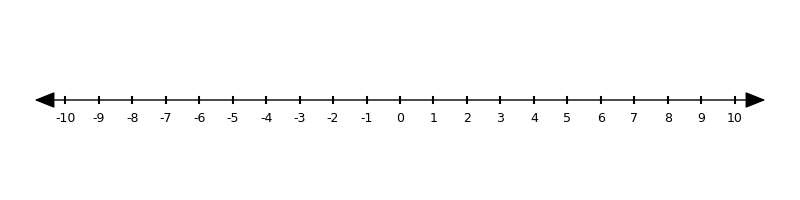
\includegraphics[keepaspectratio]{images/Unit_1/Lesson_1/blank_numberline.png}}

Here, every tick mark is an
\href{./glossary.html\#glossary-integer}{integer} --- a whole number.

\begin{itemize}
\tightlist
\item
  Numbers to the \textbf{right} of zero are
  \href{./glossary.html\#glossary-positive}{positive}
\item
  Numbers to the \textbf{left} of zero are
  \href{./glossary.html\#glossary-negative}{negative}
\end{itemize}

We can use this number line to \emph{see} what happens when we add,
subtract, or compare numbers.

\textbf{Are there other ways to draw a number line?}

Yes! Number lines can be drawn over different ranges and scales. For
example, here is a number line that counts from -10 to 25 in steps of 5.

\pandocbounded{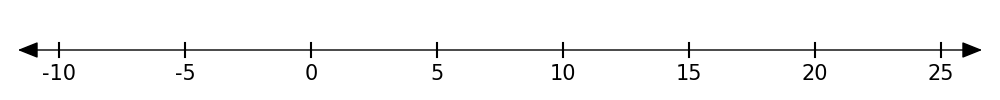
\includegraphics[keepaspectratio]{images/Unit_1/Lesson_1/count_by_5s.png}}

In fact, number lines don't even have to be
\href{./glossary.html\#glossary-horizontal}{horizontal}. Here is a
\href{./glossary.html\#glossary-vertical}{vertical} number line that
goes from 0 to 100 in steps of 10.

\pandocbounded{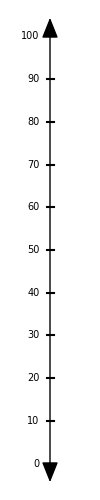
\includegraphics[keepaspectratio]{images/Unit_1/Lesson_1/vertical_by_tens.png}}

\textbf{Example:} How many numbers between 3 and 5?

If you are counting integers, there is 1
\href{./glossary.html\#glossary-integer}{integer} between 3 and 5 (just
4). But if you mean
\href{./glossary.html\#glossary-real-number}{real numbers}, there are
\href{./glossary.html\#glossary-infinitely}{infinitely} many between 3
and 5. Here are some number lines that might help convince you.

\pandocbounded{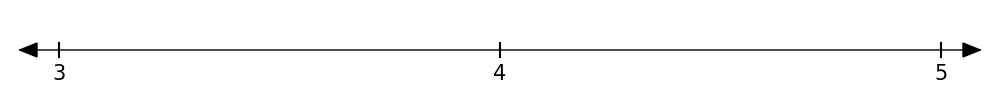
\includegraphics[keepaspectratio]{images/Unit_1/Lesson_1/three_to_five_by_1.png}}
\pandocbounded{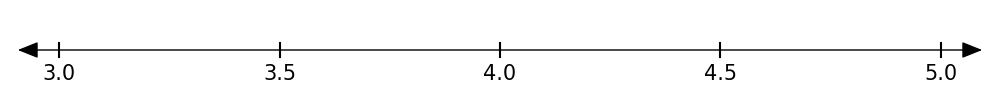
\includegraphics[keepaspectratio]{images/Unit_1/Lesson_1/between_3_and_5_by_05.png}}
\pandocbounded{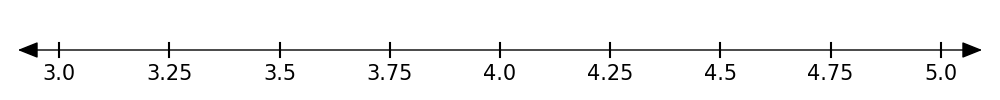
\includegraphics[keepaspectratio]{images/Unit_1/Lesson_1/between_3_and_5_by_025.png}}

Here are a few examples:

\begin{itemize}
\tightlist
\item
  thermometer
\item
  ruler
\item
  timeline
\item
  American football field
\item
  volume slider on a phone
\end{itemize}

\begin{center}\rule{0.5\linewidth}{0.5pt}\end{center}

\subsection*{1.1.2 - Understanding
Opposites}\label{understanding-opposites}
\addcontentsline{toc}{subsection}{1.1.2 - Understanding Opposites}

Let's look at a pair of numbers, 3 and -3.

These are called \href{./glossary.html\#glossary-opposite}{opposite}
numbers. They are the \textbf{same distance} from zero but on
\textbf{opposite sides} of it.

\pandocbounded{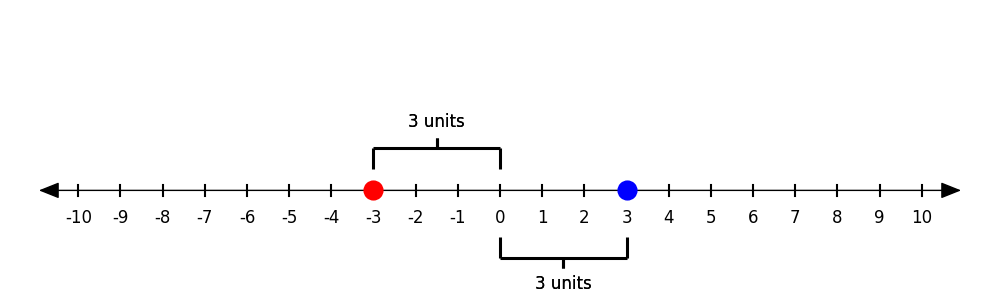
\includegraphics[keepaspectratio]{images/Unit_1/Lesson_1/opposites.png}}

The opposite of zero is zero. Zero is the only number that is its own
opposite!

\begin{center}\rule{0.5\linewidth}{0.5pt}\end{center}

\subsection*{1.1.3 - What Is Absolute
Value?}\label{what-is-absolute-value}
\addcontentsline{toc}{subsection}{1.1.3 - What Is Absolute Value?}

\href{./glossary.html\#glossary-absolute-value}{Absolute value} measures
the \textbf{distance from zero}. Absolute value is written as a number
between two bars. For example, \textbf{the absolute value of -5} is
written \(|-5|\).

Take a look at the number -5. The number line shows that its absolute
value is 5 because it is 5 units away from zero.
\pandocbounded{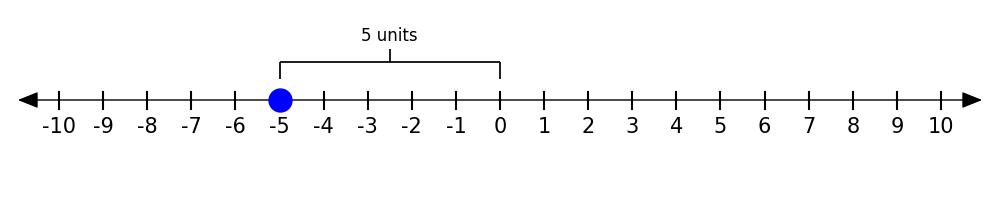
\includegraphics[keepaspectratio]{images/Unit_1/Lesson_1/absolute_value_negative_five.png}}

You can see that \textbar5\textbar{} is also 5 for the same reason!
\pandocbounded{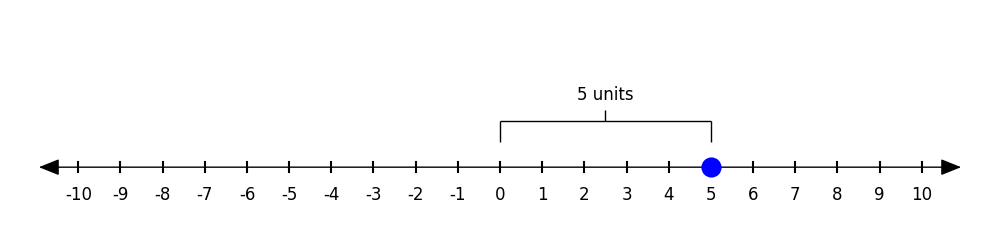
\includegraphics[keepaspectratio]{images/Unit_1/Lesson_1/absolute_value_five.png}}

Absolute value is often used for describing the distance between two
points. Suppose you live 3 miles to the east of the school and your best
friend lives 5 miles to the west. How far apart are your houses? This is
easy to see with a number line.

\pandocbounded{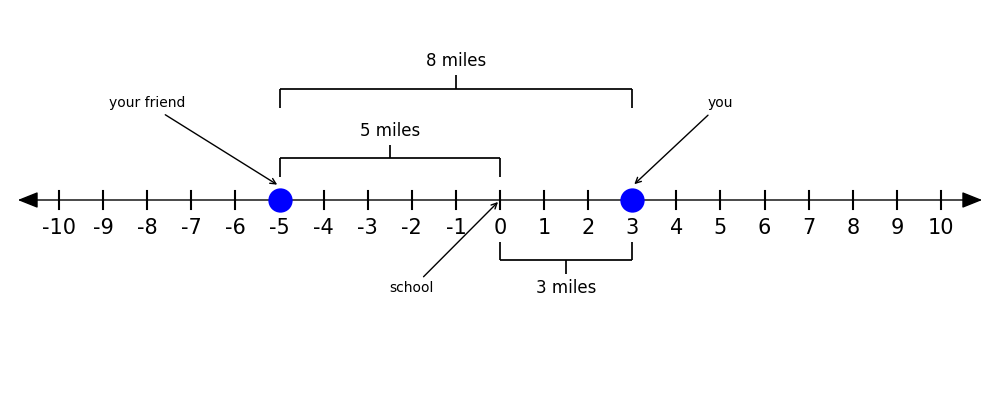
\includegraphics[keepaspectratio]{images/Unit_1/Lesson_1/east_to_west.png}}

You can compute your distances by adding \textbar-5\textbar{} +
\textbar3\textbar, by \textbar-5 - 3\textbar, or by \textbar3 -
(-5)\textbar. All three of these give the same answer, 8 miles. What
would change if we did not use absolute value?

Absolute value is \textbf{never} negative, because distance is never
negative.

\begin{center}\rule{0.5\linewidth}{0.5pt}\end{center}

\subsection*{1.1.4 - Comparing Integers}\label{comparing-integers}
\addcontentsline{toc}{subsection}{1.1.4 - Comparing Integers}

We can also use the number line to compare values.

Let's compare 2 to -7.
\pandocbounded{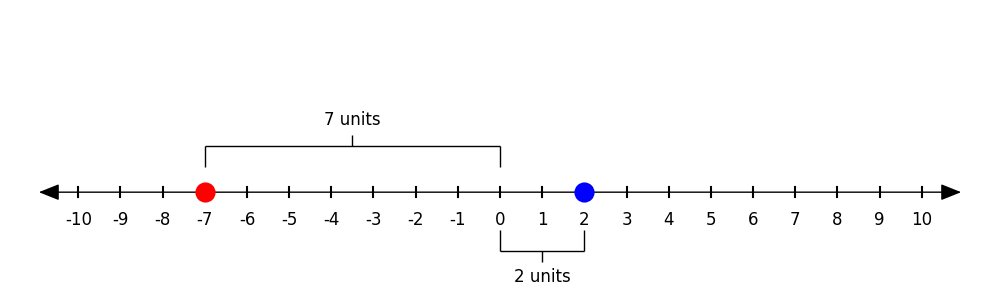
\includegraphics[keepaspectratio]{images/Unit_1/Lesson_1/compare_2_to_neg7.png}}

You can see from the number line that 2 is
\href{./glossary.html\#glossary-greater-than}{greater than}
(\textgreater) -7 because 2 is to the right of -7.

You can also see that -7 is farther from zero than 2 and so
\textbar-7\textbar{} \textgreater{} \textbar2\textbar.

It is easy to get confused here. When we say which number is ``bigger''
(or greater than), we are asking which number is farther to the right on
the number line. This is \textbf{not} the same as absolute value, which
asks which one is furthest from zero.

3 \textgreater{} -8 because it is farther to the right but
\textbar-8\textbar{} \textgreater{} \textbar3\textbar{} because -8 is
farther from zero.

\pandocbounded{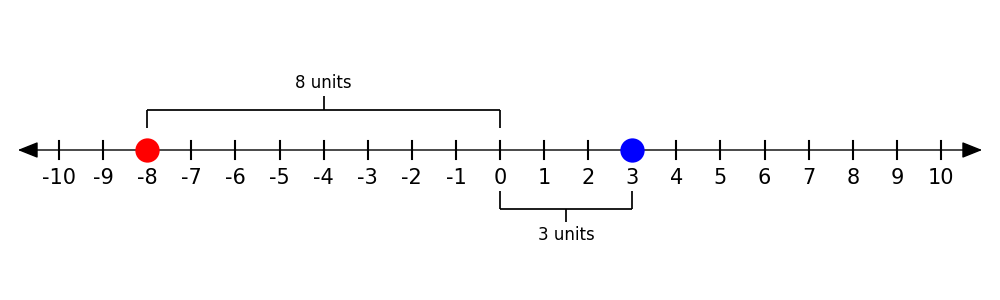
\includegraphics[keepaspectratio]{images/Unit_1/Lesson_1/compare_3_to_neg8.png}}

\begin{center}\rule{0.5\linewidth}{0.5pt}\end{center}

\subsection*{1.1.5 - Number Lines and
Arithmetic}\label{number-lines-and-arithmetic}
\addcontentsline{toc}{subsection}{1.1.5 - Number Lines and Arithmetic}

We can also use the number line to model \textbf{adding and subtracting}
integers.

\begin{itemize}
\tightlist
\item
  To add a \href{./glossary.html\#glossary-positive}{positive} number,
  move \textbf{right}
\item
  To add a \href{./glossary.html\#glossary-negative}{negative} number,
  move \textbf{left}
\end{itemize}

Examples:

\begin{enumerate}
\def\labelenumi{\arabic{enumi}.}
\tightlist
\item
  Addition: \(-2 + 6 = 4\)
  \pandocbounded{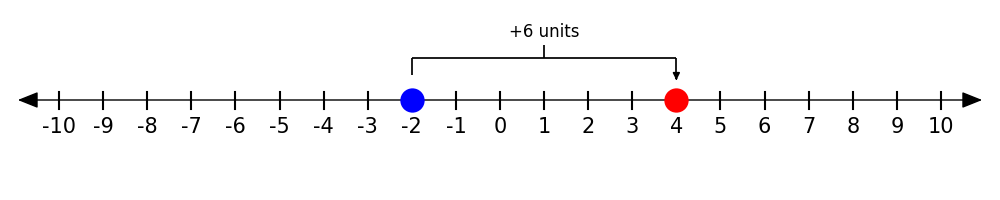
\includegraphics[keepaspectratio]{images/Unit_1/Lesson_1/add_6_to_neg2.png}}
\end{enumerate}

Imagine that you are \$2 in debt. If someone pays you \$6 you can pay
off the debt and have \$\(4\) left over.

\begin{enumerate}
\def\labelenumi{\arabic{enumi}.}
\setcounter{enumi}{1}
\tightlist
\item
  Adding a negative: \(150 + (-5) = 145\)
  \pandocbounded{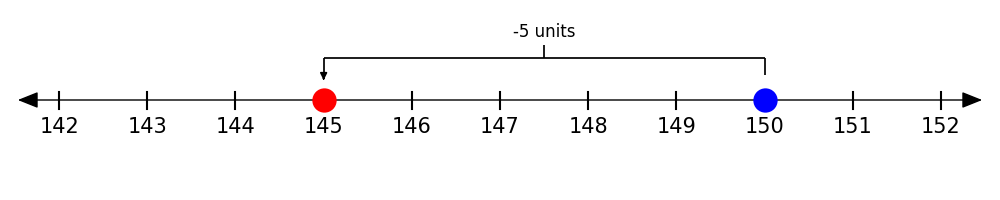
\includegraphics[keepaspectratio]{images/Unit_1/Lesson_1/add_neg5_to_150.png}}
\end{enumerate}

You have \$150 in the bank. The bank adds a fee for being under their
\$200 minimum balance. You now have \$145.

\begin{enumerate}
\def\labelenumi{\arabic{enumi}.}
\setcounter{enumi}{2}
\tightlist
\item
  Subtraction: \(400 - 450 = -50\)
  \pandocbounded{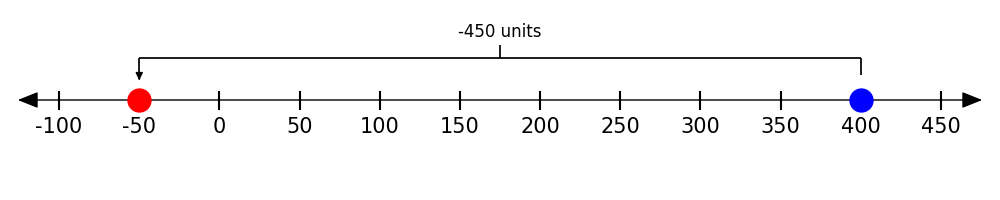
\includegraphics[keepaspectratio]{images/Unit_1/Lesson_1/subtract_450_from_400.png}}
\end{enumerate}

If you only have \$400 but spend \$450 on a credit card, you are now
\$50 in debt.

\begin{enumerate}
\def\labelenumi{\arabic{enumi}.}
\setcounter{enumi}{3}
\tightlist
\item
  Subtracting a negative: \(201 - (-5) = 206\)
  \pandocbounded{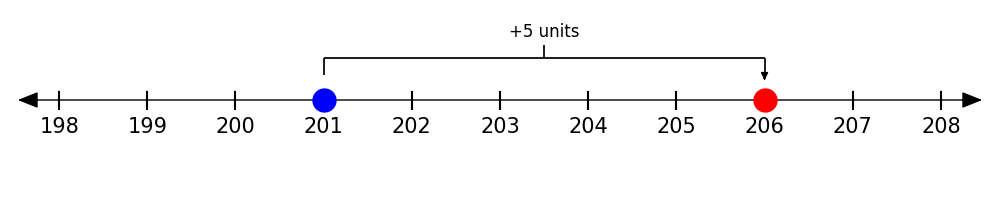
\includegraphics[keepaspectratio]{images/Unit_1/Lesson_1/subtract_neg5_from_201.png}}
\end{enumerate}

\begin{quote}
Example: The bank made a mistake, you had \$\(201\) in your account so
they took off the \$\(5\) fee. Now you have \$\(206\).
\end{quote}

\begin{center}\rule{0.5\linewidth}{0.5pt}\end{center}

\section*{✍️ Practice On Your Own}\label{practice-on-your-own}
\addcontentsline{toc}{section}{✍️ Practice On Your Own}

\markright{✍️ Practice On Your Own}

\textbf{Working With Number Lines}

\begin{enumerate}
\def\labelenumi{\arabic{enumi}.}
\item
  Draw a number line that shows:

  \begin{enumerate}
  \def\labelenumii{\alph{enumii}.}
  \item
    -4, 0, and 3.
  \item
    Your age
  \item
    The number halfway between 5 and 9.
  \end{enumerate}
\item
  What question could match this number line?

  \pandocbounded{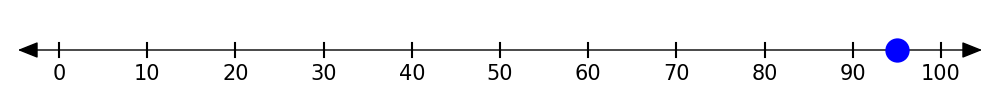
\includegraphics[keepaspectratio]{images/Unit_1/Lesson_1/problem_2.png}}
\end{enumerate}

\begin{center}\rule{0.5\linewidth}{0.5pt}\end{center}

\textbf{Opposites}

\begin{enumerate}
\def\labelenumi{\arabic{enumi}.}
\setcounter{enumi}{2}
\item
  What is the opposite of 42?
\item
  What is the opposite of -3?
\item
  Draw a number line with two numbers that are opposites.
\item
  Does 3.5 have an opposite? If yes, what is it?
\end{enumerate}

\begin{center}\rule{0.5\linewidth}{0.5pt}\end{center}

\textbf{Comparing Numbers}

\begin{enumerate}
\def\labelenumi{\arabic{enumi}.}
\setcounter{enumi}{6}
\item
  Which number is \textbf{greater}, 5 or -10?
\item
  Which number has the greater absolute value, 5 or -10?
\item
  Is 28 bigger than -30?
\item
  Use (\textbf{\textgreater{}}) or (\textbf{\textless{}}) to compare:

  \begin{enumerate}
  \def\labelenumii{\alph{enumii}.}
  \item
    -11~\_\_\_~-13
  \item
    7~\_\_\_~-2
  \item
    \textbar-3\textbar~\_\_\_~\textbar5\textbar{}
  \end{enumerate}
\item
  Which is bigger?

  \begin{enumerate}
  \def\labelenumii{\alph{enumii}.}
  \item
    -4 or -5
  \item
    3 or the opposite of 7
  \item
    \textbar-5\textbar{} or \textbar4\textbar{}
  \end{enumerate}
\item
  Use a number line to compare:

  \begin{enumerate}
  \def\labelenumii{\alph{enumii}.}
  \item
    -7 to 2.
  \item
    The year you were born and the current year
  \end{enumerate}
\end{enumerate}

\begin{center}\rule{0.5\linewidth}{0.5pt}\end{center}

\textbf{Addition and Subtraction}

\begin{enumerate}
\def\labelenumi{\arabic{enumi}.}
\setcounter{enumi}{12}
\item
  Show these on a number line:

  \begin{enumerate}
  \def\labelenumii{\alph{enumii}.}
  \item
    \(-3 + 5\)
  \item
    \(3 - 5\)
  \item
    \(-3 + (-3)\)
  \item
    \(3 - (-3)\)
  \end{enumerate}
\end{enumerate}

\begin{center}\rule{0.5\linewidth}{0.5pt}\end{center}

\textbf{Word Problems}

\begin{enumerate}
\def\labelenumi{\arabic{enumi}.}
\setcounter{enumi}{13}
\item
  Solve using a number line

  \begin{enumerate}
  \def\labelenumii{\alph{enumii}.}
  \item
    The temperature was -12°F. It warms up by 20°. What is the new
    temperature?
  \item
    A diver is 45 feet below sea level. She dives 30 feet deeper. How
    far down is she?
  \item
    Your bank account is at -\$8. You deposit \$5. What is your new
    balance?
  \end{enumerate}
\end{enumerate}

\begin{center}\rule{0.5\linewidth}{0.5pt}\end{center}

\textbf{Warm-Up}

\begin{enumerate}
\def\labelenumi{\arabic{enumi}.}
\item
  6
\item
  -4
\item
  -7
\end{enumerate}

\begin{center}\rule{0.5\linewidth}{0.5pt}\end{center}

\textbf{Working With Number Lines}

\begin{enumerate}
\def\labelenumi{\arabic{enumi}.}
\item
  \begin{enumerate}
  \def\labelenumii{\alph{enumii}.}
  \item
    \pandocbounded{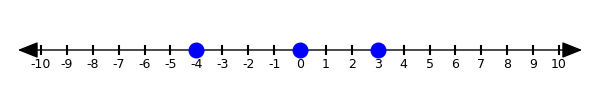
\includegraphics[keepaspectratio]{images/Unit_1/Lesson_1/answer_1_a.png}}
  \item
    \emph{Answers vary. Here is what a 15-year-old would show:}

    \pandocbounded{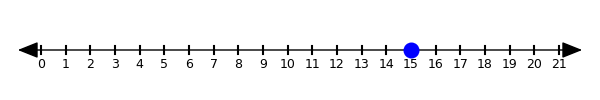
\includegraphics[keepaspectratio]{images/Unit_1/Lesson_1/answer_1_b.png}}
  \item
    7

    \pandocbounded{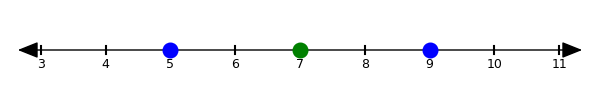
\includegraphics[keepaspectratio]{images/Unit_1/Lesson_1/answer_1_c.png}}
  \end{enumerate}
\item
  \emph{Example question:} ``What was the temperature on July 4th?''

  \pandocbounded{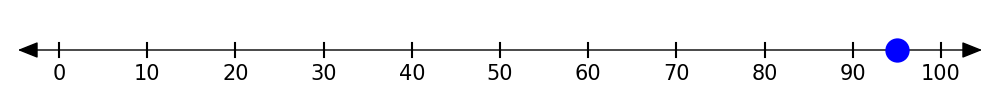
\includegraphics[keepaspectratio]{images/Unit_1/Lesson_1/problem_2.png}}
\end{enumerate}

\begin{center}\rule{0.5\linewidth}{0.5pt}\end{center}

\textbf{Opposites}

\begin{enumerate}
\def\labelenumi{\arabic{enumi}.}
\setcounter{enumi}{2}
\item
  -42
\item
  3
\item
  \emph{Answers vary. Example:}

  \pandocbounded{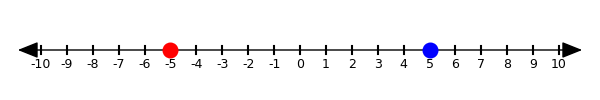
\includegraphics[keepaspectratio]{images/Unit_1/Lesson_1/answer_5.png}}
\item
  Yes --- the opposite is -3.5
\end{enumerate}

\begin{center}\rule{0.5\linewidth}{0.5pt}\end{center}

\textbf{Comparing Numbers}

\begin{enumerate}
\def\labelenumi{\arabic{enumi}.}
\setcounter{enumi}{6}
\item
  5 is greater (farther right on the number line)
\item
  -10 has the greater absolute value (10 \textgreater{} 5)
\item
  Yes --- 28 is greater because it is to the right of -30
\item
  \begin{enumerate}
  \def\labelenumii{\alph{enumii}.}
  \tightlist
  \item
    -11 \textgreater{} -13
  \item
    7 \textgreater{} -2
  \item
    \textbar-3\textbar{} \textless{} \textbar5\textbar{} (3 \textless{}
    5)
  \end{enumerate}
\item
  \begin{enumerate}
  \def\labelenumii{\alph{enumii}.}
  \tightlist
  \item
    -4 \textgreater{} -5
  \item
    3 \textgreater{} -7
  \item
    \textbar-5\textbar{} \textgreater{} \textbar4\textbar{} (5
    \textgreater{} 4)
  \end{enumerate}
\item
  \begin{enumerate}
  \def\labelenumii{\alph{enumii}.}
  \item
    2 \textgreater{} -7
  \item
    \emph{Answers vary --- for example, 2025 \textgreater{} 1985}

    \pandocbounded{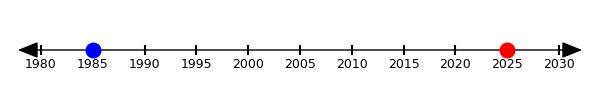
\includegraphics[keepaspectratio]{images/Unit_1/Lesson_1/answer_12_b.png}}
  \end{enumerate}
\end{enumerate}

\begin{center}\rule{0.5\linewidth}{0.5pt}\end{center}

\textbf{Addition and Subtraction}

\begin{enumerate}
\def\labelenumi{\arabic{enumi}.}
\setcounter{enumi}{12}
\tightlist
\item
  \begin{enumerate}
  \def\labelenumii{\alph{enumii}.}
  \tightlist
  \item
    \pandocbounded{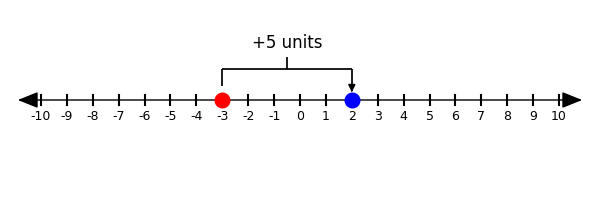
\includegraphics[keepaspectratio]{images/Unit_1/Lesson_1/answer_13_a.png}}
  \item
    \pandocbounded{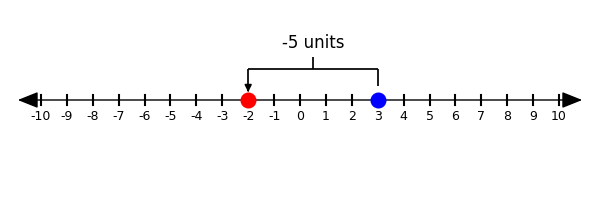
\includegraphics[keepaspectratio]{images/Unit_1/Lesson_1/answer_13_b.png}}
  \item
    \pandocbounded{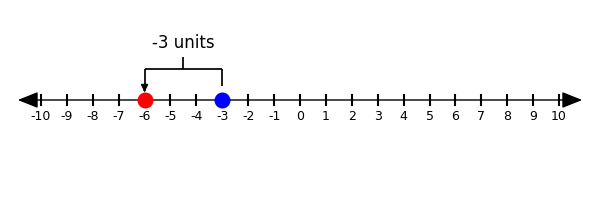
\includegraphics[keepaspectratio]{images/Unit_1/Lesson_1/answer_13_c.png}}
  \item
    \pandocbounded{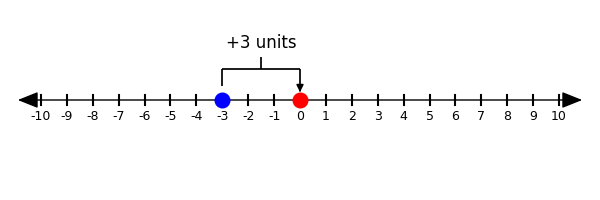
\includegraphics[keepaspectratio]{images/Unit_1/Lesson_1/answer_13_d.png}}
  \end{enumerate}
\end{enumerate}

\begin{center}\rule{0.5\linewidth}{0.5pt}\end{center}

\textbf{Word Problems}

\begin{enumerate}
\def\labelenumi{\arabic{enumi}.}
\setcounter{enumi}{13}
\item
  \begin{enumerate}
  \def\labelenumii{\alph{enumii}.}
  \item
    8°F

    \pandocbounded{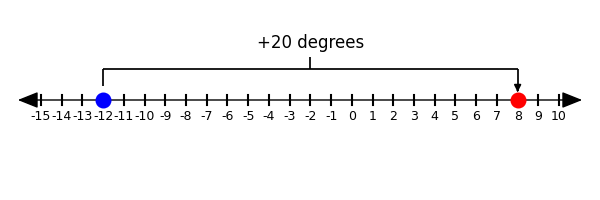
\includegraphics[keepaspectratio]{images/Unit_1/Lesson_1/answer_14_a.png}}
  \item
    75 feet down

    \pandocbounded{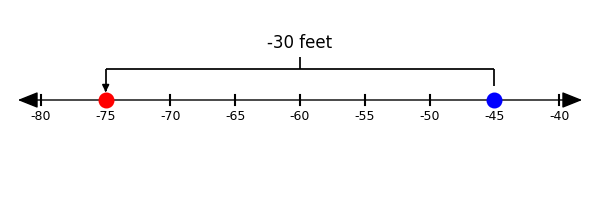
\includegraphics[keepaspectratio]{images/Unit_1/Lesson_1/answer_14_b.png}}
  \item
    -\$3

    \pandocbounded{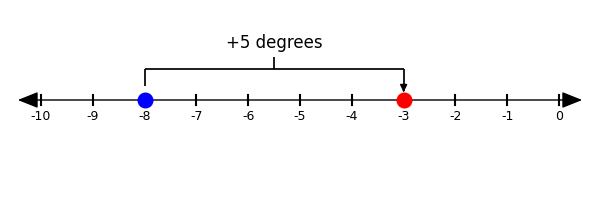
\includegraphics[keepaspectratio]{images/Unit_1/Lesson_1/answer_14_c.png}}
  \end{enumerate}
\end{enumerate}

\chapter*{1.2 - Factors, Multiples \& Prime
Factorization}\label{factors-multiples-prime-factorization}
\addcontentsline{toc}{chapter}{1.2 - Factors, Multiples \& Prime
Factorization}

\markboth{1.2 - Factors, Multiples \& Prime Factorization}{1.2 -
Factors, Multiples \& Prime Factorization}

Have you ever had to split something up evenly --- like slices of pizza
or players on a team? That's really what
\href{./glossary.html\#glossary-factor}{factors} are about: dividing
numbers into equal parts.

In this lesson, you'll learn how to:

\begin{itemize}
\item
  Spot factors and \href{./glossary.html\#glossary-multiple}{multiples}.
\item
  Tell if a number is
  \href{./glossary.html\#glossary-prime-number}{prime number} or
  \href{./glossary.html\#glossary-composite-number}{composite number}.
\item
  Break numbers into their basic building blocks using a
  \href{./glossary.html\#glossary-factor-tree}{factor tree}.
\end{itemize}

You'll use these skills again and again --- from simplifying fractions
to solving equations.

\begin{itemize}
\tightlist
\item[$\square$]
  I can find the factors and multiples of integers
\item[$\square$]
  I can tell if a number is prime or composite
\item[$\square$]
  I can break numbers into prime factors using a factor tree
\end{itemize}

\href{./glossary.html\#glossary-composite-number}{composite number},
\href{./glossary.html\#glossary-factor}{factor},
\href{./glossary.html\#glossary-factor-tree}{factor tree},
\href{./glossary.html\#glossary-multiple}{multiple},
\href{./glossary.html\#glossary-prime-factorization}{prime factorization},
\href{./glossary.html\#glossary-prime-number}{prime number}

\section*{🔥 Warm-Up}\label{warm-up-1}
\addcontentsline{toc}{section}{🔥 Warm-Up}

\markright{🔥 Warm-Up}

\begin{enumerate}
\def\labelenumi{\arabic{enumi}.}
\item
  How many different pairs of whole numbers can you multiply to get 36?
\item
  How many whole numbers can you multiply by 7 and still get a result
  less than 50?
\item
  Can you find more than one pair of whole numbers that multiply to make
  13?
\end{enumerate}

\begin{center}\rule{0.5\linewidth}{0.5pt}\end{center}

\section*{👥 Learn Together}\label{learn-together-1}
\addcontentsline{toc}{section}{👥 Learn Together}

\markright{👥 Learn Together}

\subsection*{1.2.1 - What Are Factors?}\label{what-are-factors}
\addcontentsline{toc}{subsection}{1.2.1 - What Are Factors?}

A \href{./glossary.html\#glossary-factor}{factor} of a number is a whole
number that divides it evenly --- with no
\href{./glossary.html\#glossary-remainder}{remainder}.

\textbf{Example:}

The factors of 12 are: 1, 2, 3, 4, 6 and 12

That's because:

1 × 12 = 12

2 × 6 = 12

3 × 4 = 12

Only one number does: \textbf{1}. It only has itself as a factor!

\begin{center}\rule{0.5\linewidth}{0.5pt}\end{center}

\subsection*{1.2.2 - What Are Multiples?}\label{what-are-multiples}
\addcontentsline{toc}{subsection}{1.2.2 - What Are Multiples?}

A \href{./glossary.html\#glossary-multiple}{multiple} is what you get
when you multiply a number by 1, 2, 3, 4\ldots{}

\textbf{Example:}

Here are the first few multiples of 5:

\(5, 10, 15, 20, 25, 30, ...\)

\textbf{Where have we seen this before?}

Multiples show up all over the place. When you
\href{./glossary.html\#glossary-skip-count}{skip count}, you are using
multiples. In the previous lesson, we used multiples to construct number
lines!

\textbf{Example:}

Here is a number line that shows multiples of three.
\pandocbounded{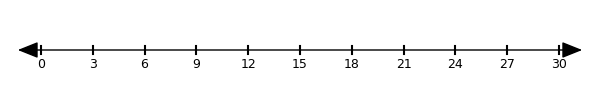
\includegraphics[keepaspectratio]{images/Unit_1/Lesson_2/skip_count_by_3.png}}

If a bus comes every 15 minutes, the arrival times are multiples of 15.

\begin{center}\rule{0.5\linewidth}{0.5pt}\end{center}

\subsection*{1.2.3 - Prime vs.~Composite}\label{prime-vs.-composite}
\addcontentsline{toc}{subsection}{1.2.3 - Prime vs.~Composite}

Some numbers can only be divided evenly two ways --- others can be
broken into many parts. Let's explore the difference between
\href{./glossary.html\#glossary-prime-number}{prime numbers} and
\href{./glossary.html\#glossary-composite-number}{composite numbers}.

A \textbf{prime number} has only 2 factors: 1 and itself.

Examples: 2, 3, 5, 7, 11, 13\ldots{}

A \textbf{composite number} has more than 2 factors.

Examples: 4, 6, 8, 9, 10\ldots{}

People around the world spend years searching for giant prime numbers.
The largest ones we've found so far have over 24 million digits!

Why go to all that trouble?

Prime numbers are the secret behind modern encryption. They're used to
protect everything from bank accounts to private messages. The bigger
the primes, the harder they are to break --- which is why finding huge
ones is such a big deal.

It's like a global math scavenger hunt\ldots{} with real-world
consequences.

\begin{center}\rule{0.5\linewidth}{0.5pt}\end{center}

\subsection*{1.2.4 - Prime Factorization and Factor
Trees}\label{prime-factorization-and-factor-trees}
\addcontentsline{toc}{subsection}{1.2.4 - Prime Factorization and Factor
Trees}

Every number can be broken into a
\href{./glossary.html\#glossary-product}{product} of prime numbers ---
sort of like breaking a LEGO® sculpture into individual bricks. These
prime factors are the basic building blocks of all whole numbers.

We use \textbf{factor trees} to find these prime factors. This isn't
just a fun trick --- it builds your
\href{./glossary.html\#glossary-number-sense}{number sense}: your
ability to see patterns, understand how numbers are structured, and work
confidently with them.

That number sense will come in handy later when you:

\begin{itemize}
\tightlist
\item
  Simplify fractions
\item
  Solve equations
\item
  Factor algebraic expressions
\end{itemize}

Let's build a factor tree for \textbf{360} to see how it works.

\begin{center}\rule{0.5\linewidth}{0.5pt}\end{center}

\subsubsection*{Steps to Make a Factor
Tree}\label{steps-to-make-a-factor-tree}
\addcontentsline{toc}{subsubsection}{Steps to Make a Factor Tree}

\begin{enumerate}
\def\labelenumi{\arabic{enumi}.}
\tightlist
\item
  Start with a number:
\end{enumerate}

\phantomsection\label{mermaid-diagram}
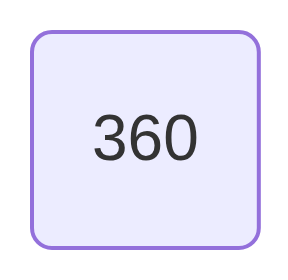
\includegraphics[width=0.76in,height=0.73in]{chapters/Unit_1/1.2_Factors_Multiples_&_Prime_Factorization_files/figure-latex/mermaid-figure-1.png}

2. Find any two numbers that multiply to give the number:
\(360 = 18 × 20\)

\phantomsection\label{mermaid-diagram}
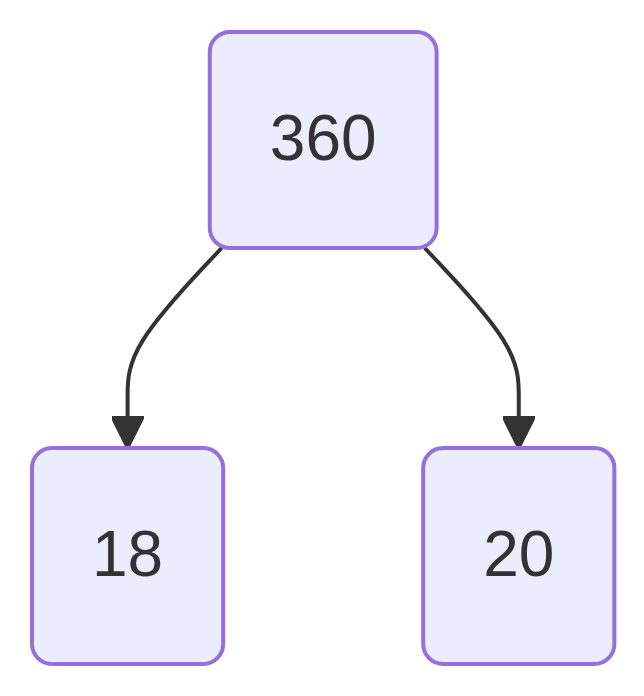
\includegraphics[width=1.68in,height=1.81in]{chapters/Unit_1/1.2_Factors_Multiples_&_Prime_Factorization_files/figure-latex/mermaid-figure-9.png}

3. Break each of those numbers down further:

\begin{itemize}
\tightlist
\item
  \(18 = 3 × 6\)
\item
  \(20 = 4 × 5\)
\end{itemize}

\phantomsection\label{mermaid-diagram}
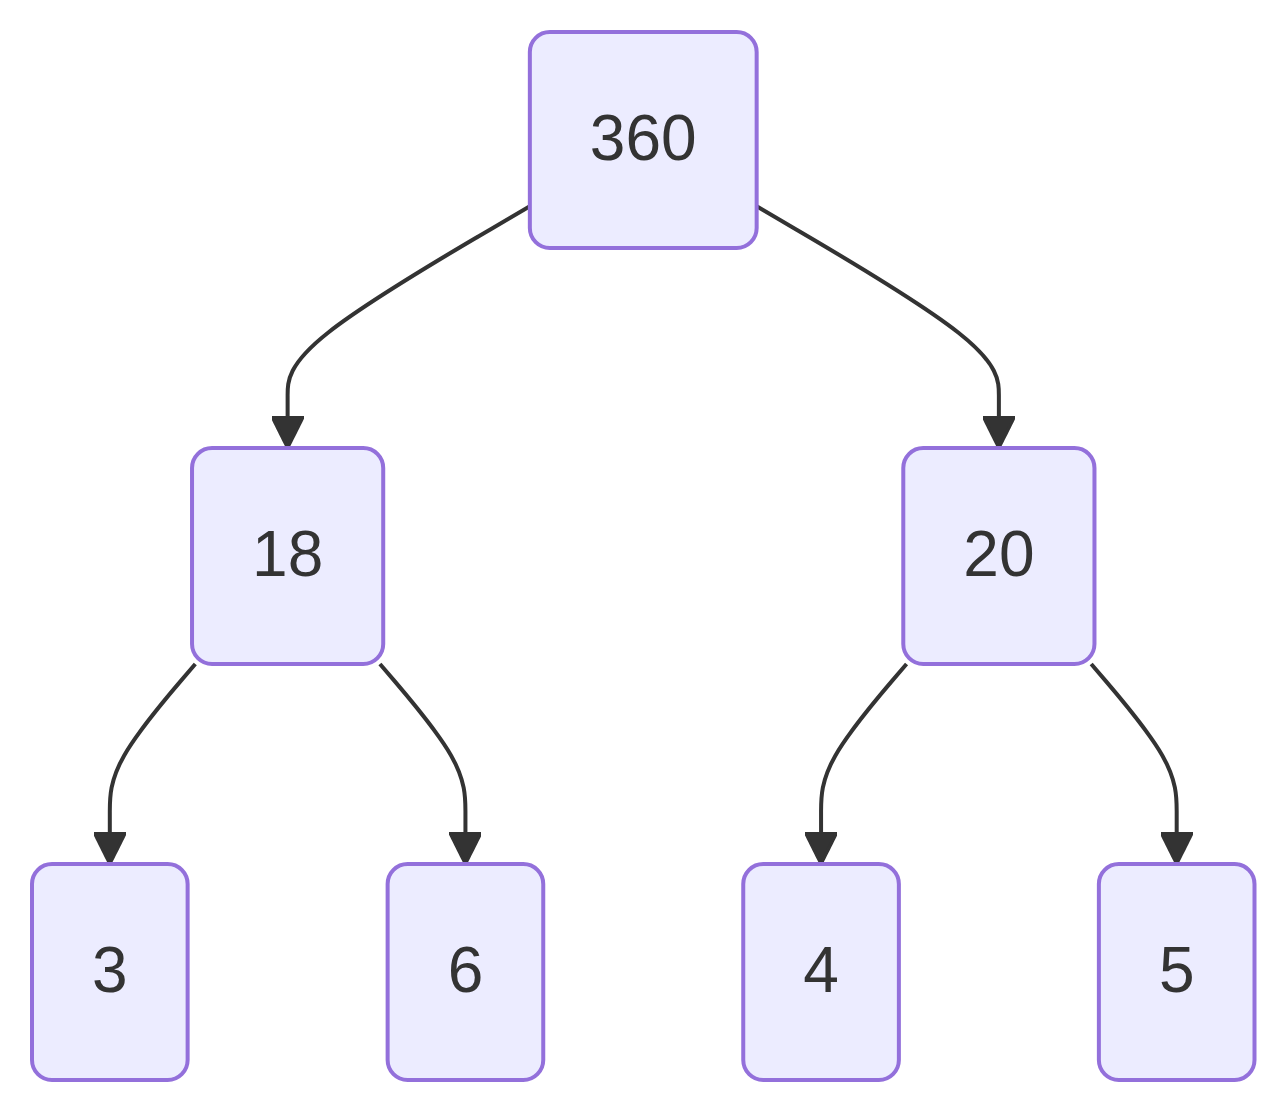
\includegraphics[width=3.35in,height=2.9in]{chapters/Unit_1/1.2_Factors_Multiples_&_Prime_Factorization_files/figure-latex/mermaid-figure-8.png}

4. Keep going until all branches end in \textbf{prime numbers} (numbers
that can't be factored anymore, like 2, 3, 5, 7\ldots). We call the ends
of the branches ``leaves''.

\phantomsection\label{mermaid-diagram}
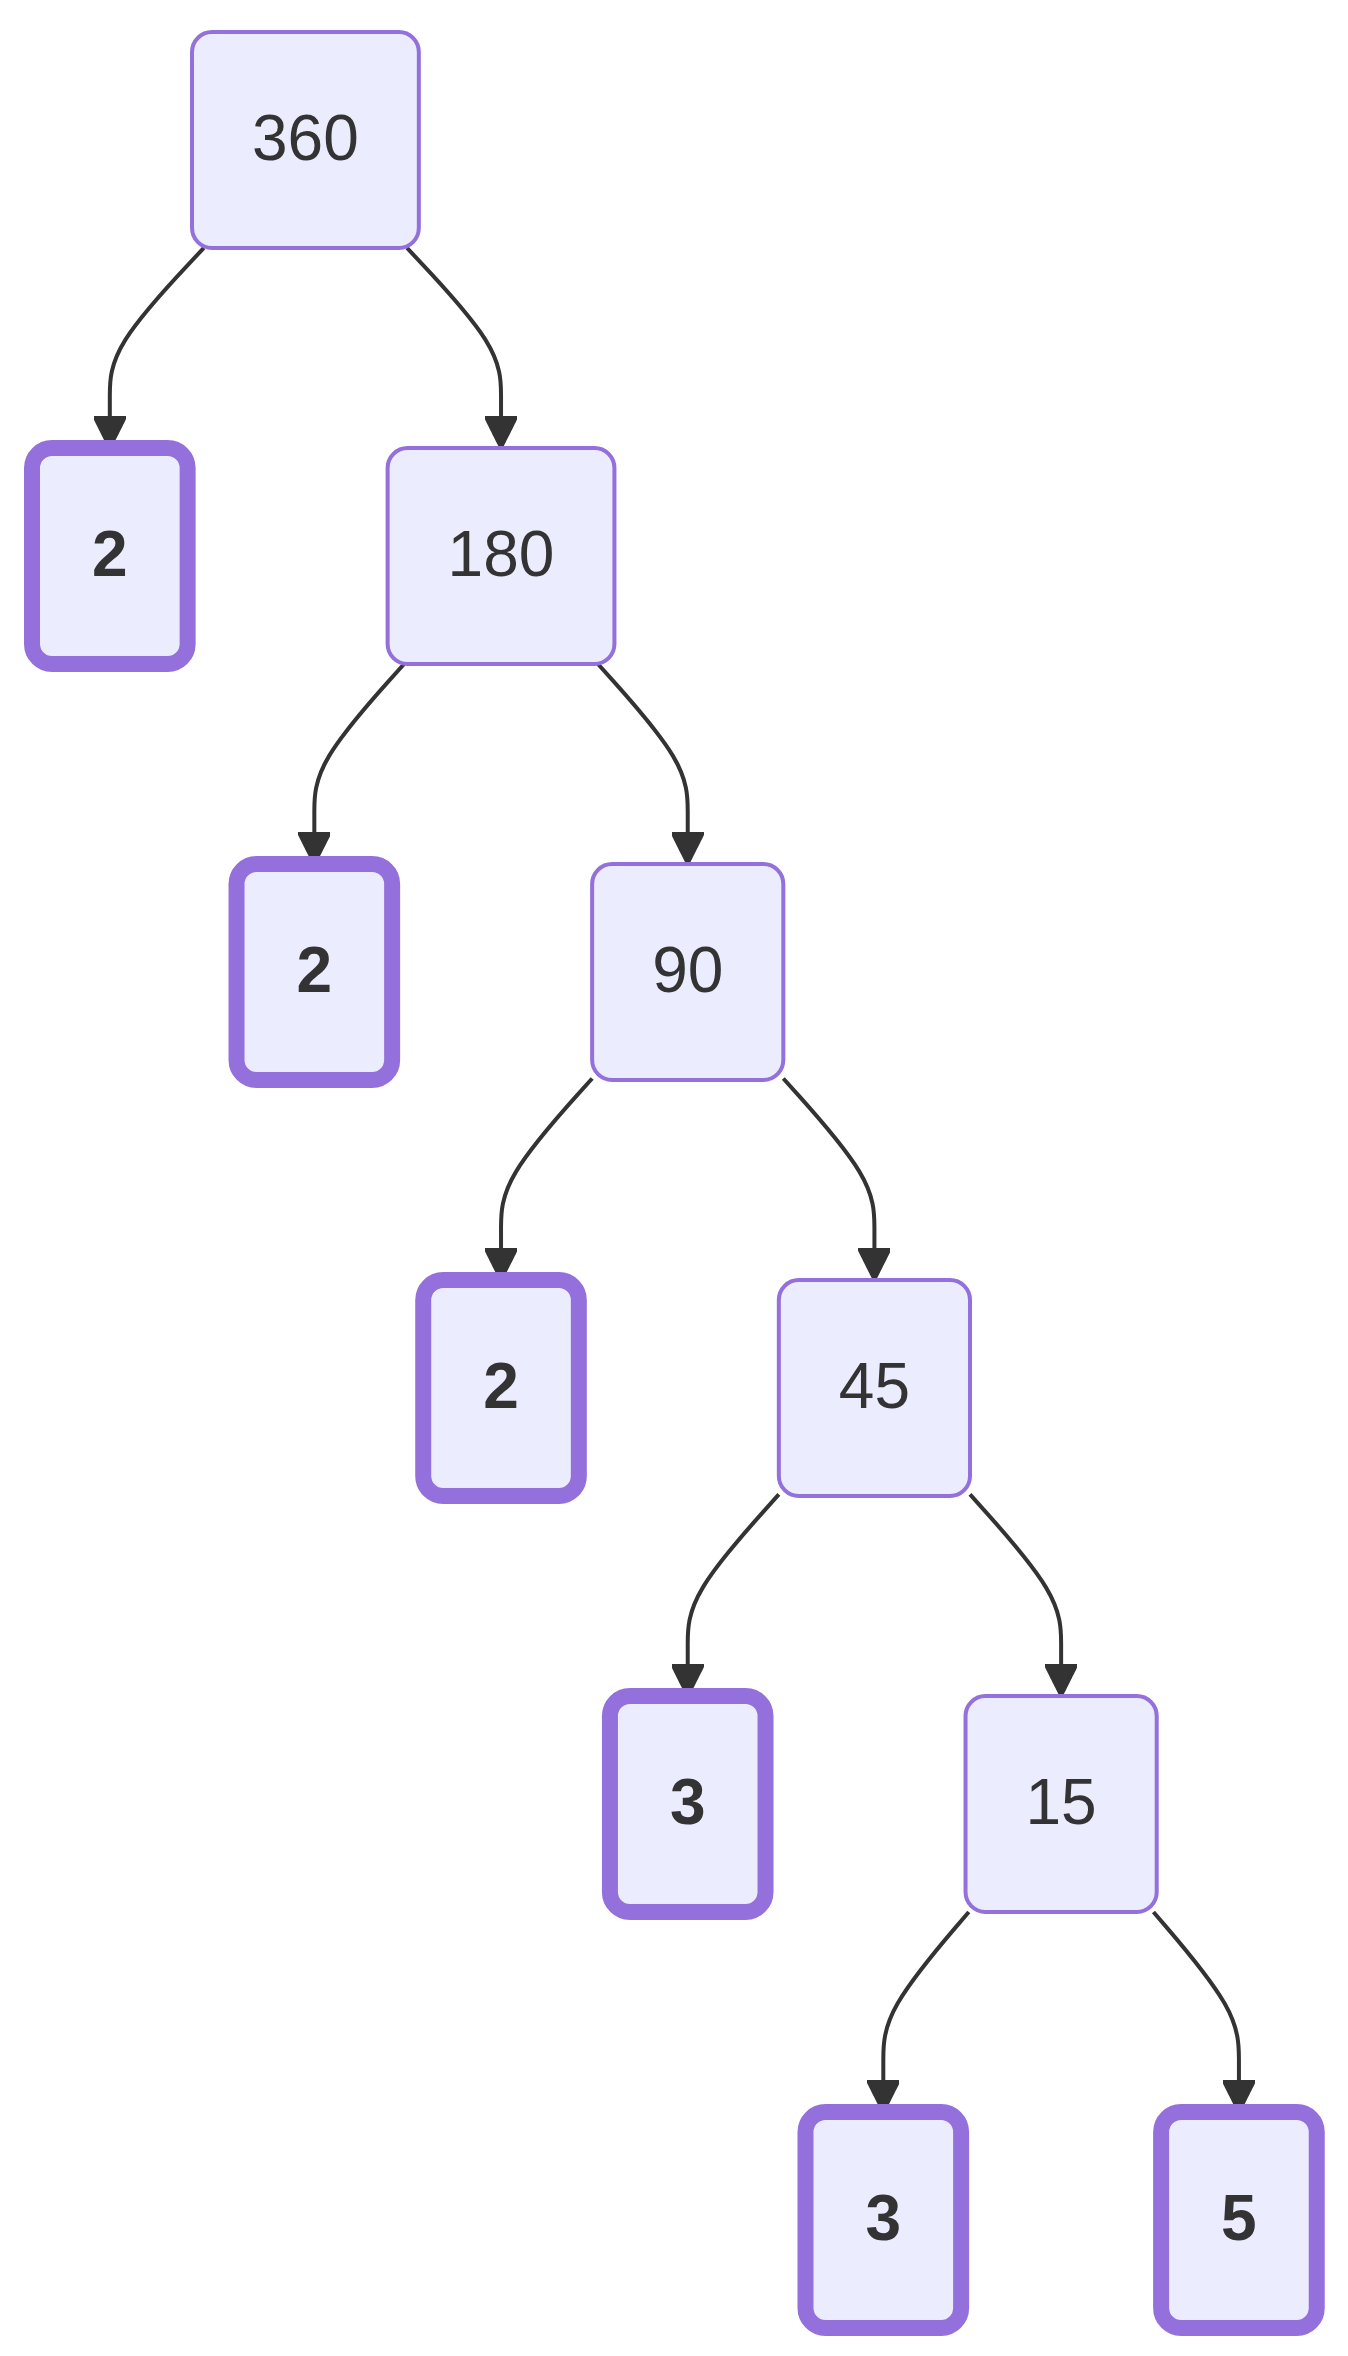
\includegraphics[width=4.28in,height=3.98in]{chapters/Unit_1/1.2_Factors_Multiples_&_Prime_Factorization_files/figure-latex/mermaid-figure-7.png}

5. The prime factorization is the product of the leaves of the tree:
\[2 * 2 * 2 * 3 * 3 * 5 = 360\] This can be written more compactly by
using the factor counts as
\href{./glossary.html\#glossary-exponent}{exponents}. There are three 2s
and two 3s in this case and so we get\ldots{} \[2^3 * 3^2 * 5 = 360\]

\begin{center}\rule{0.5\linewidth}{0.5pt}\end{center}

There are \emph{many} factor trees for the number 360. For example, you
could also have started with \(360 = 3 * 120\).

\phantomsection\label{mermaid-diagram}
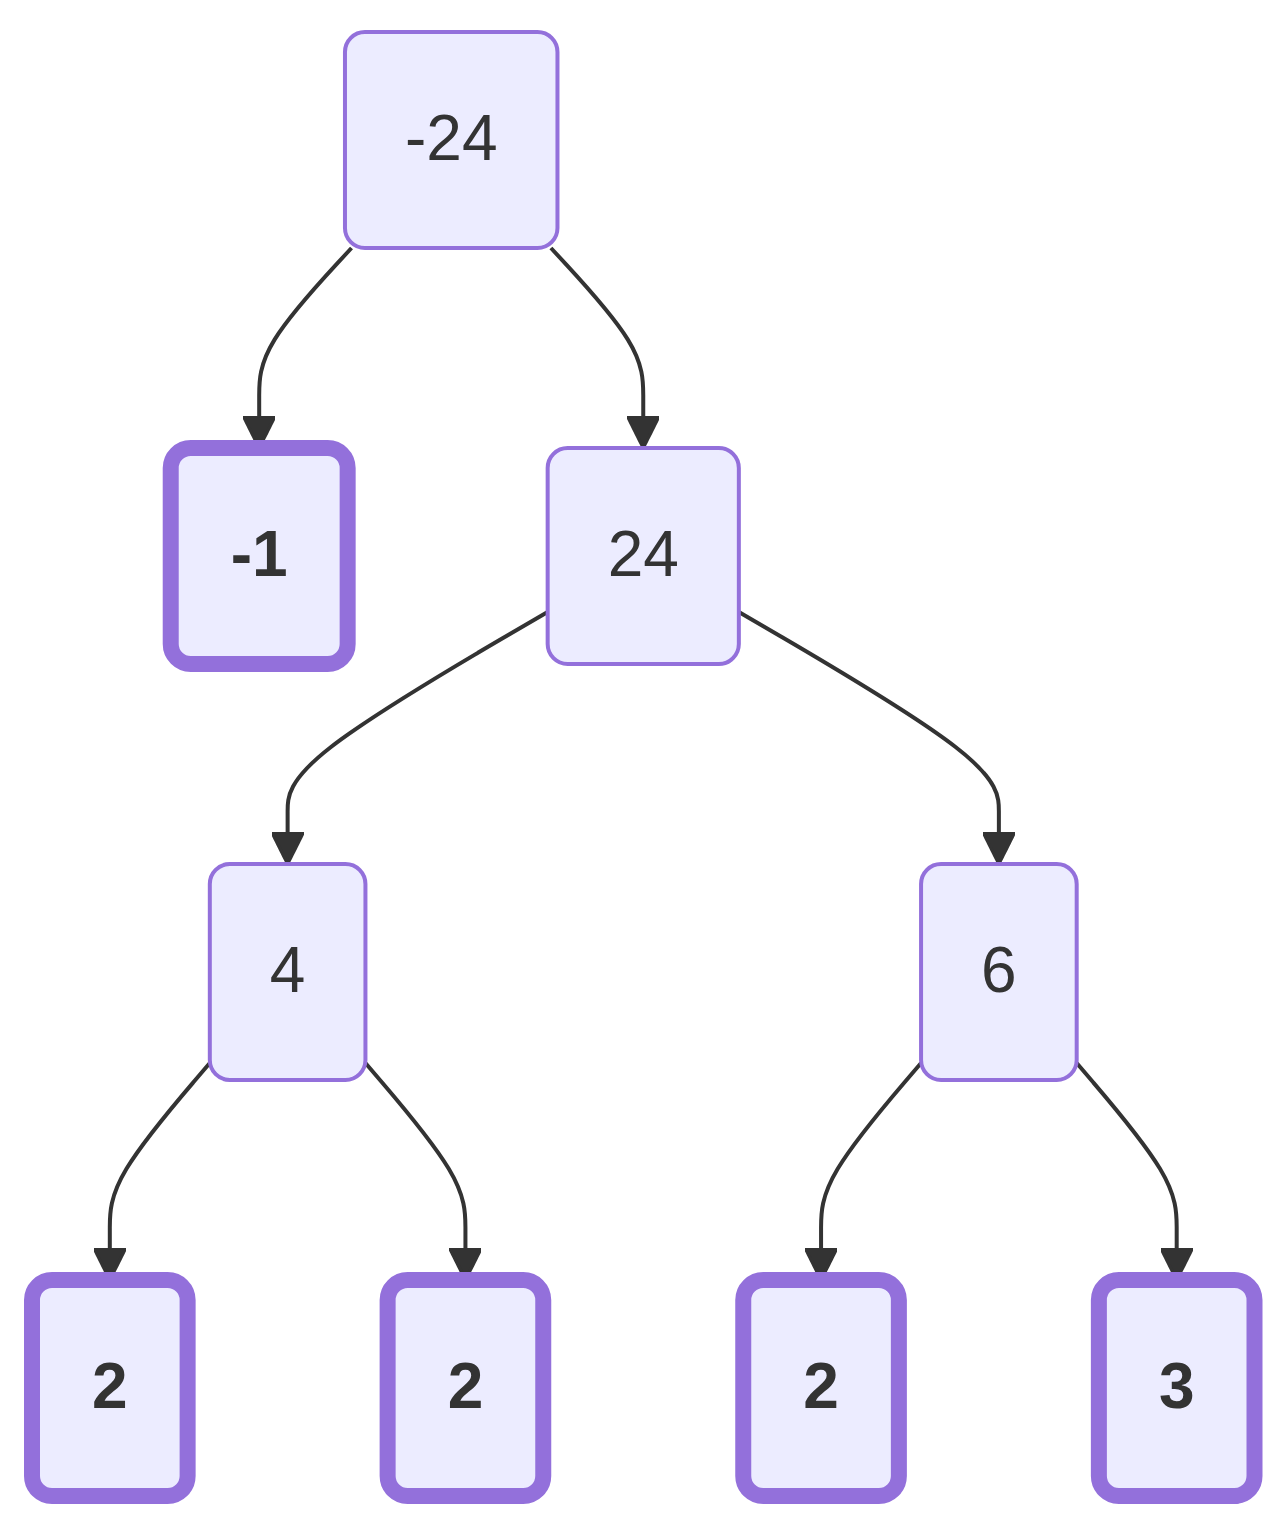
\includegraphics[width=3.47in,height=5.06in]{chapters/Unit_1/1.2_Factors_Multiples_&_Prime_Factorization_files/figure-latex/mermaid-figure-6.png}

There are still three 2s, two 3s, and one 5, so the prime factorization
does not change! \[2^3 * 3^2 * 5 = 360\] As long as you end up with the
same prime numbers, the tree is correct!

\begin{center}\rule{0.5\linewidth}{0.5pt}\end{center}

\begin{tcolorbox}[enhanced jigsaw, left=2mm, opacityback=0, colback=white, rightrule=.15mm, toptitle=1mm, colframe=quarto-callout-tip-color-frame, leftrule=.75mm, toprule=.15mm, breakable, bottomtitle=1mm, bottomrule=.15mm, colbacktitle=quarto-callout-tip-color!10!white, arc=.35mm, opacitybacktitle=0.6, titlerule=0mm, coltitle=black, title=\textcolor{quarto-callout-tip-color}{\faLightbulb}\hspace{0.5em}{Which factors should I start with?}]

There is no one right answer to this question. It depends on your goal.
If your goal is finding easy numbers, you might start small. Notice that
360 is \href{./glossary.html\#glossary-even}{even}, that means it is
divisible by 2. We could divide by 2 and keep going that way.

\phantomsection\label{mermaid-diagram}
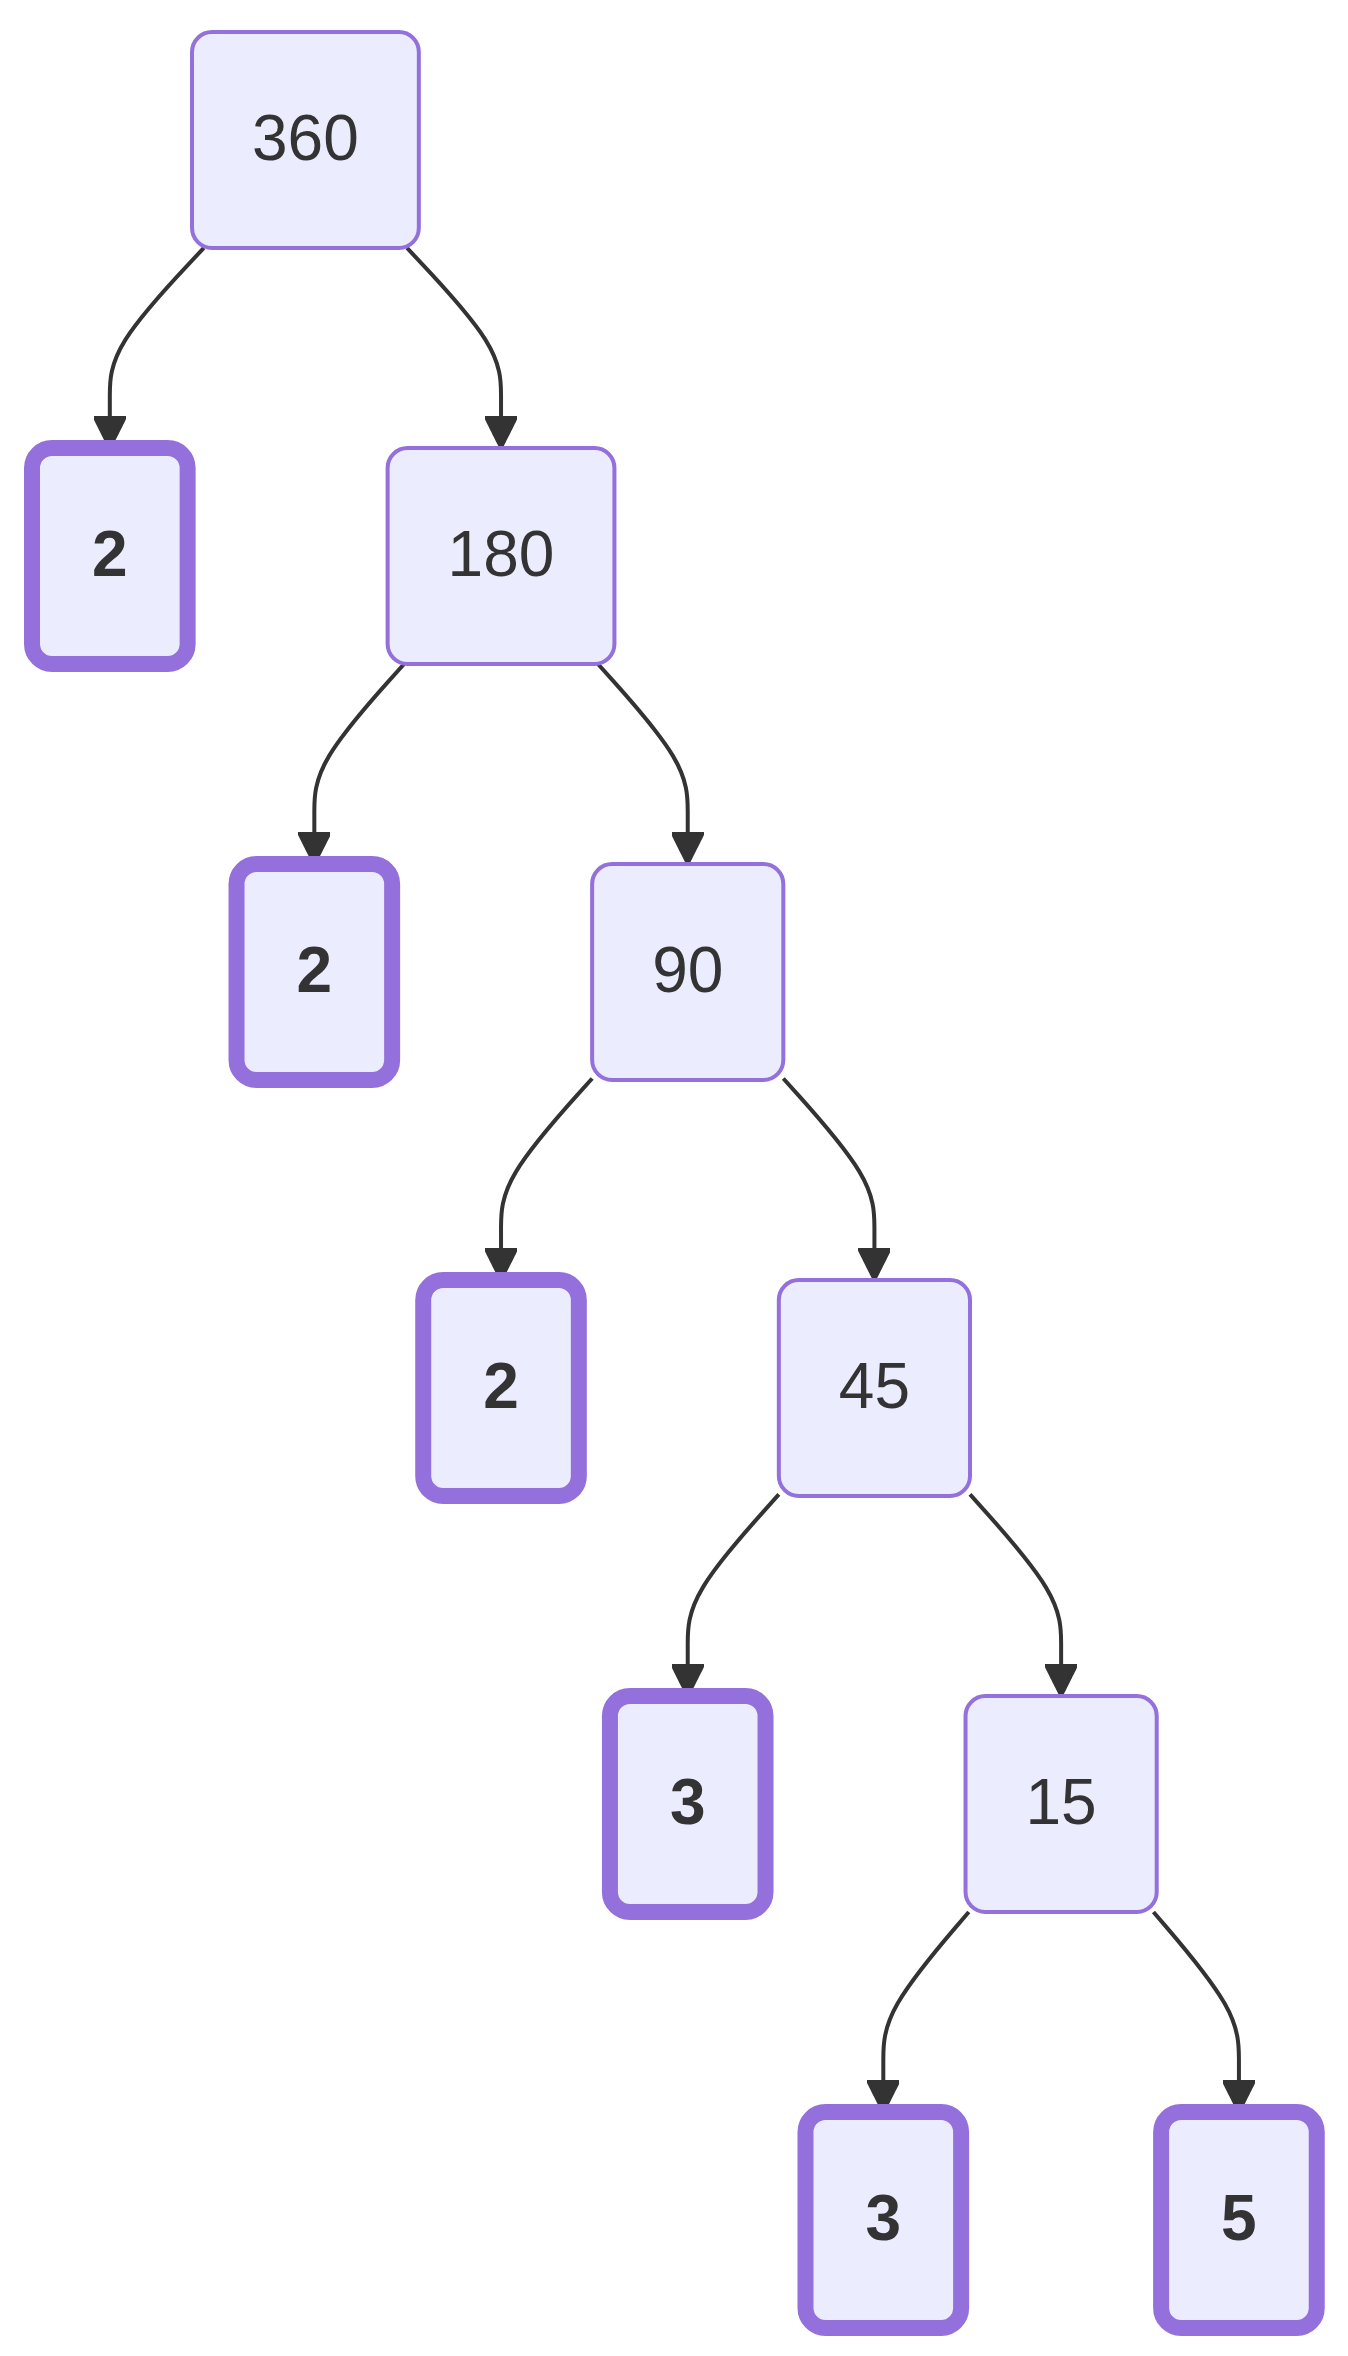
\includegraphics[width=3.51in,height=6.15in]{chapters/Unit_1/1.2_Factors_Multiples_&_Prime_Factorization_files/figure-latex/mermaid-figure-5.png}

When you divide by the smallest (or biggest) factors, the tree tends to
become deep. If you want smaller trees, you should start with factor
pairs that are closer together like we did with the first factor tree
for 360, splitting first with 18 and 20.

\end{tcolorbox}

\textbf{What About Negative Numbers?}

If the number is negative, factor out a -1 first. Here is one possible
factor tree for -24:

\phantomsection\label{mermaid-diagram}
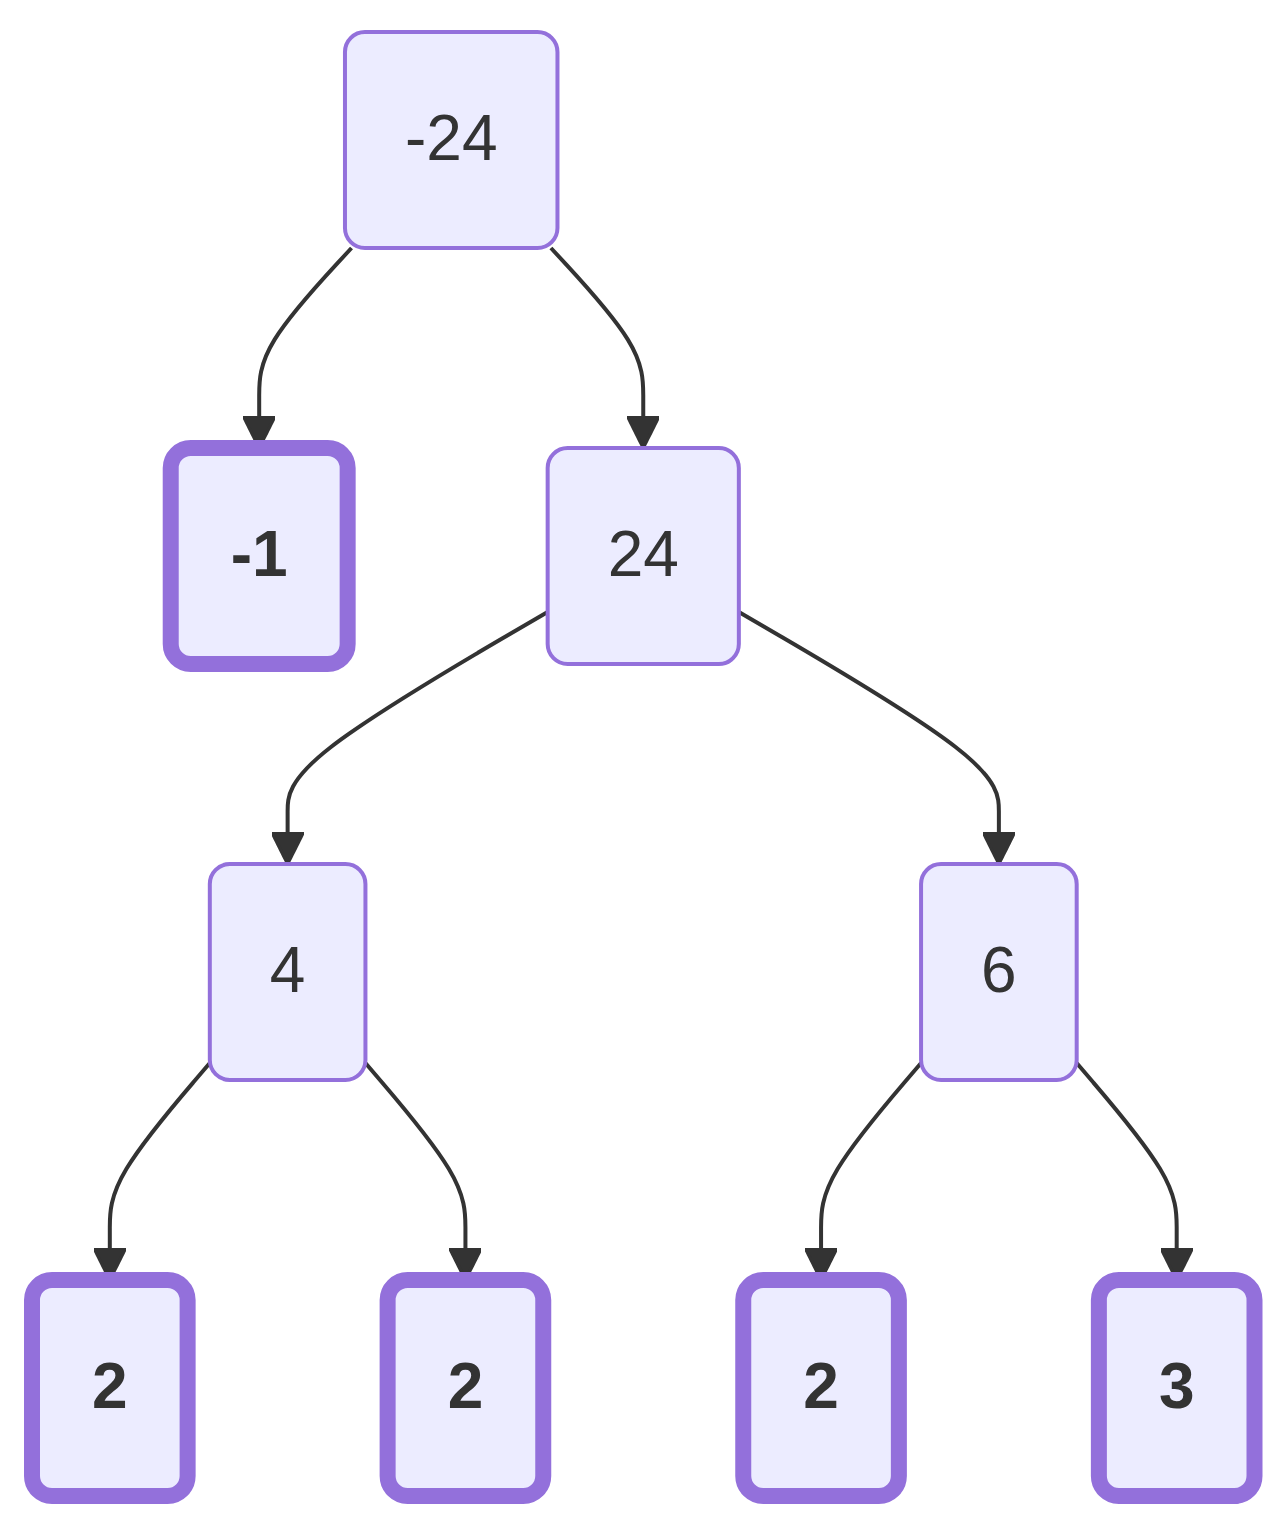
\includegraphics[width=3.35in,height=3.98in]{chapters/Unit_1/1.2_Factors_Multiples_&_Prime_Factorization_files/figure-latex/mermaid-figure-4.png}

So, the prime factorization of -24 is\ldots{}

\[-1 * 2^3 * 3 = -24\]

This will come in handy later when we factor algebraic
\href{./glossary.html\#glossary-expression}{expressions} like
\(-x^2 + 4x\). It's often helpful to pull out a negative first!

\textbf{Feeling overwhelmed?}

If you struggle to come up with the factors for a number, you should
check out the \href{./resources/Factor-Chart_noprimes.pdf}{factor chart}
in the resources section of this book. It shows all of the factor pairs
for many composite numbers!

I have only shown you 3 of the 60 unique factor trees for 360!

\section*{✍️ Practice On Your Own}\label{practice-on-your-own-1}
\addcontentsline{toc}{section}{✍️ Practice On Your Own}

\markright{✍️ Practice On Your Own}

\textbf{Factors \& Multiples}

\begin{enumerate}
\def\labelenumi{\arabic{enumi}.}
\item
  List all the factors of:

  \begin{enumerate}
  \def\labelenumii{\alph{enumii}.}
  \tightlist
  \item
    16
  \item
    18
  \item
    27
  \end{enumerate}
\item
  List the first 5 multiples of:

  \begin{enumerate}
  \def\labelenumii{\alph{enumii}.}
  \tightlist
  \item
    4
  \item
    9
  \item
    12
  \end{enumerate}
\end{enumerate}

\begin{center}\rule{0.5\linewidth}{0.5pt}\end{center}

\textbf{Prime or Composite?}

\begin{enumerate}
\def\labelenumi{\arabic{enumi}.}
\setcounter{enumi}{2}
\tightlist
\item
  Label each number as \textbf{prime}, \textbf{composite}, or
  \textbf{neither}:

  \begin{enumerate}
  \def\labelenumii{\alph{enumii}.}
  \tightlist
  \item
    7
  \item
    15
  \item
    1
  \item
    19
  \item
    21
  \end{enumerate}
\end{enumerate}

\begin{center}\rule{0.5\linewidth}{0.5pt}\end{center}

\textbf{Complete the Factor Tree}

\begin{enumerate}
\def\labelenumi{\arabic{enumi}.}
\setcounter{enumi}{3}
\item
  Fill in the missing numbers.

  \begin{enumerate}
  \def\labelenumii{\alph{enumii}.}
  \tightlist
  \item
  \end{enumerate}
\end{enumerate}

\begin{figure}

\centering{

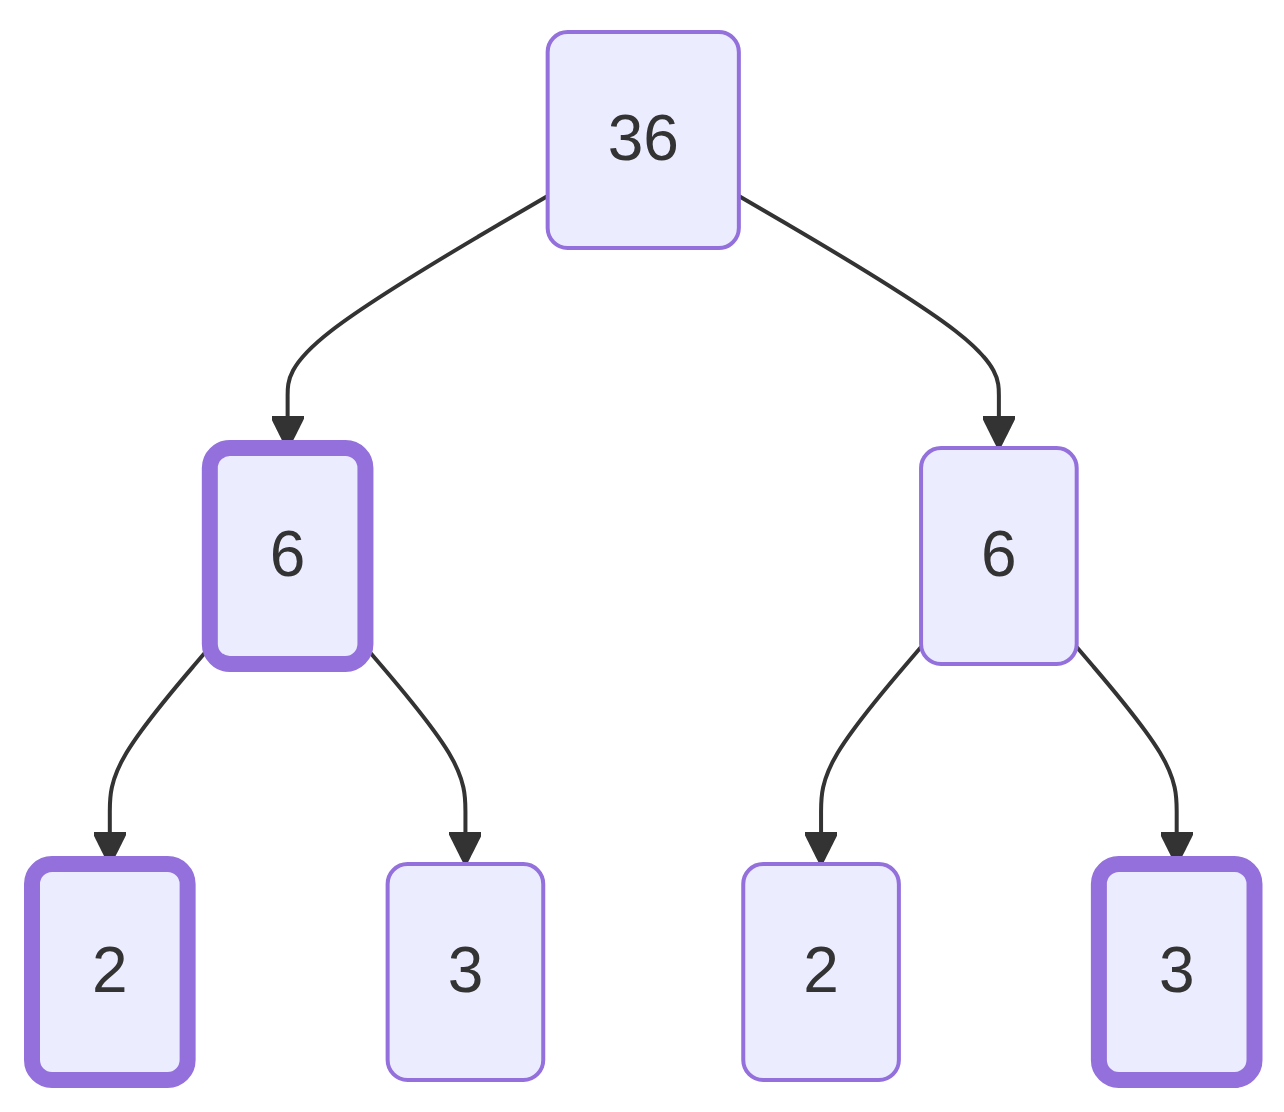
\includegraphics[width=3.35in,height=2.9in]{chapters/Unit_1/1.2_Factors_Multiples_&_Prime_Factorization_files/figure-latex/mermaid-figure-3.png}

}

\caption{\label{fig-mermaid-diagram}}

\end{figure}%

\begin{enumerate}
\def\labelenumi{\alph{enumi}.}
\setcounter{enumi}{1}
\tightlist
\item
\end{enumerate}

\begin{figure}

\centering{

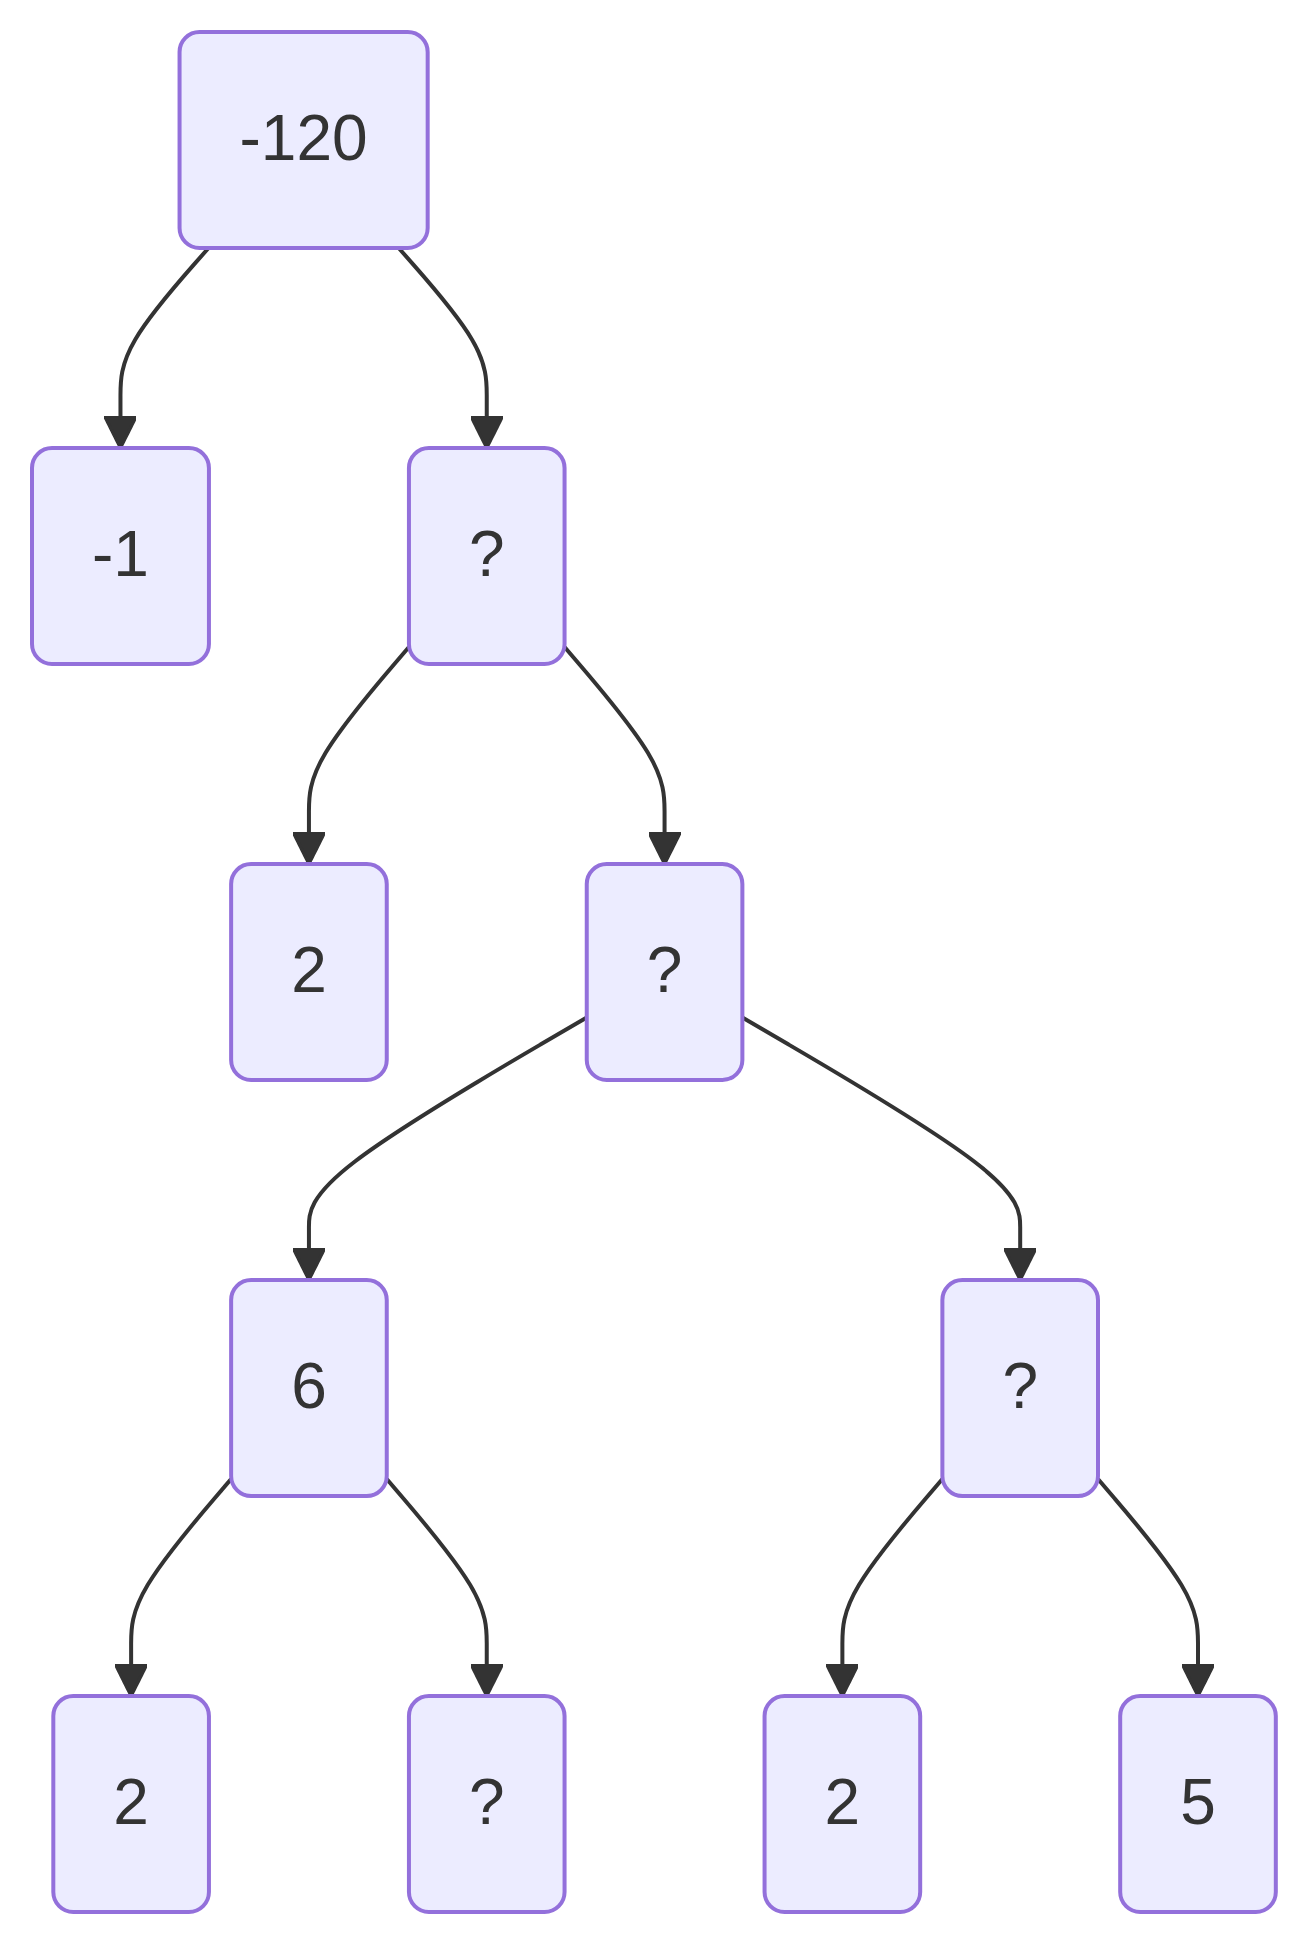
\includegraphics[width=3.41in,height=5.06in]{chapters/Unit_1/1.2_Factors_Multiples_&_Prime_Factorization_files/figure-latex/mermaid-figure-2.png}

}

\caption{\label{fig-mermaid-diagram}}

\end{figure}%

\begin{center}\rule{0.5\linewidth}{0.5pt}\end{center}

\textbf{Factor Trees \& Prime Factorization}

\begin{enumerate}
\def\labelenumi{\arabic{enumi}.}
\setcounter{enumi}{4}
\item
  Use a factor tree to find the prime factorization of:

  \begin{enumerate}
  \def\labelenumii{\alph{enumii}.}
  \tightlist
  \item
    24
  \item
    60
  \item
    100
  \item
    81
  \item
    72
  \end{enumerate}
\end{enumerate}

\begin{center}\rule{0.5\linewidth}{0.5pt}\end{center}

\textbf{Challenge}

\begin{enumerate}
\def\labelenumi{\arabic{enumi}.}
\setcounter{enumi}{5}
\tightlist
\item
  Can two different numbers have the same prime factorization? Why or
  why not?
\end{enumerate}

\begin{center}\rule{0.5\linewidth}{0.5pt}\end{center}

\textbf{Warm-Up}

\begin{enumerate}
\def\labelenumi{\arabic{enumi}.}
\item
  \textbf{5} (1, 36), (2, 18), (3, 12), (4,9), (6, 6)
\item
  8 (if we count zero, which is a whole number)
\item
  No, 13 is prime
\end{enumerate}

\begin{center}\rule{0.5\linewidth}{0.5pt}\end{center}

\textbf{Factors \& Multiples}

\begin{enumerate}
\def\labelenumi{\arabic{enumi}.}
\tightlist
\item
  \begin{enumerate}
  \def\labelenumii{\alph{enumii}.}
  \tightlist
  \item
    1, 2, 4, 8, 16
  \item
    1, 2, 3, 6, 9, 18
  \item
    1, 3, 9, 27
  \end{enumerate}
\item
  \begin{enumerate}
  \def\labelenumii{\alph{enumii}.}
  \tightlist
  \item
    4, 8, 12, 16, 20
  \item
    9, 18, 27, 36, 45
  \item
    12, 24, 36, 48, 60
  \end{enumerate}
\end{enumerate}

\begin{center}\rule{0.5\linewidth}{0.5pt}\end{center}

\textbf{Prime or Composite?}

\begin{enumerate}
\def\labelenumi{\arabic{enumi}.}
\setcounter{enumi}{2}
\tightlist
\item
  \begin{enumerate}
  \def\labelenumii{\alph{enumii}.}
  \tightlist
  \item
    Prime
  \item
    Composite
  \item
    Neither
  \item
    Prime
  \item
    Composite
  \end{enumerate}
\end{enumerate}

\begin{center}\rule{0.5\linewidth}{0.5pt}\end{center}

\textbf{Complete the Factor Tree}

\begin{enumerate}
\def\labelenumi{\arabic{enumi}.}
\setcounter{enumi}{3}
\tightlist
\item
\end{enumerate}

\begin{enumerate}
\def\labelenumi{\alph{enumi}.}
\tightlist
\item
\end{enumerate}

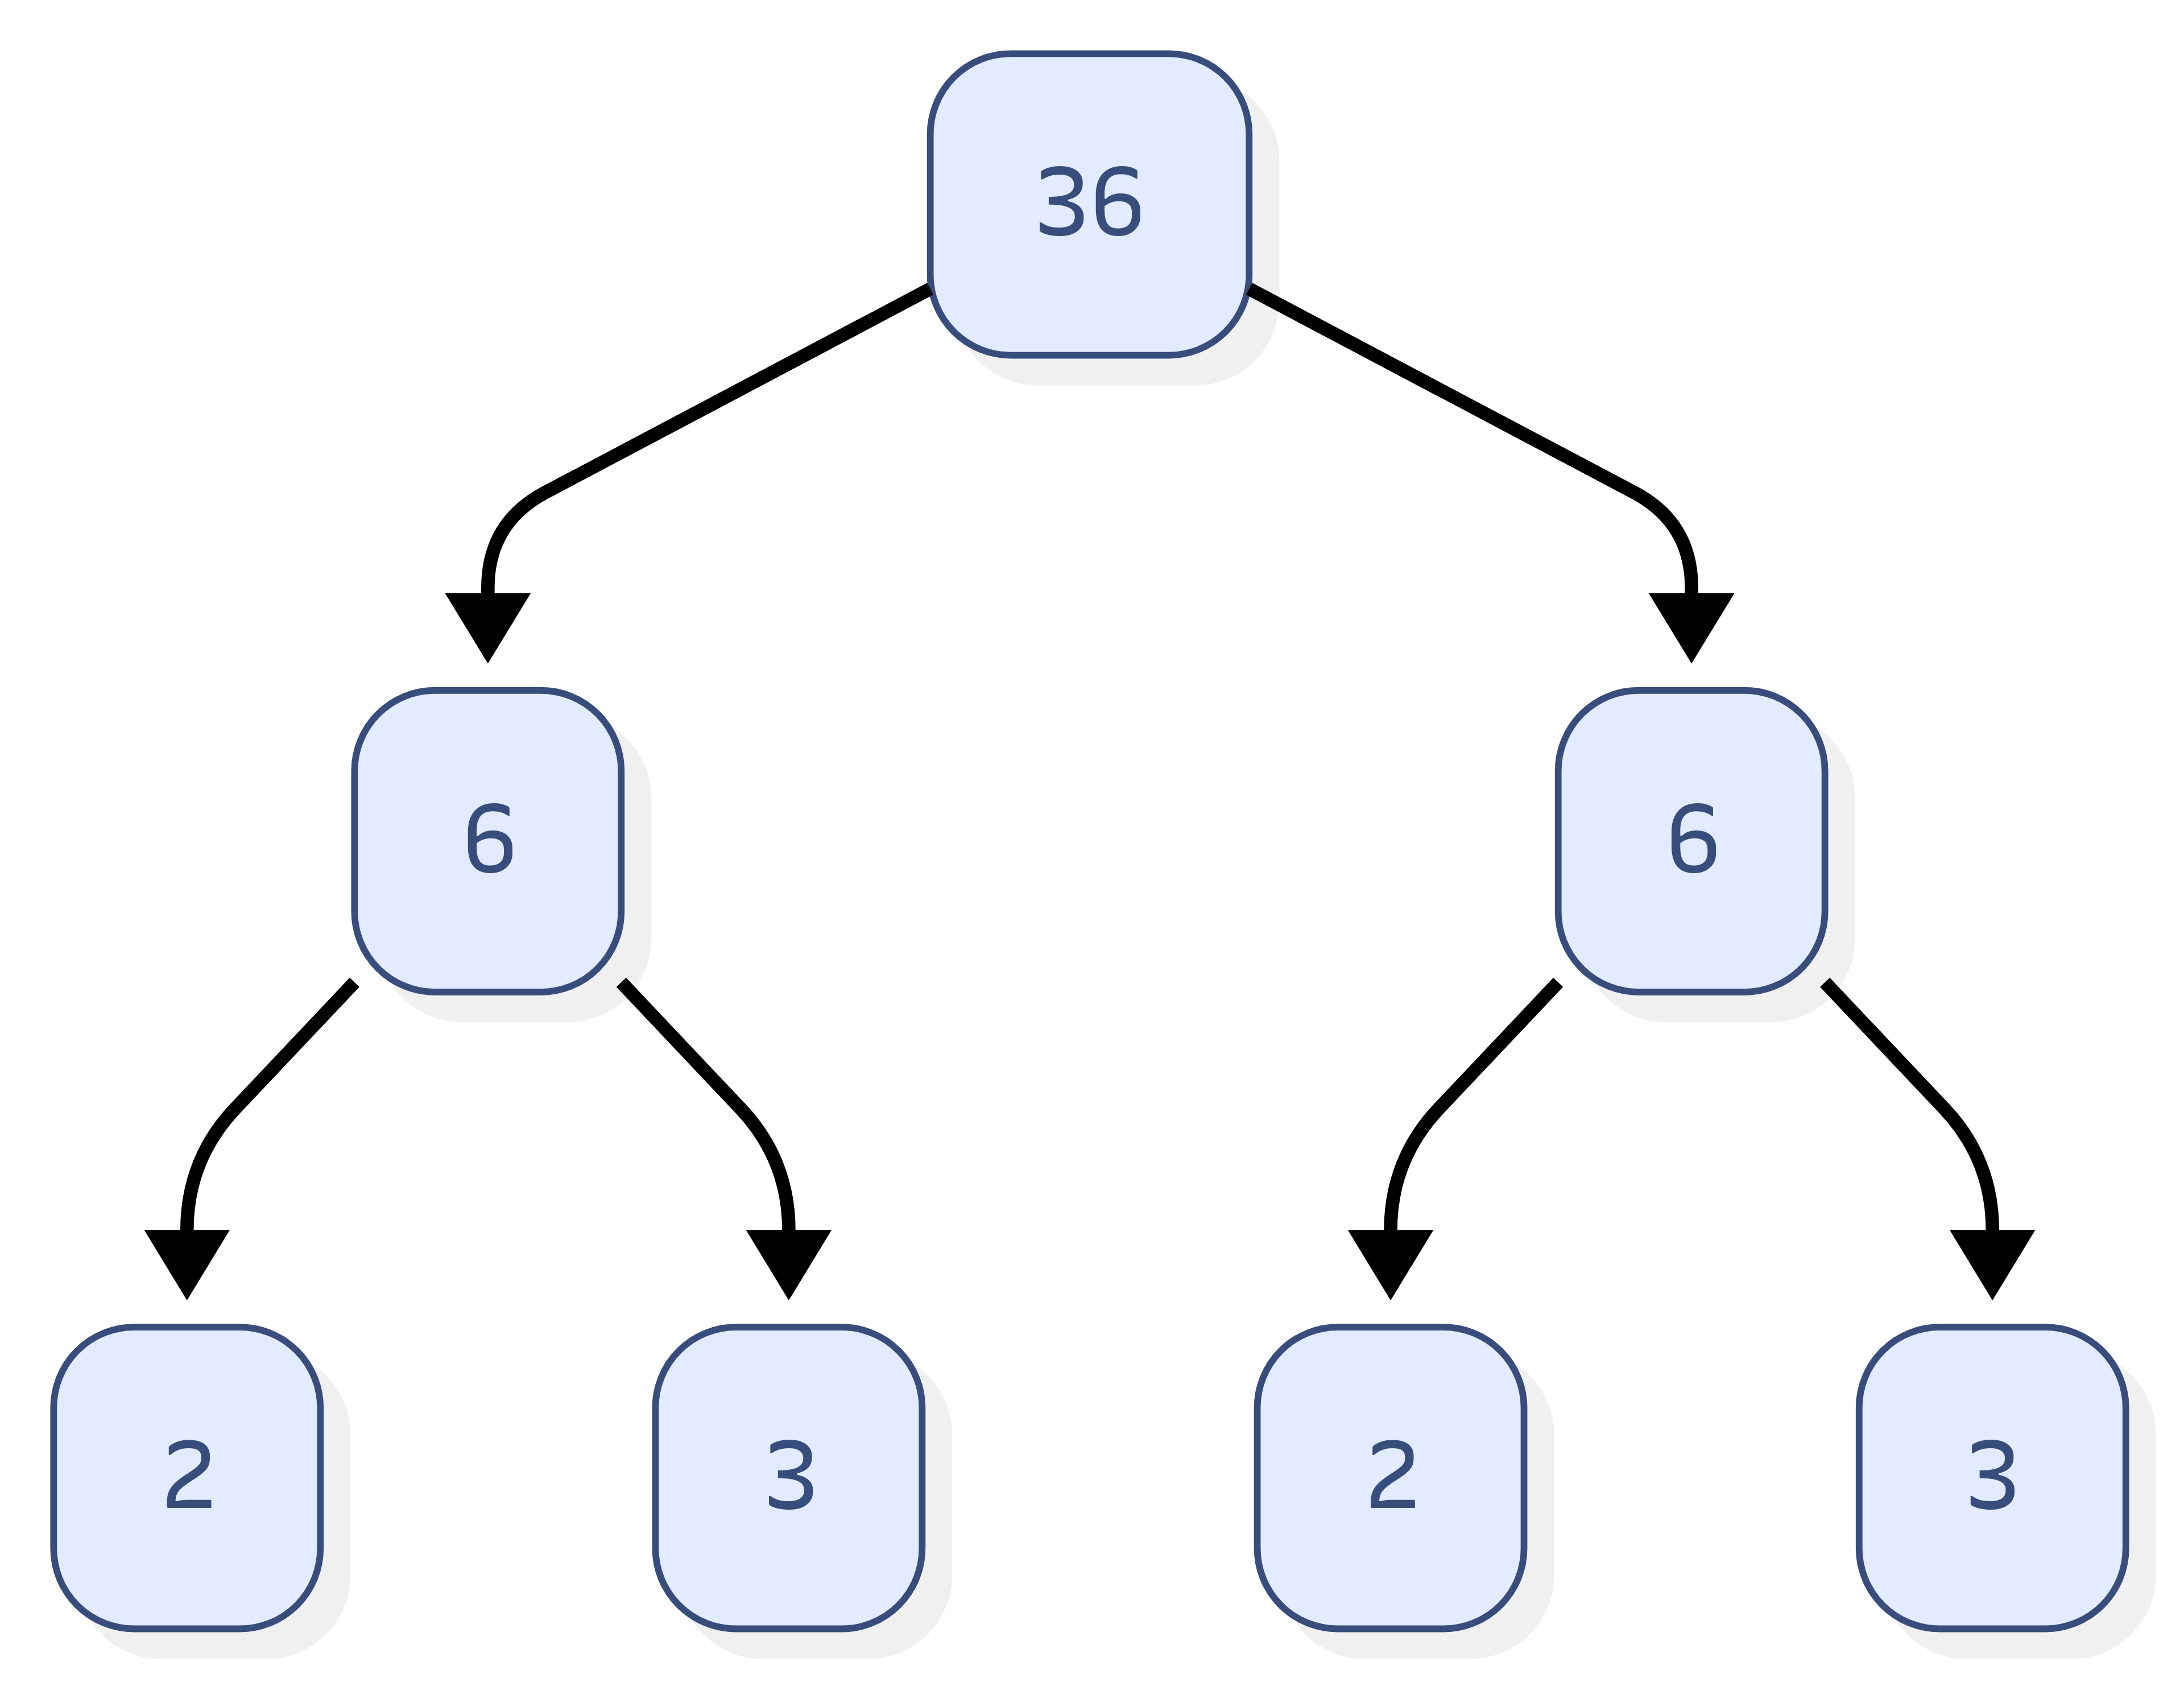
\includegraphics[width=\linewidth,height=2.08333in,keepaspectratio]{images/Unit_1/Lesson_2/lesson_1_2_4a.png}

\begin{enumerate}
\def\labelenumi{\alph{enumi}.}
\setcounter{enumi}{1}
\tightlist
\item
\end{enumerate}

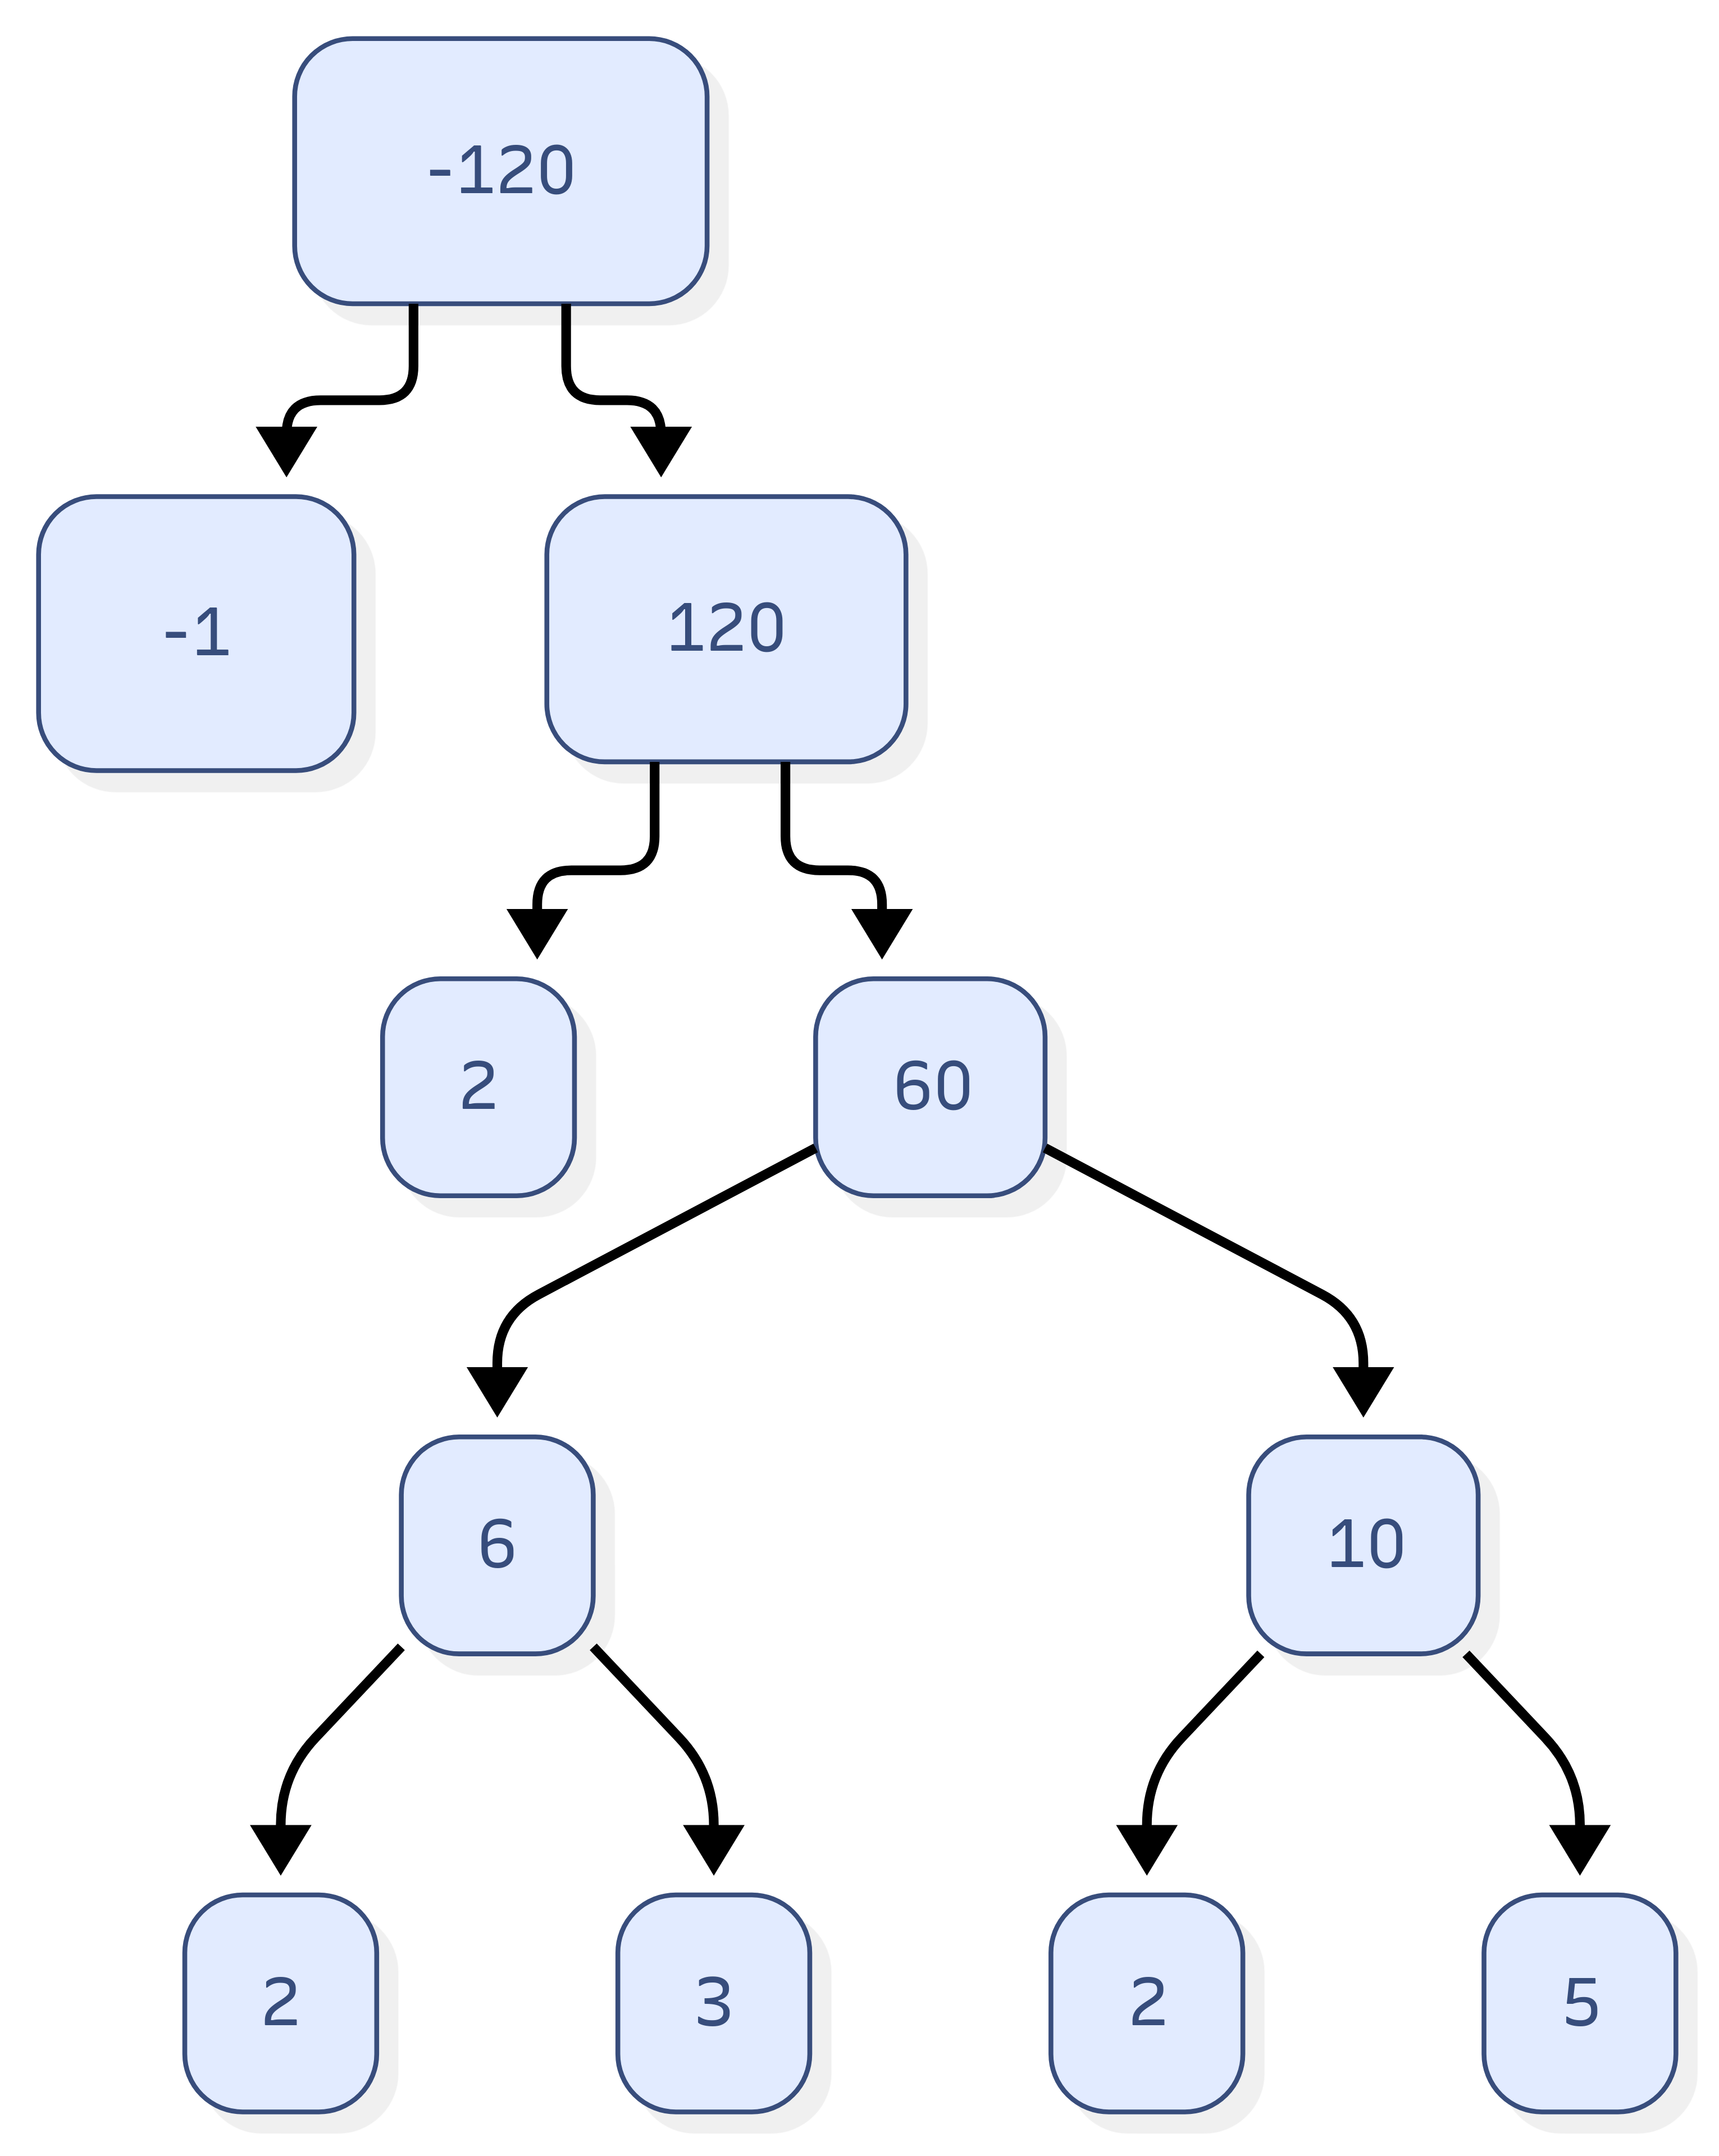
\includegraphics[width=\linewidth,height=3.125in,keepaspectratio]{images/Unit_1/Lesson_2/lesson_1_2_4b.png}

\begin{center}\rule{0.5\linewidth}{0.5pt}\end{center}

\textbf{Factor Trees and Prime Factorization}

\begin{enumerate}
\def\labelenumi{\arabic{enumi}.}
\setcounter{enumi}{4}
\tightlist
\item
  \begin{enumerate}
  \def\labelenumii{\alph{enumii}.}
  \tightlist
  \item
    2 × 2 × 2 × 3 = 2³ × 3
  \item
    2 × 2 × 3 × 5 = 2² × 3 × 5
  \item
    2 × 2 × 5 × 5 = 2² × 5²
  \item
    3 × 3 × 3 × 3 = 3⁴
  \item
    2 × 2 × 2 × 3 × 3 = 2³ × 3²
  \end{enumerate}
\end{enumerate}

\begin{center}\rule{0.5\linewidth}{0.5pt}\end{center}

\textbf{Challenge}

\begin{enumerate}
\def\labelenumi{\arabic{enumi}.}
\setcounter{enumi}{5}
\tightlist
\item
  No.~Each number has a \textbf{unique} prime factorization. This is
  called the \textbf{Fundamental Theorem of Arithmetic}.
\end{enumerate}

\chapter*{1.3 - GCF \& Simplifying
Fractions}\label{gcf-simplifying-fractions}
\addcontentsline{toc}{chapter}{1.3 - GCF \& Simplifying Fractions}

\markboth{1.3 - GCF \& Simplifying Fractions}{1.3 - GCF \& Simplifying
Fractions}

Suppose you're making snack packs and have 20 bags of chips and 35
cookies. What's the greatest number of identical packs you can make with
no leftovers? To figure that out, you'd use something called the
\href{./glossary.html\#glossary-greatest-common-factor}{greatest common factor}
(GCF).

In this lesson, you'll learn how to use
\href{./glossary.html\#glossary-prime-factorization}{prime factorization}
to find the GCF --- and how that can help you simplify
\href{./glossary.html\#glossary-fraction}{fractions}. Finding the GCF
makes numbers easier to work with, whether you're making snack packs or
solving math problems.

\begin{itemize}
\tightlist
\item[$\square$]
  I can find the GCF using factor trees
\item[$\square$]
  I can simplify fractions using the GCF
\item[$\square$]
  I can solve real-world problems using the GCF
\end{itemize}

\href{./glossary.html\#glossary-equivalent}{equivalent},
\href{./glossary.html\#glossary-greatest-common-factor}{greatest common factor},
\href{./glossary.html\#glossary-prime-factorization}{prime factorization},
\href{./glossary.html\#glossary-relatively-prime}{relatively prime},
\href{./glossary.html\#glossary-simplify}{simplify}

\begin{center}\rule{0.5\linewidth}{0.5pt}\end{center}

\section*{🔥 Warm-Up}\label{warm-up-2}
\addcontentsline{toc}{section}{🔥 Warm-Up}

\markright{🔥 Warm-Up}

\begin{enumerate}
\def\labelenumi{\arabic{enumi}.}
\item
  Which number do you \emph{think} has the most prime factors? What
  makes you think so?

  \begin{enumerate}
  \def\labelenumii{\alph{enumii}.}
  \item
    20
  \item
    30
  \item
    45
  \item
    53
  \end{enumerate}
\item
  What's the largest number that you think might divide \textbf{both} 12
  and 18 evenly?
\item
  Here are four fractions. Which one doesn't belong and why?

  \begin{enumerate}
  \def\labelenumii{\alph{enumii}.}
  \item
    \(\frac{12}{18}\)
  \item
    \(\frac{4}{9}\)
  \item
    \(\frac{2}{3}\)
  \item
    \(\frac{24}{36}\)
  \end{enumerate}
\end{enumerate}

\begin{center}\rule{0.5\linewidth}{0.5pt}\end{center}

\section*{👥 Learn Together}\label{learn-together-2}
\addcontentsline{toc}{section}{👥 Learn Together}

\markright{👥 Learn Together}

\subsection*{1.3.1 - Finding the GCF Using Factor
Trees}\label{finding-the-gcf-using-factor-trees}
\addcontentsline{toc}{subsection}{1.3.1 - Finding the GCF Using Factor
Trees}

To find the GCF, we can break numbers into their \textbf{prime factors}
using \href{./glossary.html\#glossary-factor-tree}{factor trees}.

Let's try it with 36 and 60:

\begin{figure}

\begin{minipage}{0.50\linewidth}

\phantomsection\label{mermaid-diagram}
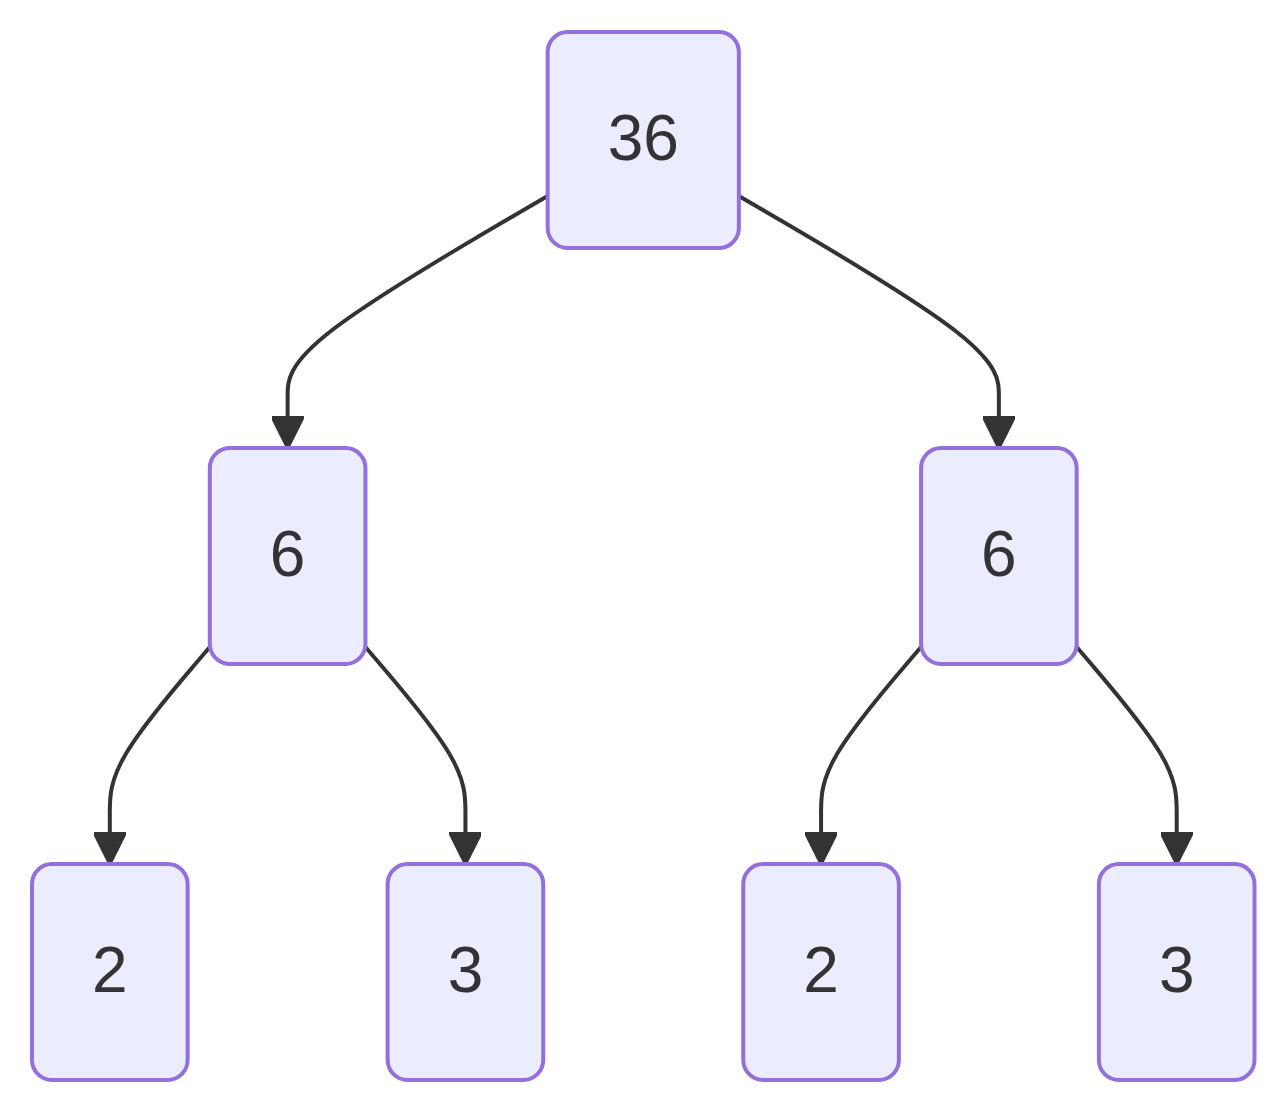
\includegraphics[width=3.35in,height=2.9in]{chapters/Unit_1/1.3_GCF_&_Simplifying_Fractions_files/figure-latex/mermaid-figure-6.png}

\end{minipage}%
%
\begin{minipage}{0.50\linewidth}

\phantomsection\label{mermaid-diagram}
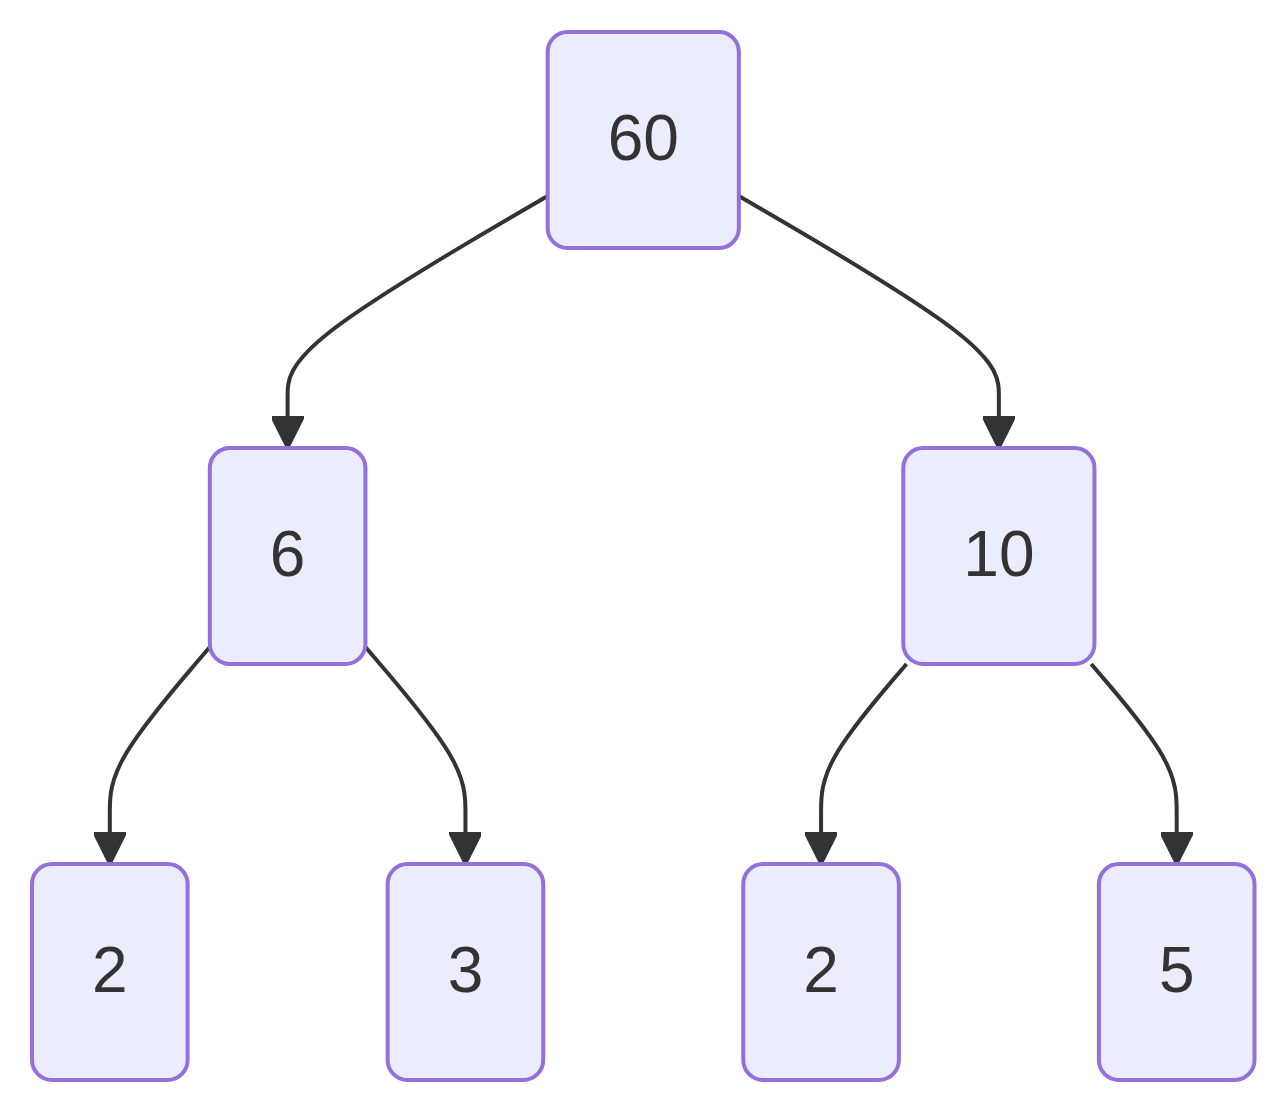
\includegraphics[width=3.35in,height=2.9in]{chapters/Unit_1/1.3_GCF_&_Simplifying_Fractions_files/figure-latex/mermaid-figure-21.png}

\end{minipage}%

\end{figure}%

Now that we have the factor trees, we can use them to easily find the
GCF by circling leaves that they both share.

\begin{figure}

\begin{minipage}{0.50\linewidth}

\phantomsection\label{mermaid-diagram}
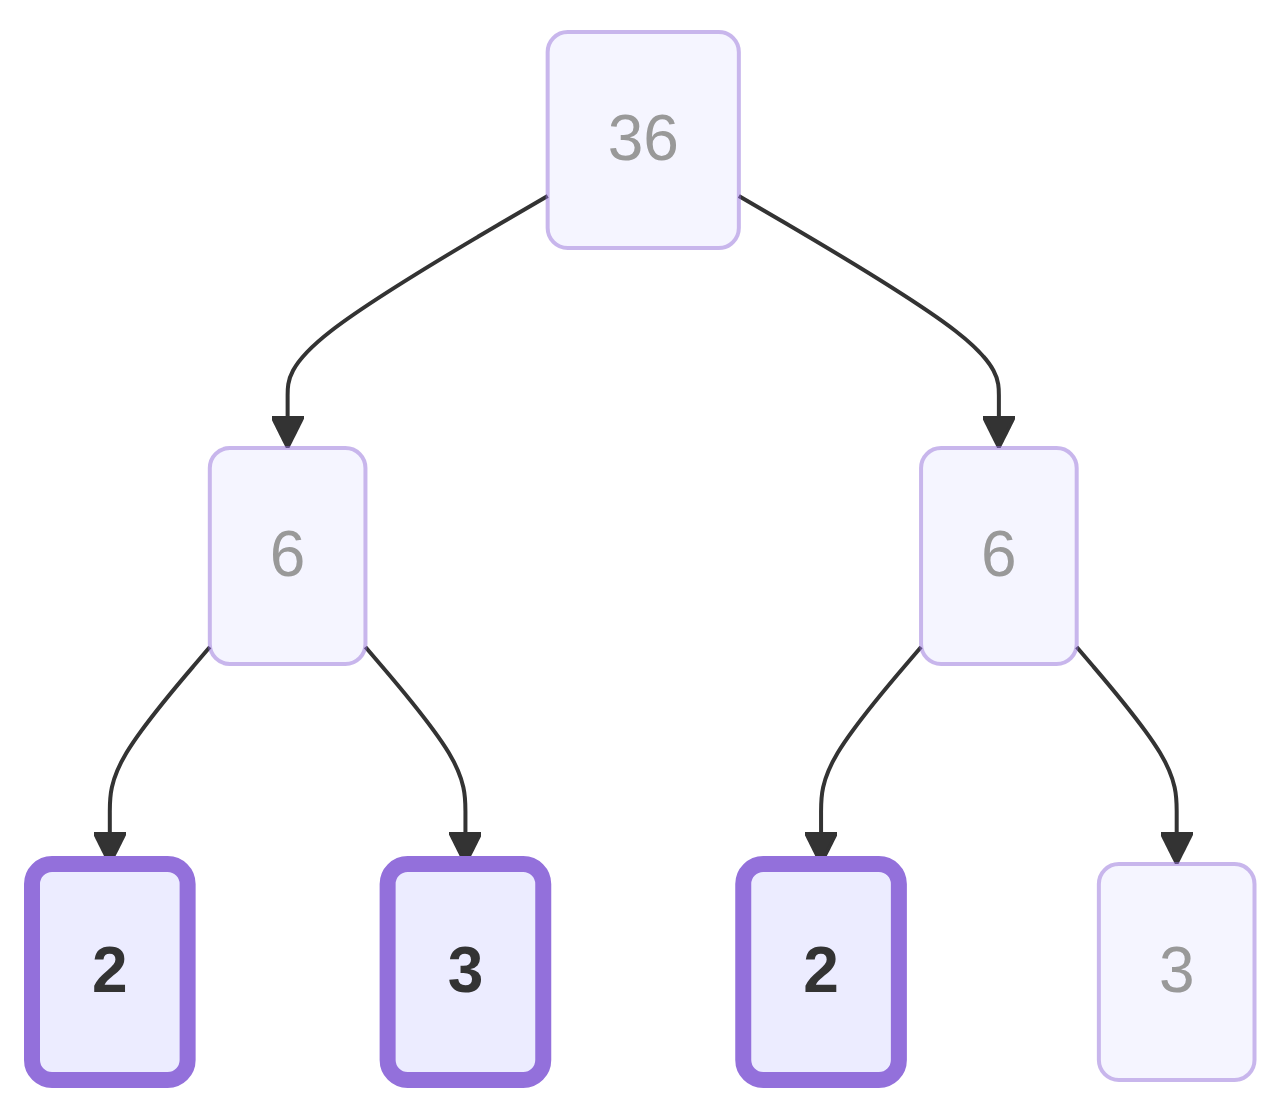
\includegraphics[width=3.35in,height=2.9in]{chapters/Unit_1/1.3_GCF_&_Simplifying_Fractions_files/figure-latex/mermaid-figure-20.png}

\end{minipage}%
%
\begin{minipage}{0.50\linewidth}

\phantomsection\label{mermaid-diagram}
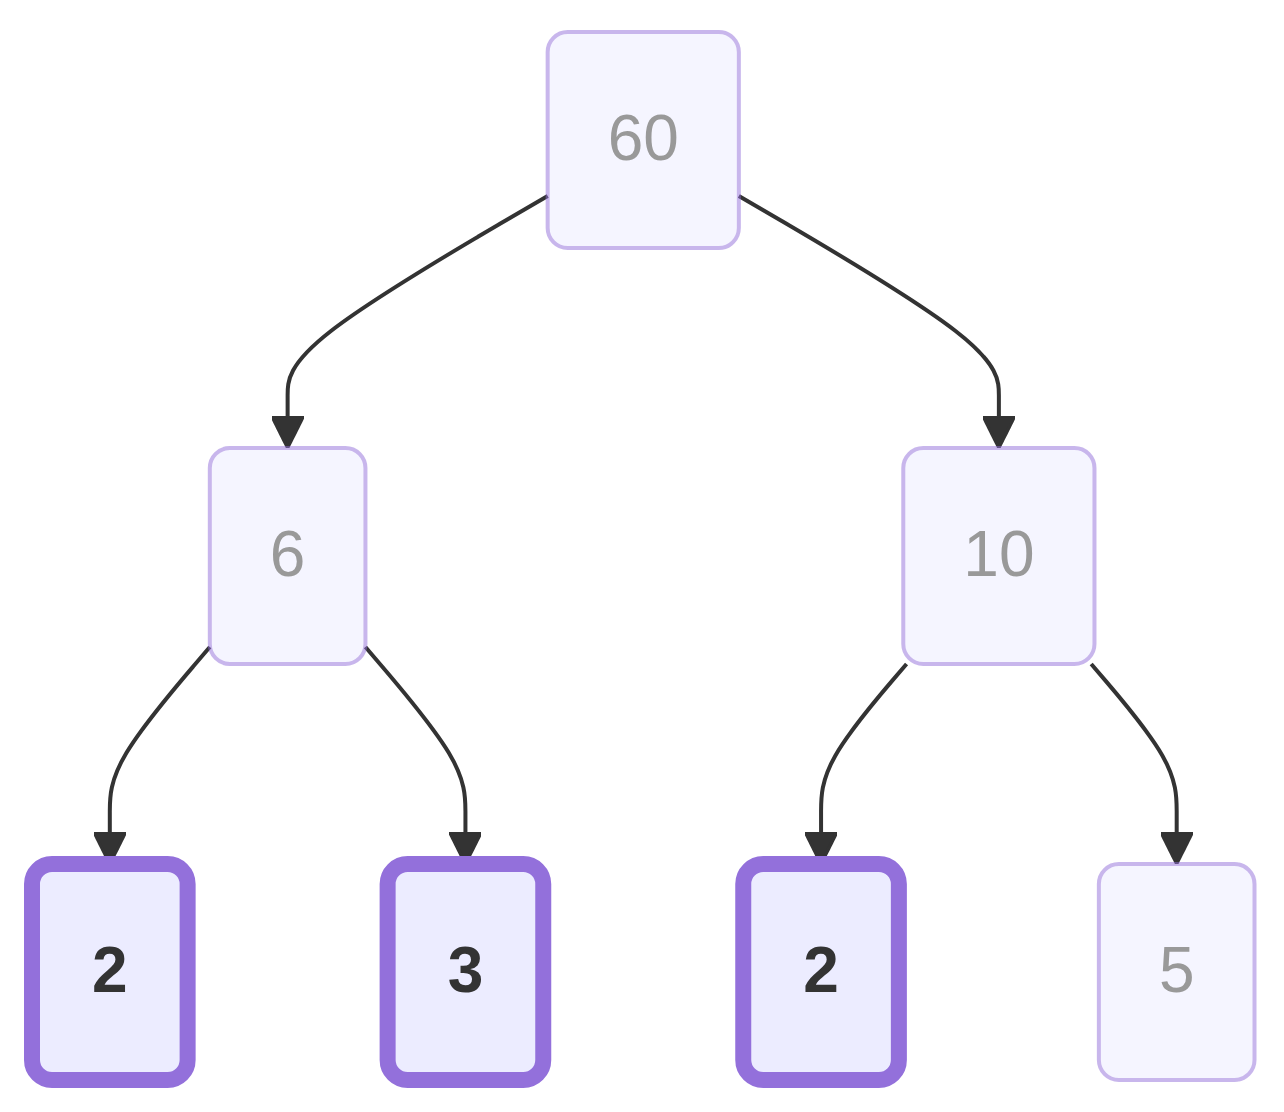
\includegraphics[width=3.35in,height=2.9in]{chapters/Unit_1/1.3_GCF_&_Simplifying_Fractions_files/figure-latex/mermaid-figure-19.png}

\end{minipage}%

\end{figure}%

The numbers 36 and 60 share two 2s and one 3. We find the GCF by
multiplying those shared factors. \[
2 * 2 * 3 = 12
\] The GCF for 36 and 60 is 12!

\begin{figure}

\begin{minipage}{0.50\linewidth}

\phantomsection\label{mermaid-diagram}
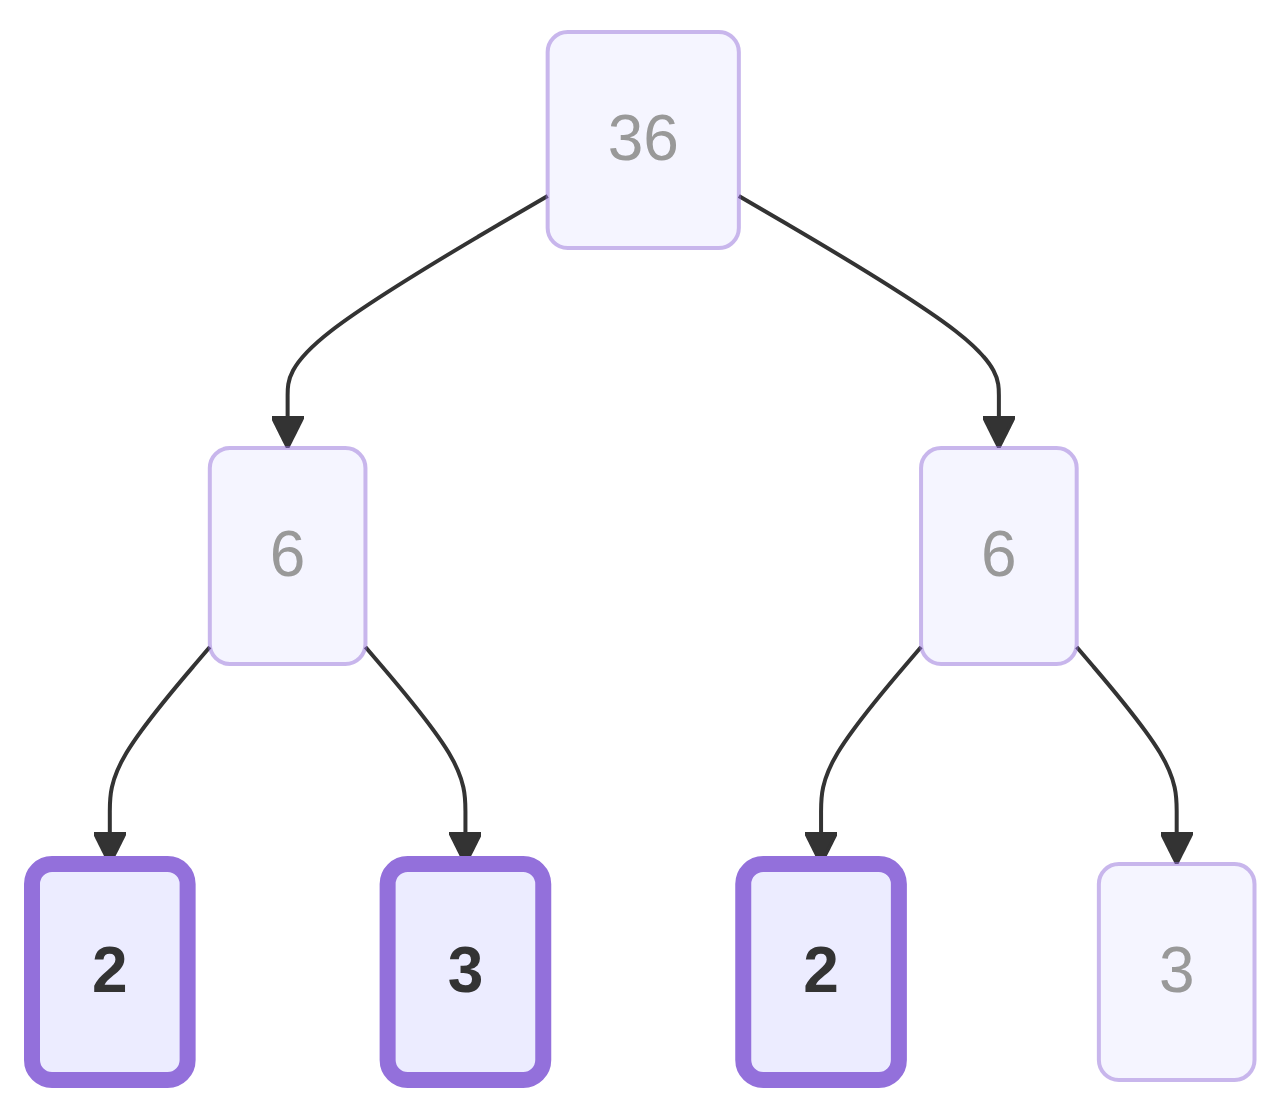
\includegraphics[width=1.96in,height=2.9in]{chapters/Unit_1/1.3_GCF_&_Simplifying_Fractions_files/figure-latex/mermaid-figure-18.png}

\end{minipage}%
%
\begin{minipage}{0.50\linewidth}

\phantomsection\label{mermaid-diagram}
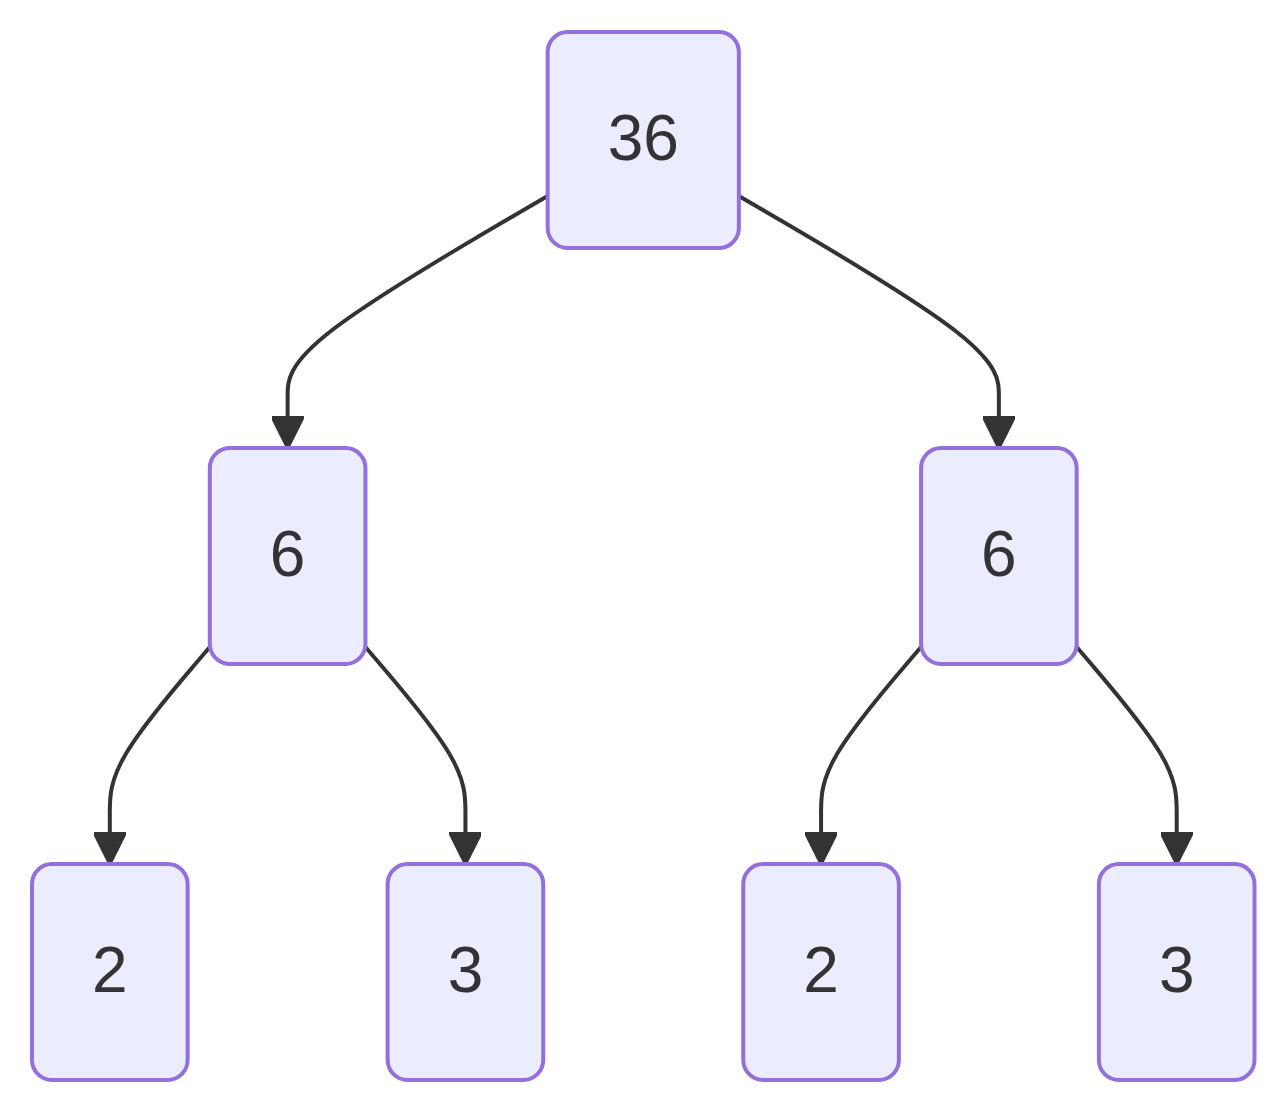
\includegraphics[width=3.35in,height=3.98in]{chapters/Unit_1/1.3_GCF_&_Simplifying_Fractions_files/figure-latex/mermaid-figure-17.png}

\end{minipage}%

\end{figure}%

Both 45 and 180 share two 3s and one 5. So the GCF for 45 and 180 is:

\[3 * 3 * 5 = 45\]

\begin{center}\rule{0.5\linewidth}{0.5pt}\end{center}

\subsection*{1.3.2 - Using Factor Trees to
Divide}\label{using-factor-trees-to-divide}
\addcontentsline{toc}{subsection}{1.3.2 - Using Factor Trees to Divide}

You might have noticed that we did not circle \textbf{all} of the prime
factors for 36 and 60 when finding their GCF of 12. What did we leave
behind and what does that mean?

\begin{figure}

\begin{minipage}{0.50\linewidth}

\phantomsection\label{mermaid-diagram}
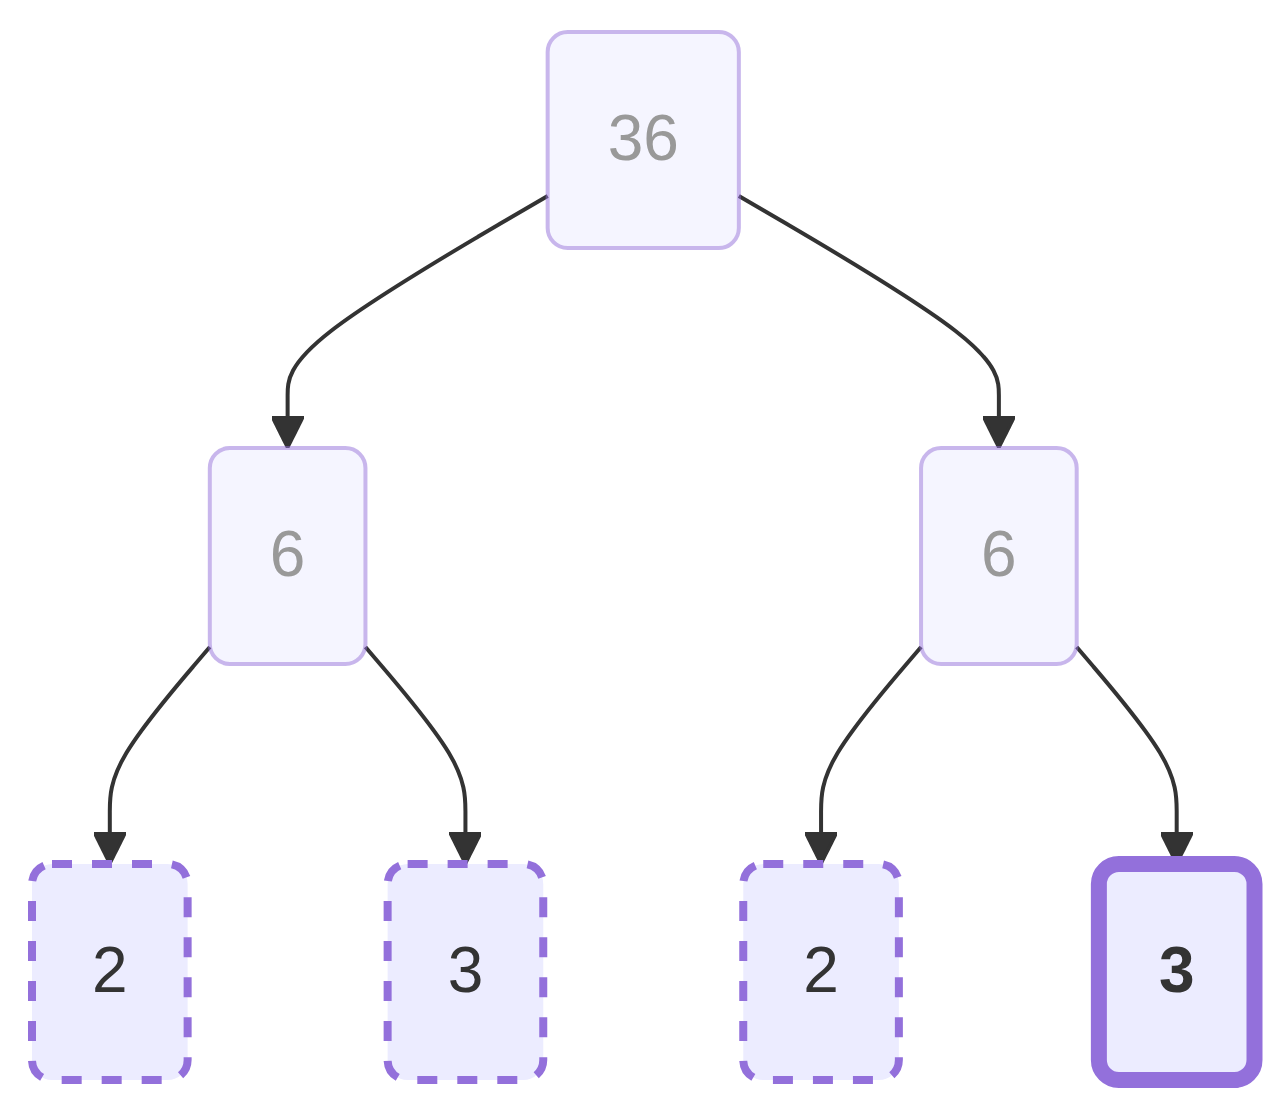
\includegraphics[width=3.35in,height=2.9in]{chapters/Unit_1/1.3_GCF_&_Simplifying_Fractions_files/figure-latex/mermaid-figure-16.png}

\end{minipage}%
%
\begin{minipage}{0.50\linewidth}

\phantomsection\label{mermaid-diagram}
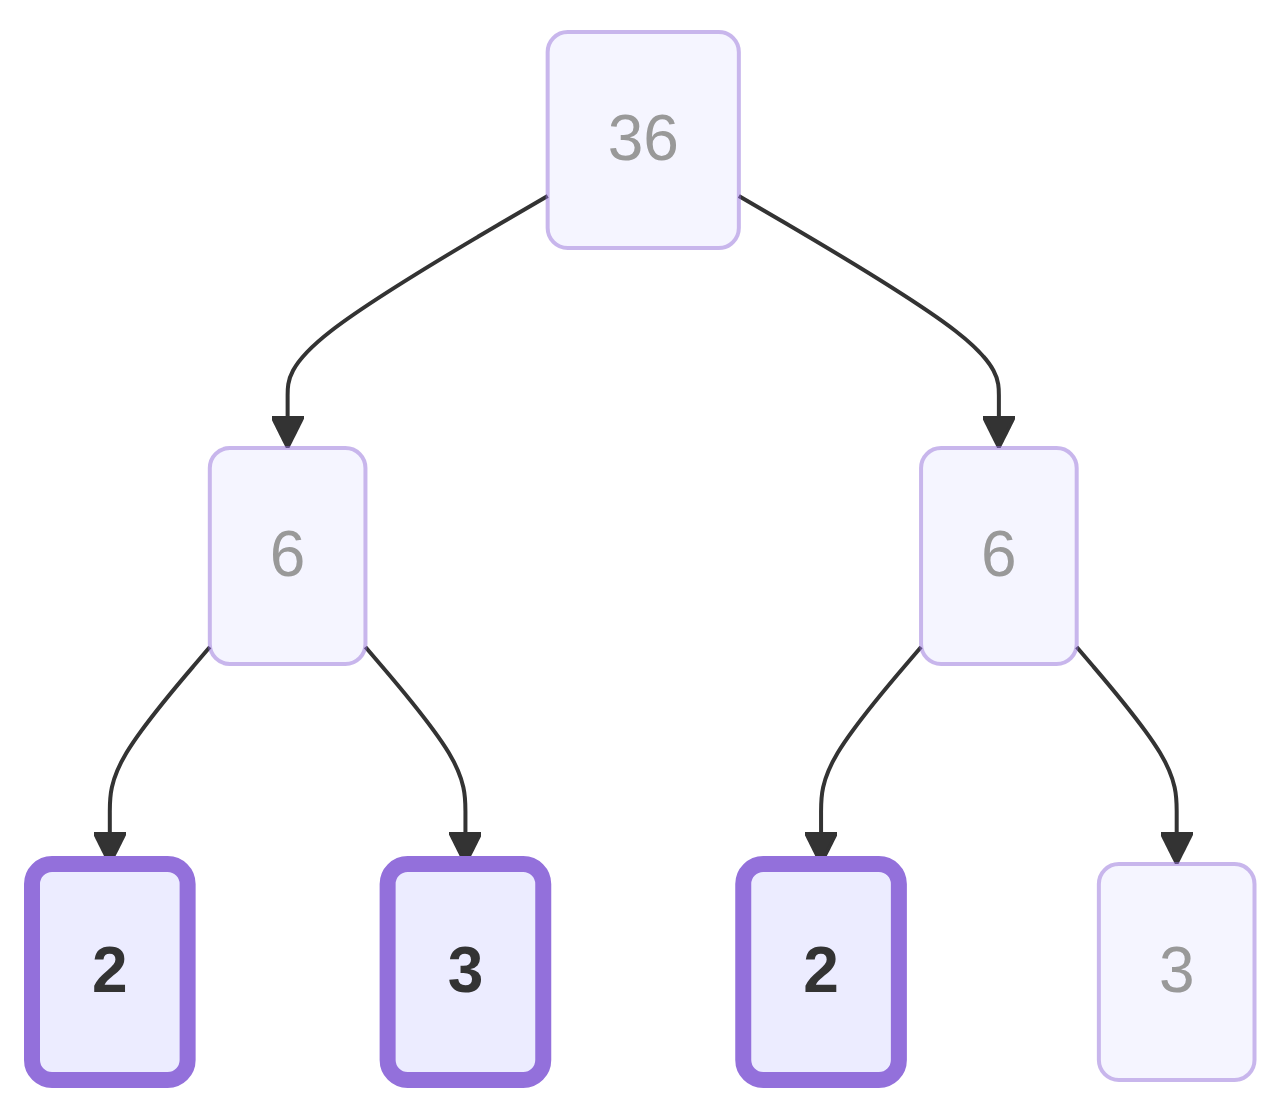
\includegraphics[width=3.35in,height=2.9in]{chapters/Unit_1/1.3_GCF_&_Simplifying_Fractions_files/figure-latex/mermaid-figure-15.png}

\end{minipage}%

\end{figure}%

For 36 we left behind a 3 and for 60 we left behind a 5. What this means
is that 36 ÷ 12 is 3 and 60 ÷ 12 is 5!''

\begin{center}\rule{0.5\linewidth}{0.5pt}\end{center}

\textbf{Let's try another one}

This time we will divide 90 by 15. Here are some factor trees to help
us.

\begin{figure}

\begin{minipage}{0.50\linewidth}

\phantomsection\label{mermaid-diagram}
\includegraphics[width=3.35in,height=2.9in]{chapters/Unit_1/1.3_GCF_&_Simplifying_Fractions_files/figure-latex/mermaid-figure-14.png}

\end{minipage}%
%
\begin{minipage}{0.50\linewidth}

\phantomsection\label{mermaid-diagram}
\includegraphics[width=1.5in,height=1.81in]{chapters/Unit_1/1.3_GCF_&_Simplifying_Fractions_files/figure-latex/mermaid-figure-13.png}

\end{minipage}%

\end{figure}%

The number 15 has prime factors 3 and 5. We can divide 90 by 15 by
crossing out those shared factors and multiplying what is left.

\includegraphics[width=3.35in,height=2.9in]{chapters/Unit_1/1.3_GCF_&_Simplifying_Fractions_files/figure-latex/mermaid-figure-12.png}

After crossing out 3 and 5 (the factors of 15) we are left with one 3
and one 2. This gives us\ldots{}

\[90 \div 15 = 3 * 2 = 6\]

\begin{enumerate}
\def\labelenumi{\arabic{enumi}.}
\tightlist
\item
  Find the factor trees for each number
\end{enumerate}

\begin{figure}

\begin{minipage}{0.50\linewidth}

\phantomsection\label{mermaid-diagram}
\includegraphics[width=5.2in,height=3.98in]{chapters/Unit_1/1.3_GCF_&_Simplifying_Fractions_files/figure-latex/mermaid-figure-11.png}

\end{minipage}%
%
\begin{minipage}{0.50\linewidth}

\phantomsection\label{mermaid-diagram}
\includegraphics[width=3.35in,height=2.9in]{chapters/Unit_1/1.3_GCF_&_Simplifying_Fractions_files/figure-latex/mermaid-figure-10.png}

\end{minipage}%

\end{figure}%

\begin{enumerate}
\def\labelenumi{\arabic{enumi}.}
\setcounter{enumi}{1}
\tightlist
\item
  Cross out the prime factors 480 shares with 60
\end{enumerate}

\includegraphics[width=5.2in,height=3.98in]{chapters/Unit_1/1.3_GCF_&_Simplifying_Fractions_files/figure-latex/mermaid-figure-9.png}

\begin{enumerate}
\def\labelenumi{\arabic{enumi}.}
\setcounter{enumi}{2}
\tightlist
\item
  Multiply the remaining prime factors to get the answer.
\end{enumerate}

\[2 * 2 * 2 = 8\]

\begin{center}\rule{0.5\linewidth}{0.5pt}\end{center}

\subsection*{1.3.3 - Simplifying Fractions with the
GCF}\label{simplifying-fractions-with-the-gcf}
\addcontentsline{toc}{subsection}{1.3.3 - Simplifying Fractions with the
GCF}

In the last section, dividing two numbers showed how to ``cancel out''
or eliminate shared factors. This is helpful when you want to
\href{./glossary.html\#glossary-simplify}{simplify} a fraction!

Simplifying a fraction means rewriting it in its
\href{./glossary.html\#glossary-simplest-form}{simplest form}. This
makes a fraction as ``small'' or ``basic'' as possible without changing
its value. To do that, we divide both the
\href{./glossary.html\#glossary-numerator}{numerator} and the
\href{./glossary.html\#glossary-denominator}{denominator} by their GCF.
When a fraction is in its simplest form, the numerator and denominator
don't share any factors other than 1.

\begin{center}\rule{0.5\linewidth}{0.5pt}\end{center}

Let's go back to one we've already seen:

\[
\frac{36}{60}
\]

We found earlier that the GCF of 36 and 60 is 12. So to simplify, we
divide both the numerator and denominator by 12:

\[
\frac{36 \div 12}{60 \div 12} = \frac{3}{5}
\]

This is just like the division you saw in the factor trees. We canceled
out the factors they both had --- two 2s and one 3 --- and kept what was
left.

\begin{center}\rule{0.5\linewidth}{0.5pt}\end{center}

\textbf{Here's another:}

\[
\frac{90}{15}
\]

We know that 15 is the GCF of 90 and 15. So:

\[
\frac{90 \div 15}{15 \div 15} = \frac{6}{1} = 6
\]

This tells us the fraction \(\frac{90}{15}\) is just another way to
write the number 6.

\begin{center}\rule{0.5\linewidth}{0.5pt}\end{center}

\textbf{In other words:}

\begin{quote}
Simplifying a fraction is just dividing the numerator and denominator by
their greatest common factor.
\end{quote}

Factor trees help you \emph{see} why this works by breaking the numbers
into their building blocks.

If the numerator and denominator of a fraction share no common factors
(besides 1) the two numbers are called
\href{./glossary.html\#glossary-relatively-prime}{relatively prime}. In
this case, the fraction cannot be simplified.

\textbf{Example:}

Simplify \(\frac{9}{38}\).

\begin{figure}

\begin{minipage}{0.50\linewidth}

\phantomsection\label{mermaid-diagram}
\includegraphics[width=1.5in,height=1.81in]{chapters/Unit_1/1.3_GCF_&_Simplifying_Fractions_files/figure-latex/mermaid-figure-8.png}

\end{minipage}%
%
\begin{minipage}{0.50\linewidth}

\phantomsection\label{mermaid-diagram}
\includegraphics[width=1.59in,height=1.81in]{chapters/Unit_1/1.3_GCF_&_Simplifying_Fractions_files/figure-latex/mermaid-figure-7.png}

\end{minipage}%

\end{figure}%

Since 9 and 38 share no factors, \(\frac{9}{38}\) is already in simplest
form.

The GCF of 30 and 90 is 30. \[
\frac{30}{90} = \frac{30 \div 30}{90 \div 30} = \frac{1}{3}
\]

\begin{center}\rule{0.5\linewidth}{0.5pt}\end{center}

\subsection*{1.3.4 -- Application: Simplifying with
Recipes}\label{application-simplifying-with-recipes}
\addcontentsline{toc}{subsection}{1.3.4 -- Application: Simplifying with
Recipes}

Imagine you're following a recipe that makes a giant batch of cookies
--- way more than you need. You decide to cut the recipe down to a
smaller size, but the measurements are a little awkward.

Here's what the recipe says:

\begin{itemize}
\item
  36 cups of flour
\item
  60 cups of sugar
\end{itemize}

You don't want to bake that much --- just a smaller, simpler version of
the same cookie. But how do you shrink the recipe without changing how
the cookies taste?

Let's treat the ingredients like a
\href{./glossary.html\#glossary-ratio}{ratio}:

\[
\frac{36 \text{ cups of flour}}{60 \text{ cups of sugar}}
\]

This \textbf{ratio} tells us how much flour to use per amount of sugar.
But the numbers are too big --- and a little messy.

Just like with fractions, we can simplify this ratio by dividing both
parts by their GCF. We already know the GCF of 36 and 60 is 12.

\[
\frac{36 \div 12}{60 \div 12} = \frac{3}{5}
\]

So for every 3 cups of flour, you need 5 cups of sugar.

Now you can make a smaller batch that keeps the same balance by finding
\href{./glossary.html\#glossary-multiple}{multiples} of the
\href{./glossary.html\#glossary-numerator}{numerator} and
\href{./glossary.html\#glossary-denominator}{denominator}. For example:

\begin{itemize}
\item
  3 cups of flour
\item
  5 cups of sugar
\end{itemize}

Or double that:

\begin{itemize}
\item
  6 cups of flour
\item
  10 cups of sugar
\end{itemize}

Simplifying the original recipe helped you find a cleaner ratio --- one
that's easier to scale up or down, depending on how many cookies you
want.

Simplifying isn't just a math trick --- it helps you work with numbers
more easily in the real world. Whether you're adjusting recipes, mixing
paint, or scaling blueprints, understanding fractions and simplifying
them makes life easier.

\begin{center}\rule{0.5\linewidth}{0.5pt}\end{center}

\section*{✍️ Practice On Your Own}\label{practice-on-your-own-2}
\addcontentsline{toc}{section}{✍️ Practice On Your Own}

\markright{✍️ Practice On Your Own}

\textbf{GCF Practice}

\begin{enumerate}
\def\labelenumi{\arabic{enumi}.}
\item
  Find the greatest common factor (GCF) of each pair:

  \begin{enumerate}
  \def\labelenumii{\alph{enumii}.}
  \tightlist
  \item
    20 and 30
  \item
    36 and 45
  \item
    18 and 48
  \item
    30 and 42
  \item
    50 and 65
  \item
    72 and 90
  \item
    81 and 108
  \end{enumerate}
\item
  Two numbers have a GCF of 6. One of the numbers is 18. What could the
  other number be? Give two possible answers.
\item
  Two numbers have a GCF of 1. What does that mean? Give an example.
\end{enumerate}

\begin{center}\rule{0.5\linewidth}{0.5pt}\end{center}

\textbf{Simplifying Fractions}

\begin{enumerate}
\def\labelenumi{\arabic{enumi}.}
\setcounter{enumi}{3}
\item
  Simplify each fraction:

  \begin{enumerate}
  \def\labelenumii{\alph{enumii}.}
  \tightlist
  \item
    \(\frac{18}{27}\)
  \item
    \(\frac{50}{100}\)
  \item
    \(\frac{14}{49}\)
  \item
    \(\frac{48}{60}\)
  \item
    \(\frac{84}{36}\)
  \item
    \(\frac{75}{90}\)
  \item
    \(\frac{99}{121}\)
  \item
    \(\frac{16}{40}\)
  \end{enumerate}
\item
  Can a fraction be simplified if the GCF is 1? Explain your answer and
  give an example.
\end{enumerate}

\begin{center}\rule{0.5\linewidth}{0.5pt}\end{center}

\textbf{Word Problems}

\begin{enumerate}
\def\labelenumi{\arabic{enumi}.}
\setcounter{enumi}{5}
\item
  You have 72 juice boxes and 60 cookies. You want to make snack packs
  with the \textbf{same number} of each. You must use \textbf{all} the
  items.

  \begin{enumerate}
  \def\labelenumii{\alph{enumii}.}
  \tightlist
  \item
    What's the greatest number of snack packs you can make?
  \item
    How many juice boxes and cookies go in each pack?
  \end{enumerate}
\item
  A store is making bundles using 108 pairs of socks and 144 shirts.
  Each bundle must have the same number of socks and the same number of
  shirts. There should be no leftovers.

  \begin{enumerate}
  \def\labelenumii{\alph{enumii}.}
  \tightlist
  \item
    What is the greatest number of bundles they can make?
  \item
    How many socks and shirts will go in each bundle?
  \end{enumerate}
\item
  A painter mixes 84 ounces of red paint and 36 ounces of blue paint. He
  wants to pour the paint into small jars that are all the same. Each
  jar must have the same mix of red and blue paint.

  \begin{enumerate}
  \def\labelenumii{\alph{enumii}.}
  \tightlist
  \item
    What is the greatest number of jars he can make with no paint left
    over?
  \item
    How many ounces of red and blue paint will go in each jar?
  \end{enumerate}
\end{enumerate}

\begin{center}\rule{0.5\linewidth}{0.5pt}\end{center}

\textbf{Challenge Problems}

\begin{enumerate}
\def\labelenumi{\arabic{enumi}.}
\setcounter{enumi}{8}
\item
  Two numbers multiply to make 180. Their GCF is 6. What could the
  numbers be?
\item
  A teacher has 150 pencils and 100 pens. She will make gift bags that
  all have the same number of pencils and the same number of pens. Each
  bag must have \textbf{2 more pencils than pens}. She will use
  \textbf{all} the items. How many bags can she make, and what goes in
  each bag?
\end{enumerate}

\begin{center}\rule{0.5\linewidth}{0.5pt}\end{center}

\textbf{Warm-Up}

\begin{enumerate}
\def\labelenumi{\arabic{enumi}.}
\item
  Which number do you \emph{think} has the most prime factors? What
  makes you think so?

  \begin{enumerate}
  \def\labelenumii{\alph{enumii}.}
  \item
    20
  \item
    30
  \item
    45
  \item
    53
  \end{enumerate}
\item
  What's the largest number that you think might divide \textbf{both} 12
  and 18 evenly?
\item
  Here are four fractions. Which one doesn't belong and why?

  \begin{enumerate}
  \def\labelenumii{\alph{enumii}.}
  \item
    \(\frac{12}{18}\)
  \item
    \(\frac{4}{9}\)
  \item
    \(\frac{2}{3}\)
  \item
    \(\frac{24}{36}\)
  \end{enumerate}
\end{enumerate}

\begin{center}\rule{0.5\linewidth}{0.5pt}\end{center}

\textbf{GCF Practice}

\begin{enumerate}
\def\labelenumi{\arabic{enumi}.}
\item
  \begin{enumerate}
  \def\labelenumii{\alph{enumii}.}
  \tightlist
  \item
    10
  \item
    9
  \item
    6
  \item
    6
  \item
    5
  \item
    18
  \item
    27
  \end{enumerate}
\item
  Examples: 30 or 42
\item
  The numbers are
  \href{./glossary.html\#glossary-relatively-prime}{relatively prime}.
  For example: 8 and 15.
\end{enumerate}

\begin{center}\rule{0.5\linewidth}{0.5pt}\end{center}

\textbf{Simplifying Fractions}

\begin{enumerate}
\def\labelenumi{\arabic{enumi}.}
\setcounter{enumi}{3}
\tightlist
\item
  \begin{enumerate}
  \def\labelenumii{\alph{enumii}.}
  \tightlist
  \item
    \(\frac{2}{3}\)
  \item
    \(\frac{1}{2}\)
  \item
    \(\frac{2}{7}\)
  \item
    \(\frac{4}{5}\)
  \item
    \(\frac{7}{3}\)
  \item
    \(\frac{5}{6}\)
  \item
    \(\frac{9}{11}\)
  \item
    \(\frac{2}{5}\)
  \end{enumerate}
\item
  No.~The numerator and denominator are relatively prime and so nothing
  can cancel out.
\end{enumerate}

\begin{center}\rule{0.5\linewidth}{0.5pt}\end{center}

\textbf{Word Problems}

\begin{enumerate}
\def\labelenumi{\arabic{enumi}.}
\setcounter{enumi}{5}
\tightlist
\item
  \begin{enumerate}
  \def\labelenumii{\alph{enumii}.}
  \tightlist
  \item
    12 snack packs
  \item
    6 juice boxes and 5 cookies
  \end{enumerate}
\item
  \begin{enumerate}
  \def\labelenumii{\alph{enumii}.}
  \tightlist
  \item
    36 bundles
  \item
    3 pairs of socks and 4 shirts
  \end{enumerate}
\item
  \begin{enumerate}
  \def\labelenumii{\alph{enumii}.}
  \tightlist
  \item
    12 jars
  \item
    7 ounces of red paint and 3 ounces of blue paint
  \end{enumerate}
\end{enumerate}

\begin{center}\rule{0.5\linewidth}{0.5pt}\end{center}

\textbf{Challenge Problems}

\begin{enumerate}
\def\labelenumi{\arabic{enumi}.}
\setcounter{enumi}{8}
\item
  30 and 6 or -30 and -6
\item
  25 gift bags; each bag has 6 pencils and 4 pens. (Check: 25×6 = 150
  pencils, 25×4 = 100 pens; and 6 − 4 = 2.)
\end{enumerate}

\chapter*{1.4 -- Fractions, Decimals \& Percents:
Conversions}\label{fractions-decimals-percents-conversions}
\addcontentsline{toc}{chapter}{1.4 -- Fractions, Decimals \& Percents:
Conversions}

\markboth{1.4 -- Fractions, Decimals \& Percents: Conversions}{1.4 --
Fractions, Decimals \& Percents: Conversions}

Fractions, decimals, and percents are just different ways of showing the
same thing --- a part of a whole. Whether you're splitting a pizza,
measuring a distance, or shopping during a sale, these numbers are
everywhere.

In this lesson, you'll learn how to move between these forms and
understand how they relate to each other. This will be an important
skill for solving many types of problems that involve parts of a whole.

\begin{itemize}
\tightlist
\item[$\square$]
  I can convert between fractions, decimals, and percents.
\item[$\square$]
  I can recognize repeating and terminating decimals and write them as
  fractions.
\item[$\square$]
  I can compare and order fractions, decimals, and percents in
  real-world situations.
\end{itemize}

\href{./glossary.html\#glossary-fraction}{fraction},
\href{./glossary.html\#glossary-decimal}{decimal},
\href{./glossary.html\#glossary-percent}{percent},
\href{./glossary.html\#glossary-convert}{convert},
\href{./glossary.html\#glossary-equivalent}{equivalent},
\href{./glossary.html\#glossary-place-value}{place value}

\begin{center}\rule{0.5\linewidth}{0.5pt}\end{center}

\section*{🔥 Warm-Up}\label{warm-up-3}
\addcontentsline{toc}{section}{🔥 Warm-Up}

\markright{🔥 Warm-Up}

\begin{enumerate}
\def\labelenumi{\arabic{enumi}.}
\item
  Which one doesn't belong?

  \begin{enumerate}
  \def\labelenumii{\alph{enumii}.}
  \tightlist
  \item
    \(\frac{1}{2}\)
  \item
    0.25
  \item
    50\%
  \item
    0.5
  \end{enumerate}

  \emph{(Explain your reasoning. There's more than one right answer.)}
\item
  Which two of these do you think are closest in value?

  \begin{enumerate}
  \def\labelenumii{\alph{enumii}.}
  \tightlist
  \item
    \(\frac{2}{3}\)
  \item
    70\%
  \item
    0.25
  \item
    \(\frac{3}{4}\)
  \end{enumerate}
\end{enumerate}

\begin{center}\rule{0.5\linewidth}{0.5pt}\end{center}

\section*{👥 Learn Together}\label{learn-together-3}
\addcontentsline{toc}{section}{👥 Learn Together}

\markright{👥 Learn Together}

\subsection*{1.4.1 -- What Are Fractions, Decimals, and
Percents?}\label{what-are-fractions-decimals-and-percents}
\addcontentsline{toc}{subsection}{1.4.1 -- What Are Fractions, Decimals,
and Percents?}

Fractions, decimals, and percents are all ways of showing a \textbf{part
of a whole}.

A \textbf{fraction} shows how many parts out of a total. We often use
them when:

\begin{itemize}
\tightlist
\item
  Measuring ingredients: ``Add \(\frac{2}{3}\) of a cup of milk.''
\item
  Position in a ranking: ``She ranked 2 out of 350 or
  \(\frac{2}{350}\).''
\item
  Splitting or sharing something: ``We each got \(\frac{3}{8}\) of the
  pizza.''
\end{itemize}

A \textbf{decimal} uses place value and powers of 10. Decimals can be
used for:

\begin{itemize}
\tightlist
\item
  Dealing with money: ``This costs \$4.75.''
\item
  Measuring length or weight: ``The board is 2.5 feet long.''
\item
  Reporting data or averages: ``The average was 3.6 stars.''
\end{itemize}

A \textbf{percent} means ``per 100''. Percents are used when:

\begin{itemize}
\tightlist
\item
  Talking about sales or discounts: ``It's 20\% off!''
\item
  Describing test scores: ``She got 95\% on the quiz.''
\item
  Comparing populations or change: ``Unemployment dropped by 2\%.''
\end{itemize}

We think about and visualize fractions, decimals, and percents
differently too. Here is the same number shown in three different ways!

\begin{figure}[H]

{\centering \includegraphics[width=0.33\linewidth,height=\textheight,keepaspectratio]{images/Unit_1/Lesson_4/fraction_2_fifths.png}

}

\caption{The fraction \(\frac{2}{5}\)}

\end{figure}%

\begin{figure}[H]

{\centering \includegraphics[width=0.75\linewidth,height=\textheight,keepaspectratio]{images/Unit_1/Lesson_4/linechart_point_4.png}

}

\caption{The decimal 0.4}

\end{figure}%

\begin{figure}[H]

{\centering \includegraphics[width=0.5\linewidth,height=\textheight,keepaspectratio]{images/Unit_1/Lesson_4/pie_chart_40_percent.png}

}

\caption{The percentage 40\%}

\end{figure}%

Fractions, decimals, and percents all show the same thing in different
ways. You can change one form into another. Choose the form that fits
the situation. In the next sections, you'll learn how to switch between
them.

\begin{center}\rule{0.5\linewidth}{0.5pt}\end{center}

\subsection*{1.4.2 -- Converting Fractions to
Decimals}\label{converting-fractions-to-decimals}
\addcontentsline{toc}{subsection}{1.4.2 -- Converting Fractions to
Decimals}

Have you ever wondered why the division symbol (÷) looks the way it
does? It has two dots separated by a bar because it represents a
fraction! This is because fractions are just a different way to show
division. To convert a fraction to a decimal, all we have to do is
\textbf{divide} the numerator by the denominator.

Let's try:

\[
\frac{3}{4} = 3 \div 4 = 0.75
\]

When we convert to a decimal, we will see that some decimals
\textbf{end}, and some \textbf{repeat forever}.

\begin{longtable}[]{@{}ll@{}}
\toprule\noalign{}
Fraction & Decimal \\
\midrule\noalign{}
\endhead
\bottomrule\noalign{}
\endlastfoot
\(\frac{1}{4}\) & 0.25 \\
\(\frac{1}{3}\) & 0.333\ldots{} \\
\(\frac{2}{3}\) & 0.666\ldots{} \\
\(\frac{1}{5}\) & 0.2 \\
\end{longtable}

If the decimal repeats, we write a bar over the repeating part:
\(\frac{1}{3} = 0.\overline{3}\)

When you use a calculator to turn a fraction into a decimal, the result
might look like it stops, but that can be misleading!

Some fractions have repeating decimals that go on forever --- but
calculators round or cut them off.

For example:

\(\frac{2}{3}\) really equals \(0.\overline{6}\) (0.6666\ldots) but your
calculator might show 0.6666666667

This can cause small errors if you're not careful --- especially when
comparing values or converting back to fractions.

👉 Tip: If the decimal looks like it's repeating (like 0.6666666667 or
0.14285714286\ldots), it probably is!

\begin{tcolorbox}[enhanced jigsaw, left=2mm, opacityback=0, colback=white, rightrule=.15mm, toptitle=1mm, colframe=quarto-callout-tip-color-frame, leftrule=.75mm, toprule=.15mm, breakable, bottomtitle=1mm, bottomrule=.15mm, colbacktitle=quarto-callout-tip-color!10!white, arc=.35mm, opacitybacktitle=0.6, titlerule=0mm, coltitle=black, title=\textcolor{quarto-callout-tip-color}{\faLightbulb}\hspace{0.5em}{What fractions have repeating decimals?}]

After you simplify the fraction, look at the denominator. If it's made
only from 2s and/or 5s (like 2, 4, 5, 8, 10, 20), the decimal ends. If
it has any other factor (like 3 or 7), the decimal repeats.

\textbf{Example 1:}

The fraction \(\frac{3}{10}\) has a denominator with factors 2 and 5. It
ends and gives 0.3.

\textbf{Example 2}

The fraction \(\frac{2}{6}\) has a denominator with factors 2 and 3. It
repeats and gives \(0.\overline{3}\).

\end{tcolorbox}

Using a calculator, we find that\ldots{} \[
\frac{2}{5} = 2 \div 5 = 0.4
\]

\begin{center}\rule{0.5\linewidth}{0.5pt}\end{center}

\subsection*{1.4.3 - Converting Fractions and Decimals to
Percents}\label{converting-fractions-and-decimals-to-percents}
\addcontentsline{toc}{subsection}{1.4.3 - Converting Fractions and
Decimals to Percents}

Turning a decimal into a percent is easy. We simply move the decimal
point to the right twice (the same as multiplying by 100) and then add a
\% sign.

\textbf{Example:} Convert 0.234 to a percent

To do this, we move the decimal two places to the right and then add a
\% sign. This gives us 23.4\%.

\includegraphics[width=\linewidth,height=0.52083in,keepaspectratio]{images/Unit_1/Lesson_4/convert_point_234.png}

But what if there isn't a digit in the hundredths place? When we don't
have enough digits to the right of the decimal, we just fill them in
with zeros.

\textbf{Example:} Convert 0.4 to a percent.

\includegraphics[width=\linewidth,height=0.52083in,keepaspectratio]{images/Unit_1/Lesson_4/convert_point_4.png}

But what if the number is bigger than 1? When the number is bigger than
1.0, we do exactly the same thing and end up with a percentage that is
larger than 100\%!

\textbf{Example:} Convert 3.2 to a percent.

\includegraphics[width=\linewidth,height=0.52083in,keepaspectratio]{images/Unit_1/Lesson_4/convert_3_point_2.png}

We multiply by 100 (move the decimal to the right twice) and add a \%
sign. This gives\ldots{} \[1.342 \times 100 = 134.2\%\]

\begin{center}\rule{0.5\linewidth}{0.5pt}\end{center}

To convert a fraction to a percent, we first convert the fraction to a
decimal.

\textbf{Example:} Convert \(\frac{3}{5}\) to a percent.

\[
\frac{3}{5} \Rightarrow 3 \div 5 = 0.6
\]

Now we convert the decimal to a percent.

\[0.6 \Rightarrow 60\%\]

First convert to a decimal: \[
\frac{2}{3} \Rightarrow 2 \div 3 = 0.\overline{6}
\] Now convert to a percent: \[
0.\overline{6} \Rightarrow 66.\overline{6}\%
\]

\begin{center}\rule{0.5\linewidth}{0.5pt}\end{center}

\subsection*{1.4.4 Converting Decimals to
Fractions}\label{converting-decimals-to-fractions}
\addcontentsline{toc}{subsection}{1.4.4 Converting Decimals to
Fractions}

What if we want to go the other direction and convert a decimal to a
fraction? The key to doing this is understanding
\href{./glossary.html\#glossary-place-value}{place value}.

Suppose we have the number 123.456. The following table shows the place
value for each digit.

\begin{longtable}[]{@{}lcl@{}}
\toprule\noalign{}
Place & Value & Explanation \\
\midrule\noalign{}
\endhead
\bottomrule\noalign{}
\endlastfoot
Hundreds & 1 & 1 hundred = 100 \\
Tens & 2 & 2 tens = 20 \\
Ones & 3 & 3 ones = 3 \\
\textbf{Decimal Point} & . & Separates whole from part \\
Tenths & 4 & 4 tenths = \(\frac{4}{10}\) \\
Hundredths & 5 & 5 hundredths = \(\frac{5}{100}\) \\
Thousandths & 6 & 6 thousandths = \(\frac{6}{1000}\) \\
\end{longtable}

Place value helps us say the number differently. Instead of saying ``123
\textbf{point} 456'' we could say ``123 \textbf{and} 456
\textbf{thousandths}''. This is the trick to converting decimals to
fractions.

\textbf{Example 1:}

Say we want to convert 0.75 to a fraction. We could say this is ``zero
\textbf{point} seven five'' but it is more useful to say this is ``75
hundredths''. This gives us our fraction!

\[
0.75 = \text{75 hundredths} \Rightarrow \frac{75}{100} = \frac{3}{4}
\]

\textbf{Example 2}

Let's convert 0.1 into a fraction.

\[
0.1 = \text{1 tenth} \Rightarrow \frac{1}{10}
\]

\textbf{What if we have a number bigger than one?}

If the number is bigger than one (like we saw with 4.23) we do the same
thing, but we end up with a
\href{./glossary.html\#glossary-mixed-number}{mixed number}.

\[
4.23 = \text{4 and 23 hundredths} \Rightarrow 4\dfrac{23}{100}
\]

\begin{tcolorbox}[enhanced jigsaw, left=2mm, opacityback=0, colback=white, rightrule=.15mm, toptitle=1mm, colframe=quarto-callout-tip-color-frame, leftrule=.75mm, toprule=.15mm, breakable, bottomtitle=1mm, bottomrule=.15mm, colbacktitle=quarto-callout-tip-color!10!white, arc=.35mm, opacitybacktitle=0.6, titlerule=0mm, coltitle=black, title=\textcolor{quarto-callout-tip-color}{\faLightbulb}\hspace{0.5em}{Tip}]

If you struggle with words like ``hundredths'' here is another way to
think about it. To convert a decimal to a fraction, count the number of
digits to the \textbf{right} of the decimal. You will divide by 1 with
that many zeros after it.

\textbf{Example:} 0.5431

There are 4 digits to the right of the decimal point and so we divide by
1 with 4 zeros: \[
0.5431 = \frac{5431}{10000}
\]

\end{tcolorbox}

\[
0.51 = \text{51 hundredths} \Rightarrow \frac{51}{100}
\]

\begin{center}\rule{0.5\linewidth}{0.5pt}\end{center}

\subsection*{1.4.5 -- Converting Percents to Decimals and
Fractions}\label{converting-percents-to-decimals-and-fractions}
\addcontentsline{toc}{subsection}{1.4.5 -- Converting Percents to
Decimals and Fractions}

To convert a percent to a decimal simply move the decimal two places
left (the same as dividing by 100).

For example, here is what it looks like to convert 41\% to a decimal.
Notice that we sometimes have to add zeros to the left so the decimal
has a place to go. Also notice that if there is no decimal, we put it
just after the number before moving to the left.

\includegraphics[width=\linewidth,height=0.52083in,keepaspectratio]{images/Unit_1/Lesson_4/convert_41_percent.png}

Here are some more examples:

\begin{itemize}
\item
  3.4\% → 0.034
\item
  75\% → 0.75
\item
  251\% → 2.51
\item
  0.2\% → 0.002
\end{itemize}

We move the decimal to the left twice and remove the \% sign. This
gives\ldots{} \[
35\% = 0.35
\]

To write a percent as a fraction, first convert to a decimal and then
convert to a fraction, simplifying if possible:

\begin{itemize}
\item
  3.4\% → 0.034 → \(\frac{34}{1000}\) → \(\frac{17}{500}\)
\item
  75\% → 0.75 → \(\frac{75}{100}\) → \(\frac{3}{4}\)
\item
  251\% → 2.51 → \(\frac{251}{100}\)
\item
  0.2\% → 0.002 → \(\frac{2}{1000}\) → \(\frac{1}{500}\)
\end{itemize}

First, convert to a decimal and then to a fraction. \[
35\% = 0.35 \Rightarrow \text{35 hundredths} \Rightarrow \frac{35}{100} = \frac{7}{20}
\]

\begin{center}\rule{0.5\linewidth}{0.5pt}\end{center}

\subsection*{1.4.6 -- Bringing It All
Together}\label{bringing-it-all-together}
\addcontentsline{toc}{subsection}{1.4.6 -- Bringing It All Together}

Now that you've seen how to convert between fractions, decimals, and
percents, here's a summary table to help you remember the steps:

\begin{longtable}[]{@{}
  >{\raggedright\arraybackslash}p{(\linewidth - 4\tabcolsep) * \real{0.1209}}
  >{\raggedright\arraybackslash}p{(\linewidth - 4\tabcolsep) * \real{0.1209}}
  >{\raggedright\arraybackslash}p{(\linewidth - 4\tabcolsep) * \real{0.7582}}@{}}
\toprule\noalign{}
\begin{minipage}[b]{\linewidth}\raggedright
From
\end{minipage} & \begin{minipage}[b]{\linewidth}\raggedright
To
\end{minipage} & \begin{minipage}[b]{\linewidth}\raggedright
How to Convert
\end{minipage} \\
\midrule\noalign{}
\endhead
\bottomrule\noalign{}
\endlastfoot
Fraction & Decimal & Divide the numerator by the denominator \\
Fraction & Percent & First convert to a decimal then convert to a
percent \\
Decimal & Fraction & Use place value (write the fraction as you would
say it) \\
Decimal & Percent & Move the decimal two places right and add \% sign \\
Percent & Decimal & Move the decimal two places left and remove \%
sign \\
Percent & Fraction & First convert to a decimal and then convert to a
fraction \\
\end{longtable}

Some conversions are so common that it helps to \textbf{memorize} them.
These are called \textbf{benchmark values}:

\begin{longtable}[]{@{}lll@{}}
\toprule\noalign{}
Fraction & Decimal & Percent \\
\midrule\noalign{}
\endhead
\bottomrule\noalign{}
\endlastfoot
\(\frac{1}{2}\) & 0.5 & 50\% \\
\(\frac{1}{4}\) & 0.25 & 25\% \\
\(\frac{3}{4}\) & 0.75 & 75\% \\
\(\frac{1}{3}\) & 0.333\ldots{} & 33.3\ldots\% \\
\(\frac{1}{5}\) & 0.2 & 20\% \\
\(\frac{1}{8}\) & 0.125 & 12.5\% \\
\(\frac{1}{9}\) & 0.111\ldots{} & 11.1\% \\
\(\frac{1}{10}\) & 0.1 & 10\% \\
\end{longtable}

\begin{center}\rule{0.5\linewidth}{0.5pt}\end{center}

\section*{✍️ Practice On Your Own}\label{practice-on-your-own-3}
\addcontentsline{toc}{section}{✍️ Practice On Your Own}

\markright{✍️ Practice On Your Own}

\textbf{Conversions Practice}

\begin{enumerate}
\def\labelenumi{\arabic{enumi}.}
\item
  Convert each fraction to a decimal:

  \begin{enumerate}
  \def\labelenumii{\alph{enumii}.}
  \tightlist
  \item
    \(\frac{1}{2}\)
  \item
    \(\frac{3}{5}\)
  \item
    \(\frac{3}{4}\)
  \item
    \(\frac{1}{8}\)
  \item
    \(\frac{2}{3}\)
  \item
    \(2\tfrac{2}{9}\)
  \end{enumerate}
\item
  Convert each decimal to a percent:

  \begin{enumerate}
  \def\labelenumii{\alph{enumii}.}
  \tightlist
  \item
    0.42
  \item
    0.1
  \item
    0.125
  \item
    0.01
  \item
    0.005
  \item
    5.03
  \end{enumerate}
\item
  Convert each percent to a decimal:

  \begin{enumerate}
  \def\labelenumii{\alph{enumii}.}
  \tightlist
  \item
    15\%
  \item
    30\%
  \item
    0.5\%
  \item
    66\%
  \item
    3.5\%
  \item
    132\%
  \end{enumerate}
\item
  Convert each percent to a fraction (in simplest form):

  \begin{enumerate}
  \def\labelenumii{\alph{enumii}.}
  \tightlist
  \item
    50\%
  \item
    25\%
  \item
    80\%
  \item
    12.5\%
  \item
    0.5\%
  \item
    275\%
  \end{enumerate}
\end{enumerate}

\textbf{Comparison Questions}

\begin{enumerate}
\def\labelenumi{\arabic{enumi}.}
\setcounter{enumi}{4}
\item
  Show the following numbers on the same number line

  \begin{itemize}
  \tightlist
  \item
    0.25
  \item
    \(\frac{4}{5}\)
  \item
    10\%
  \end{itemize}
\item
  Which is greatest? \emph{(Explain how you know.)}

  \begin{enumerate}
  \def\labelenumii{\alph{enumii}.}
  \tightlist
  \item
    0.65
  \item
    65\%
  \item
    \(\frac{2}{3}\)
  \item
    \(\frac{13}{20}\)
  \end{enumerate}
\item
  A test has 100 points. Which student did the best?

  \begin{itemize}
  \tightlist
  \item
    Kai scored \(\frac{4}{5}\) of the points
  \item
    Aaliyah scored 78\%
  \item
    Zoe scored 0.76
  \end{itemize}
\end{enumerate}

\textbf{Challenge Problems}

\begin{enumerate}
\def\labelenumi{\arabic{enumi}.}
\setcounter{enumi}{7}
\item
  Which is closest to \(\frac{3}{4}\) (show your reasoning)?

  \begin{enumerate}
  \def\labelenumii{\alph{enumii}.}
  \tightlist
  \item
    70\%
  \item
    0.72
  \item
    \(\frac{4}{5}\)
  \item
    0.68
  \end{enumerate}
\item
  A science quiz has 20 questions. Three students earned the following
  scores:

  \begin{itemize}
  \tightlist
  \item
    Emily got 15 correct
  \item
    Omar got 75\% correct
  \item
    Jalen got \(\frac{14}{20}\) correct
  \end{itemize}

  Who had the highest score and who had the lowest?
\end{enumerate}

\begin{center}\rule{0.5\linewidth}{0.5pt}\end{center}

\textbf{Warm-Up}

\begin{enumerate}
\def\labelenumi{\arabic{enumi}.}
\item
  \emph{Answers vary}

  \textbf{Example:} 0.25 because all of the rest are equal to each
  other.
\item
  b and d are closest
\end{enumerate}

\begin{center}\rule{0.5\linewidth}{0.5pt}\end{center}

\textbf{Conversions Practice}

\begin{enumerate}
\def\labelenumi{\arabic{enumi}.}
\tightlist
\item
  \begin{enumerate}
  \def\labelenumii{\alph{enumii}.}
  \tightlist
  \item
    0.5
  \item
    0.6
  \item
    0.75
  \item
    0.125
  \item
    \(0.\overline{6}\)
  \item
    \(2.\overline{2}\)
  \end{enumerate}
\item
  \begin{enumerate}
  \def\labelenumii{\alph{enumii}.}
  \tightlist
  \item
    42\%
  \item
    10\%
  \item
    12.5\%
  \item
    1\%
  \item
    0.5\%
  \item
    503\%
  \end{enumerate}
\item
  \begin{enumerate}
  \def\labelenumii{\alph{enumii}.}
  \tightlist
  \item
    0.15
  \item
    0.3
  \item
    0.005
  \item
    0.66
  \item
    0.035
  \item
    1.32
  \end{enumerate}
\item
  \begin{enumerate}
  \def\labelenumii{\alph{enumii}.}
  \tightlist
  \item
    \(\frac{1}{2}\)
  \item
    \(\frac{1}{4}\)
  \item
    \(\frac{4}{5}\)
  \item
    \(\frac{1}{8}\)
  \item
    \(\frac{1}{200}\)
  \item
    \(2\tfrac{3}{4}\)
  \end{enumerate}
\end{enumerate}

\begin{center}\rule{0.5\linewidth}{0.5pt}\end{center}

\textbf{Comparison Questions}

\begin{enumerate}
\def\labelenumi{\arabic{enumi}.}
\setcounter{enumi}{4}
\item
  \pandocbounded{\includegraphics[keepaspectratio]{images/Unit_1/Lesson_4/answer_5.png}}
\item
  \(\frac{2}{3}\) is greatest because it equals \(0.\overline{6}\) all
  of the others are equal to 0.65.
\item
  Kai because he scored 80\% and the others scored 78\% and 76\%.
\end{enumerate}

\begin{center}\rule{0.5\linewidth}{0.5pt}\end{center}

\textbf{Challenge Problems}

\begin{enumerate}
\def\labelenumi{\arabic{enumi}.}
\setcounter{enumi}{7}
\item
  B. \(\frac{3}{4} = 0.75\). 0.72 is only 0.03 units away from 0.75. The
  rest are farther away.
\item
  Both Emily and Omar tied for highest at 75\%. Jalen got the lowest at
  70\%.
\end{enumerate}

\chapter*{1.5 -- Multiplying \& Dividing
Fractions}\label{multiplying-dividing-fractions}
\addcontentsline{toc}{chapter}{1.5 -- Multiplying \& Dividing Fractions}

\markboth{1.5 -- Multiplying \& Dividing Fractions}{1.5 -- Multiplying
\& Dividing Fractions}

In previous lessons, you've learned how fractions, decimals, and
percents relate to each other. But to solve real-world problems---like
adjusting recipes, calculating discounts, or determining grades---you
also need to multiply and divide these numbers.

In this lesson, you'll learn how to multiply and divide fractions and
mixed numbers. We'll explore why multiplying fractions is actually
simpler than it seems, and why dividing by a fraction is the same as
multiplying by something called a
\href{./glossary.html\#glossary-reciprocal}{reciprocal}. These skills
will help you tackle percent problems and practical applications in
upcoming lessons.

\begin{itemize}
\tightlist
\item[$\square$]
  I can multiply fractions and mixed numbers.
\item[$\square$]
  I can divide fractions by using reciprocals.
\item[$\square$]
  I can explain what a reciprocal is and why it's useful.
\end{itemize}

\href{./glossary.html\#glossary-divisor}{divisor},
\href{./glossary.html\#glossary-improper-fraction}{improper fraction},
\href{./glossary.html\#glossary-mixed-number}{mixed number},
\href{./glossary.html\#glossary-reciprocal}{reciprocal}

\begin{center}\rule{0.5\linewidth}{0.5pt}\end{center}

\section*{🔥 Warm-Up}\label{warm-up-4}
\addcontentsline{toc}{section}{🔥 Warm-Up}

\markright{🔥 Warm-Up}

\begin{enumerate}
\def\labelenumi{\arabic{enumi}.}
\item
  What is half of a half?
\item
  What happens when you multiply two, positive numbers that are smaller
  than 1?
\item
  If you divide 1 by \(\frac{1}{2}\), will the answer be bigger or
  smaller?
\end{enumerate}

\begin{center}\rule{0.5\linewidth}{0.5pt}\end{center}

\section*{👥 Learn Together}\label{learn-together-4}
\addcontentsline{toc}{section}{👥 Learn Together}

\markright{👥 Learn Together}

\subsection*{1.5.1 -- Multiplying
Fractions}\label{multiplying-fractions}
\addcontentsline{toc}{subsection}{1.5.1 -- Multiplying Fractions}

Multiplying by a fraction means finding a fraction \textbf{of} something
else. In other words, you're finding a \textbf{part of a part}.

\textbf{Example:} \(\frac{1}{4} \times \frac{1}{2}\)

This means:

\begin{quote}
\textbf{one-fourth of one-half}
\end{quote}

Here is what it looks like to find how many fourths are in one half:

\includegraphics[width=0.5\linewidth,height=\textheight,keepaspectratio]{images/Unit_1/Lesson_5/fourth_of_a_half.png}

That blue slice shows one of the four parts of the darker half.\\
Since there are 8 total pieces, and only 1 is blue, the answer is
\(\frac{1}{8}\) of the whole.

Drawing pie charts every time we multiply would take forever---so here's
the shortcut:

\begin{itemize}
\tightlist
\item
  Multiply numerators together.
\item
  Multiply denominators together. \[
  \frac{1}{4} \times \frac{1}{2} = \frac{1 \times 1}{4 \times 2} = \frac{1}{8}
  \]
\end{itemize}

\[
\frac{3}{5} \times \frac{4}{7} = \frac{3 \times 4}{5 \times 7} = \frac{12}{35}
\]

\subsubsection*{\texorpdfstring{\textbf{Multiplying Whole Numbers by
Fractions}}{Multiplying Whole Numbers by Fractions}}\label{multiplying-whole-numbers-by-fractions}
\addcontentsline{toc}{subsubsection}{\textbf{Multiplying Whole Numbers
by Fractions}}

No denominator? No problem! Just put a 1 underneath:

\textbf{Example:} \(3 \times \frac{2}{5}\) \[
3 \times \frac{2}{5} = \frac{3}{\color{red}1} \times \frac{2}{5} = \frac{6}{5}
\]

\[
5 \times \frac{3}{4} = \frac{5}{\color{red}1} \times \frac{3}{4} = \frac{5 \times 3}{1 \times 4} = \frac{15}{4}
\]

\subsubsection*{\texorpdfstring{\textbf{Simplifying After
Multiplying}}{Simplifying After Multiplying}}\label{simplifying-after-multiplying}
\addcontentsline{toc}{subsubsection}{\textbf{Simplifying After
Multiplying}}

The smaller the numbers are, the easier they are to work with. Always
simplify fractions when you can.

\textbf{Example:} \(\frac{2}{3} \times \frac{9}{4}\) \[
\frac{2}{3} \times \frac{9}{4} = \frac{2 \times 9}{3 \times 4} = \frac{18}{12}
\] Cancel out any common factors: \[
\frac{18}{12}
= \frac{\cancel{\color{red}2} \times (3 \times \cancel{\color{red}3})}{\cancel{\color{red}3} \times (\cancel{\color{red}2} \times 2)}
= \frac{3}{2}
\]

\begin{tcolorbox}[enhanced jigsaw, left=2mm, opacityback=0, colback=white, rightrule=.15mm, toptitle=1mm, colframe=quarto-callout-tip-color-frame, leftrule=.75mm, toprule=.15mm, breakable, bottomtitle=1mm, bottomrule=.15mm, colbacktitle=quarto-callout-tip-color!10!white, arc=.35mm, opacitybacktitle=0.6, titlerule=0mm, coltitle=black, title=\textcolor{quarto-callout-tip-color}{\faLightbulb}\hspace{0.5em}{Tip}]

If you factor before you multiply, you get to skip a step. \[
\frac{2}{3} \times \frac{9}{4} = \frac{2 \times 9}{3 \times 4} = \frac{\cancel{\color{red}2} \times (3 \times \cancel{\color{red}3})}{\cancel{\color{red}3}  \times (\cancel{\color{red}2} \times 2)}
= \frac{3}{2}
\]

\end{tcolorbox}

\[
\frac{8}{9} \times \frac{3}{4} = \frac{8 \times 3}{9 \times 4} = \frac{(\cancel{\color{red}2} \times \cancel{\color{red}2} \times 2) \times \cancel{\color{red}3}}{(\cancel{\color{red}3} \times 3) \times (\cancel{\color{red}2} \times \cancel{\color{red}2})} = \frac{2}{3}
\]

\begin{center}\rule{0.5\linewidth}{0.5pt}\end{center}

\subsection*{1.5.2 -- Multiplying Mixed
Numbers}\label{multiplying-mixed-numbers}
\addcontentsline{toc}{subsection}{1.5.2 -- Multiplying Mixed Numbers}

A \href{./glossary.html\#glossary-mixed-number}{mixed number} is a
number that has a whole part and a fraction part, like
\(4\tfrac{2}{3}\). Before multiplying, we first need to convert to an
\href{./glossary.html\#glossary-improper-fraction}{improper fraction}.

\textbf{Example:} Multiply \(4\tfrac{2}{3} \times \frac{5}{6}\)

We have 2 thirds, but how many thirds are in 4? To find out, multiply
the whole number by the denominator: \[
4 \times 3 = 12
\] Then add the numerator: \[
12 + 2 = 14
\] Now we know that there are 14 thirds in \(4\tfrac{2}{3}\). \[
4\tfrac{2}{3} = \frac{14}{3}
\] Now we are ready to multiply: \[
\frac{14}{3} \times \frac{5}{6} = \frac{35}{9}
\] Sometimes we need to \textbf{convert back} to a mixed number. Here is
how we do that:

First, \textbf{divide}: \[
35 \div 9 = 3 \text{ remainder 8}
\] Now we know we have 3 wholes and 8 remaining ninths. Together that is
\(3 \tfrac{8}{9}\).

\begin{center}\rule{0.5\linewidth}{0.5pt}\end{center}

\textbf{Another Example:} \(2\tfrac{1}{4} \times \frac{4}{5}\)

Step 1: Convert the mixed number. \[
2 \times 4 = 8,\quad 8 + 1 = 9 \Rightarrow 2\tfrac{1}{4} = \frac{9}{4}
\] Step 2: Multiply: \[
\frac{9}{4} \times \frac{4}{5} = \frac{9 \times \cancel{\color{red}4}}{\cancel{\color{red}4} \times 5} = \frac{9}{5} = 1\frac{4}{5}
\]

Mixed numbers show up often, especially in cooking. If a recipe for 12
needs \(3 \frac{1}{2}\) cups of flour, and we only want half (for 6
servings), we multiply: \[
3 \frac{1}{2} \times \frac{1}{2} = \frac{7}{2} \times \frac{1}{2} = \frac{7}{4}
\] Instead of measuring 7 times with a \(\frac{1}{4}\) cup, convert back
to a mixed number: \[
\frac{7}{4} = 1\frac{3}{4} \text{ cups}
\]

\[
3 \tfrac{2}{3} \times 4 \tfrac{1}{2} = \frac{11}{3} \times \frac{9}{2} = \frac{11 \times (\cancel{\color{red}3} \times 3)}{\cancel{\color{red}3} \times 2} = \frac{33}{2} = 16 \frac{1}{2}
\]

\begin{center}\rule{0.5\linewidth}{0.5pt}\end{center}

\subsection*{1.5.3 -- Division \&
Reciprocals}\label{division-reciprocals}
\addcontentsline{toc}{subsection}{1.5.3 -- Division \& Reciprocals}

Dividing fractions? Easy---meet the
\href{./glossary.html\#glossary-reciprocal}{reciprocal}. It flips
fractions upside down!

\begin{itemize}
\tightlist
\item
  Reciprocal of \(\frac{3}{4}\) is \(\frac{4}{3}\)
\item
  Reciprocal of 5 is \(\frac{1}{5}\)
\end{itemize}

To divide fractions, multiply by the reciprocal of the
\href{./glossary.html\#glossary-divisor}{divisor}:

\textbf{Example:} \(\frac{2}{3} \div \frac{1}{4}\) \[
\frac{2}{3} \div \frac{1}{4} = \frac{2}{3} \times \frac{\color{red}4}{\color{red}1} = \frac{8}{3}
\] Dividing by \(\frac{1}{4}\) asks, ``How many fourths are there in
\(\frac{2}{3}\)?''

\begin{center}\rule{0.5\linewidth}{0.5pt}\end{center}

Dividing fractions is as easy as 1-2-3:

\begin{enumerate}
\def\labelenumi{\arabic{enumi}.}
\tightlist
\item
  \textbf{Keep} the first fraction.
\item
  \textbf{Change} the division sign to multiplication.
\item
  \textbf{Flip} the second fraction (use the reciprocal).
\end{enumerate}

Zero has no reciprocal (you can't divide by 0). For mixed numbers,
convert to an improper fraction before taking the reciprocal.

\begin{center}\rule{0.5\linewidth}{0.5pt}\end{center}

\section*{✍️ Practice On Your Own}\label{practice-on-your-own-4}
\addcontentsline{toc}{section}{✍️ Practice On Your Own}

\markright{✍️ Practice On Your Own}

\textbf{Multiply and Divide Fractions}

\begin{enumerate}
\def\labelenumi{\arabic{enumi}.}
\item
  Multiply:

  \begin{enumerate}
  \def\labelenumii{\alph{enumii}.}
  \tightlist
  \item
    \(\frac{2}{5} \times \frac{3}{4}\)\\
  \item
    \(3 \times \frac{4}{7}\)\\
  \item
    \(\frac{5}{6} \times \frac{1}{2}\)\\
  \item
    \(\frac{3}{8} \times \frac{4}{9}\)
  \end{enumerate}
\item
  Multiply (mixed numbers):

  \begin{enumerate}
  \def\labelenumii{\alph{enumii}.}
  \tightlist
  \item
    \(1\tfrac{1}{2} \times \frac{2}{3}\)\\
  \item
    \(2\tfrac{2}{5} \times 3\)\\
  \item
    \(1\tfrac{3}{4} \times \frac{2}{3}\)\\
  \item
    \(5\tfrac{2}{9} \times 4\tfrac{3}{8}\)
  \end{enumerate}
\item
  Divide:

  \begin{enumerate}
  \def\labelenumii{\alph{enumii}.}
  \tightlist
  \item
    \(\frac{3}{4} \div \frac{1}{2}\)\\
  \item
    \(2 \div \frac{2}{5}\)\\
  \item
    \(\frac{5}{6} \div \frac{1}{3}\)\\
  \item
    \(\frac{7}{8} \div \frac{7}{8}\)
  \end{enumerate}
\end{enumerate}

\begin{center}\rule{0.5\linewidth}{0.5pt}\end{center}

\textbf{Word Problems}

\begin{enumerate}
\def\labelenumi{\arabic{enumi}.}
\setcounter{enumi}{3}
\item
  Answer these questions using what you've learned:

  \begin{enumerate}
  \def\labelenumii{\alph{enumii}.}
  \item
    You have \(\frac{3}{4}\) of a pie. If you give everyone
    \(\frac{1}{8}\) of a pie, how many people can you serve?
  \item
    A recipe calls for \(\frac{2}{3}\) cup of flour. If you're making
    only \(\frac{1}{2}\) of the recipe, how much flour will you need?
  \item
    A board is 6 feet long. Each shelf needs \(\frac{3}{4}\) feet. How
    many shelves can you make?
  \end{enumerate}
\end{enumerate}

\begin{center}\rule{0.5\linewidth}{0.5pt}\end{center}

\textbf{Challenge Problems}

\begin{enumerate}
\def\labelenumi{\arabic{enumi}.}
\setcounter{enumi}{4}
\item
  What two fractions multiply to give exactly \(\frac{3}{8}\) if one of
  them is \(\frac{3}{4}\)?
\item
  A pancake recipe calls for \(2\tfrac{1}{4}\) cups of sugar per batch.
  If you have exactly 9 cups of sugar, what is the greatest number of
  full batches you can make?
\end{enumerate}

\begin{center}\rule{0.5\linewidth}{0.5pt}\end{center}

\textbf{Warm-Up}

\begin{enumerate}
\def\labelenumi{\arabic{enumi}.}
\item
  \(\frac{1}{4}\)
\item
  Their product is smaller than either number (closer to zero).
\item
  Bigger, the answer will be 2.
\end{enumerate}

\begin{center}\rule{0.5\linewidth}{0.5pt}\end{center}

\textbf{Multiply and Divide Fractions}

\begin{enumerate}
\def\labelenumi{\arabic{enumi}.}
\item
  Multiply:

  \begin{enumerate}
  \def\labelenumii{\alph{enumii}.}
  \tightlist
  \item
    \(\frac{3}{10}\)
  \item
    \(\frac{12}{7}\)
  \item
    \(\frac{5}{12}\)
  \item
    \(\frac{1}{6}\)
  \end{enumerate}
\item
  Multiply (mixed numbers):

  \begin{enumerate}
  \def\labelenumii{\alph{enumii}.}
  \tightlist
  \item
    1
  \item
    \(\frac{36}{5} = 7\tfrac{1}{5}\)
  \item
    \(\frac{7}{6} = 1\tfrac{1}{6}\)
  \item
    \(\frac{1645}{72} = 22\tfrac{61}{72}\)
  \end{enumerate}
\item
  Divide:

  \begin{enumerate}
  \def\labelenumii{\alph{enumii}.}
  \tightlist
  \item
    \(\frac{3}{2}\)
  \item
    5
  \item
    \(\frac{5}{2}\)
  \item
    1
  \end{enumerate}
\end{enumerate}

\begin{center}\rule{0.5\linewidth}{0.5pt}\end{center}

\textbf{Word Problems}

\begin{enumerate}
\def\labelenumi{\arabic{enumi}.}
\setcounter{enumi}{3}
\tightlist
\item
  \begin{enumerate}
  \def\labelenumii{\alph{enumii}.}
  \tightlist
  \item
    6
  \item
    \(\frac{1}{3}\)
  \item
    8
  \end{enumerate}
\end{enumerate}

\begin{center}\rule{0.5\linewidth}{0.5pt}\end{center}

\textbf{Challenge}

\begin{enumerate}
\def\labelenumi{\arabic{enumi}.}
\setcounter{enumi}{4}
\item
  \(\frac{3}{4}\) and \(\frac{1}{2}\)
\item
  4
\end{enumerate}

\chapter*{1.6 -- Solving Problems With Fractions, Decimals \&
Percents}\label{solving-problems-with-fractions-decimals-percents}
\addcontentsline{toc}{chapter}{1.6 -- Solving Problems With Fractions,
Decimals \& Percents}

\markboth{1.6 -- Solving Problems With Fractions, Decimals \&
Percents}{1.6 -- Solving Problems With Fractions, Decimals \& Percents}

Now that you know how to multiply and divide fractions, you're ready to
apply those skills to real-life problems.

Fractions, decimals, and percents all show parts of a whole --- but
they're used in different ways. We see them every day: in grades,
prices, sales, surveys, and more.

In this lesson, you'll practice choosing the right form for the
situation, estimating or calculating accurately, and solving common
problems like ``What percent of this is that?'' or ``What do I need to
score on the test to get an A?''

\begin{itemize}
\tightlist
\item[$\square$]
  I can use fractions, decimals, and percents to solve real-world
  problems.
\item[$\square$]
  I can find a part, a whole, or a percent.
\item[$\square$]
  I can use percents to solve problems involving grades, sales, and
  survey results.
\end{itemize}

\href{./glossary.html\#glossary-discount}{discount},
\href{./glossary.html\#glossary-equivalent}{equivalent},
\href{./glossary.html\#glossary-grade}{grade},
\href{./glossary.html\#glossary-markup}{markup},
\href{./glossary.html\#glossary-part}{part},
\href{./glossary.html\#glossary-percent}{percent},
\href{./glossary.html\#glossary-proportion}{proportion},
\href{./glossary.html\#glossary-rate}{rate},
\href{./glossary.html\#glossary-survey}{survey},
\href{./glossary.html\#glossary-whole}{whole}

\begin{center}\rule{0.5\linewidth}{0.5pt}\end{center}

\section*{🔥 Warm-Up}\label{warm-up-5}
\addcontentsline{toc}{section}{🔥 Warm-Up}

\markright{🔥 Warm-Up}

Use mental math if you can!

\begin{enumerate}
\def\labelenumi{\arabic{enumi}.}
\item
  Is 10\% of 60 bigger or smaller than 30?
\item
  Is 21 out of 35 a good score on a test?
\item
  What does it mean to say something is on sale for 25\% off?
\end{enumerate}

\begin{center}\rule{0.5\linewidth}{0.5pt}\end{center}

\section*{👥 Learn Together}\label{learn-together-5}
\addcontentsline{toc}{section}{👥 Learn Together}

\markright{👥 Learn Together}

\subsection*{1.6.1 -- What's the Part, Whole, or
Percent?}\label{whats-the-part-whole-or-percent}
\addcontentsline{toc}{subsection}{1.6.1 -- What's the Part, Whole, or
Percent?}

In many real-world problems, you're given some information and need to
find what's missing. Maybe you know the total price and the discount,
and you want to know how much money you saved. Or you know how many
questions you got right on a quiz, and you want to figure out your
percent score.

These types of problems usually involve three pieces:

\begin{itemize}
\item
  part (how much you have),
\item
  whole (the total or full amount),
\item
  percent (the portion out of 100).
\end{itemize}

If you know two of them, you can figure out the third. This formula
helps:

\[
\text{part} = \text{percent} \times \text{whole}
\]

You can also rearrange it to solve for the percent or the whole. We'll
walk through all three types of problems step by step.

Convert the percent to a decimal first!

\begin{center}\rule{0.5\linewidth}{0.5pt}\end{center}

\textbf{Example 1 -- Finding the Part}

What is 15\% of 80?

You're looking for a small part of 80 --- just 15 out of every 100.
That's what 15\% means.

We can turn this into a math sentence by translating the words:

\begin{itemize}
\tightlist
\item
  ``is'' becomes equals (=)
\item
  ``of'' becomes times (×)
\end{itemize}

So:

\begin{longtable}[]{@{}lllll@{}}
\toprule\noalign{}
what & is & 15\% & of & 80? \\
\midrule\noalign{}
\endhead
\bottomrule\noalign{}
\endlastfoot
? & = & 0.15 & \(\times\) & 80 \\
\end{longtable}

Now solve it:

\[
0.15×80=12
\]

So \textbf{12} is 15\% of 80.

Turn it into a math sentence:

\begin{longtable}[]{@{}lllll@{}}
\toprule\noalign{}
what & is & 10\% & of & 50? \\
\midrule\noalign{}
\endhead
\bottomrule\noalign{}
\endlastfoot
? & = & 0.10 & × & 50 \\
\end{longtable}

Then multiply: \[
0.10 \times 50 = 5
\] \textbf{Answer: 5}

\begin{center}\rule{0.5\linewidth}{0.5pt}\end{center}

\textbf{Example 2 -- Finding the Percent}

Out of 50 students, 30 say they like soccer. \textbf{What percent is
that?}

The phrase \textbf{out of} tells us that 50 is the \textbf{whole} and 30
is the \textbf{part}. We can write that as a fraction, then convert it
into a percent.

\[
\frac{\text{part}}{\text{whole}} = \frac{30}{50} = 0.6 = 60\%
\]

So \textbf{60\%} of students like soccer.

\[
\frac{3}{75} = 0.04 = 4\%
\] So only 4\% of students get enough sleep!

\begin{center}\rule{0.5\linewidth}{0.5pt}\end{center}

\textbf{Example 3 -- Finding the Whole}

\textbf{25\% of a number is 10. What is the number?}

We're told that 10 is \textbf{25\% of the total}. That means 10 is just
a piece --- one-fourth --- of the whole. (Since \(25\% = \frac{1}{4}\).)

If one-fourth of something is 10, then we can picture the whole as being
made up of \textbf{4 equal parts} of 10:

\[
10 + 10 + 10 + 10 = 40
\]

So the whole is \textbf{40}.

But what if the fractions are harder to think about than
\(\frac{1}{4}\)? Here's a trick:

25\% as a decimal is 0.25. If we want to know,

\begin{quote}
``25\% of what number gives me 10?''
\end{quote}

we can work backward by \textbf{dividing}:

\[
10 \div 0.25 = 40
\]

So the total is still \textbf{40} --- it is just another way to get the
same answer.

Start by thinking:

\(20\% = \frac{1}{5}\) → So if one-fifth is 12, then the whole must be:
\[
12 \times 5 = 60
\] Or use division:\\
\[
12 \div 0.2 = 60
\] \textbf{Answer: 60}

\begin{center}\rule{0.5\linewidth}{0.5pt}\end{center}

\subsection*{1.6.2 -- Real-Life Examples}\label{real-life-examples}
\addcontentsline{toc}{subsection}{1.6.2 -- Real-Life Examples}

\subsubsection*{Grades}\label{grades}
\addcontentsline{toc}{subsubsection}{Grades}

Your teacher hands you back your Unit 1 quiz. You got 19 out of 20
points! \textbf{What is your grade?}

Grades are given as percentages so we want to figure out what
\(\frac{19}{20}\) is as a percent.

\[
\frac{19}{20} = 0.95 = 95\%
\]

You got \textbf{95\%} on that assignment, that's an A!

\[
\frac{20}{25} = 0.8 = 80\%
\] John got an 80\% which is a B.

\begin{center}\rule{0.5\linewidth}{0.5pt}\end{center}

\subsubsection*{Sales \& Discounts}\label{sales-discounts}
\addcontentsline{toc}{subsubsection}{Sales \& Discounts}

A clothing store is having a back-to-school sale. A \$60 jacket is on
sale for 25\% off.

\textbf{What's the new price?}

First, find the \href{./glossary.html\#glossary-discount}{discount} by
asking ``What is 25\% of \$60?'':

\begin{longtable}[]{@{}lllll@{}}
\toprule\noalign{}
what & is & 25\% & of & \$60? \\
\midrule\noalign{}
\endhead
\bottomrule\noalign{}
\endlastfoot
? & = & 0.25 & × & 60 \\
\end{longtable}

\[
0.25 \times 60 = 15
\]

This tells us we will \textbf{save} \$15. To find the new price we
subtract:

\[
60 - 15 = 45
\]

The jacket now costs \textbf{\$45}.

Find the discount:

\begin{longtable}[]{@{}lllll@{}}
\toprule\noalign{}
what & is & 65\% & of & \$300? \\
\midrule\noalign{}
\endhead
\bottomrule\noalign{}
\endlastfoot
? & = & 0.65 & × & 300 \\
\end{longtable}

\[
0.65 \times 300 = 195
\] Now subtract to get the sale price: \[
300 - 195 = 105
\] Swanhilda pays \$105 for the dress. What a steal!

\begin{center}\rule{0.5\linewidth}{0.5pt}\end{center}

\subsubsection*{Surveys \& Data}\label{surveys-data}
\addcontentsline{toc}{subsubsection}{Surveys \& Data}

A \href{./glossary.html\#glossary-survey}{survey} of teachers asked
whether they prefer cookies or cake. The survey found that 75\% prefer
cookies. If 120 of the teachers preferred cookies, how many teachers
were surveyed?

Here we want to know the \textbf{whole} when we have a percent. First,
convert 75\% to a decimal: \[
75\% = 0.75
\] Then divide: \[
120 \div 0.75 = 160
\] \textbf{160 teachers} were surveyed.

\begin{tcolorbox}[enhanced jigsaw, left=2mm, opacityback=0, colback=white, rightrule=.15mm, toptitle=1mm, colframe=quarto-callout-tip-color-frame, leftrule=.75mm, toprule=.15mm, breakable, bottomtitle=1mm, bottomrule=.15mm, colbacktitle=quarto-callout-tip-color!10!white, arc=.35mm, opacitybacktitle=0.6, titlerule=0mm, coltitle=black, title=\textcolor{quarto-callout-tip-color}{\faLightbulb}\hspace{0.5em}{Tip}]

To help avoid silly mistakes, ask yourself first, \textbf{``What answer
do I expect?''}. This will help you decide if the answer you get makes
sense.

\end{tcolorbox}

First, convert to a decimal: \[
55\% = 0.55
\] Then divide: \[
550 \div 0.55 = 1000
\] \textbf{1000} students were surveyed.

\begin{center}\rule{0.5\linewidth}{0.5pt}\end{center}

\section*{✍️ Practice On Your Own}\label{practice-on-your-own-5}
\addcontentsline{toc}{section}{✍️ Practice On Your Own}

\markright{✍️ Practice On Your Own}

\textbf{Find the Part, Whole, or Percent}

\begin{enumerate}
\def\labelenumi{\arabic{enumi}.}
\item
  What is 60\% of 95?
\item
  Eight is what percent of 64?
\item
  One is what percent of 6?
\item
  What percent of 40 is 25?
\item
  Fifteen is what percent of 40?
\item
  What number is 85\% of 40?
\item
  85\% of a number is 510. What is the number?
\item
  20\% of a number is 150. What is the number?
\end{enumerate}

\begin{center}\rule{0.5\linewidth}{0.5pt}\end{center}

\textbf{Real-Life Scenarios}

\begin{enumerate}
\def\labelenumi{\arabic{enumi}.}
\setcounter{enumi}{8}
\item
  A driver's test has 30 questions. To pass, you must score at least 24
  points. What percent do you need to pass?
\item
  A student scores 27 out of 30 on one test and 42 out of 50 on another.
  What percent of the total points did they earn?
\item
  A backpack is 25\% off. The original price was \$80. What is the
  discount? What's the new price?
\item
  A restaurant offers 30\% off drinks during happy hour. A soda usually
  costs \$3.50. What is the discount? What is the happy hour price?
\item
  A survey shows 68\% of people prefer cats to dogs. If 250 people were
  asked, how many chose dogs?
\item
  A company sells fidget spinners. In a quality control test, they found
  that 3\% of the fidget spinners tested were defective. If 60 spinners
  were defective, how many fidget spinners did they test?
\end{enumerate}

\begin{center}\rule{0.5\linewidth}{0.5pt}\end{center}

\textbf{Challenge Problems}

\begin{enumerate}
\def\labelenumi{\arabic{enumi}.}
\setcounter{enumi}{14}
\item
  A class has 24 students. 1/3 are in choir, 25\% are in band. The rest
  of the students are in art.\\
  What percent of students are in art class?
\item
  A shirt is marked down by 40\%. It now costs \$27. What was the
  original price?
\item
  You have 88\% of 325 points in Algebra. The last exam has 50 questions
  and is worth 100 points. If it takes 90\% to get an A, is it possible
  to get an A in the class? If so, how many points do you need to score
  on the exam?
\end{enumerate}

\begin{center}\rule{0.5\linewidth}{0.5pt}\end{center}

\textbf{Warm-Up}

\begin{enumerate}
\def\labelenumi{\arabic{enumi}.}
\item
  Smaller
\item
  That is a 60\%. Most people would say no.
\item
  It means that the item will cost 25\% less than it usually would.
\end{enumerate}

\begin{center}\rule{0.5\linewidth}{0.5pt}\end{center}

\textbf{Find the Part, Whole, or Percent}

\begin{enumerate}
\def\labelenumi{\arabic{enumi}.}
\tightlist
\item
  57\\
\item
  12.5\%
\item
  \(16.\overline{6}\%\)\\
\item
  62.5\%
\item
  37.5\%\\
\item
  34
\item
  600
\item
  750
\end{enumerate}

\begin{center}\rule{0.5\linewidth}{0.5pt}\end{center}

\textbf{Real-Life Scenarios}

\begin{enumerate}
\def\labelenumi{\arabic{enumi}.}
\setcounter{enumi}{8}
\tightlist
\item
  80\%
\item
  86.25\%
\item
  Discount: \$20, Price: \$60
\item
  Discount: \$1.05, Price: \$2.45
\item
  80 chose dogs
\item
  2000 fidget spinners
\end{enumerate}

\begin{center}\rule{0.5\linewidth}{0.5pt}\end{center}

\textbf{Challenge Problems}

\begin{enumerate}
\def\labelenumi{\arabic{enumi}.}
\setcounter{enumi}{14}
\tightlist
\item
  \(41.\overline{6}\%\)
\item
  \$45
\item
  Yes. You need at least 97/100 on the exam (total needed: 0.90x425 =
  382.5 ⇒ 383; you have 286 now, so 383-286 = 97). If each question is
  worth 2 points, that means 49 out of 50.
\end{enumerate}

\chapter*{1.7 -- Order of Operations}\label{order-of-operations}
\addcontentsline{toc}{chapter}{1.7 -- Order of Operations}

\markboth{1.7 -- Order of Operations}{1.7 -- Order of Operations}

What does this equal?

\[
6 + 2 \times 3
\]

If you said 24, you're not alone---but that's not the correct answer.
Math has specific rules for what to do first. These rules are called the
\href{./glossary.html\#glossary-order-of-operations}{order of operations},
and they help make sure everyone simplifies
\href{./glossary.html\#glossary-expression}{expressions} the same way.

In this lesson, you'll learn how to follow those rules correctly---even
when negatives, fractions, and grouping symbols are involved.

\begin{itemize}
\tightlist
\item[$\square$]
  I follow the correct order of operations (PEMDAS).
\item[$\square$]
  I simplify expressions with fractions and negatives.
\item[$\square$]
  I avoid common mistakes when simplifying expressions.
\end{itemize}

\href{./glossary.html\#glossary-expression}{expression},
\href{./glossary.html\#glossary-order-of-operations}{order of operations},
\href{./glossary.html\#glossary-parentheses}{parentheses},
\href{./glossary.html\#glossary-exponent}{exponent},
\href{./glossary.html\#glossary-multiplication}{multiplication},
\href{./glossary.html\#glossary-division}{division},
\href{./glossary.html\#glossary-addition}{addition},
\href{./glossary.html\#glossary-subtraction}{subtraction}

\begin{center}\rule{0.5\linewidth}{0.5pt}\end{center}

\section*{🔥 Warm-Up}\label{warm-up-6}
\addcontentsline{toc}{section}{🔥 Warm-Up}

\markright{🔥 Warm-Up}

\begin{enumerate}
\def\labelenumi{\arabic{enumi}.}
\item
  You and your friend are asked to simplify \(10 - 4 \times 2\). You got
  2. They got 12. Who is right?
\item
  This question went viral. Can you get it right? Apparently 9 out of 10
  can't! \[
  6 \div 2(1 + 2)
  \]
\end{enumerate}

\begin{center}\rule{0.5\linewidth}{0.5pt}\end{center}

\section*{👥 Learn Together}\label{learn-together-6}
\addcontentsline{toc}{section}{👥 Learn Together}

\markright{👥 Learn Together}

\subsection*{1.7.1 -- The Order Matters}\label{the-order-matters}
\addcontentsline{toc}{subsection}{1.7.1 -- The Order Matters}

In math, the order you do things \textbf{really matters} --- doing steps
out of order can completely change the answer.

Take this simple-looking problem:

\[
10 + 3 \times 5
\]

Let's try solving it from \textbf{left to right}:

\[
\color{red}10 + 3 \color{black}\times 5 = \color{red}13 \color{black}\times 5 = 65
\]

Now let's try doing the \textbf{multiplication first}:

\[
10 + \color{red}3 \times 5 \color{black} = 10 + \color{red}15 \color{black} = 25
\]

So which one is correct --- \textbf{65 or 25}?

✅ The correct answer is \textbf{25}, because we follow a specific order
of \href{./glossary.html\#glossary-operation}{operations}. Without these
rules, people could get different answers to the same problem!

Let's look at the rules:

We often remember the order using \textbf{PEMDAS}:

\begin{itemize}
\tightlist
\item
  \textbf{P} -- Parentheses \((...)\)
\item
  \textbf{E} -- Exponents (like \(3^2\))
\item
  \textbf{M/D} -- Multiplication (\(\times\)) and Division (\(\div\))
\item
  \textbf{A/S} -- Addition (\(+\)) and Subtraction (\(-\))
\end{itemize}

\textbf{Note:}

\begin{itemize}
\tightlist
\item
  Multiplication and division are on the \textbf{same level}. Do them
  \textbf{left to right}.
\item
  The same goes for addition and subtraction.
\end{itemize}

You can think of it like a ladder. You start at the top and climb your
way down!

Because they are \textbf{two sides of the same operation}. Any division
problem can be rewritten as multiplication by using the
\textbf{reciprocal}.

\begin{quote}
\textbf{Example:} \(12 \div \frac{3}{2}\) becomes
\(12 \times \frac{2}{3} = 8\)
\end{quote}

The same is true for addition and subtraction. Subtraction is really
just adding the opposite.

\begin{quote}
\textbf{Example:} \(5 - 2\) becomes \(5 + (-2) = 3\)
\end{quote}

\begin{center}\rule{0.5\linewidth}{0.5pt}\end{center}

\subsection*{1.7.2 -- Examples with
Integers}\label{examples-with-integers}
\addcontentsline{toc}{subsection}{1.7.2 -- Examples with Integers}

Let's look at some
\href{./glossary.html\#glossary-expression}{expressions} that follow the
order of operations. These use only whole numbers --- no fractions or
negatives yet.

\textbf{Example 1:} \(5 + 3 \times 2\)

First, do the multiplication:

\[
5 + \color{red}3 \times 2 \color{black} = 5 + \color{red}6
\]

Then do the addition:

\[
5 + 6 = 11
\]

\begin{center}\rule{0.5\linewidth}{0.5pt}\end{center}

\textbf{Example 2:} \((5 + 3) \times 2\)

First, simplify the parentheses:

\[
\color{red}(5 + 3) \color{black} \times 2 = \color{red}8 \color{black} \times 2
\]

Then multiply:

\[
8 \times 2 = 16
\]

\begin{center}\rule{0.5\linewidth}{0.5pt}\end{center}

\textbf{Example 3:} \(8 - 12 \div 3\)

First, divide:

\[
8 - \color{red}12 \div 3 \color{black} = 8 - \color{red}4
\]

Then subtract:

\[
8 - 4 = 4
\]

\begin{center}\rule{0.5\linewidth}{0.5pt}\end{center}

Start with parentheses: \[
5\color{red}(8 - 1)\color{black} + 2 \times 3 = 5 \times \color{red}7 \color{black} + 2 \times 3
\] Next, do the multiplication: \[
\color{red}5 \times 7 \color{black} + \color{red}2 \times 3 \color{black} = \color{red}35 \color{black} + \color{red}6
\] Finally, add: \[
35 + 6 = 41
\]

\begin{center}\rule{0.5\linewidth}{0.5pt}\end{center}

\subsection*{1.7.3 -- With Negatives and
Fractions}\label{with-negatives-and-fractions}
\addcontentsline{toc}{subsection}{1.7.3 -- With Negatives and Fractions}

Once you're comfortable with the basics, we can add in \textbf{negative
numbers} and \textbf{fractions}. The order of operations still works the
same way --- you just have to be more careful.

\textbf{Example 1:} \(-3 \times (4 - 7)\)

First, simplify the parentheses:

\[
-3 \times \color{red}(4 - 7)\color{black} = -3 \times \color{red}-3
\]

Then multiply. Remember: a \textbf{negative times a negative is
positive}.

\[
-3 \times -3 = 9
\]

What does multiplying by a negative number do?\\
It \textbf{reverses the sign} of the number it's multiplied by.

\textbf{Example:}\\
\(3 \times -1 = -3\) → the positive 3 becomes negative

Now try it with a negative number:

\textbf{Example:}\\
\(-3 \times -1 = 3\) → the negative 3 becomes positive

So multiplying by \(-1\) always gives the \textbf{opposite sign}.\\
That's why \(-3 \times -1 = 3\) --- the opposite of negative 3 is
positive 3.

\begin{center}\rule{0.5\linewidth}{0.5pt}\end{center}

\textbf{Example 2:} \(\frac{1}{2} \times (6 + 2)\)

First, simplify the parentheses:

\[
\frac{1}{2} \times \color{red}(6 + 2)\color{black} = \frac{1}{2} \times \color{red}8
\]

Then multiply:

\[
\frac{1}{2} \times 8 = \frac{1}{2} \times \frac{8}{1} = \frac{8}{2} = 4
\]

\begin{center}\rule{0.5\linewidth}{0.5pt}\end{center}

\textbf{Example 3:} \(\frac{3 + 5}{2}\)

This fraction means to divide \textbf{after} you do the work on top.

Even though there are no parentheses, the \textbf{fraction bar acts like
grouping symbols} --- just like parentheses.

So:

\[
\frac{\color{red}{3 + 5}}{2} = \frac{\color{red}{8}}{2} = 4
\]

\begin{center}\rule{0.5\linewidth}{0.5pt}\end{center}

First do the parentheses: \[
-3 \times \color{red}(4 - 7) \color{black} = -3 \times \color{red}{-3}
\] Then multiply: \[
-3 \times -3 = 9
\]

\begin{center}\rule{0.5\linewidth}{0.5pt}\end{center}

\subsection*{1.7.4 -- More Complex
Expressions}\label{more-complex-expressions}
\addcontentsline{toc}{subsection}{1.7.4 -- More Complex Expressions}

Let's try putting all the steps together. When expressions involve
grouping, exponents, fractions, and multiple operations, PEMDAS really
helps keep things organized.

\textbf{Example:} \(4 + \frac{1}{2} \times (6 - 2)^2\)

\textbf{Step 1:} Parentheses\\
\[
4 + \frac{1}{2} \times \color{red}{(6 - 2)}^{\color{black}2} \color{black} = 4 + \frac{1}{2} \times \color{red}{4}\color{black}^{2}
\]

\textbf{Step 2:} Exponents\\
\[
4 + \frac{1}{2} \times \color{red}{4^2}\color{black} = 4 + \frac{1}{2} \times \color{red}{16}
\]

\textbf{Step 3:} Multiplication \[
4 + \color{red}{\frac{1}{2} \times 16}\color{black} = 4 + \color{red}{8}
\]

\textbf{Step 4:} Addition \[
\color{red}{4 + 8}\color{black} = 12
\]

Without parentheses, you might square the wrong number. Always follow
PEMDAS and work \textbf{inside parentheses first} --- especially when
there are \textbf{multiple layers}.

\(-3^2\) means \(-(3^2)\), which is: \[
-(3^2) = -9
\] But \((-3)^2\) means the negative is part of the base: \[
(-3)^2 = 9
\]

\begin{center}\rule{0.5\linewidth}{0.5pt}\end{center}

\subsection*{Nested Parentheses}\label{nested-parentheses}
\addcontentsline{toc}{subsection}{Nested Parentheses}

Sometimes, expressions use \textbf{more than one layer of grouping}.
When that happens:

\begin{itemize}
\tightlist
\item
  Always work \textbf{from the inside out}
\item
  Brackets \([\,]\) or braces \(\{\,\}\) might be used to help keep
  things clear
\end{itemize}

\begin{center}\rule{0.5\linewidth}{0.5pt}\end{center}

\textbf{Example:}\\
\[
\left[ 3 + (2^2 + 1) \right] \times 2
\]

\begin{center}\rule{0.5\linewidth}{0.5pt}\end{center}

\textbf{Step 1: Inner parentheses}\\
\[
\left[ 3 + \color{red}{(2^2 + 1)} \color{black}\right] \times 2 = \left[ 3 + \color{red}{5} \right] \times 2
\]

\begin{center}\rule{0.5\linewidth}{0.5pt}\end{center}

\textbf{Step 2: Brackets}\\
\[
\color{red}{\left[ 3 + 5 \right]} \color{black} \times 2 = \color{red}{8} \color{black} \times 2
\]

\begin{center}\rule{0.5\linewidth}{0.5pt}\end{center}

\textbf{Step 3: Multiply}\\
\[
\color{red}{8 \times 2} \color{black} = 16
\]

\begin{center}\rule{0.5\linewidth}{0.5pt}\end{center}

PEMDAS starts with \textbf{grouping}, and that means more than just
parentheses!

These all group parts of an expression:

\begin{itemize}
\tightlist
\item
  \((...)\) --- parentheses
\item
  \([\,]\) or \(\{\,\}\) --- brackets/braces (used for nesting)
\item
  Fraction bars \(\frac{a}{b}\)
\item
  Square roots \(\sqrt{a + b}\)
\end{itemize}

Always simplify \textbf{grouped expressions} before applying exponents
or multiplying.

\textbf{Step 1: Inner parentheses}\\
\[
\left[ 5 + \color{red}{(3^2 - 1)} \right] \times 2 = \left[ 5 + \color{red}{8} \right] \times 2
\] \textbf{Step 2: Brackets}\\
\[
\color{red}{\left[ 5 + 8 \right]} \color{black} \times 2 = \color{red}{13} \color{black} \times 2
\] \textbf{Step 3: Multiply}\\
\[
\color{red}{13 \times 2} \color{black} = 26
\] ✅ Final Answer: \textbf{26}

\begin{center}\rule{0.5\linewidth}{0.5pt}\end{center}

\subsection*{1.7.5 -- Why This Matters}\label{why-this-matters}
\addcontentsline{toc}{subsection}{1.7.5 -- Why This Matters}

This might feel like just number-crunching, but it lays the foundation
for Algebra. You'll need these skills to simplify expressions, solve
equations, and understand formulas.

Later in Algebra, you'll see variables, combining like terms, and the
distributive property. If you can't simplify numbers correctly, the rest
will fall apart.

You get a 25\% off coupon and a \$10 gift card. The item costs \$40.

Which should be applied first?

\begin{itemize}
\tightlist
\item
  25\% off first → \$40 × 0.75 = \$30 → \$30 - \$10 = \textbf{\$20}
\item
  Gift card first → \$40 - \$10 = \$30 → 25\% off = \$22.50
\end{itemize}

Same ingredients, different result. Order matters!

\begin{center}\rule{0.5\linewidth}{0.5pt}\end{center}

\section*{✍️ Practice On Your Own}\label{practice-on-your-own-6}
\addcontentsline{toc}{section}{✍️ Practice On Your Own}

\markright{✍️ Practice On Your Own}

\textbf{Basic Order of Operations}

\begin{enumerate}
\def\labelenumi{\arabic{enumi}.}
\item
  Simplify:

  \begin{itemize}
  \tightlist
  \item
    \begin{enumerate}
    \def\labelenumii{\alph{enumii}.}
    \tightlist
    \item
      \(4 + 6 \times 2\)
    \end{enumerate}
  \item
    \begin{enumerate}
    \def\labelenumii{\alph{enumii}.}
    \setcounter{enumii}{1}
    \tightlist
    \item
      \((4 + 6) \times 2\)
    \end{enumerate}
  \item
    \begin{enumerate}
    \def\labelenumii{\alph{enumii}.}
    \setcounter{enumii}{2}
    \tightlist
    \item
      \(12 \div 4 \times 3\)
    \end{enumerate}
  \item
    \begin{enumerate}
    \def\labelenumii{\alph{enumii}.}
    \setcounter{enumii}{3}
    \tightlist
    \item
      \(12 \div (4 \times 3)\)
    \end{enumerate}
  \end{itemize}
\end{enumerate}

\begin{center}\rule{0.5\linewidth}{0.5pt}\end{center}

\textbf{With Negatives \& Fractions}

\begin{enumerate}
\def\labelenumi{\arabic{enumi}.}
\setcounter{enumi}{1}
\item
  Simplify:

  \begin{itemize}
  \tightlist
  \item
    \begin{enumerate}
    \def\labelenumii{\alph{enumii}.}
    \tightlist
    \item
      \(-2 \times (3 - 5)\)\\
    \end{enumerate}
  \item
    \begin{enumerate}
    \def\labelenumii{\alph{enumii}.}
    \setcounter{enumii}{1}
    \tightlist
    \item
      \(\frac{1}{2} \times (8 + 4)\)\\
    \end{enumerate}
  \item
    \begin{enumerate}
    \def\labelenumii{\alph{enumii}.}
    \setcounter{enumii}{2}
    \tightlist
    \item
      \((6 - 2)^2 \div 2\)\\
    \end{enumerate}
  \item
    \begin{enumerate}
    \def\labelenumii{\alph{enumii}.}
    \setcounter{enumii}{3}
    \tightlist
    \item
      \((3 + 5) \div 2\)
    \end{enumerate}
  \end{itemize}
\end{enumerate}

\begin{center}\rule{0.5\linewidth}{0.5pt}\end{center}

\textbf{Expression Breakdown}

\begin{enumerate}
\def\labelenumi{\arabic{enumi}.}
\setcounter{enumi}{2}
\item
  Simplify:

  \begin{itemize}
  \tightlist
  \item
    \begin{enumerate}
    \def\labelenumii{\alph{enumii}.}
    \tightlist
    \item
      \(5 + 2 \times (6 - 1)\)\\
    \end{enumerate}
  \item
    \begin{enumerate}
    \def\labelenumii{\alph{enumii}.}
    \setcounter{enumii}{1}
    \tightlist
    \item
      \((12 - 4)^2 \div 4\)\\
    \end{enumerate}
  \item
    \begin{enumerate}
    \def\labelenumii{\alph{enumii}.}
    \setcounter{enumii}{2}
    \tightlist
    \item
      \(10 - 3 \times (2 + 1)\)\\
    \end{enumerate}
  \item
    \begin{enumerate}
    \def\labelenumii{\alph{enumii}.}
    \setcounter{enumii}{3}
    \tightlist
    \item
      \(\frac{3}{4} \times (12 - 4)\)
    \end{enumerate}
  \end{itemize}
\end{enumerate}

\begin{center}\rule{0.5\linewidth}{0.5pt}\end{center}

\textbf{Challenge Problems}

\begin{enumerate}
\def\labelenumi{\arabic{enumi}.}
\setcounter{enumi}{3}
\item
  Two students simplified this expression differently:

  \(8 - 3 + 2\)

  \begin{itemize}
  \tightlist
  \item
    Student A: \((8 - 3) + 2 = 7\)
  \item
    Student B: \(8 - (3 + 2) = 3\)
  \end{itemize}

  Who is correct? What mistake did the other student make?
\item
  Simplify the expression:

  \(6 + \frac{4 \times (2 + 1)}{3^2}\)

  Be careful with grouping and exponents.
\item
  A student simplified this:

  \(2 + 3^2 \times (4 - 1)\)\\
  and got \textbf{27}.

  \begin{itemize}
  \tightlist
  \item
    What mistake did they make?
  \item
    What is the correct answer?
  \end{itemize}
\item
  Create your own expression using \textbf{at least three operations},
  \textbf{one fraction}, and \textbf{a set of parentheses}.\\
  Swap with a partner --- can they simplify it correctly?
\end{enumerate}

\textbf{Warm-Up}

\begin{enumerate}
\def\labelenumi{\arabic{enumi}.}
\item
  You are correct! Multiply first and then add.
\item
  The answer is 9 (not 1).
\end{enumerate}

\begin{center}\rule{0.5\linewidth}{0.5pt}\end{center}

\textbf{Basic Order of Operations}

\begin{enumerate}
\def\labelenumi{\arabic{enumi}.}
\tightlist
\item
  \begin{enumerate}
  \def\labelenumii{\alph{enumii}.}
  \tightlist
  \item
    \textbf{16}
  \item
    \textbf{20}
  \item
    \textbf{9}
  \item
    \textbf{1}
  \end{enumerate}
\end{enumerate}

\begin{center}\rule{0.5\linewidth}{0.5pt}\end{center}

\textbf{With Negatives \& Fractions}

\begin{enumerate}
\def\labelenumi{\arabic{enumi}.}
\setcounter{enumi}{1}
\tightlist
\item
  \begin{enumerate}
  \def\labelenumii{\alph{enumii}.}
  \tightlist
  \item
    \textbf{4}
  \item
    \textbf{6}
  \item
    \textbf{8}
  \item
    \textbf{4}
  \end{enumerate}
\end{enumerate}

\begin{center}\rule{0.5\linewidth}{0.5pt}\end{center}

\textbf{Expression Breakdown}

\begin{enumerate}
\def\labelenumi{\arabic{enumi}.}
\setcounter{enumi}{2}
\tightlist
\item
  \begin{enumerate}
  \def\labelenumii{\alph{enumii}.}
  \tightlist
  \item
    \textbf{15}
  \item
    \textbf{16}
  \item
    \textbf{1}
  \item
    \textbf{6}
  \end{enumerate}
\end{enumerate}

\begin{center}\rule{0.5\linewidth}{0.5pt}\end{center}

\textbf{Challenge Problems}

\begin{enumerate}
\def\labelenumi{\arabic{enumi}.}
\setcounter{enumi}{3}
\item
  \textbf{7}
\item
  \textbf{\(\frac{22}{3}\)} or \textbf{\(7\frac{1}{3}\)}
\item
  \textbf{29}
\item
  \emph{Answers will vary}
\end{enumerate}

\part{Unit 2: Algebraic Expressions}

\chapter*{Introduction}\label{introduction-1}
\addcontentsline{toc}{chapter}{Introduction}

\markboth{Introduction}{Introduction}

Welcome to Unit 2! This unit is all about using \textbf{variables} and
\textbf{expressions} to represent patterns, describe relationships, and
build the foundation for equations.

You'll learn how to write algebraic expressions, simplify them, evaluate
them using substitution, and understand when two expressions are really
saying the same thing --- even if they look different.

This unit also introduces the key idea behind \textbf{functions}: that
one input leads to one output. No graphing yet --- just solid building
blocks to prepare for what's ahead.

\begin{center}\rule{0.5\linewidth}{0.5pt}\end{center}

\section*{What You'll Learn}\label{what-youll-learn-1}
\addcontentsline{toc}{section}{What You'll Learn}

\markright{What You'll Learn}

By the end of this unit, you'll be able to:

\begin{itemize}
\tightlist
\item
  Identify parts of an expression and describe their meaning\\
\item
  Write and evaluate expressions using variables and the order of
  operations\\
\item
  Combine like terms and use the distributive property to simplify
  expressions\\
\item
  Understand how inputs and rules connect to outputs --- and what makes
  something a function\\
\item
  Tell whether two expressions are equivalent using simplification and
  substitution
\end{itemize}

\begin{center}\rule{0.5\linewidth}{0.5pt}\end{center}

\section*{Topics in This Unit}\label{topics-in-this-unit-1}
\addcontentsline{toc}{section}{Topics in This Unit}

\markright{Topics in This Unit}

\href{2.1_Expressions_and_their_parts.html}{\textbf{Expressions \& Their
Parts}}\\
Learn what algebraic expressions are made of --- variables, terms,
constants, and coefficients --- and how to describe real-world
situations with math.

\href{2.2_Evaluating_expressions.html}{\textbf{Evaluating
Expressions}}\\
Plug in values for variables and simplify expressions using the correct
order of operations (PEMDAS). Learn why parentheses matter!

\href{2.3_Combining_like_terms.html}{\textbf{Combining Like Terms}}\\
Identify and combine terms that have the same variable part. Simplify
expressions and see why combining like terms works.

\href{2.4_The_distributive_property.html}{\textbf{The Distributive
Property}}\\
Use multiplication to ``distribute'' across parentheses. Learn how this
helps simplify expressions and spot equivalent forms.

\href{2.5_Inputs_outputs_and_functions.html}{\textbf{Inputs, Outputs \&
Functions}}\\
Explore how rules turn inputs into outputs. Learn what makes something a
function and how to represent it with tables and expressions.

\href{2.6_Equivalent_expressions.html}{\textbf{Equivalent
Expressions}}\\
Discover how different-looking expressions can mean the same thing. Use
simplification and substitution to test for equivalence.

\begin{center}\rule{0.5\linewidth}{0.5pt}\end{center}

Curious how much of this you already know? Try the
\href{./chapters/Supplemental/worksheets/Unit_2/pretest.pdf}{Unit 2
pre-test}!

\chapter*{2.1 -- Expressions \& Their
Parts}\label{expressions-their-parts}
\addcontentsline{toc}{chapter}{2.1 -- Expressions \& Their Parts}

\markboth{2.1 -- Expressions \& Their Parts}{2.1 -- Expressions \& Their
Parts}

Algebra is a language made of \textbf{expressions} --- math phrases that
use numbers, symbols, and variables to describe patterns or situations.
Before we learn to simplify or solve anything, we need to understand
what expressions are and how to describe their parts.

In this lesson, you'll learn what a variable is, what makes up an
expression, and how to recognize important parts like
\href{./glossary.html\#glossary-term}{terms},
\href{./glossary.html\#glossary-coefficient}{coefficients}, and
\href{./glossary.html\#glossary-constant}{constants}.

\begin{center}\rule{0.5\linewidth}{0.5pt}\end{center}

\begin{itemize}
\tightlist
\item[$\square$]
  I can identify the parts of an algebraic expression\\
\item[$\square$]
  I can describe what a variable, constant, coefficient, and term are\\
\item[$\square$]
  I can write a simple expression to describe a real-world situation\\
\end{itemize}

\begin{center}\rule{0.5\linewidth}{0.5pt}\end{center}

\href{./glossary.html\#glossary-coefficient}{coefficient},
\href{./glossary.html\#glossary-constant}{constant},
\href{./glossary.html\#glossary-expression}{expression},
\href{./glossary.html\#glossary-term}{term},
\href{./glossary.html\#glossary-variable}{variable}

\begin{center}\rule{0.5\linewidth}{0.5pt}\end{center}

\section*{🔥 Warm-Up}\label{warm-up-7}
\addcontentsline{toc}{section}{🔥 Warm-Up}

\markright{🔥 Warm-Up}

\begin{enumerate}
\def\labelenumi{\arabic{enumi}.}
\item
  If a shirt costs \$10, how do you find the total cost of many shirts?
\item
  You have some cookies. You eat 3. How can you show how many cookies
  are left?
\item
  A car drives 50 miles every hour. How can you find the total distance
  for many hours?
\end{enumerate}

\begin{center}\rule{0.5\linewidth}{0.5pt}\end{center}

\section*{👥 Learn Together}\label{learn-together-7}
\addcontentsline{toc}{section}{👥 Learn Together}

\markright{👥 Learn Together}

\subsection*{2.1.1 -- What Is a Variable?}\label{what-is-a-variable}
\addcontentsline{toc}{subsection}{2.1.1 -- What Is a Variable?}

Sometimes we need to talk about a number we don't know yet---or one that
can change. For that, we use a
\href{./glossary.html\#glossary-variable}{variable}.

A variable is a letter or
\href{./glossary.html\#glossary-symbol}{symbol} that stands for an
unknown or changing number. You can use many letters, but in algebra we
most often use \textbf{x}.

Think of an \textbf{x} as the label on a mystery box. You know the box
holds a number inside, but you don't know which number it is yet!

\textbf{Example:}

You work at a grocery store. Your boss hands you a stack of labels and
points to some apple boxes: ``Write how many apples are in each box.''

You pick up a sealed box. You can't see inside, so you write x on the
label --- x stands for ``the number of apples in this box (unknown).''

\begin{center}
\includegraphics[width=0.35\linewidth,height=\textheight,keepaspectratio]{images/Unit_2/Lesson_1/AppleBoxX.png}
\end{center}

Your boss isn't satisfied and says, ``Check inside.'' You open the box
and peek: there are 3 apples.

\begin{center}
\includegraphics[width=0.35\linewidth,height=\textheight,keepaspectratio]{images/Unit_2/Lesson_1/AppleBoxOpen.png}
\end{center}

Now that you know the number, you change the label to 3.

\begin{center}
\includegraphics[width=0.35\linewidth,height=\textheight,keepaspectratio]{images/Unit_2/Lesson_1/AppleBox3.png}
\end{center}

Before you opened it, x was a
\href{./glossary.html\#glossary-variable}{variable}---a placeholder for
an unknown number. After you looked, you found \(x = 3\), so you
replaced the variable with the number.

\begin{center}\rule{0.5\linewidth}{0.5pt}\end{center}

\subsection*{2.1.2 -- What Is an
Expression?}\label{what-is-an-expression}
\addcontentsline{toc}{subsection}{2.1.2 -- What Is an Expression?}

An \textbf{expression} is a math phrase made of numbers, variables, and
\href{./glossary.html\#glossary-operation}{operations} --- \textbf{but
no equal sign}.

\textbf{Examples (expressions):}

\begin{itemize}
\tightlist
\item
  \(3x + 5\)
\item
  \(x - 7\)
\item
  \(\tfrac{1}{2}(y + 4)\)
\item
  \(4(a - 3)\)
\end{itemize}

\textbf{Not expressions (these make a claim):}

\begin{itemize}
\tightlist
\item
  \(3x + 5 = 20\) \emph{(has an equals sign → an equation)}
\item
  \(x > 7\) \emph{(comparison)}
\end{itemize}

In algebra we often multiply by just \textbf{putting things next to each
other}. We call this \textbf{multiplication by proximity}.

\begin{itemize}
\tightlist
\item
  \(3x\) means \(3 \times x\)
\item
  \(4(a-3)\) means \(4 \times (a-3)\)
\end{itemize}

\textbf{Price × quantity:} If stickers cost \$0.50 each and you buy
\(s\) stickers, the cost is \(0.50s\). That's multiplication by
proximity in the wild.

\textbf{Visual idea:} Two columns ``Expression / Not an Expression.'' On
the right, highlight the equals sign in color. On the left, show \(3x\)
with a tiny label ``proximity = multiply.''

\begin{center}\rule{0.5\linewidth}{0.5pt}\end{center}

\subsection*{2.1.3 -- Terms, Coefficients, and
Constants}\label{terms-coefficients-and-constants}
\addcontentsline{toc}{subsection}{2.1.3 -- Terms, Coefficients, and
Constants}

Consider:

\[
4x + 2y - 7
\]

\begin{itemize}
\tightlist
\item
  \textbf{Terms} are the chunks separated by \(+\) or \(-\): \(4x\),
  \(2y\), \(-7\).
\item
  A \textbf{coefficient} tells ``how many copies of the variable'': 4 is
  the coefficient of \(x\); 2 is the coefficient of \(y\).
\item
  A \textbf{constant} is a number that doesn't change: \(-7\).
\end{itemize}

\begin{itemize}
\tightlist
\item
  The \textbf{sign in front} belongs to the term → the last term here is
  \textbf{\(-7\)}.
\item
  A lone variable has an \textbf{implied coefficient of 1}. Examples:
  coefficient of \(x\) is \(1\); coefficient of \(-y\) is \(-1\).
\end{itemize}

\textbf{Visual idea:} Show \(4x + 2y - 7\). Circle each term, box the
coefficients, underline the constant. Add a mini-example \(-y + 9\) to
spotlight the \textbf{coefficient \(-1\)} idea.

\textbf{Answer:} terms: \(9\), \(-3x\), \(y\); coefficients:
\(x \to -3\), \(y \to 1\); constant: \(9\).

\begin{center}\rule{0.5\linewidth}{0.5pt}\end{center}

\subsection*{2.1.4 -- Reading Expressions in
Words}\label{reading-expressions-in-words}
\addcontentsline{toc}{subsection}{2.1.4 -- Reading Expressions in Words}

Expressions are short stories.

\begin{itemize}
\tightlist
\item
  \(10h\): ``\$10 \textbf{per hour} for \(h\) hours.''
\item
  \(s + 15\): ``start at speed \(s\), then increase by 15.''
\item
  \(5x\): ``5 in each group, \(x\) groups.''
\item
  \(2(x + 3)\): ``double the amount \textbf{after} adding 3.''
\end{itemize}

\begin{itemize}
\tightlist
\item
  ``Twice a number \textbf{increased by 3}'' → \(2x + 3\)
\item
  ``Twice \textbf{the number increased by 3}'' → \(2(x + 3)\) Those are
  \textbf{not} the same.
\end{itemize}

\textbf{Step then scale:} A club charges a \$5 sign-up fee and then
doubles your donation. If you donate \(d\), the club adds \$5 first,
then doubles: \(2(d + 5)\).

\textbf{Answer:} ``Take \(y\), subtract 2, \textbf{then} triple the
result.'' First subtract, then multiply.

\begin{center}\rule{0.5\linewidth}{0.5pt}\end{center}

\subsection*{2.1.5 -- Writing Expressions for
Situations}\label{writing-expressions-for-situations}
\addcontentsline{toc}{subsection}{2.1.5 -- Writing Expressions for
Situations}

From situation → expression:

\begin{itemize}
\tightlist
\item
  You have \textbf{3 more apples} than your friend, who has \(x\). →
  \(x + 3\)
\item
  A shirt costs \$12. You buy \(n\) shirts. → \(12n\)
  \emph{(multiplication by proximity)}
\item
  A plant is \textbf{8 inches} tall and grows \(g\) inches each day. →
  \(8 + g\)
\item
  You spend \$20 and then buy \textbf{2 items} that cost \(x\) each. →
  \(20 + 2x\)
\end{itemize}

\textbf{Travel:} A bus goes 45 miles per hour. After \(t\) hours, the
distance is \(45t\). That's proximity multiplication again (speed ×
time).

\textbf{Answer:} \(3 + 2m\).

\textbf{Answer:} width \(= L - 3\); perimeter
\(= 2L + 2(L - 3) = 4L - 6\).

\begin{center}\rule{0.5\linewidth}{0.5pt}\end{center}

\subsection*{2.1.6 -- Concept Lab: Build an
Expression}\label{concept-lab-build-an-expression}
\addcontentsline{toc}{subsection}{2.1.6 -- Concept Lab: Build an
Expression}

We'll \emph{build} expressions from pieces to feel what each part means.
(Tiles, paper strips, or quick sketches work great.)

\begin{enumerate}
\def\labelenumi{\arabic{enumi}.}
\tightlist
\item
  ``Three \(x\)'s and two more.'' Arrange \textbf{\(x, x, x, 1, 1\)}.
  Write: \(3x + 2\).
\item
  ``Double the amount after adding 4.'' Build
  \textbf{\(x, 1, 1, 1, 1\)}; then duplicate the group. Write:
  \(2(x+4)\).
\item
  ``Start at 10, then lose 2 each game for \(g\) games.'' Write:
  \(10 - 2g\).
\end{enumerate}

\textbf{Visual idea:} A photo/diagram of (a) \(3x+2\) arranged with
tiles, (b) two identical groups for \(2(x+4)\). Minimal labels so
students do the talking.

\begin{center}\rule{0.5\linewidth}{0.5pt}\end{center}

\subsection*{2.1.7 -- Common
Misconceptions}\label{common-misconceptions}
\addcontentsline{toc}{subsection}{2.1.7 -- Common Misconceptions}

\begin{itemize}
\tightlist
\item
  \textbf{Don't add a `×'}: \(3x\) already means multiply
  (multiplication by proximity).
\item
  \textbf{Sign goes with the term}: in \(9 - 2x\), the second term is
  \(-2x\).
\item
  \textbf{``Less than'' flips order}: ``6 fewer than a number'' →
  \(x - 6\), not \(6 - x\).
\item
  \textbf{Coefficient ≠ exponent}: in \(4x^2\), 4 is the coefficient;
  the 2 is an exponent (``square'').
\end{itemize}

\begin{center}\rule{0.5\linewidth}{0.5pt}\end{center}

\section*{✍️ Practice On Your Own}\label{practice-on-your-own-7}
\addcontentsline{toc}{section}{✍️ Practice On Your Own}

\markright{✍️ Practice On Your Own}

\textbf{Identify the Parts}

For each, list \textbf{terms}, give the \textbf{coefficient} for each
variable, and the \textbf{constant(s)}.

\begin{enumerate}
\def\labelenumi{\arabic{enumi}.}
\tightlist
\item
  \(7x - 5\)
\item
  \(3a + 4b - 9\)
\item
  \(5x + 2y - 6\)
\item
  \(-y + 12\)
\item
  \(\tfrac{1}{2}m + 4 - 3n\)
\end{enumerate}

\begin{center}\rule{0.5\linewidth}{0.5pt}\end{center}

\textbf{Say It in Words}

Write a short sentence (in your own words) for each expression.

\begin{enumerate}
\def\labelenumi{\arabic{enumi}.}
\setcounter{enumi}{5}
\tightlist
\item
  \(9 + t\)
\item
  \(0.5x\)
\item
  \(4(n - 1)\)
\item
  \(3p + 7\)
\item
  \(2(x+3)\)
\end{enumerate}

\begin{center}\rule{0.5\linewidth}{0.5pt}\end{center}

\textbf{From Situation to Expression}

\begin{enumerate}
\def\labelenumi{\arabic{enumi}.}
\setcounter{enumi}{10}
\tightlist
\item
  You have \(x\) stickers. Your friend gives you 6 more.
\item
  A gym costs \$20 to join plus \$8 per month for \(m\) months.
\item
  A tank starts with 50 liters and drains 3 liters each minute for \(t\)
  minutes.
\item
  A rectangle's width is \(w\); its length is 5 more than its width.
  (Write length and perimeter.)
\item
  A phone plan includes 2 GB free, then charges \$5 per extra GB \(g\).
\end{enumerate}

\begin{center}\rule{0.5\linewidth}{0.5pt}\end{center}

\textbf{Match the Story to the Expression}

\textbf{Stories} a) ``Double the amount after adding 2.'' b) ``Start at
10, then subtract 3 each day \(d\).'' c) ``\$4 per ticket for \(t\)
tickets, plus a \$6 fee.'' d) ``Three groups of \(x\), then add 1.'' e)
``Half of \(m\), then add 5.''

\textbf{Expressions} A) \(2(x+2)\) B) \(10-3d\) C) \(4t+6\) D) \(3x+1\)
E) \(\tfrac12 m+5\)

\begin{center}\rule{0.5\linewidth}{0.5pt}\end{center}

\textbf{Which One Doesn't Belong?}

\begin{enumerate}
\def\labelenumi{\arabic{enumi}.}
\setcounter{enumi}{15}
\tightlist
\item
  \(2x+6\)  \(2(x+3)\)  \(x+x+6\)  \(x+3+x+3\)
\item
  \(5n-2\)  \(5(n-2)\)  \(n+n+n+n+n-2\)  \(5(n+2)\)
\end{enumerate}

\begin{center}\rule{0.5\linewidth}{0.5pt}\end{center}

\textbf{Error Analysis}

\begin{enumerate}
\def\labelenumi{\arabic{enumi}.}
\setcounter{enumi}{17}
\tightlist
\item
  A student says the coefficient of \(y\) in \(-y+9\) is 0 because
  there's no number in front. What would you say?
\item
  A student writes ``6 fewer than a number'' as \(6-x\). Explain and
  correct it.
\item
  A student says \(2x+3\) and \(2(x+3)\) mean the same thing. Give a
  counterexample by choosing a value of \(x\).
\end{enumerate}

\begin{center}\rule{0.5\linewidth}{0.5pt}\end{center}

\textbf{Real-World Mix}

\begin{enumerate}
\def\labelenumi{\arabic{enumi}.}
\setcounter{enumi}{20}
\tightlist
\item
  \textbf{Shopping:} Each notebook costs \$5 and you also buy one binder
  for \$2. Write two different expressions for the total with \(n\)
  notebooks.
\item
  \textbf{Reading goal:} You start with 7 points and earn 0.25 points
  per hour \(h\). Write an expression.
\item
  \textbf{Road trip:} A car travels 60 miles per hour. How far in \(t\)
  hours? What if the car already started 30 miles ahead?
\end{enumerate}

\begin{center}\rule{0.5\linewidth}{0.5pt}\end{center}

\textbf{Challenge Problems}

\begin{enumerate}
\def\labelenumi{\arabic{enumi}.}
\setcounter{enumi}{23}
\tightlist
\item
  Two different stories lead to the \textbf{same expression}. Create
  \textbf{two} real-world stories that both match \(2x + 6\). Explain
  why they both fit.
\item
  Find a value of \(x\) that makes \(2x + 3 = 2(x + 3)\) \textbf{false}
  and explain what this shows about order and grouping.
\end{enumerate}

\begin{center}\rule{0.5\linewidth}{0.5pt}\end{center}

\textbf{A. Identify the Parts}

\begin{enumerate}
\def\labelenumi{\arabic{enumi}.}
\tightlist
\item
  terms: \(7x\), \(-5\); coeff: \(x\to 7\); constant: \(-5\)
\item
  terms: \(3a\), \(4b\), \(-9\); coeffs: \(a\to 3\), \(b\to 4\);
  constant: \(-9\)
\item
  terms: \(5x\), \(2y\), \(-6\); coeffs: \(x\to 5\), \(y\to 2\);
  constant: \(-6\)
\item
  terms: \(-y\), \(12\); coeff: \(y\to -1\); constant: \(12\)
\item
  terms: \(\tfrac12 m\), \(4\), \(-3n\); coeffs: \(m\to \tfrac12\),
  \(n\to -3\); constant: \(4\)
\end{enumerate}

\textbf{B. Words} \emph{(sample)} 6) add 9 to \(t\) 7) half of \(x\) 8)
four times one less than \(n\) 9) three times \(p\), then add 7 10)
double the amount after adding 3

\textbf{C. Situations} 11) \(x+6\) 12) \(20+8m\) 13) \(50-3t\) 14)
length \(= w+5\); perimeter \(= 2w + 2(w+5) = 4w+10\) 15) \(2+5g\)

\textbf{D. Match} a→A, b→B, c→C, d→D, e→E

\textbf{E. WODB} \emph{(many answers okay---justify!)} 16) All four are
equivalent to \(2x+6\) → you could say ``none doesn't belong,'' or pick
one and justify. 17) \(5(n-2)=5n-10\) differs from the others (which
equal \(5n-2\) or \(5n+10\)).

\textbf{F. Error Analysis} 18) The coefficient is \(-1\) in \(-y\); a
lone variable has an implied 1, and the sign belongs to the term. 19)
``6 fewer than a number'' means \emph{take 6 away from the number} →
\(x-6\), not \(6-x\). 20) Try \(x=1\): \(2x+3=5\) but \(2(x+3)=8\). Not
the same.

\textbf{G. Real-World Mix} 21) \(5n+2\) and \(2+5n\) 22) \(7+0.25h\) 23)
distance \(= 60t\); with a 30-mile head start: \(30+60t\)

\textbf{Challenge} 24) sample stories:

\begin{itemize}
\tightlist
\item
  ``Buy \(x\) movie tickets at \$2 each and a \$6 service fee'' →
  \(2x+6\)
\item
  ``Two packs of snacks at \$x each, plus \$6 delivery'' → \(2x+6\) Both
  describe ``two times something, then add six,'' so both fit.
\end{itemize}

\begin{enumerate}
\def\labelenumi{\arabic{enumi}.}
\setcounter{enumi}{24}
\tightlist
\item
  e.g., \(x=1\): \(2x+3=5\) but \(2(x+3)=8\) → not equal. This shows
  \textbf{grouping} changes the meaning: \(2x+3\) is ``double \(x\),
  then add 3,'' while \(2(x+3)\) is ``add 3, then double.''
\end{enumerate}

\chapter*{2.2 -- Evaluating Expressions}\label{evaluating-expressions}
\addcontentsline{toc}{chapter}{2.2 -- Evaluating Expressions}

\markboth{2.2 -- Evaluating Expressions}{2.2 -- Evaluating Expressions}

Once we know how to write algebraic expressions, the next step is to
\textbf{evaluate} them. That means plugging in a number for each
variable and simplifying the result. This is like testing what an
expression equals when we know the value of the variable.

In this lesson, you'll practice \textbf{substituting} values into
expressions and using \textbf{order of operations} (PEMDAS) to simplify.
You'll also start seeing how some expressions are always equal --- even
if they look different at first.

\begin{center}\rule{0.5\linewidth}{0.5pt}\end{center}

\begin{itemize}
\tightlist
\item
  I can substitute values into expressions and simplify them\\
\item
  I can use the correct order of operations with variables and
  parentheses\\
\item
  I can recognize when two expressions are equivalent\\
\end{itemize}

\begin{center}\rule{0.5\linewidth}{0.5pt}\end{center}

\href{./glossary.html\#glossary-evaluate}{evaluate},
\href{./glossary.html\#glossary-substitute}{substitute},
\href{./glossary.html\#glossary-equivalent-expression}{equivalent expressions},
\href{./glossary.html\#glossary-order-of-operations}{order of operations},
\href{./glossary.html\#glossary-parentheses}{parentheses}

\begin{center}\rule{0.5\linewidth}{0.5pt}\end{center}

\begin{enumerate}
\def\labelenumi{\arabic{enumi}.}
\item
  What do you get if you simplify this expression?\\
  {[} 3 + 2 \cdot 4 {]}\\
  Why do we multiply before adding?
\item
  A student says (2x + 5) and (5 + 2x) are different. Do you agree? Why
  or why not?
\item
  What happens when you square a negative number, like ((-3)\^{}2)? What
  if you forget the parentheses?
\end{enumerate}

\begin{quote}
These questions build on Unit 1 thinking and help students prepare to
handle substitution and order of operations correctly --- especially
with negatives and parentheses.
\end{quote}

\begin{center}\rule{0.5\linewidth}{0.5pt}\end{center}

\section*{🧠 Learn Together}\label{learn-together-8}
\addcontentsline{toc}{section}{🧠 Learn Together}

\markright{🧠 Learn Together}

\subsection*{2.2.1 -- What Does It Mean to
Evaluate?}\label{what-does-it-mean-to-evaluate}
\addcontentsline{toc}{subsection}{2.2.1 -- What Does It Mean to
Evaluate?}

To \textbf{evaluate} an expression means to find its value by
\textbf{substituting} a number for the variable.

\begin{quote}
\textbf{Example:}

{[} 4x + 1 \text{ when } x = 3 {]} {[} = 4 \cdot 3 + 1 = 12 + 1 = 13 {]}
\end{quote}

\begin{quote}
\emph{Tip: Always put parentheses around the number you substitute ---
especially if it's negative!}
\end{quote}

\begin{center}\rule{0.5\linewidth}{0.5pt}\end{center}

\subsection*{2.2.2 -- Using PEMDAS with
Substitution}\label{using-pemdas-with-substitution}
\addcontentsline{toc}{subsection}{2.2.2 -- Using PEMDAS with
Substitution}

You still follow the same \textbf{order of operations}:

\textbf{P}arentheses → \textbf{E}xponents → \textbf{M/D} → \textbf{A/S}

\begin{quote}
\textbf{Example:}

{[} 2(x + 3)\^{}2 \text{ when } x = 1 {]} {[} = 2(1 + 3)\^{}2 =
2(4)\^{}2 = 2 \cdot 16 = 32 {]}
\end{quote}

\begin{quote}
\emph{Common mistake: Forgetting to square the whole quantity inside
parentheses.}
\end{quote}

\begin{center}\rule{0.5\linewidth}{0.5pt}\end{center}

Evaluate each expression.

\begin{enumerate}
\def\labelenumi{\arabic{enumi}.}
\tightlist
\item
  (3x + 5) when (x = 4)\\
\item
  ((x - 2)\^{}2) when (x = 5)\\
\item
  (2x - 4y) when (x = 3,~y = 1)\\
\item
  (\frac{x + 6}{2}) when (x = 8)\\
\end{enumerate}

\begin{center}\rule{0.5\linewidth}{0.5pt}\end{center}

\subsection*{2.2.3 -- Why Parentheses
Matter}\label{why-parentheses-matter}
\addcontentsline{toc}{subsection}{2.2.3 -- Why Parentheses Matter}

Let's look at this expression:

{[} -3\^{}2 \quad \text{vs.} \quad (-3)\^{}2 {]}

\begin{itemize}
\tightlist
\item
  (-3\^{}2 = -(3\^{}2) = -9)\\
\item
  ((-3)\^{}2 = (-3) \cdot (-3) = 9)
\end{itemize}

\begin{quote}
\emph{Tip: Without parentheses, the negative sign applies \textbf{after}
squaring.}
\end{quote}

\begin{center}\rule{0.5\linewidth}{0.5pt}\end{center}

Evaluate carefully:

\begin{enumerate}
\def\labelenumi{\arabic{enumi}.}
\tightlist
\item
  (-4\^{}2)\\
\item
  ((-4)\^{}2)\\
\item
  ((x - 1)\^{}2) when (x = 6)\\
\item
  (-x\^{}2 + 2x) when (x = 3)
\end{enumerate}

\begin{center}\rule{0.5\linewidth}{0.5pt}\end{center}

\subsection*{2.2.4 -- Equivalent
Expressions}\label{equivalent-expressions}
\addcontentsline{toc}{subsection}{2.2.4 -- Equivalent Expressions}

Sometimes two expressions look different but always give the same
result.

\begin{quote}
\textbf{Example:}

{[} 3x + 2x = 5x {]} Even if you substitute any value for (x), both
expressions give the same result. Try it!
\end{quote}

\begin{quote}
\textbf{Try it:}

{[} 3x + 2x \quad \text{vs.} \quad 5x \text{ when } x = 4 {]} {[} = 12 +
8 = 20 \quad \text{vs.} \quad 5 \cdot 4 = 20 {]}
\end{quote}

These are called \textbf{equivalent expressions} --- they look different
but are always equal.

\begin{quote}
\emph{Visual idea: Use an input-output table comparing expressions side
by side.}
\end{quote}

\begin{center}\rule{0.5\linewidth}{0.5pt}\end{center}

Try evaluating both expressions when (x = 2), (x = 5), and (x = 10). Are
they always the same?

\begin{enumerate}
\def\labelenumi{\arabic{enumi}.}
\tightlist
\item
  (2x + 3x) and (5x)\\
\item
  (3(x + 4)) and (3x + 12)\\
\item
  (x\^{}2 + 4) and ((x + 2)\^{}2)\\
\item
  (2(x + 3) - 1) and (2x + 5)
\end{enumerate}

Which are equivalent? How do you know?

\begin{center}\rule{0.5\linewidth}{0.5pt}\end{center}

\section*{🏋️ Practice On Your Own}\label{practice-on-your-own-8}
\addcontentsline{toc}{section}{🏋️ Practice On Your Own}

\markright{🏋️ Practice On Your Own}

Evaluate each expression by substituting the given value(s).

\begin{enumerate}
\def\labelenumi{\arabic{enumi}.}
\tightlist
\item
  (2x + 5) when (x = 6)\\
\item
  (x\^{}2 + 3x) when (x = 4)\\
\item
  ((x - 2)\^{}2) when (x = 1)\\
\item
  (2a - 3b) when (a = 3, b = 5)\\
\item
  (\frac{x + 10}{5}) when (x = 15)\\
\item
  (-x\^{}2 + 4x - 1) when (x = 2)
\end{enumerate}

Decide whether each pair is equivalent. Use substitution to test values.

\begin{enumerate}
\def\labelenumi{\arabic{enumi}.}
\setcounter{enumi}{6}
\tightlist
\item
  (4x + 2x) and (6x)\\
\item
  (2(x + 3)) and (2x + 6)\\
\item
  (x\^{}2 + 2x + 1) and ((x + 1)\^{}2)\\
\item
  (5x - 3) and (3x + 5)
\end{enumerate}

\begin{center}\rule{0.5\linewidth}{0.5pt}\end{center}

\textbf{✅ Answer Key}

\begin{enumerate}
\def\labelenumi{\arabic{enumi}.}
\item
  17\\
\item
  (16 + 12 = 28)\\
\item
  ((-1)\^{}2 = 1)\\
\item
  (6 - 15 = -9)\\
\item
  (\frac{25}{5} = 5)\\
\item
  (-4 + 8 - 1 = 3)
\item
  Yes (both equal (6x))\\
\item
  Yes\\
\item
  Yes\\
\item
  No\\
\end{enumerate}

\chapter*{2.3 -- Combining Like Terms}\label{combining-like-terms}
\addcontentsline{toc}{chapter}{2.3 -- Combining Like Terms}

\markboth{2.3 -- Combining Like Terms}{2.3 -- Combining Like Terms}

When we simplify an expression, we often look for pieces that can go
together. In algebra, \textbf{like terms} are terms that have the same
variable part. You can \textbf{combine} them by adding or subtracting
their coefficients --- just like counting apples or blocks of the same
kind.

In this lesson, you'll learn to spot like terms, combine them, and
rewrite expressions in simpler forms. You'll also see how this connects
to the idea of equivalent expressions.

\begin{center}\rule{0.5\linewidth}{0.5pt}\end{center}

\begin{itemize}
\tightlist
\item
  I can identify like terms in an expression\\
\item
  I can combine like terms to simplify an expression\\
\item
  I can explain why combining like terms creates an equivalent
  expression\\
\end{itemize}

\begin{center}\rule{0.5\linewidth}{0.5pt}\end{center}

\href{./glossary.html\#glossary-coefficient}{coefficient},
\href{./glossary.html\#glossary-constant}{constant},
\href{./glossary.html\#glossary-equivalent-expression}{equivalent expressions},
\href{./glossary.html\#glossary-expression}{expression},
\href{./glossary.html\#glossary-like-term}{like terms},
\href{./glossary.html\#glossary-simplify}{simplify},
\href{./glossary.html\#glossary-term}{term},
\href{./glossary.html\#glossary-variable}{variable}

\begin{center}\rule{0.5\linewidth}{0.5pt}\end{center}

\begin{enumerate}
\def\labelenumi{\arabic{enumi}.}
\tightlist
\item
  What do you get when you add:

  \begin{enumerate}
  \def\labelenumii{\alph{enumii}.}
  \tightlist
  \item
    (5 + 7)\\
  \item
    (2x + 4x)\\
  \item
    (3x + 5y)
  \end{enumerate}
\item
  Which of these pairs are ``like'' and which are not?

  \begin{itemize}
  \tightlist
  \item
    (2x) and (5x)\\
  \item
    (x) and (x\^{}2)\\
  \item
    (4y) and (4x)
  \end{itemize}
\item
  Why might we want to rewrite an expression in a simpler form?
\end{enumerate}

\begin{quote}
These questions preview the idea of combining matching parts while
reinforcing variable structure.
\end{quote}

\begin{center}\rule{0.5\linewidth}{0.5pt}\end{center}

\section*{🧠 Learn Together}\label{learn-together-9}
\addcontentsline{toc}{section}{🧠 Learn Together}

\markright{🧠 Learn Together}

\subsection*{2.3.1 -- What Are Like Terms?}\label{what-are-like-terms}
\addcontentsline{toc}{subsection}{2.3.1 -- What Are Like Terms?}

\textbf{Like terms} have the exact same variable part --- including
exponents.

\begin{quote}
\textbf{Examples:} - (2x) and (5x) → ✅ like terms\\
- (x\^{}2) and (x\^{}2) → ✅ like terms\\
- (3x) and (3y) → ❌ not like terms\\
- (x) and (x\^{}2) → ❌ not like terms
\end{quote}

\begin{quote}
\emph{Suggested visual: Show a color-coded set of blocks or algebra
tiles to group like terms visually.}
\end{quote}

\begin{center}\rule{0.5\linewidth}{0.5pt}\end{center}

\subsection*{2.3.2 -- Combining Like
Terms}\label{combining-like-terms-1}
\addcontentsline{toc}{subsection}{2.3.2 -- Combining Like Terms}

To combine like terms: 1. Identify terms with the same variable part\\
2. Add or subtract their \textbf{coefficients}

\begin{quote}
\textbf{Example 1:} {[} 3x + 5x = 8x {]}
\end{quote}

\begin{quote}
\textbf{Example 2:} {[} 7x - 2x = 5x {]}
\end{quote}

\begin{quote}
\textbf{Example 3 (constants too):} {[} 2x + 4 + 5x - 1 = 7x + 3 {]}
\end{quote}

\begin{quote}
\emph{Visual option: Use algebra tiles to physically add and subtract
blocks representing like terms.}
\end{quote}

\begin{center}\rule{0.5\linewidth}{0.5pt}\end{center}

Simplify each expression by combining like terms.

\begin{enumerate}
\def\labelenumi{\arabic{enumi}.}
\tightlist
\item
  (4x + 3x)\\
\item
  (5a + 2b - 3a)\\
\item
  (x + 2 + x + 5)\\
\item
  (7m - 2m + 6 - 3)\\
\end{enumerate}

\begin{center}\rule{0.5\linewidth}{0.5pt}\end{center}

\subsection*{2.3.3 -- Why Does This Work?}\label{why-does-this-work}
\addcontentsline{toc}{subsection}{2.3.3 -- Why Does This Work?}

Combining like terms is just rewriting an expression in a simpler way
--- we're not changing its meaning.

\begin{quote}
{[} 3x + 2x = 5x {]} These expressions are \textbf{equivalent}. No
matter what value (x) has, both expressions give the same result.
\end{quote}

Try testing values like (x = 1, 2, 5) and compare both sides --- they'll
always match.

\begin{quote}
\emph{Optional visual: Input-output table comparing (3x + 2x) and (5x).}
\end{quote}

\begin{center}\rule{0.5\linewidth}{0.5pt}\end{center}

Decide if the following pairs are equivalent. Try simplifying first.

\begin{enumerate}
\def\labelenumi{\arabic{enumi}.}
\tightlist
\item
  (2x + 3x) and (5x)\\
\item
  (5y - 2y + 1) and (3y + 1)\\
\item
  (4x + 2) and (2x + 2x + 2)\\
\item
  (x + x + x) and (3x)\\
\end{enumerate}

\begin{center}\rule{0.5\linewidth}{0.5pt}\end{center}

\section*{🏋️ Practice On Your Own}\label{practice-on-your-own-9}
\addcontentsline{toc}{section}{🏋️ Practice On Your Own}

\markright{🏋️ Practice On Your Own}

Simplify each expression by combining like terms.

\begin{enumerate}
\def\labelenumi{\arabic{enumi}.}
\tightlist
\item
  (6x + 4x)\\
\item
  (5a - 3a + 2)\\
\item
  (2x + 3 + 5x - 1)\\
\item
  (9y - 2y + 4 + y)\\
\item
  (3b + 2b + 6 - 2)\\
\item
  (4m - m + 7 - 3)
\end{enumerate}

Are these expressions equivalent? Simplify each and compare.

\begin{enumerate}
\def\labelenumi{\arabic{enumi}.}
\setcounter{enumi}{6}
\tightlist
\item
  (2x + 4x + 3) and (6x + 3)\\
\item
  (x + x + 4) and (2x + 4)\\
\item
  (4y + 6 - 3y + 2) and (y + 8)\\
\item
  (3x + 5 + 2x - 1) and (5x + 4)
\end{enumerate}

\begin{center}\rule{0.5\linewidth}{0.5pt}\end{center}

\textbf{✅ Answer Key}

\begin{enumerate}
\def\labelenumi{\arabic{enumi}.}
\item
  (10x)\\
\item
  (2a + 2)\\
\item
  (7x + 2)\\
\item
  (8y + y = 9y + 4)\\
\item
  (5b + 4)\\
\item
  (3m + 4)
\item
  Yes\\
\item
  Yes\\
\item
  Yes\\
\item
  Yes\\
\end{enumerate}

\chapter*{2.4 -- The Distributive
Property}\label{the-distributive-property}
\addcontentsline{toc}{chapter}{2.4 -- The Distributive Property}

\markboth{2.4 -- The Distributive Property}{2.4 -- The Distributive
Property}

Sometimes expressions have parentheses. To simplify them, we often use
the \textbf{distributive property}. This means multiplying what's
\textbf{outside} the parentheses by everything \textbf{inside}.

In this lesson, you'll learn how to apply the distributive property,
understand \emph{why} it works, and use it to simplify expressions.
You'll also see how different-looking expressions can be equivalent by
distributing or factoring.

\begin{center}\rule{0.5\linewidth}{0.5pt}\end{center}

\begin{itemize}
\tightlist
\item
  I can use the distributive property to expand expressions\\
\item
  I can simplify expressions using distribution and combining like
  terms\\
\item
  I can explain why distribution creates an equivalent expression\\
\end{itemize}

\begin{center}\rule{0.5\linewidth}{0.5pt}\end{center}

\href{./glossary.html\#glossary-combine-like-term}{combine like terms},
\href{./glossary.html\#glossary-equivalent-expression}{equivalent expressions},
\href{./glossary.html\#glossary-expression}{expression},
\href{./glossary.html\#glossary-parentheses}{parentheses},
\href{./glossary.html\#glossary-simplify}{simplify},
\href{./glossary.html\#glossary-term}{term},
\href{./glossary.html\#glossary-variable}{variable}

\begin{center}\rule{0.5\linewidth}{0.5pt}\end{center}

\begin{enumerate}
\def\labelenumi{\arabic{enumi}.}
\item
  You buy 3 bags of snacks. Each bag has 2 chips, 1 candy, and 1 drink.

  \begin{itemize}
  \tightlist
  \item
    How could you find the total number of snacks without opening the
    bags?
  \end{itemize}
\item
  What is the value of (2(4 + 3))?\\
  What do you notice if you rewrite it as (2 \cdot 4 + 2 \cdot 3)?
\item
  Write two different-looking expressions that both equal 12. How do you
  know they're equal?
\end{enumerate}

\begin{quote}
These questions introduce the idea of repeated groups, equal
expressions, and multiplication over addition --- all key to
understanding distribution.
\end{quote}

\begin{center}\rule{0.5\linewidth}{0.5pt}\end{center}

\section*{🧠 Learn Together}\label{learn-together-10}
\addcontentsline{toc}{section}{🧠 Learn Together}

\markright{🧠 Learn Together}

\subsection*{2.4.1 -- What Is the Distributive
Property?}\label{what-is-the-distributive-property}
\addcontentsline{toc}{subsection}{2.4.1 -- What Is the Distributive
Property?}

The \textbf{distributive property} lets you multiply a number by a group
in parentheses:

{[} a(b + c) = ab + ac {]}

\begin{quote}
\textbf{Example:} {[} 3(x + 4) = 3x + 12 {]}
\end{quote}

You multiply the \textbf{3} by \textbf{both} terms inside:\\
- (3 \cdot x = 3x)\\
- (3 \cdot 4 = 12)

\begin{quote}
\emph{Visual note: Use an area model or rectangle diagram to show this.
Label one side as 3 and the other as split into (x) and 4.}
\end{quote}

\begin{center}\rule{0.5\linewidth}{0.5pt}\end{center}

\subsection*{2.4.2 -- Why It Works}\label{why-it-works}
\addcontentsline{toc}{subsection}{2.4.2 -- Why It Works}

Think of the parentheses as a \textbf{group}. You have 3 copies of the
group ((x + 4)):

{[} (x + 4) + (x + 4) + (x + 4) {]}

If you combine like terms:\\
{[} 3x + 12 {]}

It's the same as multiplying once:\\
{[} 3(x + 4) {]}

So these are \textbf{equivalent expressions}.

\begin{center}\rule{0.5\linewidth}{0.5pt}\end{center}

Use the distributive property to expand each expression.

\begin{enumerate}
\def\labelenumi{\arabic{enumi}.}
\tightlist
\item
  (2(x + 3))\\
\item
  (5(a - 2))\\
\item
  (3(2x + 4))\\
\item
  (4(x - 1) + 2x)
\end{enumerate}

\begin{center}\rule{0.5\linewidth}{0.5pt}\end{center}

\subsection*{2.4.3 -- Common Mistakes}\label{common-mistakes}
\addcontentsline{toc}{subsection}{2.4.3 -- Common Mistakes}

\begin{quote}
⚠️ \textbf{Don't forget to multiply each part inside the parentheses!}
\end{quote}

\begin{quote}
❌ Incorrect:\\
(2(x + 5) = 2x + 5) ← \textbf{Didn't multiply the 5}
\end{quote}

\begin{quote}
✅ Correct:\\
(2(x + 5) = 2x + 10)
\end{quote}

Also, be careful with negatives:

\begin{quote}
{[} -3(x - 2) = -3x + 6 {]}
\end{quote}

\begin{quote}
\emph{Note: Consider using a ``Gotcha!'' callout box with common
misconceptions here.}
\end{quote}

\begin{center}\rule{0.5\linewidth}{0.5pt}\end{center}

Decide if each simplification is correct. If not, explain the mistake.

\begin{enumerate}
\def\labelenumi{\arabic{enumi}.}
\tightlist
\item
  (4(x + 2) = 4x + 2)\\
\item
  (-2(a - 3) = -2a + 6)\\
\item
  (5(x - 1) + 3x = 8x - 5)\\
\item
  (3(2x + 4) = 6x + 12)
\end{enumerate}

\begin{center}\rule{0.5\linewidth}{0.5pt}\end{center}

\subsection*{2.4.4 -- Distribution and Combining Like
Terms}\label{distribution-and-combining-like-terms}
\addcontentsline{toc}{subsection}{2.4.4 -- Distribution and Combining
Like Terms}

You often need to combine like terms \textbf{after} distributing.

\begin{quote}
\textbf{Example:} {[} 2(x + 3) + 4x = 2x + 6 + 4x = 6x + 6 {]}
\end{quote}

This is especially common in expressions with more than one set of
terms.

\begin{center}\rule{0.5\linewidth}{0.5pt}\end{center}

\begin{enumerate}
\def\labelenumi{\arabic{enumi}.}
\tightlist
\item
  (3(x + 2) + x)\\
\item
  (4a - 2(3a - 1))\\
\item
  (-5(x - 2) + 3x)\\
\item
  (6(x + 4) - 2(x + 1))
\end{enumerate}

\begin{center}\rule{0.5\linewidth}{0.5pt}\end{center}

\section*{🏋️ Practice On Your Own}\label{practice-on-your-own-10}
\addcontentsline{toc}{section}{🏋️ Practice On Your Own}

\markright{🏋️ Practice On Your Own}

Expand and simplify each expression.

\begin{enumerate}
\def\labelenumi{\arabic{enumi}.}
\tightlist
\item
  (2(x + 5))\\
\item
  (3(y - 4))\\
\item
  (-4(x - 1))\\
\item
  (5(a + 2) - a)\\
\item
  (6x + 2(x - 3))\\
\item
  (3(x + 4) + 2(x - 1))
\end{enumerate}

Error check: Are these simplifications correct?

\begin{enumerate}
\def\labelenumi{\arabic{enumi}.}
\setcounter{enumi}{6}
\tightlist
\item
  (2(x + 3) = 2x + 3)\\
\item
  (-3(x - 4) = -3x + 12)\\
\item
  (4x + 3(x + 2) = 7x + 6)\\
\item
  (2(x + 1) + 3x = 5x + 1)
\end{enumerate}

\begin{center}\rule{0.5\linewidth}{0.5pt}\end{center}

\textbf{✅ Answer Key}

\begin{enumerate}
\def\labelenumi{\arabic{enumi}.}
\item
  (2x + 10)\\
\item
  (3y - 12)\\
\item
  (-4x + 4)\\
\item
  (5a + 10 - a = 4a + 10)\\
\item
  (6x + 2x - 6 = 8x - 6)\\
\item
  (3x + 12 + 2x - 2 = 5x + 10)
\item
  ❌ Should be (2x + 6)\\
\item
  ✅\\
\item
  ✅\\
\item
  ❌ Should be (2x + 2 + 3x = 5x + 2)
\end{enumerate}

\chapter*{2.5 -- Inputs, Outputs \&
Functions}\label{inputs-outputs-functions}
\addcontentsline{toc}{chapter}{2.5 -- Inputs, Outputs \& Functions}

\markboth{2.5 -- Inputs, Outputs \& Functions}{2.5 -- Inputs, Outputs \&
Functions}

You've worked with expressions, and you've seen how inputs can go
through a rule to produce outputs. This is the heart of what functions
are all about.

In this lesson, you'll explore how input-output rules work, what makes
something a \textbf{function}, and how to tell when a relationship is or
isn't a function.

\begin{center}\rule{0.5\linewidth}{0.5pt}\end{center}

\begin{itemize}
\tightlist
\item
  I can describe a rule that connects inputs and outputs\\
\item
  I can tell whether a table or situation represents a function\\
\item
  I can use expressions to represent input-output relationships\\
\end{itemize}

\begin{center}\rule{0.5\linewidth}{0.5pt}\end{center}

\href{./glossary.html\#glossary-expression}{expression},
\href{./glossary.html\#glossary-function}{function},
\href{./glossary.html\#glossary-input}{input},
\href{./glossary.html\#glossary-output}{output},
\href{./glossary.html\#glossary-rule}{rule},
\href{./glossary.html\#glossary-table}{table},
\href{./glossary.html\#glossary-variable}{variable}

\begin{center}\rule{0.5\linewidth}{0.5pt}\end{center}

\begin{enumerate}
\def\labelenumi{\arabic{enumi}.}
\tightlist
\item
  A vending machine always gives the same snack when you press A1.

  \begin{itemize}
  \tightlist
  \item
    Is that acting like a function? Why?
  \end{itemize}
\item
  Now imagine sometimes A1 gives chips, sometimes candy.

  \begin{itemize}
  \tightlist
  \item
    What's the problem?
  \end{itemize}
\item
  What's something in your life that always depends on something else?
\end{enumerate}

\begin{quote}
These questions help students connect function ideas to real-life
consistency --- one input gives one output.
\end{quote}

\begin{center}\rule{0.5\linewidth}{0.5pt}\end{center}

\section*{🧠 Learn Together}\label{learn-together-11}
\addcontentsline{toc}{section}{🧠 Learn Together}

\markright{🧠 Learn Together}

\subsection*{2.5.1 -- Inputs → Rule →
Outputs}\label{inputs-rule-outputs}
\addcontentsline{toc}{subsection}{2.5.1 -- Inputs → Rule → Outputs}

You can describe a relationship using a \textbf{rule}. The rule takes an
\textbf{input} and produces an \textbf{output}.

\begin{quote}
\textbf{Example:}

Rule: Multiply by 2 and add 1\\
Expression: (2x + 1)
\end{quote}

\begin{longtable}[]{@{}lll@{}}
\toprule\noalign{}
Input & Rule & Output \\
\midrule\noalign{}
\endhead
\bottomrule\noalign{}
\endlastfoot
1 & (2 \cdot 1 + 1) & 3 \\
2 & (2 \cdot 2 + 1) & 5 \\
3 & (2 \cdot 3 + 1) & 7 \\
\end{longtable}

\begin{quote}
\emph{Suggestion: Use visual of input → rule box → output flow.}
\end{quote}

\begin{center}\rule{0.5\linewidth}{0.5pt}\end{center}

\subsection*{2.5.2 -- What Is a Function?}\label{what-is-a-function}
\addcontentsline{toc}{subsection}{2.5.2 -- What Is a Function?}

A \textbf{function} is a rule where \textbf{each input has exactly one
output}.

\begin{itemize}
\tightlist
\item
  It's \textbf{okay} if different inputs have the same output\\
\item
  It's \textbf{not okay} if the same input gives more than one output
\end{itemize}

\begin{quote}
\textbf{Example:}
\end{quote}

\begin{longtable}[]{@{}ll@{}}
\toprule\noalign{}
Input & Output \\
\midrule\noalign{}
\endhead
\bottomrule\noalign{}
\endlastfoot
2 & 3 \\
2 & 4 \\
\end{longtable}

❌ Not a function --- the input 2 gives two different outputs

\begin{center}\rule{0.5\linewidth}{0.5pt}\end{center}

\subsection*{2.5.3 -- Real-Life Functions}\label{real-life-functions}
\addcontentsline{toc}{subsection}{2.5.3 -- Real-Life Functions}

\begin{quote}
✅ Function:\\
You pay \$3 per taco. Total cost depends on number of tacos.\\
Rule: (3x)
\end{quote}

\begin{quote}
❌ Not a Function:\\
A person is matched to their favorite color\ldots{} but is listed twice
with different colors.
\end{quote}

\begin{quote}
\emph{Suggestion: Let students create their own ``function or not?''
example and explain their reasoning.}
\end{quote}

\begin{center}\rule{0.5\linewidth}{0.5pt}\end{center}

Decide if each scenario describes a function:

\begin{enumerate}
\def\labelenumi{\arabic{enumi}.}
\tightlist
\item
  You press a microwave button and it always sets the same time.\\
\item
  A dog is listed with two different owners.\\
\item
  A student has different classes during the day.\\
\item
  A single input gives two different outputs in a table.
\end{enumerate}

Explain your reasoning.

\begin{center}\rule{0.5\linewidth}{0.5pt}\end{center}

\subsection*{2.5.4 -- Optional: Function
Notation}\label{optional-function-notation}
\addcontentsline{toc}{subsection}{2.5.4 -- Optional: Function Notation}

You may see something like this:

{[} f(x) = 3x + 2 {]}

This just means: ``The function named (f) gives this output when you
plug in (x).''

\begin{itemize}
\tightlist
\item
  If (x = 4):\\
  {[} f(4) = 3 \cdot 4 + 2 = 14 {]}
\end{itemize}

\begin{quote}
\emph{You can use this now or introduce more fully in Unit 4.}
\end{quote}

\begin{center}\rule{0.5\linewidth}{0.5pt}\end{center}

\section*{🏋️ Practice On Your Own}\label{practice-on-your-own-11}
\addcontentsline{toc}{section}{🏋️ Practice On Your Own}

\markright{🏋️ Practice On Your Own}

\begin{enumerate}
\def\labelenumi{\arabic{enumi}.}
\tightlist
\item
  Fill in the table using the rule: (2x + 1)
\end{enumerate}

\begin{longtable}[]{@{}ll@{}}
\toprule\noalign{}
Input & Output \\
\midrule\noalign{}
\endhead
\bottomrule\noalign{}
\endlastfoot
1 & \\
3 & \\
5 & \\
\end{longtable}

\begin{enumerate}
\def\labelenumi{\arabic{enumi}.}
\setcounter{enumi}{1}
\tightlist
\item
  Write a rule for each situation:

  \begin{enumerate}
  \def\labelenumii{\alph{enumii}.}
  \tightlist
  \item
    You earn \$10/hour.\\
  \item
    A car starts with 12 gallons and uses 0.3 gallons per mile.\\
  \item
    A delivery costs \$5 plus \$2 per item.
  \end{enumerate}
\item
  Which of these are functions?
\end{enumerate}

\begin{longtable}[]{@{}ll@{}}
\toprule\noalign{}
Input & Output \\
\midrule\noalign{}
\endhead
\bottomrule\noalign{}
\endlastfoot
1 & 4 \\
2 & 4 \\
3 & 4 \\
\end{longtable}

\begin{longtable}[]{@{}ll@{}}
\toprule\noalign{}
Input & Output \\
\midrule\noalign{}
\endhead
\bottomrule\noalign{}
\endlastfoot
1 & 5 \\
1 & 6 \\
2 & 5 \\
\end{longtable}

\begin{enumerate}
\def\labelenumi{\arabic{enumi}.}
\setcounter{enumi}{3}
\tightlist
\item
  Create a function of your own. Show a table with at least 3 inputs and
  outputs.
\end{enumerate}

\begin{center}\rule{0.5\linewidth}{0.5pt}\end{center}

\textbf{✅ Answer Key}

\begin{enumerate}
\def\labelenumi{\arabic{enumi}.}
\tightlist
\item
\end{enumerate}

\begin{longtable}[]{@{}ll@{}}
\toprule\noalign{}
Input & Output \\
\midrule\noalign{}
\endhead
\bottomrule\noalign{}
\endlastfoot
1 & 3 \\
3 & 7 \\
5 & 11 \\
\end{longtable}

\begin{enumerate}
\def\labelenumi{\arabic{enumi}.}
\setcounter{enumi}{1}
\tightlist
\item
\end{enumerate}

\begin{enumerate}
\def\labelenumi{\alph{enumi}.}
\tightlist
\item
  (10x)\\
\item
  (12 - 0.3x)\\
\item
  (5 + 2x)
\end{enumerate}

\begin{enumerate}
\def\labelenumi{\arabic{enumi}.}
\setcounter{enumi}{2}
\tightlist
\item
\end{enumerate}

\begin{itemize}
\tightlist
\item
  First table: ✅ Function\\
\item
  Second table: ❌ Not a function
\end{itemize}

\begin{enumerate}
\def\labelenumi{\arabic{enumi}.}
\setcounter{enumi}{3}
\tightlist
\item
  \emph{(Answers will vary)}
\end{enumerate}

\chapter*{2.6 -- Equivalent Expressions}\label{equivalent-expressions-1}
\addcontentsline{toc}{chapter}{2.6 -- Equivalent Expressions}

\markboth{2.6 -- Equivalent Expressions}{2.6 -- Equivalent Expressions}

Sometimes two expressions look different --- but they always give the
same result. That means they're \textbf{equivalent expressions}.

In this lesson, you'll learn how to recognize when expressions are
equivalent by simplifying, using substitution, and thinking logically.
This idea is a big deal in Algebra --- especially when we start solving
equations.

\begin{center}\rule{0.5\linewidth}{0.5pt}\end{center}

\begin{itemize}
\tightlist
\item
  I can tell when two expressions are equivalent\\
\item
  I can simplify expressions to check for equivalence\\
\item
  I can explain why two expressions are or aren't equivalent\\
\end{itemize}

\begin{center}\rule{0.5\linewidth}{0.5pt}\end{center}

\href{./glossary.html\#glossary-combine-like-term}{combine like terms},
\href{./glossary.html\#glossary-equivalent-expression}{equivalent expressions},
\href{./glossary.html\#glossary-expression}{expression},
\href{./glossary.html\#glossary-simplify}{simplify},
\href{./glossary.html\#glossary-substitute}{substitute},
\href{./glossary.html\#glossary-variable}{variable}

\begin{center}\rule{0.5\linewidth}{0.5pt}\end{center}

\begin{enumerate}
\def\labelenumi{\arabic{enumi}.}
\item
  Which of these are equal?

  \begin{enumerate}
  \def\labelenumii{\alph{enumii}.}
  \tightlist
  \item
    (2x + 3x) and (5x)\\
  \item
    (3x + 4) and (4 + 3x)\\
  \item
    (x + 5) and (5x)
  \end{enumerate}
\item
  How could you check whether two expressions are equal --- without
  guessing?
\item
  If two expressions are equal for \emph{every} value of (x), what does
  that tell you?
\end{enumerate}

\begin{quote}
These questions set up both numeric and symbolic strategies --- using
simplification and substitution --- to check for equivalence.
\end{quote}

\begin{center}\rule{0.5\linewidth}{0.5pt}\end{center}

\section*{🧠 Learn Together}\label{learn-together-12}
\addcontentsline{toc}{section}{🧠 Learn Together}

\markright{🧠 Learn Together}

\subsection*{2.6.1 -- What Does ``Equivalent''
Mean?}\label{what-does-equivalent-mean}
\addcontentsline{toc}{subsection}{2.6.1 -- What Does ``Equivalent''
Mean?}

Two expressions are \textbf{equivalent} if they always have the same
value for any input.

\begin{quote}
\textbf{Example:}\\
(2x + 3x) and (5x) are equivalent\\
Try substituting (x = 1, 2, 10) --- both always give the same result.
\end{quote}

\begin{center}\rule{0.5\linewidth}{0.5pt}\end{center}

\subsection*{2.6.2 -- Ways to Check for
Equivalence}\label{ways-to-check-for-equivalence}
\addcontentsline{toc}{subsection}{2.6.2 -- Ways to Check for
Equivalence}

\textbf{Strategy 1: Simplify both expressions}

\begin{quote}
{[} 2x + 3x \rightarrow 5x {]} Now it's easy to see they're the same.
\end{quote}

\textbf{Strategy 2: Substitute a value}

\begin{quote}
Try (x = 2):

\begin{itemize}
\tightlist
\item
  (2x + 3x = 4 + 6 = 10)\\
\item
  (5x = 10)
\end{itemize}
\end{quote}

\begin{quote}
\emph{Note: This doesn't prove they're equivalent for all values, but
it's a good check.}
\end{quote}

\textbf{Strategy 3: Think about structure}

\begin{quote}
{[} 3(x + 2) \text{ vs. } 3x + 6 {]} Distribute to see if they match.
\end{quote}

\begin{center}\rule{0.5\linewidth}{0.5pt}\end{center}

Decide if each pair of expressions is equivalent. Use any strategy.

\begin{enumerate}
\def\labelenumi{\arabic{enumi}.}
\tightlist
\item
  (2x + 4x) and (6x)\\
\item
  (3(x + 2)) and (3x + 2)\\
\item
  (4x + 6) and (2(2x + 3))\\
\item
  (x + x + x) and (3x)\\
\item
  (x\^{}2 + 2x + 1) and ((x + 1)\^{}2)
\end{enumerate}

\begin{center}\rule{0.5\linewidth}{0.5pt}\end{center}

\subsection*{2.6.3 -- Why Equivalent Expressions
Matter}\label{why-equivalent-expressions-matter}
\addcontentsline{toc}{subsection}{2.6.3 -- Why Equivalent Expressions
Matter}

Even though expressions can look different, they might represent the
same thing.

\begin{quote}
\textbf{Real-world example:}\\
You pay \$3 per item and a \$2 fee.\\
- One store writes it: (3x + 2)\\
- Another writes it: (2 + 3x)
\end{quote}

They mean the same thing. That's helpful when comparing prices,
combining steps, or solving equations.

\begin{quote}
\emph{Suggestion: Use a visual (two receipts or diagrams) to show
real-world equivalence.}
\end{quote}

\begin{center}\rule{0.5\linewidth}{0.5pt}\end{center}

\section*{🏋️ Practice On Your Own}\label{practice-on-your-own-12}
\addcontentsline{toc}{section}{🏋️ Practice On Your Own}

\markright{🏋️ Practice On Your Own}

Simplify both expressions. Are they equivalent?

\begin{enumerate}
\def\labelenumi{\arabic{enumi}.}
\tightlist
\item
  (5x + 2x) and (7x)\\
\item
  (4(x + 3)) and (4x + 12)\\
\item
  (6x + 3 - 2x) and (4x + 3)\\
\item
  (3(x - 1)) and (3x - 3)\\
\item
  (x\^{}2 + 4) and ((x + 2)\^{}2)
\end{enumerate}

Create your own equivalent expressions:

\begin{enumerate}
\def\labelenumi{\arabic{enumi}.}
\setcounter{enumi}{5}
\tightlist
\item
  Start with: (2x + 6).

  \begin{itemize}
  \tightlist
  \item
    Write a different-looking expression that's equivalent.
  \end{itemize}
\item
  Start with: (5(x + 2)).

  \begin{itemize}
  \tightlist
  \item
    Write an expression that is \textbf{not} equivalent.
  \end{itemize}
\end{enumerate}

Explain your reasoning for 6 and 7.

\begin{center}\rule{0.5\linewidth}{0.5pt}\end{center}

\textbf{✅ Answer Key}

\begin{enumerate}
\def\labelenumi{\arabic{enumi}.}
\item
  Yes --- both simplify to (7x)\\
\item
  Yes --- distribute: (4x + 12)\\
\item
  Yes --- simplify left: (4x + 3)\\
\item
  Yes --- distribute: (3x - 3)\\
\item
  No --- (x\^{}2 + 4) is not the same as (x\^{}2 + 4x + 4)
\item
  Example: (2(x + 3)) --- distributes to (2x + 6)\\
\item
  Example: (5x + 2) --- not the same (would give different outputs)
\end{enumerate}

Answers may vary --- look for clear structure and explanation.

\part{Unit 3: Solving Equations}

\chapter*{Introduction}\label{introduction-2}
\addcontentsline{toc}{chapter}{Introduction}

\markboth{Introduction}{Introduction}

This unit is where Algebra really begins to feel like solving puzzles.
You'll learn how to isolate variables, understand balance, and make
sense of problems that come up in everyday life.

\begin{center}\rule{0.5\linewidth}{0.5pt}\end{center}

\section*{What You'll Learn}\label{what-youll-learn-2}
\addcontentsline{toc}{section}{What You'll Learn}

\markright{What You'll Learn}

By the end of this unit, you'll be able to:

\begin{itemize}
\tightlist
\item
  Solve one- and two-step equations using inverse operations
\item
  Distribute and combine like terms in multi-step equations
\item
  Move variables to one side of the equation
\item
  Identify when equations have no or infinite solutions
\item
  Write and solve equations from word problems and contexts
\end{itemize}

\begin{center}\rule{0.5\linewidth}{0.5pt}\end{center}

\section*{📦 Topics in This Unit}\label{topics-in-this-unit-2}
\addcontentsline{toc}{section}{📦 Topics in This Unit}

\markright{📦 Topics in This Unit}

\subsection*{3. Solving One- and Two-Step
Equations}\label{solving-one--and-two-step-equations}
\addcontentsline{toc}{subsection}{3. Solving One- and Two-Step
Equations}

Use inverse operations to find solutions.

\subsection*{3. Multi-Step Equations with
Distribution}\label{multi-step-equations-with-distribution}
\addcontentsline{toc}{subsection}{3. Multi-Step Equations with
Distribution}

Distribute, simplify, and solve more complex equations.

\subsection*{3. Equations with Variables on Both
Sides}\label{equations-with-variables-on-both-sides}
\addcontentsline{toc}{subsection}{3. Equations with Variables on Both
Sides}

Move all variable terms to one side, then solve.

\subsection*{3. No Solution vs.~Infinite
Solutions}\label{no-solution-vs.-infinite-solutions}
\addcontentsline{toc}{subsection}{3. No Solution vs.~Infinite Solutions}

Learn to recognize when an equation has no solution or all numbers work.

\subsection*{3. Writing Equations from
Contexts}\label{writing-equations-from-contexts}
\addcontentsline{toc}{subsection}{3. Writing Equations from Contexts}

Translate real-world problems into equations.

\subsection*{3. Solving with Tables, Graphs \&
Rules}\label{solving-with-tables-graphs-rules}
\addcontentsline{toc}{subsection}{3. Solving with Tables, Graphs \&
Rules}

Connect functions to equations and problem-solving.

\begin{center}\rule{0.5\linewidth}{0.5pt}\end{center}

\section*{🧭 How to Use This Unit}\label{how-to-use-this-unit}
\addcontentsline{toc}{section}{🧭 How to Use This Unit}

\markright{🧭 How to Use This Unit}

You'll find plenty of examples, visuals, and practice to help you
develop confidence in solving equations from both numbers and words!

\chapter*{3.1 Solving One-Step \& Two-Step
Equations}\label{solving-one-step-two-step-equations}
\addcontentsline{toc}{chapter}{3.1 Solving One-Step \& Two-Step
Equations}

\markboth{3.1 Solving One-Step \& Two-Step Equations}{3.1 Solving
One-Step \& Two-Step Equations}

In this lesson, students will learn how to solve one-step and two-step
equations using inverse operations. This foundational skill sets the
stage for solving more complex equations in future lessons.

\begin{tcolorbox}[enhanced jigsaw, left=2mm, opacityback=0, colback=white, rightrule=.15mm, toptitle=1mm, colframe=quarto-callout-note-color-frame, leftrule=.75mm, toprule=.15mm, breakable, bottomtitle=1mm, bottomrule=.15mm, colbacktitle=quarto-callout-note-color!10!white, arc=.35mm, opacitybacktitle=0.6, titlerule=0mm, coltitle=black, title={🎯 Objectives}]

\begin{itemize}
\tightlist
\item[$\square$]
  Use inverse operations to isolate the variable
\item[$\square$]
  Solve one-step and two-step equations involving addition, subtraction,
  multiplication, or division
\item[$\square$]
  Check solutions by substitution
\end{itemize}

\end{tcolorbox}

\begin{tcolorbox}[enhanced jigsaw, left=2mm, opacityback=0, colback=white, rightrule=.15mm, toptitle=1mm, colframe=quarto-callout-note-color-frame, leftrule=.75mm, toprule=.15mm, breakable, bottomtitle=1mm, bottomrule=.15mm, colbacktitle=quarto-callout-note-color!10!white, arc=.35mm, opacitybacktitle=0.6, titlerule=0mm, coltitle=black, title=\textcolor{quarto-callout-note-color}{\faInfo}\hspace{0.5em}{Vocabulary}]

equation, inverse operations, solution, variable

\end{tcolorbox}

\section*{🔥 Warm-Up}\label{warm-up-8}
\addcontentsline{toc}{section}{🔥 Warm-Up}

\markright{🔥 Warm-Up}

Coming soon.

\section*{🧠 Learn Together}\label{learn-together-13}
\addcontentsline{toc}{section}{🧠 Learn Together}

\markright{🧠 Learn Together}

Coming soon.

\section*{✏️ Practice On Your Own}\label{practice-on-your-own-13}
\addcontentsline{toc}{section}{✏️ Practice On Your Own}

\markright{✏️ Practice On Your Own}

Coming soon.

\chapter*{3.2 Multi-Step Equations with
Distribution}\label{multi-step-equations-with-distribution-1}
\addcontentsline{toc}{chapter}{3.2 Multi-Step Equations with
Distribution}

\markboth{3.2 Multi-Step Equations with Distribution}{3.2 Multi-Step
Equations with Distribution}

This lesson extends equation solving to multi-step problems, including
those that require the distributive property and combining like terms.

\begin{tcolorbox}[enhanced jigsaw, left=2mm, opacityback=0, colback=white, rightrule=.15mm, toptitle=1mm, colframe=quarto-callout-note-color-frame, leftrule=.75mm, toprule=.15mm, breakable, bottomtitle=1mm, bottomrule=.15mm, colbacktitle=quarto-callout-note-color!10!white, arc=.35mm, opacitybacktitle=0.6, titlerule=0mm, coltitle=black, title={🎯 Objectives}]

\begin{itemize}
\tightlist
\item[$\square$]
  Apply the distributive property to simplify equations
\item[$\square$]
  Combine like terms before solving
\item[$\square$]
  Solve multi-step equations with multiple operations
\end{itemize}

\end{tcolorbox}

\begin{tcolorbox}[enhanced jigsaw, left=2mm, opacityback=0, colback=white, rightrule=.15mm, toptitle=1mm, colframe=quarto-callout-note-color-frame, leftrule=.75mm, toprule=.15mm, breakable, bottomtitle=1mm, bottomrule=.15mm, colbacktitle=quarto-callout-note-color!10!white, arc=.35mm, opacitybacktitle=0.6, titlerule=0mm, coltitle=black, title=\textcolor{quarto-callout-note-color}{\faInfo}\hspace{0.5em}{Vocabulary}]

distributive property, like terms, combine, simplify

\end{tcolorbox}

\section*{🔥 Warm-Up}\label{warm-up-9}
\addcontentsline{toc}{section}{🔥 Warm-Up}

\markright{🔥 Warm-Up}

Coming soon.

\section*{🧠 Learn Together}\label{learn-together-14}
\addcontentsline{toc}{section}{🧠 Learn Together}

\markright{🧠 Learn Together}

Coming soon.

\section*{✏️ Practice On Your Own}\label{practice-on-your-own-14}
\addcontentsline{toc}{section}{✏️ Practice On Your Own}

\markright{✏️ Practice On Your Own}

Coming soon.

\chapter*{3.3 Equations with Variables on Both
Sides}\label{equations-with-variables-on-both-sides-1}
\addcontentsline{toc}{chapter}{3.3 Equations with Variables on Both
Sides}

\markboth{3.3 Equations with Variables on Both Sides}{3.3 Equations with
Variables on Both Sides}

Students will learn how to solve equations where variables appear on
both sides of the equals sign, reinforcing the concept of balancing and
simplifying equations.

\begin{tcolorbox}[enhanced jigsaw, left=2mm, opacityback=0, colback=white, rightrule=.15mm, toptitle=1mm, colframe=quarto-callout-note-color-frame, leftrule=.75mm, toprule=.15mm, breakable, bottomtitle=1mm, bottomrule=.15mm, colbacktitle=quarto-callout-note-color!10!white, arc=.35mm, opacitybacktitle=0.6, titlerule=0mm, coltitle=black, title={🎯 Objectives}]

\begin{itemize}
\tightlist
\item[$\square$]
  Move variable terms to one side of the equation
\item[$\square$]
  Simplify both sides before solving
\item[$\square$]
  Identify equations with no or infinite solutions
\end{itemize}

\end{tcolorbox}

\begin{tcolorbox}[enhanced jigsaw, left=2mm, opacityback=0, colback=white, rightrule=.15mm, toptitle=1mm, colframe=quarto-callout-note-color-frame, leftrule=.75mm, toprule=.15mm, breakable, bottomtitle=1mm, bottomrule=.15mm, colbacktitle=quarto-callout-note-color!10!white, arc=.35mm, opacitybacktitle=0.6, titlerule=0mm, coltitle=black, title=\textcolor{quarto-callout-note-color}{\faInfo}\hspace{0.5em}{Vocabulary}]

combine like terms, variable, no solution, infinite solutions

\end{tcolorbox}

\section*{🔥 Warm-Up}\label{warm-up-10}
\addcontentsline{toc}{section}{🔥 Warm-Up}

\markright{🔥 Warm-Up}

Coming soon.

\section*{🧠 Learn Together}\label{learn-together-15}
\addcontentsline{toc}{section}{🧠 Learn Together}

\markright{🧠 Learn Together}

Coming soon.

\section*{✏️ Practice On Your Own}\label{practice-on-your-own-15}
\addcontentsline{toc}{section}{✏️ Practice On Your Own}

\markright{✏️ Practice On Your Own}

Coming soon.

\chapter*{3.4 No Solution vs.~Infinite
Solutions}\label{no-solution-vs.-infinite-solutions-1}
\addcontentsline{toc}{chapter}{3.4 No Solution vs.~Infinite Solutions}

\markboth{3.4 No Solution vs.~Infinite Solutions}{3.4 No Solution
vs.~Infinite Solutions}

This lesson focuses on identifying when equations have no solution or
infinitely many solutions and how to justify those conclusions.

\begin{tcolorbox}[enhanced jigsaw, left=2mm, opacityback=0, colback=white, rightrule=.15mm, toptitle=1mm, colframe=quarto-callout-note-color-frame, leftrule=.75mm, toprule=.15mm, breakable, bottomtitle=1mm, bottomrule=.15mm, colbacktitle=quarto-callout-note-color!10!white, arc=.35mm, opacitybacktitle=0.6, titlerule=0mm, coltitle=black, title={🎯 Objectives}]

\begin{itemize}
\tightlist
\item[$\square$]
  Recognize inconsistent equations with no solution
\item[$\square$]
  Identify dependent equations with infinite solutions
\item[$\square$]
  Justify solutions using substitution or reasoning
\end{itemize}

\end{tcolorbox}

\begin{tcolorbox}[enhanced jigsaw, left=2mm, opacityback=0, colback=white, rightrule=.15mm, toptitle=1mm, colframe=quarto-callout-note-color-frame, leftrule=.75mm, toprule=.15mm, breakable, bottomtitle=1mm, bottomrule=.15mm, colbacktitle=quarto-callout-note-color!10!white, arc=.35mm, opacitybacktitle=0.6, titlerule=0mm, coltitle=black, title=\textcolor{quarto-callout-note-color}{\faInfo}\hspace{0.5em}{Vocabulary}]

identity, contradiction, solution set, consistent, inconsistent

\end{tcolorbox}

\section*{🔥 Warm-Up}\label{warm-up-11}
\addcontentsline{toc}{section}{🔥 Warm-Up}

\markright{🔥 Warm-Up}

Coming soon.

\section*{🧠 Learn Together}\label{learn-together-16}
\addcontentsline{toc}{section}{🧠 Learn Together}

\markright{🧠 Learn Together}

Coming soon.

\section*{✏️ Practice On Your Own}\label{practice-on-your-own-16}
\addcontentsline{toc}{section}{✏️ Practice On Your Own}

\markright{✏️ Practice On Your Own}

Coming soon.

\chapter*{3.5 Writing Equations from Real-Life
Contexts}\label{writing-equations-from-real-life-contexts}
\addcontentsline{toc}{chapter}{3.5 Writing Equations from Real-Life
Contexts}

\markboth{3.5 Writing Equations from Real-Life Contexts}{3.5 Writing
Equations from Real-Life Contexts}

Students will translate real-world scenarios into algebraic equations,
helping them understand the connection between math and everyday problem
solving.

\begin{tcolorbox}[enhanced jigsaw, left=2mm, opacityback=0, colback=white, rightrule=.15mm, toptitle=1mm, colframe=quarto-callout-note-color-frame, leftrule=.75mm, toprule=.15mm, breakable, bottomtitle=1mm, bottomrule=.15mm, colbacktitle=quarto-callout-note-color!10!white, arc=.35mm, opacitybacktitle=0.6, titlerule=0mm, coltitle=black, title={🎯 Objectives}]

\begin{itemize}
\tightlist
\item[$\square$]
  Identify quantities and relationships in word problems
\item[$\square$]
  Write algebraic equations to represent situations
\item[$\square$]
  Solve and interpret solutions in context
\end{itemize}

\end{tcolorbox}

\begin{tcolorbox}[enhanced jigsaw, left=2mm, opacityback=0, colback=white, rightrule=.15mm, toptitle=1mm, colframe=quarto-callout-note-color-frame, leftrule=.75mm, toprule=.15mm, breakable, bottomtitle=1mm, bottomrule=.15mm, colbacktitle=quarto-callout-note-color!10!white, arc=.35mm, opacitybacktitle=0.6, titlerule=0mm, coltitle=black, title=\textcolor{quarto-callout-note-color}{\faInfo}\hspace{0.5em}{Vocabulary}]

context, representation, translate, real-world

\end{tcolorbox}

\section*{🔥 Warm-Up}\label{warm-up-12}
\addcontentsline{toc}{section}{🔥 Warm-Up}

\markright{🔥 Warm-Up}

Coming soon.

\section*{🧠 Learn Together}\label{learn-together-17}
\addcontentsline{toc}{section}{🧠 Learn Together}

\markright{🧠 Learn Together}

Coming soon.

\section*{✏️ Practice On Your Own}\label{practice-on-your-own-17}
\addcontentsline{toc}{section}{✏️ Practice On Your Own}

\markright{✏️ Practice On Your Own}

Coming soon.

\chapter*{3.6 Solving with Tables, Graphs \& Rules (Function
Tie-In)}\label{solving-with-tables-graphs-rules-function-tie-in}
\addcontentsline{toc}{chapter}{3.6 Solving with Tables, Graphs \& Rules
(Function Tie-In)}

\markboth{3.6 Solving with Tables, Graphs \& Rules (Function
Tie-In)}{3.6 Solving with Tables, Graphs \& Rules (Function Tie-In)}

This lesson introduces multiple representations of relationships ---
including tables, graphs, and rules --- to show how equations can be
connected to functions.

\begin{tcolorbox}[enhanced jigsaw, left=2mm, opacityback=0, colback=white, rightrule=.15mm, toptitle=1mm, colframe=quarto-callout-note-color-frame, leftrule=.75mm, toprule=.15mm, breakable, bottomtitle=1mm, bottomrule=.15mm, colbacktitle=quarto-callout-note-color!10!white, arc=.35mm, opacitybacktitle=0.6, titlerule=0mm, coltitle=black, title={🎯 Objectives}]

\begin{itemize}
\tightlist
\item[$\square$]
  Solve equations by analyzing input-output tables
\item[$\square$]
  Interpret relationships from graphs and equations
\item[$\square$]
  Connect equations to real-world patterns
\end{itemize}

\end{tcolorbox}

\begin{tcolorbox}[enhanced jigsaw, left=2mm, opacityback=0, colback=white, rightrule=.15mm, toptitle=1mm, colframe=quarto-callout-note-color-frame, leftrule=.75mm, toprule=.15mm, breakable, bottomtitle=1mm, bottomrule=.15mm, colbacktitle=quarto-callout-note-color!10!white, arc=.35mm, opacitybacktitle=0.6, titlerule=0mm, coltitle=black, title=\textcolor{quarto-callout-note-color}{\faInfo}\hspace{0.5em}{Vocabulary}]

input, output, table, function, rule, graph

\end{tcolorbox}

\section*{🔥 Warm-Up}\label{warm-up-13}
\addcontentsline{toc}{section}{🔥 Warm-Up}

\markright{🔥 Warm-Up}

Coming soon.

\section*{🧠 Learn Together}\label{learn-together-18}
\addcontentsline{toc}{section}{🧠 Learn Together}

\markright{🧠 Learn Together}

Coming soon.

\section*{✏️ Practice On Your Own}\label{practice-on-your-own-18}
\addcontentsline{toc}{section}{✏️ Practice On Your Own}

\markright{✏️ Practice On Your Own}

Coming soon.

\part{Unit 4: Graphs and Patterns}

\chapter*{Introduction}\label{introduction-3}
\addcontentsline{toc}{chapter}{Introduction}

\markboth{Introduction}{Introduction}

In this unit, we'll use visual and numerical patterns to understand how
algebraic relationships behave. This helps us prepare for graphing and
working with functions in more depth.

\begin{center}\rule{0.5\linewidth}{0.5pt}\end{center}

\section*{What You'll Learn}\label{what-youll-learn-3}
\addcontentsline{toc}{section}{What You'll Learn}

\markright{What You'll Learn}

\begin{itemize}
\tightlist
\item
  Recognize and extend arithmetic and geometric patterns
\item
  Build and interpret tables
\item
  Graph expressions and equations
\item
  Compare linear models using graphs
\end{itemize}

\begin{center}\rule{0.5\linewidth}{0.5pt}\end{center}

\section*{📦 Topics in This Unit}\label{topics-in-this-unit-3}
\addcontentsline{toc}{section}{📦 Topics in This Unit}

\markright{📦 Topics in This Unit}

\subsection*{4. Graphing Expressions with
Tables}\label{graphing-expressions-with-tables}
\addcontentsline{toc}{subsection}{4. Graphing Expressions with Tables}

Use input-output tables to generate points.

\subsection*{4. Interpreting Graphs in
Context}\label{interpreting-graphs-in-context}
\addcontentsline{toc}{subsection}{4. Interpreting Graphs in Context}

Make sense of graphs in stories and real-life settings.

\subsection*{4. Arithmetic vs.~Geometric
Patterns}\label{arithmetic-vs.-geometric-patterns}
\addcontentsline{toc}{subsection}{4. Arithmetic vs.~Geometric Patterns}

Identify whether change is constant or multiplicative.

\subsection*{4. Linear Modeling \& Rate of
Change}\label{linear-modeling-rate-of-change}
\addcontentsline{toc}{subsection}{4. Linear Modeling \& Rate of Change}

Build linear functions and interpret slope in context.

\subsection*{4. Estimating and Checking with
Graphs}\label{estimating-and-checking-with-graphs}
\addcontentsline{toc}{subsection}{4. Estimating and Checking with
Graphs}

Use visuals to verify solutions.

\begin{center}\rule{0.5\linewidth}{0.5pt}\end{center}

\section*{🧭 How to Use This Unit}\label{how-to-use-this-unit-1}
\addcontentsline{toc}{section}{🧭 How to Use This Unit}

\markright{🧭 How to Use This Unit}

Graphing builds a strong link between abstract algebra and concrete
understanding. Let's get visual!

\chapter*{4.1 Graphing Expressions with
Tables}\label{graphing-expressions-with-tables-1}
\addcontentsline{toc}{chapter}{4.1 Graphing Expressions with Tables}

\markboth{4.1 Graphing Expressions with Tables}{4.1 Graphing Expressions
with Tables}

In this lesson, students will learn how to create tables of values for
algebraic expressions and plot them on a coordinate plane. This builds
foundational understanding of how algebraic rules connect to visual
patterns.

\begin{tcolorbox}[enhanced jigsaw, left=2mm, opacityback=0, colback=white, rightrule=.15mm, toptitle=1mm, colframe=quarto-callout-note-color-frame, leftrule=.75mm, toprule=.15mm, breakable, bottomtitle=1mm, bottomrule=.15mm, colbacktitle=quarto-callout-note-color!10!white, arc=.35mm, opacitybacktitle=0.6, titlerule=0mm, coltitle=black, title={🎯 Objectives}]

\begin{itemize}
\tightlist
\item[$\square$]
  Generate tables of values from algebraic expressions
\item[$\square$]
  Graph ordered pairs on the coordinate plane
\item[$\square$]
  Recognize linear patterns in tables and graphs
\end{itemize}

\end{tcolorbox}

\begin{tcolorbox}[enhanced jigsaw, left=2mm, opacityback=0, colback=white, rightrule=.15mm, toptitle=1mm, colframe=quarto-callout-note-color-frame, leftrule=.75mm, toprule=.15mm, breakable, bottomtitle=1mm, bottomrule=.15mm, colbacktitle=quarto-callout-note-color!10!white, arc=.35mm, opacitybacktitle=0.6, titlerule=0mm, coltitle=black, title=\textcolor{quarto-callout-note-color}{\faInfo}\hspace{0.5em}{Vocabulary}]

expression, table, ordered pair, coordinate plane, input, output

\end{tcolorbox}

\section*{🔥 Warm-Up}\label{warm-up-14}
\addcontentsline{toc}{section}{🔥 Warm-Up}

\markright{🔥 Warm-Up}

Coming soon.

\section*{🧠 Learn Together}\label{learn-together-19}
\addcontentsline{toc}{section}{🧠 Learn Together}

\markright{🧠 Learn Together}

Coming soon.

\section*{✏️ Practice On Your Own}\label{practice-on-your-own-19}
\addcontentsline{toc}{section}{✏️ Practice On Your Own}

\markright{✏️ Practice On Your Own}

Coming soon.

\chapter*{4.2 Interpreting Graphs in
Context}\label{interpreting-graphs-in-context-1}
\addcontentsline{toc}{chapter}{4.2 Interpreting Graphs in Context}

\markboth{4.2 Interpreting Graphs in Context}{4.2 Interpreting Graphs in
Context}

Students will examine graphs that represent real-world scenarios and
learn how to describe the relationships shown. Emphasis is placed on
labeling axes, identifying trends, and understanding what changes in
slope mean.

\begin{tcolorbox}[enhanced jigsaw, left=2mm, opacityback=0, colback=white, rightrule=.15mm, toptitle=1mm, colframe=quarto-callout-note-color-frame, leftrule=.75mm, toprule=.15mm, breakable, bottomtitle=1mm, bottomrule=.15mm, colbacktitle=quarto-callout-note-color!10!white, arc=.35mm, opacitybacktitle=0.6, titlerule=0mm, coltitle=black, title={🎯 Objectives}]

\begin{itemize}
\tightlist
\item[$\square$]
  Identify variables and units from graph labels
\item[$\square$]
  Describe trends in linear graphs
\item[$\square$]
  Interpret slope and intercepts in context
\end{itemize}

\end{tcolorbox}

\begin{tcolorbox}[enhanced jigsaw, left=2mm, opacityback=0, colback=white, rightrule=.15mm, toptitle=1mm, colframe=quarto-callout-note-color-frame, leftrule=.75mm, toprule=.15mm, breakable, bottomtitle=1mm, bottomrule=.15mm, colbacktitle=quarto-callout-note-color!10!white, arc=.35mm, opacitybacktitle=0.6, titlerule=0mm, coltitle=black, title=\textcolor{quarto-callout-note-color}{\faInfo}\hspace{0.5em}{Vocabulary}]

x-axis, y-axis, slope, intercept, context, trend

\end{tcolorbox}

\section*{🔥 Warm-Up}\label{warm-up-15}
\addcontentsline{toc}{section}{🔥 Warm-Up}

\markright{🔥 Warm-Up}

Coming soon.

\section*{🧠 Learn Together}\label{learn-together-20}
\addcontentsline{toc}{section}{🧠 Learn Together}

\markright{🧠 Learn Together}

Coming soon.

\section*{✏️ Practice On Your Own}\label{practice-on-your-own-20}
\addcontentsline{toc}{section}{✏️ Practice On Your Own}

\markright{✏️ Practice On Your Own}

Coming soon.

\chapter*{4.3 Arithmetic vs.~Geometric
Patterns}\label{arithmetic-vs.-geometric-patterns-1}
\addcontentsline{toc}{chapter}{4.3 Arithmetic vs.~Geometric Patterns}

\markboth{4.3 Arithmetic vs.~Geometric Patterns}{4.3 Arithmetic
vs.~Geometric Patterns}

Students will compare arithmetic and geometric patterns and recognize
how they grow. This helps build pattern recognition and introduces
exponential growth.

\begin{tcolorbox}[enhanced jigsaw, left=2mm, opacityback=0, colback=white, rightrule=.15mm, toptitle=1mm, colframe=quarto-callout-note-color-frame, leftrule=.75mm, toprule=.15mm, breakable, bottomtitle=1mm, bottomrule=.15mm, colbacktitle=quarto-callout-note-color!10!white, arc=.35mm, opacitybacktitle=0.6, titlerule=0mm, coltitle=black, title={🎯 Objectives}]

\begin{itemize}
\tightlist
\item[$\square$]
  Identify arithmetic patterns using constant differences
\item[$\square$]
  Identify geometric patterns using constant ratios
\item[$\square$]
  Generate sequences and compare their growth
\end{itemize}

\end{tcolorbox}

\begin{tcolorbox}[enhanced jigsaw, left=2mm, opacityback=0, colback=white, rightrule=.15mm, toptitle=1mm, colframe=quarto-callout-note-color-frame, leftrule=.75mm, toprule=.15mm, breakable, bottomtitle=1mm, bottomrule=.15mm, colbacktitle=quarto-callout-note-color!10!white, arc=.35mm, opacitybacktitle=0.6, titlerule=0mm, coltitle=black, title=\textcolor{quarto-callout-note-color}{\faInfo}\hspace{0.5em}{Vocabulary}]

arithmetic, geometric, sequence, common difference, common ratio,
pattern

\end{tcolorbox}

\section*{🔥 Warm-Up}\label{warm-up-16}
\addcontentsline{toc}{section}{🔥 Warm-Up}

\markright{🔥 Warm-Up}

Coming soon.

\section*{🧠 Learn Together}\label{learn-together-21}
\addcontentsline{toc}{section}{🧠 Learn Together}

\markright{🧠 Learn Together}

Coming soon.

\section*{✏️ Practice On Your Own}\label{practice-on-your-own-21}
\addcontentsline{toc}{section}{✏️ Practice On Your Own}

\markright{✏️ Practice On Your Own}

Coming soon.

\chapter*{4.4 Linear Modeling \& Rate of
Change}\label{linear-modeling-rate-of-change-1}
\addcontentsline{toc}{chapter}{4.4 Linear Modeling \& Rate of Change}

\markboth{4.4 Linear Modeling \& Rate of Change}{4.4 Linear Modeling \&
Rate of Change}

This lesson focuses on creating linear models from real-life data.
Students will identify constant rates of change and use equations to
model situations.

\begin{tcolorbox}[enhanced jigsaw, left=2mm, opacityback=0, colback=white, rightrule=.15mm, toptitle=1mm, colframe=quarto-callout-note-color-frame, leftrule=.75mm, toprule=.15mm, breakable, bottomtitle=1mm, bottomrule=.15mm, colbacktitle=quarto-callout-note-color!10!white, arc=.35mm, opacitybacktitle=0.6, titlerule=0mm, coltitle=black, title={🎯 Objectives}]

\begin{itemize}
\tightlist
\item[$\square$]
  Recognize and describe constant rate of change
\item[$\square$]
  Write linear equations to represent situations
\item[$\square$]
  Interpret slope and intercepts from data
\end{itemize}

\end{tcolorbox}

\begin{tcolorbox}[enhanced jigsaw, left=2mm, opacityback=0, colback=white, rightrule=.15mm, toptitle=1mm, colframe=quarto-callout-note-color-frame, leftrule=.75mm, toprule=.15mm, breakable, bottomtitle=1mm, bottomrule=.15mm, colbacktitle=quarto-callout-note-color!10!white, arc=.35mm, opacitybacktitle=0.6, titlerule=0mm, coltitle=black, title=\textcolor{quarto-callout-note-color}{\faInfo}\hspace{0.5em}{Vocabulary}]

linear model, rate of change, slope, intercept, data

\end{tcolorbox}

\section*{🔥 Warm-Up}\label{warm-up-17}
\addcontentsline{toc}{section}{🔥 Warm-Up}

\markright{🔥 Warm-Up}

Coming soon.

\section*{🧠 Learn Together}\label{learn-together-22}
\addcontentsline{toc}{section}{🧠 Learn Together}

\markright{🧠 Learn Together}

Coming soon.

\section*{✏️ Practice On Your Own}\label{practice-on-your-own-22}
\addcontentsline{toc}{section}{✏️ Practice On Your Own}

\markright{✏️ Practice On Your Own}

Coming soon.

\chapter*{4.5 Estimating and Checking with
Graphs}\label{estimating-and-checking-with-graphs-1}
\addcontentsline{toc}{chapter}{4.5 Estimating and Checking with Graphs}

\markboth{4.5 Estimating and Checking with Graphs}{4.5 Estimating and
Checking with Graphs}

Students will use graphs to estimate values and verify solutions to
equations. This lesson ties visual reasoning to algebraic work.

\begin{tcolorbox}[enhanced jigsaw, left=2mm, opacityback=0, colback=white, rightrule=.15mm, toptitle=1mm, colframe=quarto-callout-note-color-frame, leftrule=.75mm, toprule=.15mm, breakable, bottomtitle=1mm, bottomrule=.15mm, colbacktitle=quarto-callout-note-color!10!white, arc=.35mm, opacitybacktitle=0.6, titlerule=0mm, coltitle=black, title={🎯 Objectives}]

\begin{itemize}
\tightlist
\item[$\square$]
  Estimate input or output values from a graph
\item[$\square$]
  Use a graph to verify equation solutions
\item[$\square$]
  Analyze how accurate a graph-based solution is
\end{itemize}

\end{tcolorbox}

\begin{tcolorbox}[enhanced jigsaw, left=2mm, opacityback=0, colback=white, rightrule=.15mm, toptitle=1mm, colframe=quarto-callout-note-color-frame, leftrule=.75mm, toprule=.15mm, breakable, bottomtitle=1mm, bottomrule=.15mm, colbacktitle=quarto-callout-note-color!10!white, arc=.35mm, opacitybacktitle=0.6, titlerule=0mm, coltitle=black, title=\textcolor{quarto-callout-note-color}{\faInfo}\hspace{0.5em}{Vocabulary}]

estimate, graph, solution, verify, input, output

\end{tcolorbox}

\section*{🔥 Warm-Up}\label{warm-up-18}
\addcontentsline{toc}{section}{🔥 Warm-Up}

\markright{🔥 Warm-Up}

Coming soon.

\section*{🧠 Learn Together}\label{learn-together-23}
\addcontentsline{toc}{section}{🧠 Learn Together}

\markright{🧠 Learn Together}

Coming soon.

\section*{✏️ Practice On Your Own}\label{practice-on-your-own-23}
\addcontentsline{toc}{section}{✏️ Practice On Your Own}

\markright{✏️ Practice On Your Own}

Coming soon.

\part{Unit 5: Inequalities}

\chapter*{Introduction}\label{introduction-4}
\addcontentsline{toc}{chapter}{Introduction}

\markboth{Introduction}{Introduction}

Sometimes in life, it's not about finding the exact number --- it's
about knowing what's greater or less. In this unit, you'll explore how
to express and graph inequalities.

\begin{center}\rule{0.5\linewidth}{0.5pt}\end{center}

\section*{What You'll Learn}\label{what-youll-learn-4}
\addcontentsline{toc}{section}{What You'll Learn}

\markright{What You'll Learn}

\begin{itemize}
\tightlist
\item
  Solve and graph inequalities on number lines
\item
  Write inequalities from real-world contexts
\item
  Understand ``greater than'' and ``less than'' symbols
\item
  Explore compound inequalities (optional)
\end{itemize}

\begin{center}\rule{0.5\linewidth}{0.5pt}\end{center}

\section*{📦 Topics in This Unit}\label{topics-in-this-unit-4}
\addcontentsline{toc}{section}{📦 Topics in This Unit}

\markright{📦 Topics in This Unit}

\subsection*{5. One- and Two-Step
Inequalities}\label{one--and-two-step-inequalities}
\addcontentsline{toc}{subsection}{5. One- and Two-Step Inequalities}

Use similar steps as equations to isolate variables.

\subsection*{5. Graphing on a Number
Line}\label{graphing-on-a-number-line}
\addcontentsline{toc}{subsection}{5. Graphing on a Number Line}

Use open and closed circles to represent solutions.

\subsection*{5. Writing Inequalities from
Situations}\label{writing-inequalities-from-situations}
\addcontentsline{toc}{subsection}{5. Writing Inequalities from
Situations}

Turn words into math using inequality symbols.

\subsection*{5. Interpreting Graphs with
Constraints}\label{interpreting-graphs-with-constraints}
\addcontentsline{toc}{subsection}{5. Interpreting Graphs with
Constraints}

Match real-world limits to graphs.

\subsection*{5. Compound Inequalities
(Optional)}\label{compound-inequalities-optional}
\addcontentsline{toc}{subsection}{5. Compound Inequalities (Optional)}

Handle ranges like ``between 2 and 5''.

\begin{center}\rule{0.5\linewidth}{0.5pt}\end{center}

\section*{🧭 How to Use This Unit}\label{how-to-use-this-unit-2}
\addcontentsline{toc}{section}{🧭 How to Use This Unit}

\markright{🧭 How to Use This Unit}

Use drawings and comparisons to make inequality concepts more concrete
and real-world focused.

\chapter*{5.1 One- and Two-Step
Inequalities}\label{one--and-two-step-inequalities-1}
\addcontentsline{toc}{chapter}{5.1 One- and Two-Step Inequalities}

\markboth{5.1 One- and Two-Step Inequalities}{5.1 One- and Two-Step
Inequalities}

In this lesson, students will learn how to solve one-step and two-step
inequalities and graph the solutions on a number line.

\begin{tcolorbox}[enhanced jigsaw, left=2mm, opacityback=0, colback=white, rightrule=.15mm, toptitle=1mm, colframe=quarto-callout-note-color-frame, leftrule=.75mm, toprule=.15mm, breakable, bottomtitle=1mm, bottomrule=.15mm, colbacktitle=quarto-callout-note-color!10!white, arc=.35mm, opacitybacktitle=0.6, titlerule=0mm, coltitle=black, title={🎯 Objectives}]

\begin{itemize}
\tightlist
\item[$\square$]
  Solve one-step inequalities using addition, subtraction,
  multiplication, and division
\item[$\square$]
  Solve two-step inequalities
\item[$\square$]
  Graph the solution sets on a number line
\end{itemize}

\end{tcolorbox}

\begin{tcolorbox}[enhanced jigsaw, left=2mm, opacityback=0, colback=white, rightrule=.15mm, toptitle=1mm, colframe=quarto-callout-note-color-frame, leftrule=.75mm, toprule=.15mm, breakable, bottomtitle=1mm, bottomrule=.15mm, colbacktitle=quarto-callout-note-color!10!white, arc=.35mm, opacitybacktitle=0.6, titlerule=0mm, coltitle=black, title=\textcolor{quarto-callout-note-color}{\faInfo}\hspace{0.5em}{Vocabulary}]

inequality, solution, greater than, less than, number line

\end{tcolorbox}

\section*{🔥 Warm-Up}\label{warm-up-19}
\addcontentsline{toc}{section}{🔥 Warm-Up}

\markright{🔥 Warm-Up}

Coming soon.

\section*{🧠 Learn Together}\label{learn-together-24}
\addcontentsline{toc}{section}{🧠 Learn Together}

\markright{🧠 Learn Together}

Coming soon.

\section*{✏️ Practice On Your Own}\label{practice-on-your-own-24}
\addcontentsline{toc}{section}{✏️ Practice On Your Own}

\markright{✏️ Practice On Your Own}

Coming soon.

\chapter*{5.2 Graphing on a Number
Line}\label{graphing-on-a-number-line-1}
\addcontentsline{toc}{chapter}{5.2 Graphing on a Number Line}

\markboth{5.2 Graphing on a Number Line}{5.2 Graphing on a Number Line}

Students will practice representing solutions to inequalities by
graphing them on a number line, including open and closed circles.

\begin{tcolorbox}[enhanced jigsaw, left=2mm, opacityback=0, colback=white, rightrule=.15mm, toptitle=1mm, colframe=quarto-callout-note-color-frame, leftrule=.75mm, toprule=.15mm, breakable, bottomtitle=1mm, bottomrule=.15mm, colbacktitle=quarto-callout-note-color!10!white, arc=.35mm, opacitybacktitle=0.6, titlerule=0mm, coltitle=black, title={🎯 Objectives}]

\begin{itemize}
\tightlist
\item[$\square$]
  Understand the use of open and closed circles on a number line
\item[$\square$]
  Graph simple inequalities
\item[$\square$]
  Interpret solution sets visually
\end{itemize}

\end{tcolorbox}

\begin{tcolorbox}[enhanced jigsaw, left=2mm, opacityback=0, colback=white, rightrule=.15mm, toptitle=1mm, colframe=quarto-callout-note-color-frame, leftrule=.75mm, toprule=.15mm, breakable, bottomtitle=1mm, bottomrule=.15mm, colbacktitle=quarto-callout-note-color!10!white, arc=.35mm, opacitybacktitle=0.6, titlerule=0mm, coltitle=black, title=\textcolor{quarto-callout-note-color}{\faInfo}\hspace{0.5em}{Vocabulary}]

number line, open circle, closed circle, graph, solution set

\end{tcolorbox}

\section*{🔥 Warm-Up}\label{warm-up-20}
\addcontentsline{toc}{section}{🔥 Warm-Up}

\markright{🔥 Warm-Up}

Coming soon.

\section*{🧠 Learn Together}\label{learn-together-25}
\addcontentsline{toc}{section}{🧠 Learn Together}

\markright{🧠 Learn Together}

Coming soon.

\section*{✏️ Practice On Your Own}\label{practice-on-your-own-25}
\addcontentsline{toc}{section}{✏️ Practice On Your Own}

\markright{✏️ Practice On Your Own}

Coming soon.

\chapter*{5.3 Writing Inequalities from
Situations}\label{writing-inequalities-from-situations-1}
\addcontentsline{toc}{chapter}{5.3 Writing Inequalities from Situations}

\markboth{5.3 Writing Inequalities from Situations}{5.3 Writing
Inequalities from Situations}

This lesson teaches students to write inequalities based on verbal
descriptions and real-world contexts.

\begin{tcolorbox}[enhanced jigsaw, left=2mm, opacityback=0, colback=white, rightrule=.15mm, toptitle=1mm, colframe=quarto-callout-note-color-frame, leftrule=.75mm, toprule=.15mm, breakable, bottomtitle=1mm, bottomrule=.15mm, colbacktitle=quarto-callout-note-color!10!white, arc=.35mm, opacitybacktitle=0.6, titlerule=0mm, coltitle=black, title={🎯 Objectives}]

\begin{itemize}
\tightlist
\item[$\square$]
  Translate real-world problems into inequalities
\item[$\square$]
  Identify keywords that signal inequality relationships
\item[$\square$]
  Solve and interpret contextual inequalities
\end{itemize}

\end{tcolorbox}

\begin{tcolorbox}[enhanced jigsaw, left=2mm, opacityback=0, colback=white, rightrule=.15mm, toptitle=1mm, colframe=quarto-callout-note-color-frame, leftrule=.75mm, toprule=.15mm, breakable, bottomtitle=1mm, bottomrule=.15mm, colbacktitle=quarto-callout-note-color!10!white, arc=.35mm, opacitybacktitle=0.6, titlerule=0mm, coltitle=black, title=\textcolor{quarto-callout-note-color}{\faInfo}\hspace{0.5em}{Vocabulary}]

verbal model, inequality, context, translate, interpret

\end{tcolorbox}

\section*{🔥 Warm-Up}\label{warm-up-21}
\addcontentsline{toc}{section}{🔥 Warm-Up}

\markright{🔥 Warm-Up}

Coming soon.

\section*{🧠 Learn Together}\label{learn-together-26}
\addcontentsline{toc}{section}{🧠 Learn Together}

\markright{🧠 Learn Together}

Coming soon.

\section*{✏️ Practice On Your Own}\label{practice-on-your-own-26}
\addcontentsline{toc}{section}{✏️ Practice On Your Own}

\markright{✏️ Practice On Your Own}

Coming soon.

\chapter*{5.4 Interpreting Graphs with
Constraints}\label{interpreting-graphs-with-constraints-1}
\addcontentsline{toc}{chapter}{5.4 Interpreting Graphs with Constraints}

\markboth{5.4 Interpreting Graphs with Constraints}{5.4 Interpreting
Graphs with Constraints}

Students will explore how to read and make sense of graphs that include
constraints or limited domains and ranges.

\begin{tcolorbox}[enhanced jigsaw, left=2mm, opacityback=0, colback=white, rightrule=.15mm, toptitle=1mm, colframe=quarto-callout-note-color-frame, leftrule=.75mm, toprule=.15mm, breakable, bottomtitle=1mm, bottomrule=.15mm, colbacktitle=quarto-callout-note-color!10!white, arc=.35mm, opacitybacktitle=0.6, titlerule=0mm, coltitle=black, title={🎯 Objectives}]

\begin{itemize}
\tightlist
\item[$\square$]
  Analyze graphs that include limited domains or ranges
\item[$\square$]
  Interpret constraints in real-world situations
\item[$\square$]
  Relate inequalities to graphical representations
\end{itemize}

\end{tcolorbox}

\begin{tcolorbox}[enhanced jigsaw, left=2mm, opacityback=0, colback=white, rightrule=.15mm, toptitle=1mm, colframe=quarto-callout-note-color-frame, leftrule=.75mm, toprule=.15mm, breakable, bottomtitle=1mm, bottomrule=.15mm, colbacktitle=quarto-callout-note-color!10!white, arc=.35mm, opacitybacktitle=0.6, titlerule=0mm, coltitle=black, title=\textcolor{quarto-callout-note-color}{\faInfo}\hspace{0.5em}{Vocabulary}]

constraint, domain, range, graph, inequality

\end{tcolorbox}

\section*{🔥 Warm-Up}\label{warm-up-22}
\addcontentsline{toc}{section}{🔥 Warm-Up}

\markright{🔥 Warm-Up}

Coming soon.

\section*{🧠 Learn Together}\label{learn-together-27}
\addcontentsline{toc}{section}{🧠 Learn Together}

\markright{🧠 Learn Together}

Coming soon.

\section*{✏️ Practice On Your Own}\label{practice-on-your-own-27}
\addcontentsline{toc}{section}{✏️ Practice On Your Own}

\markright{✏️ Practice On Your Own}

Coming soon.

\chapter*{5.5 Compound Inequalities
(Optional)}\label{compound-inequalities-optional-1}
\addcontentsline{toc}{chapter}{5.5 Compound Inequalities (Optional)}

\markboth{5.5 Compound Inequalities (Optional)}{5.5 Compound
Inequalities (Optional)}

Students will be introduced to compound inequalities, learning how to
solve and graph problems with two connected inequalities.

\begin{tcolorbox}[enhanced jigsaw, left=2mm, opacityback=0, colback=white, rightrule=.15mm, toptitle=1mm, colframe=quarto-callout-note-color-frame, leftrule=.75mm, toprule=.15mm, breakable, bottomtitle=1mm, bottomrule=.15mm, colbacktitle=quarto-callout-note-color!10!white, arc=.35mm, opacitybacktitle=0.6, titlerule=0mm, coltitle=black, title={🎯 Objectives}]

\begin{itemize}
\tightlist
\item[$\square$]
  Understand compound inequalities using `and' and `or'
\item[$\square$]
  Solve compound inequalities
\item[$\square$]
  Graph compound inequalities on a number line
\end{itemize}

\end{tcolorbox}

\begin{tcolorbox}[enhanced jigsaw, left=2mm, opacityback=0, colback=white, rightrule=.15mm, toptitle=1mm, colframe=quarto-callout-note-color-frame, leftrule=.75mm, toprule=.15mm, breakable, bottomtitle=1mm, bottomrule=.15mm, colbacktitle=quarto-callout-note-color!10!white, arc=.35mm, opacitybacktitle=0.6, titlerule=0mm, coltitle=black, title=\textcolor{quarto-callout-note-color}{\faInfo}\hspace{0.5em}{Vocabulary}]

compound inequality, and, or, solution set, number line

\end{tcolorbox}

\section*{🔥 Warm-Up}\label{warm-up-23}
\addcontentsline{toc}{section}{🔥 Warm-Up}

\markright{🔥 Warm-Up}

Coming soon.

\section*{🧠 Learn Together}\label{learn-together-28}
\addcontentsline{toc}{section}{🧠 Learn Together}

\markright{🧠 Learn Together}

Coming soon.

\section*{✏️ Practice On Your Own}\label{practice-on-your-own-28}
\addcontentsline{toc}{section}{✏️ Practice On Your Own}

\markright{✏️ Practice On Your Own}

Coming soon.

\part{Unit 6: Linear Relationships}

\chapter*{Introduction}\label{introduction-5}
\addcontentsline{toc}{chapter}{Introduction}

\markboth{Introduction}{Introduction}

Linear equations are a powerful way to describe change. Whether it's
cost, speed, or growth, this unit shows how lines help us understand the
world.

\begin{center}\rule{0.5\linewidth}{0.5pt}\end{center}

\section*{What You'll Learn}\label{what-youll-learn-5}
\addcontentsline{toc}{section}{What You'll Learn}

\markright{What You'll Learn}

\begin{itemize}
\tightlist
\item
  Graph lines using slope and intercepts
\item
  Interpret slope as a rate of change
\item
  Write equations from tables, graphs, or situations
\item
  Compare different linear situations
\end{itemize}

\begin{center}\rule{0.5\linewidth}{0.5pt}\end{center}

\section*{📦 Topics in This Unit}\label{topics-in-this-unit-5}
\addcontentsline{toc}{section}{📦 Topics in This Unit}

\markright{📦 Topics in This Unit}

\subsection*{6. Coordinate Plane \&
Graphing}\label{coordinate-plane-graphing}
\addcontentsline{toc}{subsection}{6. Coordinate Plane \& Graphing}

Plot ordered pairs and recognize axes.

\subsection*{6. Understanding Slope}\label{understanding-slope}
\addcontentsline{toc}{subsection}{6. Understanding Slope}

Learn how steepness shows change.

\subsection*{6. Slope-Intercept Form}\label{slope-intercept-form}
\addcontentsline{toc}{subsection}{6. Slope-Intercept Form}

Graph and write lines using y = mx + b.

\subsection*{6. Writing Equations from Graphs or
Words}\label{writing-equations-from-graphs-or-words}
\addcontentsline{toc}{subsection}{6. Writing Equations from Graphs or
Words}

Use information to build your own equations.

\subsection*{6. Comparing Models}\label{comparing-models}
\addcontentsline{toc}{subsection}{6. Comparing Models}

See how different lines behave and what they represent.

\subsection*{6. Applications}\label{applications}
\addcontentsline{toc}{subsection}{6. Applications}

Use linear models for real-world math.

\begin{center}\rule{0.5\linewidth}{0.5pt}\end{center}

\section*{🧭 How to Use This Unit}\label{how-to-use-this-unit-3}
\addcontentsline{toc}{section}{🧭 How to Use This Unit}

\markright{🧭 How to Use This Unit}

This unit brings it all together --- tables, equations, and graphs help
us tell a full story.

\chapter*{6.1 The Coordinate Plane and Graphing from
Tables}\label{the-coordinate-plane-and-graphing-from-tables}
\addcontentsline{toc}{chapter}{6.1 The Coordinate Plane and Graphing
from Tables}

\markboth{6.1 The Coordinate Plane and Graphing from Tables}{6.1 The
Coordinate Plane and Graphing from Tables}

This lesson introduces the coordinate plane and helps students practice
plotting points and graphing from tables.

\begin{tcolorbox}[enhanced jigsaw, left=2mm, opacityback=0, colback=white, rightrule=.15mm, toptitle=1mm, colframe=quarto-callout-note-color-frame, leftrule=.75mm, toprule=.15mm, breakable, bottomtitle=1mm, bottomrule=.15mm, colbacktitle=quarto-callout-note-color!10!white, arc=.35mm, opacitybacktitle=0.6, titlerule=0mm, coltitle=black, title={🎯 Objectives}]

\begin{itemize}
\tightlist
\item[$\square$]
  Identify and label the x- and y-axes
\item[$\square$]
  Plot ordered pairs on the coordinate plane
\item[$\square$]
  Graph data from tables
\end{itemize}

\end{tcolorbox}

\begin{tcolorbox}[enhanced jigsaw, left=2mm, opacityback=0, colback=white, rightrule=.15mm, toptitle=1mm, colframe=quarto-callout-note-color-frame, leftrule=.75mm, toprule=.15mm, breakable, bottomtitle=1mm, bottomrule=.15mm, colbacktitle=quarto-callout-note-color!10!white, arc=.35mm, opacitybacktitle=0.6, titlerule=0mm, coltitle=black, title=\textcolor{quarto-callout-note-color}{\faInfo}\hspace{0.5em}{Vocabulary}]

coordinate plane, x-axis, y-axis, origin, ordered pair

\end{tcolorbox}

\section*{🔥 Warm-Up}\label{warm-up-24}
\addcontentsline{toc}{section}{🔥 Warm-Up}

\markright{🔥 Warm-Up}

Coming soon.

\section*{🧠 Learn Together}\label{learn-together-29}
\addcontentsline{toc}{section}{🧠 Learn Together}

\markright{🧠 Learn Together}

Coming soon.

\section*{✏️ Practice On Your Own}\label{practice-on-your-own-29}
\addcontentsline{toc}{section}{✏️ Practice On Your Own}

\markright{✏️ Practice On Your Own}

Coming soon.

\chapter*{6.2 Understanding Slope as Rate of
Change}\label{understanding-slope-as-rate-of-change}
\addcontentsline{toc}{chapter}{6.2 Understanding Slope as Rate of
Change}

\markboth{6.2 Understanding Slope as Rate of Change}{6.2 Understanding
Slope as Rate of Change}

Students will explore slope as a measure of how one quantity changes in
relation to another, using graphs and real-world contexts.

\begin{tcolorbox}[enhanced jigsaw, left=2mm, opacityback=0, colback=white, rightrule=.15mm, toptitle=1mm, colframe=quarto-callout-note-color-frame, leftrule=.75mm, toprule=.15mm, breakable, bottomtitle=1mm, bottomrule=.15mm, colbacktitle=quarto-callout-note-color!10!white, arc=.35mm, opacitybacktitle=0.6, titlerule=0mm, coltitle=black, title={🎯 Objectives}]

\begin{itemize}
\tightlist
\item[$\square$]
  Define slope as a rate of change
\item[$\square$]
  Interpret slope from a graph or context
\item[$\square$]
  Calculate slope using tables or graphs
\end{itemize}

\end{tcolorbox}

\begin{tcolorbox}[enhanced jigsaw, left=2mm, opacityback=0, colback=white, rightrule=.15mm, toptitle=1mm, colframe=quarto-callout-note-color-frame, leftrule=.75mm, toprule=.15mm, breakable, bottomtitle=1mm, bottomrule=.15mm, colbacktitle=quarto-callout-note-color!10!white, arc=.35mm, opacitybacktitle=0.6, titlerule=0mm, coltitle=black, title=\textcolor{quarto-callout-note-color}{\faInfo}\hspace{0.5em}{Vocabulary}]

slope, rate of change, rise, run, linear relationship

\end{tcolorbox}

\section*{🔥 Warm-Up}\label{warm-up-25}
\addcontentsline{toc}{section}{🔥 Warm-Up}

\markright{🔥 Warm-Up}

Coming soon.

\section*{🧠 Learn Together}\label{learn-together-30}
\addcontentsline{toc}{section}{🧠 Learn Together}

\markright{🧠 Learn Together}

Coming soon.

\section*{✏️ Practice On Your Own}\label{practice-on-your-own-30}
\addcontentsline{toc}{section}{✏️ Practice On Your Own}

\markright{✏️ Practice On Your Own}

Coming soon.

\chapter*{6.3 Slope-Intercept Form}\label{slope-intercept-form-1}
\addcontentsline{toc}{chapter}{6.3 Slope-Intercept Form}

\markboth{6.3 Slope-Intercept Form}{6.3 Slope-Intercept Form}

This lesson introduces the slope-intercept form of a linear equation and
how to use it to graph lines.

\begin{tcolorbox}[enhanced jigsaw, left=2mm, opacityback=0, colback=white, rightrule=.15mm, toptitle=1mm, colframe=quarto-callout-note-color-frame, leftrule=.75mm, toprule=.15mm, breakable, bottomtitle=1mm, bottomrule=.15mm, colbacktitle=quarto-callout-note-color!10!white, arc=.35mm, opacitybacktitle=0.6, titlerule=0mm, coltitle=black, title={🎯 Objectives}]

\begin{itemize}
\tightlist
\item[$\square$]
  Understand the form y = mx + b
\item[$\square$]
  Identify slope and y-intercept
\item[$\square$]
  Graph a line using slope and intercept
\end{itemize}

\end{tcolorbox}

\begin{tcolorbox}[enhanced jigsaw, left=2mm, opacityback=0, colback=white, rightrule=.15mm, toptitle=1mm, colframe=quarto-callout-note-color-frame, leftrule=.75mm, toprule=.15mm, breakable, bottomtitle=1mm, bottomrule=.15mm, colbacktitle=quarto-callout-note-color!10!white, arc=.35mm, opacitybacktitle=0.6, titlerule=0mm, coltitle=black, title=\textcolor{quarto-callout-note-color}{\faInfo}\hspace{0.5em}{Vocabulary}]

slope-intercept form, slope, y-intercept, linear equation

\end{tcolorbox}

\section*{🔥 Warm-Up}\label{warm-up-26}
\addcontentsline{toc}{section}{🔥 Warm-Up}

\markright{🔥 Warm-Up}

Coming soon.

\section*{🧠 Learn Together}\label{learn-together-31}
\addcontentsline{toc}{section}{🧠 Learn Together}

\markright{🧠 Learn Together}

Coming soon.

\section*{✏️ Practice On Your Own}\label{practice-on-your-own-31}
\addcontentsline{toc}{section}{✏️ Practice On Your Own}

\markright{✏️ Practice On Your Own}

Coming soon.

\chapter*{6.4 Writing Equations from Graphs or
Words}\label{writing-equations-from-graphs-or-words-1}
\addcontentsline{toc}{chapter}{6.4 Writing Equations from Graphs or
Words}

\markboth{6.4 Writing Equations from Graphs or Words}{6.4 Writing
Equations from Graphs or Words}

Students learn to write linear equations from graphs, tables, or written
descriptions of relationships.

\begin{tcolorbox}[enhanced jigsaw, left=2mm, opacityback=0, colback=white, rightrule=.15mm, toptitle=1mm, colframe=quarto-callout-note-color-frame, leftrule=.75mm, toprule=.15mm, breakable, bottomtitle=1mm, bottomrule=.15mm, colbacktitle=quarto-callout-note-color!10!white, arc=.35mm, opacitybacktitle=0.6, titlerule=0mm, coltitle=black, title={🎯 Objectives}]

\begin{itemize}
\tightlist
\item[$\square$]
  Write linear equations from graphs or data
\item[$\square$]
  Translate real-world relationships into equations
\item[$\square$]
  Use slope and intercept in context
\end{itemize}

\end{tcolorbox}

\begin{tcolorbox}[enhanced jigsaw, left=2mm, opacityback=0, colback=white, rightrule=.15mm, toptitle=1mm, colframe=quarto-callout-note-color-frame, leftrule=.75mm, toprule=.15mm, breakable, bottomtitle=1mm, bottomrule=.15mm, colbacktitle=quarto-callout-note-color!10!white, arc=.35mm, opacitybacktitle=0.6, titlerule=0mm, coltitle=black, title=\textcolor{quarto-callout-note-color}{\faInfo}\hspace{0.5em}{Vocabulary}]

linear equation, slope, y-intercept, context, model

\end{tcolorbox}

\section*{🔥 Warm-Up}\label{warm-up-27}
\addcontentsline{toc}{section}{🔥 Warm-Up}

\markright{🔥 Warm-Up}

Coming soon.

\section*{🧠 Learn Together}\label{learn-together-32}
\addcontentsline{toc}{section}{🧠 Learn Together}

\markright{🧠 Learn Together}

Coming soon.

\section*{✏️ Practice On Your Own}\label{practice-on-your-own-32}
\addcontentsline{toc}{section}{✏️ Practice On Your Own}

\markright{✏️ Practice On Your Own}

Coming soon.

\chapter*{6.5 Comparing Linear Models from Graphs or
Data}\label{comparing-linear-models-from-graphs-or-data}
\addcontentsline{toc}{chapter}{6.5 Comparing Linear Models from Graphs
or Data}

\markboth{6.5 Comparing Linear Models from Graphs or Data}{6.5 Comparing
Linear Models from Graphs or Data}

Students compare multiple linear models by analyzing graphs and data
sets.

\begin{tcolorbox}[enhanced jigsaw, left=2mm, opacityback=0, colback=white, rightrule=.15mm, toptitle=1mm, colframe=quarto-callout-note-color-frame, leftrule=.75mm, toprule=.15mm, breakable, bottomtitle=1mm, bottomrule=.15mm, colbacktitle=quarto-callout-note-color!10!white, arc=.35mm, opacitybacktitle=0.6, titlerule=0mm, coltitle=black, title={🎯 Objectives}]

\begin{itemize}
\tightlist
\item[$\square$]
  Compare different linear relationships
\item[$\square$]
  Analyze graphs and tables for patterns
\item[$\square$]
  Interpret slope and intercept in context
\end{itemize}

\end{tcolorbox}

\begin{tcolorbox}[enhanced jigsaw, left=2mm, opacityback=0, colback=white, rightrule=.15mm, toptitle=1mm, colframe=quarto-callout-note-color-frame, leftrule=.75mm, toprule=.15mm, breakable, bottomtitle=1mm, bottomrule=.15mm, colbacktitle=quarto-callout-note-color!10!white, arc=.35mm, opacitybacktitle=0.6, titlerule=0mm, coltitle=black, title=\textcolor{quarto-callout-note-color}{\faInfo}\hspace{0.5em}{Vocabulary}]

linear model, compare, rate of change, initial value

\end{tcolorbox}

\section*{🔥 Warm-Up}\label{warm-up-28}
\addcontentsline{toc}{section}{🔥 Warm-Up}

\markright{🔥 Warm-Up}

Coming soon.

\section*{🧠 Learn Together}\label{learn-together-33}
\addcontentsline{toc}{section}{🧠 Learn Together}

\markright{🧠 Learn Together}

Coming soon.

\section*{✏️ Practice On Your Own}\label{practice-on-your-own-33}
\addcontentsline{toc}{section}{✏️ Practice On Your Own}

\markright{✏️ Practice On Your Own}

Coming soon.

\chapter*{6.6 Applications: Cost, Speed,
Growth}\label{applications-cost-speed-growth}
\addcontentsline{toc}{chapter}{6.6 Applications: Cost, Speed, Growth}

\markboth{6.6 Applications: Cost, Speed, Growth}{6.6 Applications: Cost,
Speed, Growth}

This lesson applies linear modeling to real-life contexts like cost,
speed, and growth.

\begin{tcolorbox}[enhanced jigsaw, left=2mm, opacityback=0, colback=white, rightrule=.15mm, toptitle=1mm, colframe=quarto-callout-note-color-frame, leftrule=.75mm, toprule=.15mm, breakable, bottomtitle=1mm, bottomrule=.15mm, colbacktitle=quarto-callout-note-color!10!white, arc=.35mm, opacitybacktitle=0.6, titlerule=0mm, coltitle=black, title={🎯 Objectives}]

\begin{itemize}
\tightlist
\item[$\square$]
  Apply linear equations to real-life situations
\item[$\square$]
  Create and interpret graphs in context
\item[$\square$]
  Understand the meaning of slope and intercept in real-life problems
\end{itemize}

\end{tcolorbox}

\begin{tcolorbox}[enhanced jigsaw, left=2mm, opacityback=0, colback=white, rightrule=.15mm, toptitle=1mm, colframe=quarto-callout-note-color-frame, leftrule=.75mm, toprule=.15mm, breakable, bottomtitle=1mm, bottomrule=.15mm, colbacktitle=quarto-callout-note-color!10!white, arc=.35mm, opacitybacktitle=0.6, titlerule=0mm, coltitle=black, title=\textcolor{quarto-callout-note-color}{\faInfo}\hspace{0.5em}{Vocabulary}]

cost, speed, growth, context, linear relationship

\end{tcolorbox}

\section*{🔥 Warm-Up}\label{warm-up-29}
\addcontentsline{toc}{section}{🔥 Warm-Up}

\markright{🔥 Warm-Up}

Coming soon.

\section*{🧠 Learn Together}\label{learn-together-34}
\addcontentsline{toc}{section}{🧠 Learn Together}

\markright{🧠 Learn Together}

Coming soon.

\section*{✏️ Practice On Your Own}\label{practice-on-your-own-34}
\addcontentsline{toc}{section}{✏️ Practice On Your Own}

\markright{✏️ Practice On Your Own}

Coming soon.

\part{Unit 7: Exponents and Powers}

\chapter*{Introduction}\label{introduction-6}
\addcontentsline{toc}{chapter}{Introduction}

\markboth{Introduction}{Introduction}

Exponents let us write repeated multiplication more easily. In this
unit, you'll learn the rules for working with exponents to simplify
expressions.

\begin{center}\rule{0.5\linewidth}{0.5pt}\end{center}

\section*{What You'll Learn}\label{what-youll-learn-6}
\addcontentsline{toc}{section}{What You'll Learn}

\markright{What You'll Learn}

\begin{itemize}
\tightlist
\item
  Multiply and divide expressions with exponents
\item
  Apply exponent rules (no scientific notation)
\item
  Understand zero and negative exponents
\end{itemize}

\begin{center}\rule{0.5\linewidth}{0.5pt}\end{center}

\section*{📦 Topics in This Unit}\label{topics-in-this-unit-6}
\addcontentsline{toc}{section}{📦 Topics in This Unit}

\markright{📦 Topics in This Unit}

\subsection*{7. Multiplying with
Exponents}\label{multiplying-with-exponents}
\addcontentsline{toc}{subsection}{7. Multiplying with Exponents}

Use the product rule.

\subsection*{7. Dividing with Exponents}\label{dividing-with-exponents}
\addcontentsline{toc}{subsection}{7. Dividing with Exponents}

Use the quotient rule.

\subsection*{7. Power of a Power}\label{power-of-a-power}
\addcontentsline{toc}{subsection}{7. Power of a Power}

Apply powers to powers.

\subsection*{7. Zero \& Negative
Exponents}\label{zero-negative-exponents}
\addcontentsline{toc}{subsection}{7. Zero \& Negative Exponents}

Learn their meaning and use them simply.

\begin{center}\rule{0.5\linewidth}{0.5pt}\end{center}

\section*{🧭 How to Use This Unit}\label{how-to-use-this-unit-4}
\addcontentsline{toc}{section}{🧭 How to Use This Unit}

\markright{🧭 How to Use This Unit}

Use guided examples and repetition to get comfortable with patterns in
exponent rules.

\chapter*{7.1 Multiplying with
Exponents}\label{multiplying-with-exponents-1}
\addcontentsline{toc}{chapter}{7.1 Multiplying with Exponents}

\markboth{7.1 Multiplying with Exponents}{7.1 Multiplying with
Exponents}

In this lesson, you'll learn how to multiply expressions that contain
exponents. This is a key part of working with powers and simplifying
expressions efficiently.

\begin{tcolorbox}[enhanced jigsaw, left=2mm, opacityback=0, colback=white, rightrule=.15mm, toptitle=1mm, colframe=quarto-callout-note-color-frame, leftrule=.75mm, toprule=.15mm, breakable, bottomtitle=1mm, bottomrule=.15mm, colbacktitle=quarto-callout-note-color!10!white, arc=.35mm, opacitybacktitle=0.6, titlerule=0mm, coltitle=black, title={🎯 Objectives}]

\begin{itemize}
\tightlist
\item[$\square$]
  Multiply powers with the same base
\item[$\square$]
  Understand and apply the product of powers rule
\item[$\square$]
  Simplify expressions with exponents
\end{itemize}

\end{tcolorbox}

\begin{tcolorbox}[enhanced jigsaw, left=2mm, opacityback=0, colback=white, rightrule=.15mm, toptitle=1mm, colframe=quarto-callout-note-color-frame, leftrule=.75mm, toprule=.15mm, breakable, bottomtitle=1mm, bottomrule=.15mm, colbacktitle=quarto-callout-note-color!10!white, arc=.35mm, opacitybacktitle=0.6, titlerule=0mm, coltitle=black, title=\textcolor{quarto-callout-note-color}{\faInfo}\hspace{0.5em}{Vocabulary}]

exponent, base, product of powers rule

\end{tcolorbox}

\section*{🔥 Warm-Up}\label{warm-up-30}
\addcontentsline{toc}{section}{🔥 Warm-Up}

\markright{🔥 Warm-Up}

Coming soon.

\section*{🧠 Learn Together}\label{learn-together-35}
\addcontentsline{toc}{section}{🧠 Learn Together}

\markright{🧠 Learn Together}

Coming soon.

\section*{✏️ Practice On Your Own}\label{practice-on-your-own-35}
\addcontentsline{toc}{section}{✏️ Practice On Your Own}

\markright{✏️ Practice On Your Own}

Coming soon.

\chapter*{7.2 Dividing with Exponents}\label{dividing-with-exponents-1}
\addcontentsline{toc}{chapter}{7.2 Dividing with Exponents}

\markboth{7.2 Dividing with Exponents}{7.2 Dividing with Exponents}

This lesson focuses on how to divide expressions with the same base
using exponents. You'll build on what you know about multiplication and
simplify complex expressions.

\begin{tcolorbox}[enhanced jigsaw, left=2mm, opacityback=0, colback=white, rightrule=.15mm, toptitle=1mm, colframe=quarto-callout-note-color-frame, leftrule=.75mm, toprule=.15mm, breakable, bottomtitle=1mm, bottomrule=.15mm, colbacktitle=quarto-callout-note-color!10!white, arc=.35mm, opacitybacktitle=0.6, titlerule=0mm, coltitle=black, title={🎯 Objectives}]

\begin{itemize}
\tightlist
\item[$\square$]
  Divide powers with the same base
\item[$\square$]
  Apply the quotient of powers rule
\item[$\square$]
  Simplify expressions involving division and exponents
\end{itemize}

\end{tcolorbox}

\begin{tcolorbox}[enhanced jigsaw, left=2mm, opacityback=0, colback=white, rightrule=.15mm, toptitle=1mm, colframe=quarto-callout-note-color-frame, leftrule=.75mm, toprule=.15mm, breakable, bottomtitle=1mm, bottomrule=.15mm, colbacktitle=quarto-callout-note-color!10!white, arc=.35mm, opacitybacktitle=0.6, titlerule=0mm, coltitle=black, title=\textcolor{quarto-callout-note-color}{\faInfo}\hspace{0.5em}{Vocabulary}]

quotient, base, exponent

\end{tcolorbox}

\section*{🔥 Warm-Up}\label{warm-up-31}
\addcontentsline{toc}{section}{🔥 Warm-Up}

\markright{🔥 Warm-Up}

Coming soon.

\section*{🧠 Learn Together}\label{learn-together-36}
\addcontentsline{toc}{section}{🧠 Learn Together}

\markright{🧠 Learn Together}

Coming soon.

\section*{✏️ Practice On Your Own}\label{practice-on-your-own-36}
\addcontentsline{toc}{section}{✏️ Practice On Your Own}

\markright{✏️ Practice On Your Own}

Coming soon.

\chapter*{7.3 Power of a Power}\label{power-of-a-power-1}
\addcontentsline{toc}{chapter}{7.3 Power of a Power}

\markboth{7.3 Power of a Power}{7.3 Power of a Power}

You'll learn how to raise an exponent to another exponent. This is
useful for simplifying more complex expressions and working with
formulas.

\begin{tcolorbox}[enhanced jigsaw, left=2mm, opacityback=0, colback=white, rightrule=.15mm, toptitle=1mm, colframe=quarto-callout-note-color-frame, leftrule=.75mm, toprule=.15mm, breakable, bottomtitle=1mm, bottomrule=.15mm, colbacktitle=quarto-callout-note-color!10!white, arc=.35mm, opacitybacktitle=0.6, titlerule=0mm, coltitle=black, title={🎯 Objectives}]

\begin{itemize}
\tightlist
\item[$\square$]
  Use the power of a power rule
\item[$\square$]
  Simplify nested exponents
\item[$\square$]
  Combine exponent rules to simplify expressions
\end{itemize}

\end{tcolorbox}

\begin{tcolorbox}[enhanced jigsaw, left=2mm, opacityback=0, colback=white, rightrule=.15mm, toptitle=1mm, colframe=quarto-callout-note-color-frame, leftrule=.75mm, toprule=.15mm, breakable, bottomtitle=1mm, bottomrule=.15mm, colbacktitle=quarto-callout-note-color!10!white, arc=.35mm, opacitybacktitle=0.6, titlerule=0mm, coltitle=black, title=\textcolor{quarto-callout-note-color}{\faInfo}\hspace{0.5em}{Vocabulary}]

exponent, power of a power, simplify

\end{tcolorbox}

\section*{🔥 Warm-Up}\label{warm-up-32}
\addcontentsline{toc}{section}{🔥 Warm-Up}

\markright{🔥 Warm-Up}

Coming soon.

\section*{🧠 Learn Together}\label{learn-together-37}
\addcontentsline{toc}{section}{🧠 Learn Together}

\markright{🧠 Learn Together}

Coming soon.

\section*{✏️ Practice On Your Own}\label{practice-on-your-own-37}
\addcontentsline{toc}{section}{✏️ Practice On Your Own}

\markright{✏️ Practice On Your Own}

Coming soon.

\chapter*{7.4 Zero and Negative Exponents (Intro
only)}\label{zero-and-negative-exponents-intro-only}
\addcontentsline{toc}{chapter}{7.4 Zero and Negative Exponents (Intro
only)}

\markboth{7.4 Zero and Negative Exponents (Intro only)}{7.4 Zero and
Negative Exponents (Intro only)}

This lesson introduces zero and negative exponents. You'll explore what
these mean and how they behave in expressions.

\begin{tcolorbox}[enhanced jigsaw, left=2mm, opacityback=0, colback=white, rightrule=.15mm, toptitle=1mm, colframe=quarto-callout-note-color-frame, leftrule=.75mm, toprule=.15mm, breakable, bottomtitle=1mm, bottomrule=.15mm, colbacktitle=quarto-callout-note-color!10!white, arc=.35mm, opacitybacktitle=0.6, titlerule=0mm, coltitle=black, title={🎯 Objectives}]

\begin{itemize}
\tightlist
\item[$\square$]
  Understand and apply the zero exponent rule
\item[$\square$]
  Explore the meaning of negative exponents
\item[$\square$]
  Simplify expressions with zero and negative exponents
\end{itemize}

\end{tcolorbox}

\begin{tcolorbox}[enhanced jigsaw, left=2mm, opacityback=0, colback=white, rightrule=.15mm, toptitle=1mm, colframe=quarto-callout-note-color-frame, leftrule=.75mm, toprule=.15mm, breakable, bottomtitle=1mm, bottomrule=.15mm, colbacktitle=quarto-callout-note-color!10!white, arc=.35mm, opacitybacktitle=0.6, titlerule=0mm, coltitle=black, title=\textcolor{quarto-callout-note-color}{\faInfo}\hspace{0.5em}{Vocabulary}]

zero exponent, negative exponent, reciprocal

\end{tcolorbox}

\section*{🔥 Warm-Up}\label{warm-up-33}
\addcontentsline{toc}{section}{🔥 Warm-Up}

\markright{🔥 Warm-Up}

Coming soon.

\section*{🧠 Learn Together}\label{learn-together-38}
\addcontentsline{toc}{section}{🧠 Learn Together}

\markright{🧠 Learn Together}

Coming soon.

\section*{✏️ Practice On Your Own}\label{practice-on-your-own-38}
\addcontentsline{toc}{section}{✏️ Practice On Your Own}

\markright{✏️ Practice On Your Own}

Coming soon.

\part{Unit 8: Quadratic Thinking}

\chapter*{Introduction}\label{introduction-7}
\addcontentsline{toc}{chapter}{Introduction}

\markboth{Introduction}{Introduction}

Quadratic equations make parabolas, not lines! This unit introduces key
forms and solution methods, especially factoring and the quadratic
formula.

\begin{center}\rule{0.5\linewidth}{0.5pt}\end{center}

\section*{What You'll Learn}\label{what-youll-learn-7}
\addcontentsline{toc}{section}{What You'll Learn}

\markright{What You'll Learn}

\begin{itemize}
\tightlist
\item
  Identify quadratic forms
\item
  Factor simple trinomials
\item
  Solve quadratics by factoring and formula
\item
  Compare graphs of quadratics and lines
\end{itemize}

\begin{center}\rule{0.5\linewidth}{0.5pt}\end{center}

\section*{📦 Topics in This Unit}\label{topics-in-this-unit-7}
\addcontentsline{toc}{section}{📦 Topics in This Unit}

\markright{📦 Topics in This Unit}

\subsection*{8. Recognizing Quadratics}\label{recognizing-quadratics}
\addcontentsline{toc}{subsection}{8. Recognizing Quadratics}

Understand what makes an equation quadratic.

\subsection*{8. Factoring}\label{factoring}
\addcontentsline{toc}{subsection}{8. Factoring}

Break expressions into binomials.

\subsection*{8. Solving by Factoring}\label{solving-by-factoring}
\addcontentsline{toc}{subsection}{8. Solving by Factoring}

Set equal to zero and find solutions.

\subsection*{8. Quadratic Formula
(Intro)}\label{quadratic-formula-intro}
\addcontentsline{toc}{subsection}{8. Quadratic Formula (Intro)}

Use the formula to solve when factoring is hard.

\subsection*{8. Graphing Parabolas}\label{graphing-parabolas}
\addcontentsline{toc}{subsection}{8. Graphing Parabolas}

See how the shape differs from linear graphs.

\begin{center}\rule{0.5\linewidth}{0.5pt}\end{center}

\section*{🧭 How to Use This Unit}\label{how-to-use-this-unit-5}
\addcontentsline{toc}{section}{🧭 How to Use This Unit}

\markright{🧭 How to Use This Unit}

This unit prepares students for what's tested and what's useful
long-term.

\chapter*{8.1 Recognizing Quadratic
Equations}\label{recognizing-quadratic-equations}
\addcontentsline{toc}{chapter}{8.1 Recognizing Quadratic Equations}

\markboth{8.1 Recognizing Quadratic Equations}{8.1 Recognizing Quadratic
Equations}

In this lesson, students will learn to identify quadratic equations by
their standard form and understand what makes them different from linear
equations.

\begin{tcolorbox}[enhanced jigsaw, left=2mm, opacityback=0, colback=white, rightrule=.15mm, toptitle=1mm, colframe=quarto-callout-note-color-frame, leftrule=.75mm, toprule=.15mm, breakable, bottomtitle=1mm, bottomrule=.15mm, colbacktitle=quarto-callout-note-color!10!white, arc=.35mm, opacitybacktitle=0.6, titlerule=0mm, coltitle=black, title={🎯 Objectives}]

\begin{itemize}
\tightlist
\item[$\square$]
  Recognize quadratic equations in standard form: ax² + bx + c
\item[$\square$]
  Identify the key features that make an equation quadratic
\item[$\square$]
  Distinguish between linear and quadratic relationships
\end{itemize}

\end{tcolorbox}

\begin{tcolorbox}[enhanced jigsaw, left=2mm, opacityback=0, colback=white, rightrule=.15mm, toptitle=1mm, colframe=quarto-callout-note-color-frame, leftrule=.75mm, toprule=.15mm, breakable, bottomtitle=1mm, bottomrule=.15mm, colbacktitle=quarto-callout-note-color!10!white, arc=.35mm, opacitybacktitle=0.6, titlerule=0mm, coltitle=black, title=\textcolor{quarto-callout-note-color}{\faInfo}\hspace{0.5em}{Vocabulary}]

quadratic, parabola, standard form, coefficient

\end{tcolorbox}

\section*{🔥 Warm-Up}\label{warm-up-34}
\addcontentsline{toc}{section}{🔥 Warm-Up}

\markright{🔥 Warm-Up}

Coming soon.

\section*{🧠 Learn Together}\label{learn-together-39}
\addcontentsline{toc}{section}{🧠 Learn Together}

\markright{🧠 Learn Together}

Coming soon.

\section*{✏️ Practice On Your Own}\label{practice-on-your-own-39}
\addcontentsline{toc}{section}{✏️ Practice On Your Own}

\markright{✏️ Practice On Your Own}

Coming soon.

\chapter*{8.2 Factoring Simple
Quadratics}\label{factoring-simple-quadratics}
\addcontentsline{toc}{chapter}{8.2 Factoring Simple Quadratics}

\markboth{8.2 Factoring Simple Quadratics}{8.2 Factoring Simple
Quadratics}

This lesson introduces the process of factoring quadratic expressions
where the leading coefficient is 1.

\begin{tcolorbox}[enhanced jigsaw, left=2mm, opacityback=0, colback=white, rightrule=.15mm, toptitle=1mm, colframe=quarto-callout-note-color-frame, leftrule=.75mm, toprule=.15mm, breakable, bottomtitle=1mm, bottomrule=.15mm, colbacktitle=quarto-callout-note-color!10!white, arc=.35mm, opacitybacktitle=0.6, titlerule=0mm, coltitle=black, title={🎯 Objectives}]

\begin{itemize}
\tightlist
\item[$\square$]
  Factor simple quadratic expressions of the form x² + bx + c
\item[$\square$]
  Use factoring to find the roots of a quadratic equation
\item[$\square$]
  Check factored expressions by expanding
\end{itemize}

\end{tcolorbox}

\begin{tcolorbox}[enhanced jigsaw, left=2mm, opacityback=0, colback=white, rightrule=.15mm, toptitle=1mm, colframe=quarto-callout-note-color-frame, leftrule=.75mm, toprule=.15mm, breakable, bottomtitle=1mm, bottomrule=.15mm, colbacktitle=quarto-callout-note-color!10!white, arc=.35mm, opacitybacktitle=0.6, titlerule=0mm, coltitle=black, title=\textcolor{quarto-callout-note-color}{\faInfo}\hspace{0.5em}{Vocabulary}]

factor, root, binomial, quadratic expression

\end{tcolorbox}

\section*{🔥 Warm-Up}\label{warm-up-35}
\addcontentsline{toc}{section}{🔥 Warm-Up}

\markright{🔥 Warm-Up}

Coming soon.

\section*{🧠 Learn Together}\label{learn-together-40}
\addcontentsline{toc}{section}{🧠 Learn Together}

\markright{🧠 Learn Together}

Coming soon.

\section*{✏️ Practice On Your Own}\label{practice-on-your-own-40}
\addcontentsline{toc}{section}{✏️ Practice On Your Own}

\markright{✏️ Practice On Your Own}

Coming soon.

\chapter*{8.3 Solving by Factoring}\label{solving-by-factoring-1}
\addcontentsline{toc}{chapter}{8.3 Solving by Factoring}

\markboth{8.3 Solving by Factoring}{8.3 Solving by Factoring}

Students will learn how to solve quadratic equations by factoring and
setting each factor equal to zero.

\begin{tcolorbox}[enhanced jigsaw, left=2mm, opacityback=0, colback=white, rightrule=.15mm, toptitle=1mm, colframe=quarto-callout-note-color-frame, leftrule=.75mm, toprule=.15mm, breakable, bottomtitle=1mm, bottomrule=.15mm, colbacktitle=quarto-callout-note-color!10!white, arc=.35mm, opacitybacktitle=0.6, titlerule=0mm, coltitle=black, title={🎯 Objectives}]

\begin{itemize}
\tightlist
\item[$\square$]
  Solve quadratic equations using factoring
\item[$\square$]
  Apply the zero product property
\item[$\square$]
  Interpret solutions in context
\end{itemize}

\end{tcolorbox}

\begin{tcolorbox}[enhanced jigsaw, left=2mm, opacityback=0, colback=white, rightrule=.15mm, toptitle=1mm, colframe=quarto-callout-note-color-frame, leftrule=.75mm, toprule=.15mm, breakable, bottomtitle=1mm, bottomrule=.15mm, colbacktitle=quarto-callout-note-color!10!white, arc=.35mm, opacitybacktitle=0.6, titlerule=0mm, coltitle=black, title=\textcolor{quarto-callout-note-color}{\faInfo}\hspace{0.5em}{Vocabulary}]

zero product property, solution, quadratic equation

\end{tcolorbox}

\section*{🔥 Warm-Up}\label{warm-up-36}
\addcontentsline{toc}{section}{🔥 Warm-Up}

\markright{🔥 Warm-Up}

Coming soon.

\section*{🧠 Learn Together}\label{learn-together-41}
\addcontentsline{toc}{section}{🧠 Learn Together}

\markright{🧠 Learn Together}

Coming soon.

\section*{✏️ Practice On Your Own}\label{practice-on-your-own-41}
\addcontentsline{toc}{section}{✏️ Practice On Your Own}

\markright{✏️ Practice On Your Own}

Coming soon.

\chapter*{8.4 The Quadratic Formula
(Intro)}\label{the-quadratic-formula-intro}
\addcontentsline{toc}{chapter}{8.4 The Quadratic Formula (Intro)}

\markboth{8.4 The Quadratic Formula (Intro)}{8.4 The Quadratic Formula
(Intro)}

This lesson introduces the quadratic formula as a method for solving any
quadratic equation, especially when factoring is not straightforward.

\begin{tcolorbox}[enhanced jigsaw, left=2mm, opacityback=0, colback=white, rightrule=.15mm, toptitle=1mm, colframe=quarto-callout-note-color-frame, leftrule=.75mm, toprule=.15mm, breakable, bottomtitle=1mm, bottomrule=.15mm, colbacktitle=quarto-callout-note-color!10!white, arc=.35mm, opacitybacktitle=0.6, titlerule=0mm, coltitle=black, title={🎯 Objectives}]

\begin{itemize}
\tightlist
\item[$\square$]
  Identify the components of the quadratic formula
\item[$\square$]
  Use the quadratic formula to solve quadratic equations
\item[$\square$]
  Understand when the formula is useful compared to factoring
\end{itemize}

\end{tcolorbox}

\begin{tcolorbox}[enhanced jigsaw, left=2mm, opacityback=0, colback=white, rightrule=.15mm, toptitle=1mm, colframe=quarto-callout-note-color-frame, leftrule=.75mm, toprule=.15mm, breakable, bottomtitle=1mm, bottomrule=.15mm, colbacktitle=quarto-callout-note-color!10!white, arc=.35mm, opacitybacktitle=0.6, titlerule=0mm, coltitle=black, title=\textcolor{quarto-callout-note-color}{\faInfo}\hspace{0.5em}{Vocabulary}]

quadratic formula, discriminant, solution, standard form

\end{tcolorbox}

\section*{🔥 Warm-Up}\label{warm-up-37}
\addcontentsline{toc}{section}{🔥 Warm-Up}

\markright{🔥 Warm-Up}

Coming soon.

\section*{🧠 Learn Together}\label{learn-together-42}
\addcontentsline{toc}{section}{🧠 Learn Together}

\markright{🧠 Learn Together}

Coming soon.

\section*{✏️ Practice On Your Own}\label{practice-on-your-own-42}
\addcontentsline{toc}{section}{✏️ Practice On Your Own}

\markright{✏️ Practice On Your Own}

Coming soon.

\chapter*{8.5 Graphing Parabolas by Table \& Comparing with
Linear}\label{graphing-parabolas-by-table-comparing-with-linear}
\addcontentsline{toc}{chapter}{8.5 Graphing Parabolas by Table \&
Comparing with Linear}

\markboth{8.5 Graphing Parabolas by Table \& Comparing with Linear}{8.5
Graphing Parabolas by Table \& Comparing with Linear}

Students will use tables to graph quadratic functions and compare their
shapes and behaviors with linear functions.

\begin{tcolorbox}[enhanced jigsaw, left=2mm, opacityback=0, colback=white, rightrule=.15mm, toptitle=1mm, colframe=quarto-callout-note-color-frame, leftrule=.75mm, toprule=.15mm, breakable, bottomtitle=1mm, bottomrule=.15mm, colbacktitle=quarto-callout-note-color!10!white, arc=.35mm, opacitybacktitle=0.6, titlerule=0mm, coltitle=black, title={🎯 Objectives}]

\begin{itemize}
\tightlist
\item[$\square$]
  Graph quadratic functions using input-output tables
\item[$\square$]
  Identify the vertex and axis of symmetry from a graph
\item[$\square$]
  Compare quadratic and linear graphs
\end{itemize}

\end{tcolorbox}

\begin{tcolorbox}[enhanced jigsaw, left=2mm, opacityback=0, colback=white, rightrule=.15mm, toptitle=1mm, colframe=quarto-callout-note-color-frame, leftrule=.75mm, toprule=.15mm, breakable, bottomtitle=1mm, bottomrule=.15mm, colbacktitle=quarto-callout-note-color!10!white, arc=.35mm, opacitybacktitle=0.6, titlerule=0mm, coltitle=black, title=\textcolor{quarto-callout-note-color}{\faInfo}\hspace{0.5em}{Vocabulary}]

vertex, axis of symmetry, parabola, table of values

\end{tcolorbox}

\section*{🔥 Warm-Up}\label{warm-up-38}
\addcontentsline{toc}{section}{🔥 Warm-Up}

\markright{🔥 Warm-Up}

Coming soon.

\section*{🧠 Learn Together}\label{learn-together-43}
\addcontentsline{toc}{section}{🧠 Learn Together}

\markright{🧠 Learn Together}

Coming soon.

\section*{✏️ Practice On Your Own}\label{practice-on-your-own-43}
\addcontentsline{toc}{section}{✏️ Practice On Your Own}

\markright{✏️ Practice On Your Own}

Coming soon.

\part{Unit 9: Systems of Equations}

\chapter*{Introduction}\label{introduction-8}
\addcontentsline{toc}{chapter}{Introduction}

\markboth{Introduction}{Introduction}

Sometimes two equations work together. A system shows how two
relationships interact. This unit is optional but powerful.

\begin{center}\rule{0.5\linewidth}{0.5pt}\end{center}

\section*{What You'll Learn}\label{what-youll-learn-8}
\addcontentsline{toc}{section}{What You'll Learn}

\markright{What You'll Learn}

\begin{itemize}
\tightlist
\item
  Understand what a system is
\item
  Solve systems by graphing or substitution
\item
  Apply systems to real-life problems
\end{itemize}

\begin{center}\rule{0.5\linewidth}{0.5pt}\end{center}

\section*{📦 Topics in This Unit}\label{topics-in-this-unit-8}
\addcontentsline{toc}{section}{📦 Topics in This Unit}

\markright{📦 Topics in This Unit}

\subsection*{9. What Is a System?}\label{what-is-a-system}
\addcontentsline{toc}{subsection}{9. What Is a System?}

Understand the idea of two equations and one solution.

\subsection*{9. Solving by Graphing}\label{solving-by-graphing}
\addcontentsline{toc}{subsection}{9. Solving by Graphing}

Find where lines intersect.

\subsection*{9. Substitution (Optional)}\label{substitution-optional}
\addcontentsline{toc}{subsection}{9. Substitution (Optional)}

Plug one equation into another to find solutions.

\subsection*{9. Word Problems with
Systems}\label{word-problems-with-systems}
\addcontentsline{toc}{subsection}{9. Word Problems with Systems}

Use systems to model stories or scenarios.

\begin{center}\rule{0.5\linewidth}{0.5pt}\end{center}

\section*{🧭 How to Use This Unit}\label{how-to-use-this-unit-6}
\addcontentsline{toc}{section}{🧭 How to Use This Unit}

\markright{🧭 How to Use This Unit}

Best taught after mastery of equations and graphing --- use visuals and
pair work!

\chapter*{9.1 What Is a System?}\label{what-is-a-system-1}
\addcontentsline{toc}{chapter}{9.1 What Is a System?}

\markboth{9.1 What Is a System?}{9.1 What Is a System?}

This lesson introduces the concept of a system of equations---two or
more equations that share variables. Students learn how solutions to
systems represent points that satisfy all equations involved.

\begin{tcolorbox}[enhanced jigsaw, left=2mm, opacityback=0, colback=white, rightrule=.15mm, toptitle=1mm, colframe=quarto-callout-note-color-frame, leftrule=.75mm, toprule=.15mm, breakable, bottomtitle=1mm, bottomrule=.15mm, colbacktitle=quarto-callout-note-color!10!white, arc=.35mm, opacitybacktitle=0.6, titlerule=0mm, coltitle=black, title={🎯 Objectives}]

\begin{itemize}
\tightlist
\item[$\square$]
  Define what a system of equations is
\item[$\square$]
  Identify solutions to systems from graphs and tables
\item[$\square$]
  Understand consistent vs.~inconsistent systems
\end{itemize}

\end{tcolorbox}

\begin{tcolorbox}[enhanced jigsaw, left=2mm, opacityback=0, colback=white, rightrule=.15mm, toptitle=1mm, colframe=quarto-callout-note-color-frame, leftrule=.75mm, toprule=.15mm, breakable, bottomtitle=1mm, bottomrule=.15mm, colbacktitle=quarto-callout-note-color!10!white, arc=.35mm, opacitybacktitle=0.6, titlerule=0mm, coltitle=black, title=\textcolor{quarto-callout-note-color}{\faInfo}\hspace{0.5em}{Vocabulary}]

system of equations, solution, consistent, inconsistent

\end{tcolorbox}

\section*{🔥 Warm-Up}\label{warm-up-39}
\addcontentsline{toc}{section}{🔥 Warm-Up}

\markright{🔥 Warm-Up}

Coming soon.

\section*{🧠 Learn Together}\label{learn-together-44}
\addcontentsline{toc}{section}{🧠 Learn Together}

\markright{🧠 Learn Together}

Coming soon.

\section*{✏️ Practice On Your Own}\label{practice-on-your-own-44}
\addcontentsline{toc}{section}{✏️ Practice On Your Own}

\markright{✏️ Practice On Your Own}

Coming soon.

\chapter*{9.2 Solving by Graphing}\label{solving-by-graphing-1}
\addcontentsline{toc}{chapter}{9.2 Solving by Graphing}

\markboth{9.2 Solving by Graphing}{9.2 Solving by Graphing}

Students learn to solve systems of equations by graphing each equation
and identifying the intersection point. This visual approach builds on
prior graphing skills and deepens conceptual understanding.

\begin{tcolorbox}[enhanced jigsaw, left=2mm, opacityback=0, colback=white, rightrule=.15mm, toptitle=1mm, colframe=quarto-callout-note-color-frame, leftrule=.75mm, toprule=.15mm, breakable, bottomtitle=1mm, bottomrule=.15mm, colbacktitle=quarto-callout-note-color!10!white, arc=.35mm, opacitybacktitle=0.6, titlerule=0mm, coltitle=black, title={🎯 Objectives}]

\begin{itemize}
\tightlist
\item[$\square$]
  Graph linear equations
\item[$\square$]
  Determine the solution to a system by finding where two lines
  intersect
\item[$\square$]
  Interpret real-world meaning from the graph
\end{itemize}

\end{tcolorbox}

\begin{tcolorbox}[enhanced jigsaw, left=2mm, opacityback=0, colback=white, rightrule=.15mm, toptitle=1mm, colframe=quarto-callout-note-color-frame, leftrule=.75mm, toprule=.15mm, breakable, bottomtitle=1mm, bottomrule=.15mm, colbacktitle=quarto-callout-note-color!10!white, arc=.35mm, opacitybacktitle=0.6, titlerule=0mm, coltitle=black, title=\textcolor{quarto-callout-note-color}{\faInfo}\hspace{0.5em}{Vocabulary}]

graphing, intersection, solution, coordinate

\end{tcolorbox}

\section*{🔥 Warm-Up}\label{warm-up-40}
\addcontentsline{toc}{section}{🔥 Warm-Up}

\markright{🔥 Warm-Up}

Coming soon.

\section*{🧠 Learn Together}\label{learn-together-45}
\addcontentsline{toc}{section}{🧠 Learn Together}

\markright{🧠 Learn Together}

Coming soon.

\section*{✏️ Practice On Your Own}\label{practice-on-your-own-45}
\addcontentsline{toc}{section}{✏️ Practice On Your Own}

\markright{✏️ Practice On Your Own}

Coming soon.

\chapter*{9.3 Substitution Method
(Optional)}\label{substitution-method-optional}
\addcontentsline{toc}{chapter}{9.3 Substitution Method (Optional)}

\markboth{9.3 Substitution Method (Optional)}{9.3 Substitution Method
(Optional)}

This lesson introduces substitution as an algebraic method to solve
systems of equations. Students practice solving one equation for a
variable and substituting into the other.

\begin{tcolorbox}[enhanced jigsaw, left=2mm, opacityback=0, colback=white, rightrule=.15mm, toptitle=1mm, colframe=quarto-callout-note-color-frame, leftrule=.75mm, toprule=.15mm, breakable, bottomtitle=1mm, bottomrule=.15mm, colbacktitle=quarto-callout-note-color!10!white, arc=.35mm, opacitybacktitle=0.6, titlerule=0mm, coltitle=black, title={🎯 Objectives}]

\begin{itemize}
\tightlist
\item[$\square$]
  Solve one equation for one variable
\item[$\square$]
  Substitute expressions to solve systems algebraically
\item[$\square$]
  Check solutions for accuracy
\end{itemize}

\end{tcolorbox}

\begin{tcolorbox}[enhanced jigsaw, left=2mm, opacityback=0, colback=white, rightrule=.15mm, toptitle=1mm, colframe=quarto-callout-note-color-frame, leftrule=.75mm, toprule=.15mm, breakable, bottomtitle=1mm, bottomrule=.15mm, colbacktitle=quarto-callout-note-color!10!white, arc=.35mm, opacitybacktitle=0.6, titlerule=0mm, coltitle=black, title=\textcolor{quarto-callout-note-color}{\faInfo}\hspace{0.5em}{Vocabulary}]

substitution, isolate, expression, solution

\end{tcolorbox}

\section*{🔥 Warm-Up}\label{warm-up-41}
\addcontentsline{toc}{section}{🔥 Warm-Up}

\markright{🔥 Warm-Up}

Coming soon.

\section*{🧠 Learn Together}\label{learn-together-46}
\addcontentsline{toc}{section}{🧠 Learn Together}

\markright{🧠 Learn Together}

Coming soon.

\section*{✏️ Practice On Your Own}\label{practice-on-your-own-46}
\addcontentsline{toc}{section}{✏️ Practice On Your Own}

\markright{✏️ Practice On Your Own}

Coming soon.

\chapter*{9.4 Word Problems with
Systems}\label{word-problems-with-systems-1}
\addcontentsline{toc}{chapter}{9.4 Word Problems with Systems}

\markboth{9.4 Word Problems with Systems}{9.4 Word Problems with
Systems}

Students apply their knowledge of systems of equations to solve word
problems. They learn to represent real-life situations with systems and
interpret their solutions in context.

\begin{tcolorbox}[enhanced jigsaw, left=2mm, opacityback=0, colback=white, rightrule=.15mm, toptitle=1mm, colframe=quarto-callout-note-color-frame, leftrule=.75mm, toprule=.15mm, breakable, bottomtitle=1mm, bottomrule=.15mm, colbacktitle=quarto-callout-note-color!10!white, arc=.35mm, opacitybacktitle=0.6, titlerule=0mm, coltitle=black, title={🎯 Objectives}]

\begin{itemize}
\tightlist
\item[$\square$]
  Translate real-world scenarios into systems of equations
\item[$\square$]
  Solve using graphing or substitution
\item[$\square$]
  Interpret solutions in context
\end{itemize}

\end{tcolorbox}

\begin{tcolorbox}[enhanced jigsaw, left=2mm, opacityback=0, colback=white, rightrule=.15mm, toptitle=1mm, colframe=quarto-callout-note-color-frame, leftrule=.75mm, toprule=.15mm, breakable, bottomtitle=1mm, bottomrule=.15mm, colbacktitle=quarto-callout-note-color!10!white, arc=.35mm, opacitybacktitle=0.6, titlerule=0mm, coltitle=black, title=\textcolor{quarto-callout-note-color}{\faInfo}\hspace{0.5em}{Vocabulary}]

system, context, real-world, model

\end{tcolorbox}

\section*{🔥 Warm-Up}\label{warm-up-42}
\addcontentsline{toc}{section}{🔥 Warm-Up}

\markright{🔥 Warm-Up}

Coming soon.

\section*{🧠 Learn Together}\label{learn-together-47}
\addcontentsline{toc}{section}{🧠 Learn Together}

\markright{🧠 Learn Together}

Coming soon.

\section*{✏️ Practice On Your Own}\label{practice-on-your-own-47}
\addcontentsline{toc}{section}{✏️ Practice On Your Own}

\markright{✏️ Practice On Your Own}

Coming soon.

\part{Unit 10: Cumulative Review and Projects}

\chapter*{Introduction}\label{introduction-9}
\addcontentsline{toc}{chapter}{Introduction}

\markboth{Introduction}{Introduction}

The final unit ties everything together. Reflect, review, and show what
you know through projects and EOC practice.

\begin{center}\rule{0.5\linewidth}{0.5pt}\end{center}

\section*{What You'll Learn}\label{what-youll-learn-9}
\addcontentsline{toc}{section}{What You'll Learn}

\markright{What You'll Learn}

\begin{itemize}
\tightlist
\item
  Use vocabulary and concepts from the whole course
\item
  Create graphs, tables, and equations for real-world data
\item
  Review core topics for the final exam or state test
\end{itemize}

\begin{center}\rule{0.5\linewidth}{0.5pt}\end{center}

\section*{📦 Topics in This Unit}\label{topics-in-this-unit-9}
\addcontentsline{toc}{section}{📦 Topics in This Unit}

\markright{📦 Topics in This Unit}

\subsection*{10. Vocabulary Review}\label{vocabulary-review}
\addcontentsline{toc}{subsection}{10. Vocabulary Review}

Define and use terms from the course.

\subsection*{10. Real-World Projects}\label{real-world-projects}
\addcontentsline{toc}{subsection}{10. Real-World Projects}

Apply math to something meaningful.

\subsection*{10. Presentations}\label{presentations}
\addcontentsline{toc}{subsection}{10. Presentations}

Explain your thinking visually and clearly.

\subsection*{10. Final Review or EOC
Practice}\label{final-review-or-eoc-practice}
\addcontentsline{toc}{subsection}{10. Final Review or EOC Practice}

Practice key problems to prepare for success.

\begin{center}\rule{0.5\linewidth}{0.5pt}\end{center}

\section*{🧭 How to Use This Unit}\label{how-to-use-this-unit-7}
\addcontentsline{toc}{section}{🧭 How to Use This Unit}

\markright{🧭 How to Use This Unit}

Encourage creativity and depth of understanding. Show off what you've
learned!

\chapter*{10.1 Vocabulary Review}\label{vocabulary-review-1}
\addcontentsline{toc}{chapter}{10.1 Vocabulary Review}

\markboth{10.1 Vocabulary Review}{10.1 Vocabulary Review}

In this lesson, we'll review the key vocabulary from this course and
reinforce understanding through matching, definitions, and real-world
examples.

\begin{tcolorbox}[enhanced jigsaw, left=2mm, opacityback=0, colback=white, rightrule=.15mm, toptitle=1mm, colframe=quarto-callout-note-color-frame, leftrule=.75mm, toprule=.15mm, breakable, bottomtitle=1mm, bottomrule=.15mm, colbacktitle=quarto-callout-note-color!10!white, arc=.35mm, opacitybacktitle=0.6, titlerule=0mm, coltitle=black, title={🎯 Objectives}]

\begin{itemize}
\tightlist
\item[$\square$]
  Review and define key algebra vocabulary terms
\item[$\square$]
  Apply vocabulary in math contexts and explanations
\item[$\square$]
  Recognize terms in problems and relate them to math operations
\end{itemize}

\end{tcolorbox}

\begin{tcolorbox}[enhanced jigsaw, left=2mm, opacityback=0, colback=white, rightrule=.15mm, toptitle=1mm, colframe=quarto-callout-note-color-frame, leftrule=.75mm, toprule=.15mm, breakable, bottomtitle=1mm, bottomrule=.15mm, colbacktitle=quarto-callout-note-color!10!white, arc=.35mm, opacitybacktitle=0.6, titlerule=0mm, coltitle=black, title=\textcolor{quarto-callout-note-color}{\faInfo}\hspace{0.5em}{Vocabulary}]

term, coefficient, constant, expression, equation, solution, function

\end{tcolorbox}

\section*{🔥 Warm-Up}\label{warm-up-43}
\addcontentsline{toc}{section}{🔥 Warm-Up}

\markright{🔥 Warm-Up}

Coming soon.

\section*{🧠 Learn Together}\label{learn-together-48}
\addcontentsline{toc}{section}{🧠 Learn Together}

\markright{🧠 Learn Together}

Coming soon.

\section*{✏️ Practice On Your Own}\label{practice-on-your-own-48}
\addcontentsline{toc}{section}{✏️ Practice On Your Own}

\markright{✏️ Practice On Your Own}

Coming soon.

\chapter*{10.2 Real-World Projects (Graphs + Tables +
Equations)}\label{real-world-projects-graphs-tables-equations}
\addcontentsline{toc}{chapter}{10.2 Real-World Projects (Graphs + Tables
+ Equations)}

\markboth{10.2 Real-World Projects (Graphs + Tables + Equations)}{10.2
Real-World Projects (Graphs + Tables + Equations)}

This lesson applies everything we've learned to real-world situations
using data, graphs, tables, and equations to make connections and solve
problems.

\begin{tcolorbox}[enhanced jigsaw, left=2mm, opacityback=0, colback=white, rightrule=.15mm, toptitle=1mm, colframe=quarto-callout-note-color-frame, leftrule=.75mm, toprule=.15mm, breakable, bottomtitle=1mm, bottomrule=.15mm, colbacktitle=quarto-callout-note-color!10!white, arc=.35mm, opacitybacktitle=0.6, titlerule=0mm, coltitle=black, title={🎯 Objectives}]

\begin{itemize}
\tightlist
\item[$\square$]
  Interpret and analyze real-world data
\item[$\square$]
  Represent situations with tables, graphs, and equations
\item[$\square$]
  Explain connections between different representations
\end{itemize}

\end{tcolorbox}

\begin{tcolorbox}[enhanced jigsaw, left=2mm, opacityback=0, colback=white, rightrule=.15mm, toptitle=1mm, colframe=quarto-callout-note-color-frame, leftrule=.75mm, toprule=.15mm, breakable, bottomtitle=1mm, bottomrule=.15mm, colbacktitle=quarto-callout-note-color!10!white, arc=.35mm, opacitybacktitle=0.6, titlerule=0mm, coltitle=black, title=\textcolor{quarto-callout-note-color}{\faInfo}\hspace{0.5em}{Vocabulary}]

data, table, graph, equation, relationship, pattern

\end{tcolorbox}

\section*{🔥 Warm-Up}\label{warm-up-44}
\addcontentsline{toc}{section}{🔥 Warm-Up}

\markright{🔥 Warm-Up}

Coming soon.

\section*{🧠 Learn Together}\label{learn-together-49}
\addcontentsline{toc}{section}{🧠 Learn Together}

\markright{🧠 Learn Together}

Coming soon.

\section*{✏️ Practice On Your Own}\label{practice-on-your-own-49}
\addcontentsline{toc}{section}{✏️ Practice On Your Own}

\markright{✏️ Practice On Your Own}

Coming soon.

\chapter*{10.3 Group Presentations or Visual
Reports}\label{group-presentations-or-visual-reports}
\addcontentsline{toc}{chapter}{10.3 Group Presentations or Visual
Reports}

\markboth{10.3 Group Presentations or Visual Reports}{10.3 Group
Presentations or Visual Reports}

Students will collaborate on a final presentation or report to
demonstrate their learning, using mathematical vocabulary, visuals, and
examples.

\begin{tcolorbox}[enhanced jigsaw, left=2mm, opacityback=0, colback=white, rightrule=.15mm, toptitle=1mm, colframe=quarto-callout-note-color-frame, leftrule=.75mm, toprule=.15mm, breakable, bottomtitle=1mm, bottomrule=.15mm, colbacktitle=quarto-callout-note-color!10!white, arc=.35mm, opacitybacktitle=0.6, titlerule=0mm, coltitle=black, title={🎯 Objectives}]

\begin{itemize}
\tightlist
\item[$\square$]
  Create a visual or oral presentation using math content
\item[$\square$]
  Work collaboratively to explain mathematical ideas
\item[$\square$]
  Use accurate vocabulary and representations in communication
\end{itemize}

\end{tcolorbox}

\begin{tcolorbox}[enhanced jigsaw, left=2mm, opacityback=0, colback=white, rightrule=.15mm, toptitle=1mm, colframe=quarto-callout-note-color-frame, leftrule=.75mm, toprule=.15mm, breakable, bottomtitle=1mm, bottomrule=.15mm, colbacktitle=quarto-callout-note-color!10!white, arc=.35mm, opacitybacktitle=0.6, titlerule=0mm, coltitle=black, title=\textcolor{quarto-callout-note-color}{\faInfo}\hspace{0.5em}{Vocabulary}]

presentation, visual, explanation, evidence, support

\end{tcolorbox}

\section*{🔥 Warm-Up}\label{warm-up-45}
\addcontentsline{toc}{section}{🔥 Warm-Up}

\markright{🔥 Warm-Up}

Coming soon.

\section*{🧠 Learn Together}\label{learn-together-50}
\addcontentsline{toc}{section}{🧠 Learn Together}

\markright{🧠 Learn Together}

Coming soon.

\section*{✏️ Practice On Your Own}\label{practice-on-your-own-50}
\addcontentsline{toc}{section}{✏️ Practice On Your Own}

\markright{✏️ Practice On Your Own}

Coming soon.

\chapter*{10.4 Final Assessment or EOC
Practice}\label{final-assessment-or-eoc-practice}
\addcontentsline{toc}{chapter}{10.4 Final Assessment or EOC Practice}

\markboth{10.4 Final Assessment or EOC Practice}{10.4 Final Assessment
or EOC Practice}

This lesson offers a chance to show mastery of key Algebra concepts
through a final assessment or EOC-style practice problems.

\begin{tcolorbox}[enhanced jigsaw, left=2mm, opacityback=0, colback=white, rightrule=.15mm, toptitle=1mm, colframe=quarto-callout-note-color-frame, leftrule=.75mm, toprule=.15mm, breakable, bottomtitle=1mm, bottomrule=.15mm, colbacktitle=quarto-callout-note-color!10!white, arc=.35mm, opacitybacktitle=0.6, titlerule=0mm, coltitle=black, title={🎯 Objectives}]

\begin{itemize}
\tightlist
\item[$\square$]
  Demonstrate understanding of major Algebra concepts
\item[$\square$]
  Solve a variety of equations and interpret representations
\item[$\square$]
  Apply skills learned to novel and test-like problems
\end{itemize}

\end{tcolorbox}

\begin{tcolorbox}[enhanced jigsaw, left=2mm, opacityback=0, colback=white, rightrule=.15mm, toptitle=1mm, colframe=quarto-callout-note-color-frame, leftrule=.75mm, toprule=.15mm, breakable, bottomtitle=1mm, bottomrule=.15mm, colbacktitle=quarto-callout-note-color!10!white, arc=.35mm, opacitybacktitle=0.6, titlerule=0mm, coltitle=black, title=\textcolor{quarto-callout-note-color}{\faInfo}\hspace{0.5em}{Vocabulary}]

equation, function, graph, solution, expression

\end{tcolorbox}

\section*{🔥 Warm-Up}\label{warm-up-46}
\addcontentsline{toc}{section}{🔥 Warm-Up}

\markright{🔥 Warm-Up}

Coming soon.

\section*{🧠 Learn Together}\label{learn-together-51}
\addcontentsline{toc}{section}{🧠 Learn Together}

\markright{🧠 Learn Together}

Coming soon.

\section*{✏️ Practice On Your Own}\label{practice-on-your-own-51}
\addcontentsline{toc}{section}{✏️ Practice On Your Own}

\markright{✏️ Practice On Your Own}

Coming soon.

\part{Supplemental}

\chapter*{Supplemental Materials}\label{supplemental-materials}
\addcontentsline{toc}{chapter}{Supplemental Materials}

\markboth{Supplemental Materials}{Supplemental Materials}

Welcome to the \textbf{Supplemental Materials} section of this course!
This is where you'll find all the fun, extra, and just plain interesting
math content that doesn't quite fit into the main units --- but still
helps build understanding, spark curiosity, or offer a little challenge.

Use these resources to: - Practice your skills in new and creative ways
- Explore math puzzles and logic games - Reinforce key concepts from
class - Take a brain break with something still mathy (but fun!)

\subsection*{\texorpdfstring{\href{math_games_and_puzzles/index.md}{Math
Games \& Puzzles}}{Math Games \& Puzzles}}\label{math-games-puzzles}
\addcontentsline{toc}{subsection}{\href{math_games_and_puzzles/index.md}{Math
Games \& Puzzles}}

Number grids, logic puzzles, equation word searches, and more.

\subsection*{\texorpdfstring{\href{worksheets/index.qmd}{Extra Practice
Worksheets}}{Extra Practice Worksheets}}\label{extra-practice-worksheets}
\addcontentsline{toc}{subsection}{\href{worksheets/index.qmd}{Extra
Practice Worksheets}}

Targeted drills and alternative problem sets.

\subsection*{Challenge Problems}\label{challenge-problems}
\addcontentsline{toc}{subsection}{Challenge Problems}

For students who want to push their thinking further.

\subsection*{Math Activities}\label{math-activities}
\addcontentsline{toc}{subsection}{Math Activities}

Open-ended or interactive things to try out

\begin{center}\rule{0.5\linewidth}{0.5pt}\end{center}

Happy exploring!

\chapter*{Math Games and Puzzles}\label{math-games-and-puzzles}
\addcontentsline{toc}{chapter}{Math Games and Puzzles}

\markboth{Math Games and Puzzles}{Math Games and Puzzles}

Explore these fun and challenging math activities! Click on any
worksheet to open the PDF.

\begin{center}\rule{0.5\linewidth}{0.5pt}\end{center}

\section*{🔍 Hidden Math Problems}\label{hidden-math-problems}
\addcontentsline{toc}{section}{🔍 Hidden Math Problems}

\markright{🔍 Hidden Math Problems}

\textbf{Practice:} Arithmetic operations, pattern recognition\\
\textbf{How it works:} Find groups of 3 numbers in the grid. Add,
subtract, multiply, or divide the first two to get the third. Problems
may be horizontal, vertical, or diagonal.

\href{FindTheHiddenMathProblems.pdf}{Download Worksheet}

\begin{center}\rule{0.5\linewidth}{0.5pt}\end{center}

Want to suggest an activity or submit your own? Let me know!

\chapter*{Extra Practice Worksheets}\label{extra-practice-worksheets-1}
\addcontentsline{toc}{chapter}{Extra Practice Worksheets}

\markboth{Extra Practice Worksheets}{Extra Practice Worksheets}

Here are some worksheets that will give you practice on various topics.

\begin{center}\rule{0.5\linewidth}{0.5pt}\end{center}

\section*{Unit 1 - Algebra
Foundations}\label{unit-1---algebra-foundations}
\addcontentsline{toc}{section}{Unit 1 - Algebra Foundations}

\markright{Unit 1 - Algebra Foundations}

\begin{itemize}
\tightlist
\item
  \href{Unit_1/Unit_1_Pretest.pdf}{Pre-test}
\item
  \href{Unit_1/gcf_maze.pdf}{GCF Maze}
\end{itemize}

\begin{center}\rule{0.5\linewidth}{0.5pt}\end{center}

\bookmarksetup{startatroot}

\chapter*{Resources}\label{resources}
\addcontentsline{toc}{chapter}{Resources}

\markboth{Resources}{Resources}

Looking for extra support as you learn Algebra? Below you'l find helpful
links to additional study materials and downloadable cheat sheets!

\begin{center}\rule{0.5\linewidth}{0.5pt}\end{center}

\subsection*{Factor Chart}\label{factor-chart}
\addcontentsline{toc}{subsection}{Factor Chart}

Need help finding all the factor pairs of a number? This chart lists
every
\href{./glossary.html\#glossary-composite-number}{composite number} from
1 to 147 and lists all
\href{./glossary.html\#glossary-prime-number}{prime numbers} up to 200.
For each number, you'll see a list of its factor pairs.

\href{./resources/Factor-Chart_noprimes.pdf}{Download Chart}

\begin{center}\rule{0.5\linewidth}{0.5pt}\end{center}

\emph{Want to suggest a resource or submit your own? Let me know!}

\bookmarksetup{startatroot}

\chapter*{Glossary}\label{glossary}
\addcontentsline{toc}{chapter}{Glossary}

\markboth{Glossary}{Glossary}

\subsection*{Absolute value}\label{glossary-absolute-value}
\addcontentsline{toc}{subsection}{Absolute value}

The distance a number is from zero on a number line, always expressed as
a positive number or zero.

\begin{quote}
\textbf{Example:}

The \textbf{absolute value} of \texttt{-7} is \texttt{7}.
\end{quote}

\begin{center}\rule{0.5\linewidth}{0.5pt}\end{center}

\subsection*{Addition}\label{glossary-addition}
\addcontentsline{toc}{subsection}{Addition}

An operation that combines two or more numbers into a total.

\begin{quote}
\textbf{Example:}

\(5 + 7 = 12\)
\end{quote}

\begin{center}\rule{0.5\linewidth}{0.5pt}\end{center}

\subsection*{Algebra}\label{glossary-algebra}
\addcontentsline{toc}{subsection}{Algebra}

Algebra is a branch of math that uses letters and symbols to represent
numbers and relationships.

It lets us describe patterns, write rules, and solve problems that work
in many different situations.

\begin{center}\rule{0.5\linewidth}{0.5pt}\end{center}

\subsection*{Calculus}\label{glossary-calculus}
\addcontentsline{toc}{subsection}{Calculus}

Calculus is a branch of math that helps us understand change and motion.

It's used to study how fast things move, how things grow or shrink, and
how to find exact areas or curves.

\begin{center}\rule{0.5\linewidth}{0.5pt}\end{center}

\subsection*{Coefficient}\label{glossary-coefficient}
\addcontentsline{toc}{subsection}{Coefficient}

A \textbf{coefficient} is the number in front of a variable. It tells
you how many of that variable you have.

\begin{quote}
\textbf{Example:}

In the expression (3x), the coefficient is \textbf{3}.\\
It means ``3 times x.''
\end{quote}

\begin{center}\rule{0.5\linewidth}{0.5pt}\end{center}

\subsection*{Composite number}\label{glossary-composite-number}
\addcontentsline{toc}{subsection}{Composite number}

A composite number has more than two factors.

That means it can be divided evenly by numbers other than 1 and itself.

\begin{quote}
\textbf{Example:}

12 is composite because 2, 3, 4, and 6 all divide it evenly.
\end{quote}

\begin{center}\rule{0.5\linewidth}{0.5pt}\end{center}

\subsection*{Constant}\label{glossary-constant}
\addcontentsline{toc}{subsection}{Constant}

A \textbf{constant} is a number that does \textbf{not} change. It stays
the same no matter what the variable is.

\begin{quote}
\textbf{Example:}

In the expression (x + 5), the number \textbf{5} is a constant.
\end{quote}

\begin{center}\rule{0.5\linewidth}{0.5pt}\end{center}

\subsection*{Convert}\label{glossary-convert}
\addcontentsline{toc}{subsection}{Convert}

To convert means to \textbf{change a number from one form to another}
--- like from a fraction to a decimal, or a decimal to a percent.

\begin{quote}
\textbf{Example:}

\(\frac{3}{4} = 0.75 = 75\%\) --- all are equivalent, just written
differently.
\end{quote}

\begin{center}\rule{0.5\linewidth}{0.5pt}\end{center}

\subsection*{Decimal}\label{glossary-decimal}
\addcontentsline{toc}{subsection}{Decimal}

A decimal is a number that uses a \textbf{dot (.)} to show values
\textbf{less than 1}. It's based on powers of 10.

\begin{quote}
\textbf{Example:}

\(0.5\) means 5 tenths, and \(3.14\) means 3 and 14 hundredths.
\end{quote}

\begin{center}\rule{0.5\linewidth}{0.5pt}\end{center}

\subsection*{Denominator}\label{glossary-denominator}
\addcontentsline{toc}{subsection}{Denominator}

The denominator is the \textbf{bottom number} in a fraction. It tells
\textbf{how many equal parts} the whole is divided into.

\begin{quote}
\textbf{Example:}

In the fraction 3/4, the \textbf{denominator} is 4.
\end{quote}

\begin{center}\rule{0.5\linewidth}{0.5pt}\end{center}

\subsection*{Discount}\label{glossary-discount}
\addcontentsline{toc}{subsection}{Discount}

A discount is an amount \textbf{taken off the original price}. It's
usually shown as a percent.

\begin{quote}
\textbf{Example:}

A 25\% discount on a \$40 shirt means you save \$10. You pay \$30.
\end{quote}

\begin{center}\rule{0.5\linewidth}{0.5pt}\end{center}

\subsection*{Division}\label{glossary-division}
\addcontentsline{toc}{subsection}{Division}

An operation that splits a number into equal parts.

\begin{quote}
\textbf{Example:}

\(12 \div 3 = 4\) (12 split into 3 equal parts)
\end{quote}

\begin{center}\rule{0.5\linewidth}{0.5pt}\end{center}

\subsection*{Divisible}\label{glossary-divisible}
\addcontentsline{toc}{subsection}{Divisible}

A number is \textbf{divisible} by another if it divides evenly --- these
rules help you check quickly.

\begin{itemize}
\tightlist
\item
  \textbf{Divisible by 2}: The number ends in \textbf{0, 2, 4, 6, or 8}
  (an even number).
\item
  \textbf{Divisible by 3}: The \textbf{sum of the digits} is divisible
  by 3.
\item
  \textbf{Divisible by 4}: The \textbf{last two digits} form a number
  divisible by 4.
\item
  \textbf{Divisible by 5}: The number ends in \textbf{0 or 5}.
\item
  \textbf{Divisible by 6}: The number is divisible by \textbf{both 2 and
  3}.
\item
  \textbf{Divisible by 9}: The \textbf{sum of the digits} is divisible
  by 9.
\item
  \textbf{Divisible by 10}: The number ends in \textbf{0}.
\end{itemize}

\begin{center}\rule{0.5\linewidth}{0.5pt}\end{center}

\subsection*{Divisor}\label{glossary-divisor}
\addcontentsline{toc}{subsection}{Divisor}

A divisor is the number you \textbf{divide by} in a division problem. It
tells you how many parts to split something into.

\begin{quote}
\textbf{Example:}

In (12 \div 3 = 4), the number 3 is the divisor because it divides 12
into 3 equal parts.
\end{quote}

\begin{center}\rule{0.5\linewidth}{0.5pt}\end{center}

\subsection*{Equation}\label{glossary-equation}
\addcontentsline{toc}{subsection}{Equation}

An equation is a math sentence that says two things are equal.

It has an equals sign (=) and shows a relationship between numbers or
expressions.

\begin{quote}
\textbf{Examples:}

\(2 + 3 = 5\) and \(x + 1 = 7\)
\end{quote}

\begin{center}\rule{0.5\linewidth}{0.5pt}\end{center}

\subsection*{Equivalent}\label{glossary-equivalent}
\addcontentsline{toc}{subsection}{Equivalent}

Two numbers are equivalent if they have \textbf{the same value}, even if
they look different.

\begin{quote}
\textbf{Example:}

\(\frac{1}{2}\), 0.5, and 50\% are all equivalent.
\end{quote}

\begin{center}\rule{0.5\linewidth}{0.5pt}\end{center}

\subsection*{Even}\label{glossary-even}
\addcontentsline{toc}{subsection}{Even}

An \textbf{even number} is any whole number that can be divided by 2
\textbf{with no remainder}. In other words, it ends in 0, 2, 4, 6, or 8.

\begin{quote}
\textbf{Example:} 6 is even because \$6 \div 2 = 3\$ with no leftover.
14, 28, and 100 are also even.
\end{quote}

\begin{center}\rule{0.5\linewidth}{0.5pt}\end{center}

\subsection*{Exponent}\label{glossary-exponent}
\addcontentsline{toc}{subsection}{Exponent}

A number that tells you how many times to multiply a base number by
itself.

\begin{quote}
\textbf{Example:}

\(3^2 = 3 \times 3 = 9\)
\end{quote}

\begin{center}\rule{0.5\linewidth}{0.5pt}\end{center}

\subsection*{Expression}\label{glossary-expression}
\addcontentsline{toc}{subsection}{Expression}

A math sentence made up of numbers, variables, operations, and sometimes
parentheses --- but \textbf{no equals sign}.

\begin{quote}
\textbf{Example:}

\(4 + 2 \times (5 - 1)\) is an expression.

\textbf{Another Example:}

\(4(x-3)^2\) is also an expression
\end{quote}

\begin{center}\rule{0.5\linewidth}{0.5pt}\end{center}

\subsection*{Factor}\label{glossary-factor}
\addcontentsline{toc}{subsection}{Factor}

A factor is a whole number that divides another number evenly --- with
no remainder.

If you can split something into equal groups with no leftovers, the
group size is a factor.

\begin{quote}
\textbf{Example:}

3 is a factor of 12 because 3 × 4 = 12.
\end{quote}

\begin{center}\rule{0.5\linewidth}{0.5pt}\end{center}

\subsection*{Factoring}\label{glossary-factoring}
\addcontentsline{toc}{subsection}{Factoring}

Factoring means breaking something down into smaller parts that multiply
together to make it.

\begin{quote}
\textbf{Examples:}

\begin{itemize}
\item
  Factoring a number: 12 can be factored into \(3 \times 4\) or
  \(2 \times 6\).
\item
  Factoring an expression: \(x^2 + 5x + 6\) can be factored into
  \((x + 2)(x + 3)\).
\end{itemize}
\end{quote}

\begin{center}\rule{0.5\linewidth}{0.5pt}\end{center}

\subsection*{Factor tree}\label{glossary-factor-tree}
\addcontentsline{toc}{subsection}{Factor tree}

A factor tree is a way to break a number into its smallest building
blocks --- the prime numbers that multiply to make it.

You keep splitting the number into smaller factors until you can't go
any further.

\begin{quote}
Example: Here is a factor tree for 24:
\end{quote}

\includegraphics[width=4.6in,height=2.9in]{glossary_files/figure-latex/mermaid-figure-1.png}

\begin{quote}
This tells us that the
\href{./glossary.html\#glossary-prime-factorization}{prime factorization}
of 24 is \(2^3 \cdot 3\).
\end{quote}

\begin{center}\rule{0.5\linewidth}{0.5pt}\end{center}

\subsection*{Fraction}\label{glossary-fraction}
\addcontentsline{toc}{subsection}{Fraction}

A fraction shows a part of a whole. It has a numerator (top number) and
a denominator (bottom number).

The denominator tells how many equal parts the whole is divided into,
and the numerator tells how many of those parts you have.

\begin{quote}
\textbf{Example:}

In 3/4, the fraction means \textbf{3 out of 4} equal parts.
\end{quote}

\begin{center}\rule{0.5\linewidth}{0.5pt}\end{center}

\subsection*{Grade}\label{glossary-grade}
\addcontentsline{toc}{subsection}{Grade}

A grade often shows \textbf{how well someone did} using a percent or
letter. It's usually based on \textbf{part out of whole}.

\begin{quote}
\textbf{Example:}

If you got 18 out of 20 questions right, your grade is
\(\frac{18}{20} = 90\%\).
\end{quote}

\begin{center}\rule{0.5\linewidth}{0.5pt}\end{center}

\subsection*{Greater than}\label{glossary-greater-than}
\addcontentsline{toc}{subsection}{Greater than}

A number is greater than (\textbf{\textgreater{}}) another number if it
is further to the right on the number line.

\begin{quote}
\textbf{Example:}

\(5 > 3\) is true
\includegraphics[width=1\linewidth,height=\textheight,keepaspectratio]{images/Glossary/greater_than_true.png}
but \(3 > 5\) is false
\includegraphics[width=1\linewidth,height=\textheight,keepaspectratio]{images/Glossary/greater_than_false.png}
\end{quote}

\begin{center}\rule{0.5\linewidth}{0.5pt}\end{center}

\subsection*{Greatest Common
Factor}\label{glossary-greatest-common-factor}
\addcontentsline{toc}{subsection}{Greatest Common Factor}

The \textbf{greatest common factor} (GCF) is the biggest number that
divides evenly into two or more numbers. It is the largest factor they
have in common.

You can find the GCF by listing all the factors and finding the ones
shared between the numbers.

\begin{quote}
\textbf{Example:}

The GCF of 18 and 24 is 6, because 6 is the largest number that goes
into both 18 and 24 without a remainder.

Factors of 18: 1, 2, 3, 6, 9, 18

Factors of 24: 1, 2, 3, 4, 6, 8, 12, 24

Shared factors: 1, 2, 3, 6

\textbf{The greatest is 6}
\end{quote}

\begin{center}\rule{0.5\linewidth}{0.5pt}\end{center}

\subsection*{Horizontal}\label{glossary-horizontal}
\addcontentsline{toc}{subsection}{Horizontal}

Side to side, like the horizon. Level ground is horizontal.

\begin{quote}
\textbf{Example:}

This is a horizontal number line.
\pandocbounded{\includegraphics[keepaspectratio]{images/Glossary/blank_numberline.png}}
\end{quote}

\begin{center}\rule{0.5\linewidth}{0.5pt}\end{center}

\subsection*{Improper Fraction}\label{glossary-improper-fraction}
\addcontentsline{toc}{subsection}{Improper Fraction}

An improper fraction is a fraction where the top number (numerator) is
equal to or greater than the bottom number (denominator). That means the
value is 1 or more.

\begin{quote}
\textbf{Example:}

\(\frac{5}{4}\) is an improper fraction because 5 is greater than 4. It
means ``five fourths,'' or \(1\frac{1}{4}\) as a mixed number.

\textbf{Another example:}

\(\frac{8}{3}\) means ``eight thirds,'' or \(2\frac{2}{3}\).
\end{quote}

\begin{center}\rule{0.5\linewidth}{0.5pt}\end{center}

\subsection*{Infinitely}\label{glossary-infinitely}
\addcontentsline{toc}{subsection}{Infinitely}

The word \textbf{infinitely} means ``without end'' or ``going on
forever.'' In math, something is \textbf{infinite} if it never stops or
has no limit.

\begin{quote}
\textbf{Example:} The number line goes on \textbf{infinitely} in both
directions. There are \textbf{infinitely many} decimals between 0 and 1.
\end{quote}

\begin{center}\rule{0.5\linewidth}{0.5pt}\end{center}

\subsection*{Infinity}\label{glossary-infinity}
\addcontentsline{toc}{subsection}{Infinity}

\textbf{Infinity} is not a number --- it's the idea of something that
goes on forever without ending. In math, we use the symbol ∞ to
represent infinity.

\begin{quote}
\textbf{Example:} The number line keeps going toward \textbf{infinity}
in both directions. You can keep counting forever --- there's no biggest
number because numbers go on to \textbf{infinity}.
\end{quote}

\begin{center}\rule{0.5\linewidth}{0.5pt}\end{center}

\subsection*{Integer}\label{glossary-integer}
\addcontentsline{toc}{subsection}{Integer}

An integer is a whole number (not a fraction or decimal) that can be
positive, negative, or zero.

\begin{quote}
\textbf{Examples:}

\texttt{-3}, \texttt{0}, \texttt{5}, \texttt{100}
\end{quote}

\begin{center}\rule{0.5\linewidth}{0.5pt}\end{center}

\subsection*{Less than}\label{glossary-less-than}
\addcontentsline{toc}{subsection}{Less than}

A number is less than (\textbf{\textless{}}) another number if it is
further to the left on the number line.

\begin{quote}
Example:

\(3 < 5\) is true
\includegraphics[width=1\linewidth,height=\textheight,keepaspectratio]{images/Glossary/less_than_true.png}
but \(5 < 3\) is false
\includegraphics[width=1\linewidth,height=\textheight,keepaspectratio]{images/Glossary/less_than_false.png}
\end{quote}

\begin{center}\rule{0.5\linewidth}{0.5pt}\end{center}

\subsection*{Markup}\label{glossary-markup}
\addcontentsline{toc}{subsection}{Markup}

A markup is the \textbf{amount added to a cost} to set a higher selling
price, usually as a percent.

\begin{quote}
\textbf{Example:}

If a store buys a toy for \$10 and adds a 50\% markup, the price becomes
\$15.
\end{quote}

\begin{center}\rule{0.5\linewidth}{0.5pt}\end{center}

\subsection*{Mixed Number}\label{glossary-mixed-number}
\addcontentsline{toc}{subsection}{Mixed Number}

A mixed number has a \textbf{whole number and a fraction} combined into
one value.

\begin{quote}
\textbf{Example:}

\(2\frac{1}{4}\) means 2 wholes and 1 fourth. It's the same as
\(\frac{9}{4}\).
\end{quote}

\begin{center}\rule{0.5\linewidth}{0.5pt}\end{center}

\subsection*{Multiple}\label{glossary-multiple}
\addcontentsline{toc}{subsection}{Multiple}

A multiple is what you get when you multiply a number by 1, 2, 3, and so
on.

\begin{quote}
\textbf{Example:}

\texttt{5}, \texttt{10}, \texttt{15}, and \texttt{20} are all multiples
of \texttt{5}.
\end{quote}

\begin{center}\rule{0.5\linewidth}{0.5pt}\end{center}

\subsection*{Multiplication}\label{glossary-multiplication}
\addcontentsline{toc}{subsection}{Multiplication}

A math operation that means repeated addition or combining equal groups.

\begin{quote}
\textbf{Example:}

\(4 \times 3 = 12\) (4 groups of 3)
\end{quote}

\begin{center}\rule{0.5\linewidth}{0.5pt}\end{center}

\subsection*{Number line}\label{glossary-number-line}
\addcontentsline{toc}{subsection}{Number line}

A straight line used to show numbers in order. It usually has zero in
the middle, with positive numbers to the right and negative numbers to
the left.

Number lines help you visualize math operations and compare values.

\begin{quote}
\textbf{Example:}

\texttt{-2}, \texttt{0}, and \texttt{3} are all on the number line.
\includegraphics[width=1\linewidth,height=\textheight,keepaspectratio]{images/Glossary/number_line_example.png}
\end{quote}

\begin{center}\rule{0.5\linewidth}{0.5pt}\end{center}

\subsection*{Number sense}\label{glossary-number-sense}
\addcontentsline{toc}{subsection}{Number sense}

\textbf{Number sense} is a person's ability to understand, work with,
and think about numbers.

In simple terms, it means having a good feel for how numbers work ---
like knowing:

\begin{itemize}
\tightlist
\item
  What numbers mean
\item
  How they relate to each other
\item
  How to break them apart or put them together
\item
  What a reasonable answer might be
\end{itemize}

People with strong number sense can do mental math, estimate, recognize
patterns, and spot when something ``doesn't make sense.''

It's kind of like having a good instinct for numbers --- not just
memorizing rules, but really \emph{getting} how numbers behave.

\begin{center}\rule{0.5\linewidth}{0.5pt}\end{center}

\subsection*{Numerator}\label{glossary-numerator}
\addcontentsline{toc}{subsection}{Numerator}

The numerator is the \textbf{top number} in a fraction. It tells
\textbf{how many parts} you have.

\begin{quote}
\textbf{Example:}

In the fraction 3/4, the \textbf{numerator} is 3.
\end{quote}

\begin{center}\rule{0.5\linewidth}{0.5pt}\end{center}

\subsection*{Negative}\label{glossary-negative}
\addcontentsline{toc}{subsection}{Negative}

A number is negative if it is less than zero.

On a number line, negative numbers are to the left of zero.

\begin{quote}
\textbf{Example:}

\texttt{-4} is a negative number.
\end{quote}

\begin{center}\rule{0.5\linewidth}{0.5pt}\end{center}

\subsection*{Odd}\label{glossary-odd}
\addcontentsline{toc}{subsection}{Odd}

An \textbf{odd number} is a whole number that \textbf{cannot} be divided
evenly by 2. It always has 1 left over. Odd numbers end in 1, 3, 5, 7,
or 9.

\begin{quote}
\textbf{Example:} 5 is odd because \$5 \div 2 = 2\$ with 1 left over.
11, 33, and 101 are also odd.
\end{quote}

\begin{center}\rule{0.5\linewidth}{0.5pt}\end{center}

\subsection*{Operation}\label{glossary-operation}
\addcontentsline{toc}{subsection}{Operation}

An operation is a \textbf{math action} you do with numbers --- like
adding, subtracting, multiplying, or dividing.

\begin{quote}
\textbf{Example:}

In (7 + 3), the operation is addition.\\
In (12 \div 4), the operation is division.
\end{quote}

\begin{center}\rule{0.5\linewidth}{0.5pt}\end{center}

\subsection*{Opposite}\label{glossary-opposite}
\addcontentsline{toc}{subsection}{Opposite}

Two numbers that are the same distance from zero on a number line, but
on opposite sides.

Their sum is always zero.

\begin{quote}
\textbf{Example:}

\texttt{-3} and \texttt{3} are opposites.
\end{quote}

\begin{center}\rule{0.5\linewidth}{0.5pt}\end{center}

\subsection*{Order of Operations}\label{glossary-order-of-operations}
\addcontentsline{toc}{subsection}{Order of Operations}

The specific order you follow to simplify expressions:
\textbf{P}arentheses → \textbf{E}xponents →
\textbf{M}ultiply/\textbf{D}ivide → \textbf{A}dd/\textbf{S}ubtract, or
\textbf{PEMDAS}.

Multiplication and division are done \textbf{left to right}, whichever
comes first. Same with addition and subtraction --- they are also done
\textbf{left to right}.

\begin{quote}
\textbf{Example:}

In \(3 + 4 \times 2\), you multiply first: \(3 + 8 = 11\)
\end{quote}

\begin{center}\rule{0.5\linewidth}{0.5pt}\end{center}

\subsection*{Parentheses}\label{glossary-parentheses}
\addcontentsline{toc}{subsection}{Parentheses}

A grouping symbol that tells you what to do first in an expression.

\begin{quote}
\textbf{Example:}

In \((2 + 3) \times 4\), you add first: \(5 \times 4 = 20\)
\end{quote}

\begin{center}\rule{0.5\linewidth}{0.5pt}\end{center}

\subsection*{Place Value}\label{glossary-place-value}
\addcontentsline{toc}{subsection}{Place Value}

Place value tells you \textbf{how much each digit is worth} based on
where it is in the number.

\begin{quote}
\textbf{Example:}

In 23.4, the 2 is worth 20 (tens), the 3 is worth 3 (ones), and the 4 is
worth 4 tenths.
\end{quote}

\begin{center}\rule{0.5\linewidth}{0.5pt}\end{center}

\subsection*{Part}\label{glossary-part}
\addcontentsline{toc}{subsection}{Part}

A part is one piece of the whole. It's often what you're looking for in
a percent or fraction problem.

\begin{quote}
\textbf{Example:}

In 20\% of 50, the part is 10. (Because 20\% of 50 is 10.)
\end{quote}

\begin{center}\rule{0.5\linewidth}{0.5pt}\end{center}

\subsection*{Percent}\label{glossary-percent}
\addcontentsline{toc}{subsection}{Percent}

A percent is a way of expressing a number \textbf{out of 100}. The
symbol \textbf{\%} means ``per hundred.''

\begin{quote}
\textbf{Example:}

25\% means 25 out of 100. It's the same as \(\frac{1}{4}\) or 0.25.
\end{quote}

\begin{center}\rule{0.5\linewidth}{0.5pt}\end{center}

\subsection*{Positive}\label{glossary-positive}
\addcontentsline{toc}{subsection}{Positive}

A number is positive if it is greater than zero.

On a number line, positive numbers are to the right of zero.

\begin{quote}
\textbf{Example:}

\texttt{5} is a positive number.
\end{quote}

\begin{center}\rule{0.5\linewidth}{0.5pt}\end{center}

\subsection*{Prime Number}\label{glossary-prime-number}
\addcontentsline{toc}{subsection}{Prime Number}

A number is prime if it has exactly two factors: 1 and itself.

\begin{quote}
\textbf{Examples:}

\texttt{2}, \texttt{3}, \texttt{5}, \texttt{7}, \texttt{11}
\end{quote}

\begin{center}\rule{0.5\linewidth}{0.5pt}\end{center}

\subsection*{Prime factorization}\label{glossary-prime-factorization}
\addcontentsline{toc}{subsection}{Prime factorization}

Prime factorization means writing a number as a product of prime
numbers.

\begin{quote}
\textbf{Example:}

\texttt{18\ =\ 2\ ×\ 3\ ×\ 3} or \texttt{2\ ×\ 3²} These are the prime
building blocks of 18.
\end{quote}

\begin{center}\rule{0.5\linewidth}{0.5pt}\end{center}

\subsection*{Product}\label{glossary-product}
\addcontentsline{toc}{subsection}{Product}

A product is the \textbf{result of multiplying} two or more numbers.

\begin{quote}
\textbf{Example:}

The product of 4 and 6 is \texttt{24}, because \texttt{4\ ×\ 6\ =\ 24}.
\end{quote}

\begin{center}\rule{0.5\linewidth}{0.5pt}\end{center}

\subsection*{Proportion}\label{glossary-proportion}
\addcontentsline{toc}{subsection}{Proportion}

A proportion shows \textbf{two equal ratios}. It tells you that two
fractions or comparisons are the same.

\begin{quote}
\textbf{Example:}

\(\frac{2}{3} = \frac{4}{6}\) is a proportion.
\end{quote}

\begin{center}\rule{0.5\linewidth}{0.5pt}\end{center}

\subsection*{Quotient}\label{glossary-quotient}
\addcontentsline{toc}{subsection}{Quotient}

A quotient is the \textbf{result of dividing} one number by another.

\begin{quote}
\textbf{Example:}

The quotient of 20 divided by 5 is \texttt{4}, because
\texttt{20\ ÷\ 5\ =\ 4}.
\end{quote}

\begin{center}\rule{0.5\linewidth}{0.5pt}\end{center}

\subsection*{Rate}\label{glossary-rate}
\addcontentsline{toc}{subsection}{Rate}

A rate compares \textbf{two different units}, like miles per hour or
cost per item.

\begin{quote}
\textbf{Example:}

If you drive 60 miles in 2 hours, your rate is 30 miles per hour.
\end{quote}

\begin{center}\rule{0.5\linewidth}{0.5pt}\end{center}

\subsection*{Ratio}\label{glossary-ratio}
\addcontentsline{toc}{subsection}{Ratio}

A \textbf{ratio} compares two amounts to show how much of one thing
there is compared to another. You can write a ratio with words (``3 to
2''), with a colon (``3:2''), or as a fraction (\(\frac{3}{2}\)).

\begin{quote}
\textbf{Example:}

If there are 6 boys and 4 girls in a group, the ratio of boys to girls
is 6 to 4, or 3 to 2 after simplifying.
\end{quote}

\begin{center}\rule{0.5\linewidth}{0.5pt}\end{center}

\subsection*{Real number}\label{glossary-real-number}
\addcontentsline{toc}{subsection}{Real number}

A \textbf{real number} is any number that can be placed on the
\textbf{number line}. This includes whole numbers (integers), fractions,
and decimals. Some decimals end or repeat (like 2.75 or 0.333\ldots),
and some never repeat (like √2 or π). All of these are real numbers.

\begin{quote}
\textbf{Note:} There are also \textbf{imaginary numbers}, like √(-1),
which we call \textbf{i}. Imaginary numbers are \textbf{not} on the
number line. When we combine real and imaginary numbers, we get
\textbf{complex numbers} (numbers in the form \emph{a + bi}). You will
hear more about these in Algebra 2!
\end{quote}

\begin{quote}
\textbf{Example:}

Real numbers:
\(-3,\; 0,\; 4.5,\; \frac{3}{7},\; 2.75,\; \sqrt{2},\; \pi\)

Not real: \(\sqrt{-1}=i\), \(5+2i\) (complex)
\end{quote}

\begin{center}\rule{0.5\linewidth}{0.5pt}\end{center}

\subsection*{Reciprocal}\label{glossary-reciprocal}
\addcontentsline{toc}{subsection}{Reciprocal}

The reciprocal of a number is what you \textbf{multiply it by to get 1}.
You can find it by \textbf{flipping the numerator and denominator} of a
fraction.

\begin{quote}
\textbf{Example:}

The reciprocal of \(\frac{2}{3}\) is \(\frac{3}{2}\), because
\(\frac{2}{3} \times \frac{3}{2} = 1\).\\
The reciprocal of 5 is \(\frac{1}{5}\).
\end{quote}

\begin{center}\rule{0.5\linewidth}{0.5pt}\end{center}

\subsection*{Relatively Prime}\label{glossary-relatively-prime}
\addcontentsline{toc}{subsection}{Relatively Prime}

Two numbers are relatively prime if they have \textbf{no common factors}
other than 1.

This means their greatest common factor (GCF) is 1, even if neither
number is prime.

\begin{quote}
\textbf{Example:}

8 and 15 are relatively prime because they share no factors except 1. 8
has factors: 1, 2, 4, 8 15 has factors: 1, 3, 5, 15
\end{quote}

\begin{center}\rule{0.5\linewidth}{0.5pt}\end{center}

\subsection*{Remainder}\label{glossary-remainder}
\addcontentsline{toc}{subsection}{Remainder}

A remainder is what's left over after dividing when the number doesn't
go in evenly.

\begin{quote}
\textbf{Example:}

\texttt{10\ ÷\ 3\ =\ 3} with a remainder of \texttt{1}, because
\texttt{3\ ×\ 3\ =\ 9} and there's \texttt{1} left.
\end{quote}

\begin{center}\rule{0.5\linewidth}{0.5pt}\end{center}

\subsection*{Simplest Form}\label{glossary-simplest-form}
\addcontentsline{toc}{subsection}{Simplest Form}

A fraction is in simplest form when the numerator and denominator have
\textbf{no common factors} except 1.

In other words, the fraction can't be reduced any further.

\begin{quote}
\textbf{Example:}

\(\frac{6}{8}\) is not in simplest form because both numbers can be
divided by 2. \(\frac{3}{4}\) is the simplest form of \(\frac{6}{8}\).
\end{quote}

\begin{center}\rule{0.5\linewidth}{0.5pt}\end{center}

\subsection*{Simplify}\label{glossary-simplify}
\addcontentsline{toc}{subsection}{Simplify}

To \textbf{simplify} a number or expression means to \textbf{rewrite it
in a cleaner or shorter way} --- without changing its value. In math, we
often simplify fractions, expressions, or equations to make them easier
to work with.

\begin{quote}
\textbf{Example:}

The fraction \(\frac{12}{20}\) can be simplified by dividing both the
\href{./glossary.html\#glossary-numerator}{numerator} and
\href{./glossary.html\#glossary-denominator}{denominator} by 4:

\[\frac{12}{20} = \frac{3}{5}\]

This simpler fraction means the same thing --- it's just written with
smaller numbers.
\end{quote}

\begin{center}\rule{0.5\linewidth}{0.5pt}\end{center}

\subsection*{Skip Count}\label{glossary-skip-count}
\addcontentsline{toc}{subsection}{Skip Count}

Skip counting means \textbf{counting forward (or backward) by a number
other than 1} --- like 2, 5, or 10. It's a way to count faster using
patterns.

\begin{quote}
\textbf{Example:}
\end{quote}

\begin{quote}
Skip counting by 5: 5, 10, 15, 20, 25, \ldots{}
\end{quote}

\begin{quote}
Skip counting by 3: 3, 6, 9, 12, 15, \ldots{}
\end{quote}

\begin{center}\rule{0.5\linewidth}{0.5pt}\end{center}

\subsection*{Subtraction}\label{glossary-subtraction}
\addcontentsline{toc}{subsection}{Subtraction}

An operation that finds the difference between two numbers.

\begin{quote}
\textbf{Example:}

\(9 - 4 = 5\)
\end{quote}

\begin{center}\rule{0.5\linewidth}{0.5pt}\end{center}

\subsection*{Sum}\label{glossary-sum}
\addcontentsline{toc}{subsection}{Sum}

A sum is the \textbf{result of adding} two or more numbers.

\begin{quote}
\textbf{Example: }

The sum of 7 and 8 is \texttt{15}, because \texttt{7\ +\ 8\ =\ 15}.
\end{quote}

\begin{center}\rule{0.5\linewidth}{0.5pt}\end{center}

\subsection*{Survey}\label{glossary-survey}
\addcontentsline{toc}{subsection}{Survey}

A survey is a way to \textbf{collect information} from people by asking
questions.

\begin{quote}
\textbf{Example:}

A survey might ask 100 students what their favorite lunch is.
\end{quote}

\begin{center}\rule{0.5\linewidth}{0.5pt}\end{center}

\subsection*{Symbol}\label{glossary-symbol}
\addcontentsline{toc}{subsection}{Symbol}

A \textbf{symbol} is a mark or character used to represent something in
math. It can stand for an operation, a number, or an unknown value.

\begin{quote}
\textbf{Example:}

In the expression (3x + 5), the \textbf{+} is a symbol for addition,\\
and the \textbf{x} is a symbol for a variable (an unknown number).
\end{quote}

\begin{center}\rule{0.5\linewidth}{0.5pt}\end{center}

\subsection*{Term}\label{glossary-term}
\addcontentsline{toc}{subsection}{Term}

A \textbf{term} is one part of an expression. Terms are separated by
plus or minus signs.

\begin{quote}
\textbf{Example:}

In the expression (4x + 3 - 2y), there are \textbf{three} terms:\\
(4x), (3), and (-2y)
\end{quote}

\begin{center}\rule{0.5\linewidth}{0.5pt}\end{center}

\subsection*{Variable}\label{glossary-variable}
\addcontentsline{toc}{subsection}{Variable}

A \textbf{variable} is a letter or symbol that stands for a number that
can change or is unknown.

\begin{quote}
\textbf{Example:}

In the expression (x + 7), the letter \textbf{x} is a variable.\\
It could be \textbf{any number}.
\end{quote}

\begin{center}\rule{0.5\linewidth}{0.5pt}\end{center}

\subsection*{Vertical}\label{glossary-vertical}
\addcontentsline{toc}{subsection}{Vertical}

Up and down, like a flagpole.

\begin{quote}
\textbf{Example:}

This is a \textbf{vertical} number line.
\includegraphics[width=\linewidth,height=2.08333in,keepaspectratio]{images/Glossary/vertical_by_tens.png}
\end{quote}

\begin{center}\rule{0.5\linewidth}{0.5pt}\end{center}

\subsection*{Whole}\label{glossary-whole}
\addcontentsline{toc}{subsection}{Whole}

The whole is the \textbf{total amount} --- it's everything being
considered before taking parts.

\begin{quote}
\textbf{Example:}

If 30 is 60\% of a number, then the whole is 50.
\end{quote}

\begin{center}\rule{0.5\linewidth}{0.5pt}\end{center}

\subsection*{Whole number}\label{glossary-whole-number}
\addcontentsline{toc}{subsection}{Whole number}

A \textbf{whole number} is a number with \textbf{no fractions or
decimals}. These are \textbf{0, 1, 2, 3, \ldots{}} (zero and the
positive integers). Whole numbers do \textbf{not} include negatives,
decimals, or fractions. They are a subset of \textbf{integers}.

\textbf{Note:} Some books use ``natural numbers'' to mean 1, 2, 3,
\ldots{} (sometimes including 0, sometimes not). ``Whole numbers''
always include \textbf{0}.

\begin{quote}
\textbf{Example:}

Whole: \(0,\; 7,\; 12,\; 345\)

Not whole: \(-3\) (negative), \(2.5\) (decimal), \(\tfrac{3}{4}\)
(fraction)
\end{quote}




\end{document}
